\documentclass[12p,english]{report}

% Packages required by doxygen
\usepackage{calc}
\usepackage{doxygen}
\usepackage{graphicx}
\usepackage[utf8]{inputenc}
\usepackage{makeidx}
\usepackage{multicol}
\usepackage{multirow}
\usepackage{textcomp}
\usepackage[table]{xcolor}

% Font selection
\usepackage[T1]{fontenc}
\usepackage{mathptmx}
\usepackage[scaled=.90]{helvet}
\usepackage{courier}
\usepackage{amssymb}
\usepackage{sectsty}
\renewcommand{\familydefault}{\sfdefault}
\allsectionsfont{%
  \fontseries{bc}\selectfont%
  \color{darkgray}%
}
\renewcommand{\DoxyLabelFont}{%
  \fontseries{bc}\selectfont%
  \color{darkgray}%
}

% Page & text layout
\usepackage{geometry}
\geometry{%
  a4paper,%
  top=2.5cm,%
  bottom=2.5cm,%
  left=2.5cm,%
  right=2.5cm%
}
\tolerance=750
\hfuzz=15pt
\hbadness=750
\setlength{\emergencystretch}{15pt}
\setlength{\parindent}{0cm}
\setlength{\parskip}{0.2cm}
\makeatletter
\renewcommand{\paragraph}{%
  \@startsection{paragraph}{4}{0ex}{-1.0ex}{1.0ex}{%
    \normalfont\normalsize\bfseries\SS@parafont%
  }%
}
\renewcommand{\subparagraph}{%
  \@startsection{subparagraph}{5}{0ex}{-1.0ex}{1.0ex}{%
    \normalfont\normalsize\bfseries\SS@subparafont%
  }%
}
\makeatother

% Headers & footers
\usepackage{fancyhdr}
\renewcommand{\footrulewidth}{0.4pt}
\renewcommand{\chaptermark}[1]{%
  \markboth{#1}{}%
}
\renewcommand{\sectionmark}[1]{%
  \markright{\thesection\ #1}%
}

% Indices & bibliography
\usepackage{natbib}
\usepackage[titles]{tocloft}
\setcounter{tocdepth}{3}
\setcounter{secnumdepth}{5}
\makeindex

% Hyperlinks (required, but should be loaded last)
\usepackage{ifpdf}
\ifpdf
  \usepackage[pdftex,pagebackref=true]{hyperref}
\else
  \usepackage[ps2pdf,pagebackref=true]{hyperref}
\fi
\hypersetup{%
  colorlinks=true,%
  linkcolor=blue,%
  citecolor=blue,%
  unicode%
}

% Custom commands
\newcommand{\clearemptydoublepage}{%
  \newpage{\pagestyle{empty}\cleardoublepage}%
}

\setcounter{chapter}{4}% Equivalent to "letter O"
\renewcommand{\thechapter}{\Alph{chapter}}%

\setcounter{page}{109}


\pagestyle{fancy}
\fancyhead[L]{User's Manual}
\fancyhead[C]{The SoundBox}
\fancyhead[R]{\today}
\renewcommand{\headrulewidth}{0.4pt}
\renewcommand{\footrulewidth}{0.4pt}
\fancyfoot[L]{Embedded System Design Project \newline  }
\fancyfoot[R]{Team 1 }

%===== C O N T E N T S =====

\begin{document}


\section{Design Unit Hierarchy}
This inheritance list is sorted roughly, but not completely, alphabetically\-:\begin{DoxyCompactList}
\item \contentsline{section}{Throughput\-\_\-top}{\pageref{class_throughput__top}}{}
\begin{DoxyCompactList}
\item \contentsline{section}{A\-D\-C\-\_\-\-T\-O\-P}{\pageref{class_a_d_c___t_o_p}}{}
\begin{DoxyCompactList}
\item \contentsline{section}{Decimator}{\pageref{class_decimator}}{}
\end{DoxyCompactList}
\end{DoxyCompactList}
\end{DoxyCompactList}

\section*{Design Unit Index}
\section{Class List}
Here are the classes, structs, unions and interfaces with brief descriptions\-:\begin{DoxyCompactList}
\item\contentsline{section}{entity \hyperlink{class_a_d_c___t_o_p}{A\-D\-C\-\_\-\-T\-O\-P} }{\pageref{class_a_d_c___t_o_p}}{}
\item\contentsline{section}{entity \hyperlink{class_decimator}{Decimator} }{\pageref{class_decimator}}{}
\item\contentsline{section}{entity \hyperlink{class_throughput__top}{Throughput\-\_\-top} }{\pageref{class_throughput__top}}{}
\end{DoxyCompactList}

\section*{File Index}
\section{File List}
Here is a list of all documented files with brief descriptions\-:\begin{DoxyCompactList}
\item\contentsline{section}{\hyperlink{ADC__buffer_8vhd}{A\-D\-C\-\_\-buffer.\-vhd} \\*A buffer for storing samples before they are ready by the softcore }{\pageref{ADC__buffer_8vhd}}{}
\item\contentsline{section}{\hyperlink{BCD__block_8vhd}{B\-C\-D\-\_\-block.\-vhd} \\*A 4bit B\-I\-N to B\-C\-D lookuptable }{\pageref{BCD__block_8vhd}}{}
\item\contentsline{section}{\hyperlink{bin2bcd_8vhd}{bin2bcd.\-vhd} \\*An almost generic binary to B\-C\-D }{\pageref{bin2bcd_8vhd}}{}
\item\contentsline{section}{\hyperlink{bounce__filter_8vhd}{bounce\-\_\-filter.\-vhd} \\*The bounce filter stabilizes a bouncing input }{\pageref{bounce__filter_8vhd}}{}
\item\contentsline{section}{\hyperlink{Button__and__hex__wrapper_8vhd}{Button\-\_\-and\-\_\-hex\-\_\-wrapper.\-vhd} \\*A wrapper to solve the inferfacing between the A\-P\-B bus and H\-I\-D }{\pageref{Button__and__hex__wrapper_8vhd}}{}
\item\contentsline{section}{\hyperlink{button__control_8vhd}{button\-\_\-control.\-vhd} \\*This module controls the current and selected number, using the input button }{\pageref{button__control_8vhd}}{}
\item\contentsline{section}{\hyperlink{clk__div__seven__seg_8vhd}{clk\-\_\-div\-\_\-seven\-\_\-seg.\-vhd} \\*A clock divider for the seven segment display }{\pageref{clk__div__seven__seg_8vhd}}{}
\item\contentsline{section}{\hyperlink{CLK__divide_8vhd}{C\-L\-K\-\_\-divide.\-vhd} \\*A simple clock divider using counters }{\pageref{CLK__divide_8vhd}}{}
\item\contentsline{section}{\hyperlink{DAC__BUFFER_8vhd}{D\-A\-C\-\_\-\-B\-U\-F\-F\-E\-R.\-vhd} \\*A buffer for storing samples from the softcore before they are sent to the D\-A\-C }{\pageref{DAC__BUFFER_8vhd}}{}
\item\contentsline{section}{\hyperlink{DAC__SPI_8vhd}{D\-A\-C\-\_\-\-S\-P\-I.\-vhd} \\*A buffer for storing samples from the softcore before they are sent to the D\-A\-C }{\pageref{DAC__SPI_8vhd}}{}
\item\contentsline{section}{\hyperlink{DACTOP_8vhd}{D\-A\-C\-T\-O\-P.\-vhd} \\*A top file to instantiate the modules used to the D\-A\-C. The components instanciated in this file are the the \hyperlink{classclk__divide}{clk\-\_\-divide}, \hyperlink{classDAC__SPI}{D\-A\-C\-\_\-\-S\-P\-I} and the \hyperlink{classDAC__buffer}{D\-A\-C\-\_\-buffer} }{\pageref{DACTOP_8vhd}}{}
\item\contentsline{section}{\hyperlink{digitalfilter_8vhd}{digitalfilter.\-vhd} \\*A buffer for storing samples before they are ready by the softcore }{\pageref{digitalfilter_8vhd}}{}
\item\contentsline{section}{\hyperlink{dummyapb_8vhd}{dummyapb.\-vhd} \\*A wrapper to solve the inferfacing between the A\-P\-B bus and the \hyperlink{classADC__TOP}{A\-D\-C\-\_\-\-T\-O\-P} and D\-A\-C\-T\-O\-P }{\pageref{dummyapb_8vhd}}{}
\item\contentsline{section}{\hyperlink{RGB__diode__controller_8vhd}{R\-G\-B\-\_\-diode\-\_\-controller.\-vhd} \\*This unit controls the colour and strength of the R\-G\-B }{\pageref{RGB__diode__controller_8vhd}}{}
\item\contentsline{section}{\hyperlink{seven__seg__control_8vhd}{seven\-\_\-seg\-\_\-control.\-vhd} \\*An output interface for the seven segment displays }{\pageref{seven__seg__control_8vhd}}{}
\end{DoxyCompactList}

\section*{Class Documentation}
\hypertarget{classADC__buffer}{\section{A\-D\-C\-\_\-buffer Entity Reference}
\label{classADC__buffer}\index{A\-D\-C\-\_\-buffer@{A\-D\-C\-\_\-buffer}}
}


This component buffers samples when buff\-\_\-write goes from low to high, until the buffer is full. When this happens Buffer full is driven high for one clock cycle. The softcore will the read the values from the buffer by chaning the adress. The buffer will then instantly output the value on this address on the buffout port.  


Inheritance diagram for A\-D\-C\-\_\-buffer\-:\begin{figure}[H]
\begin{center}
\leavevmode
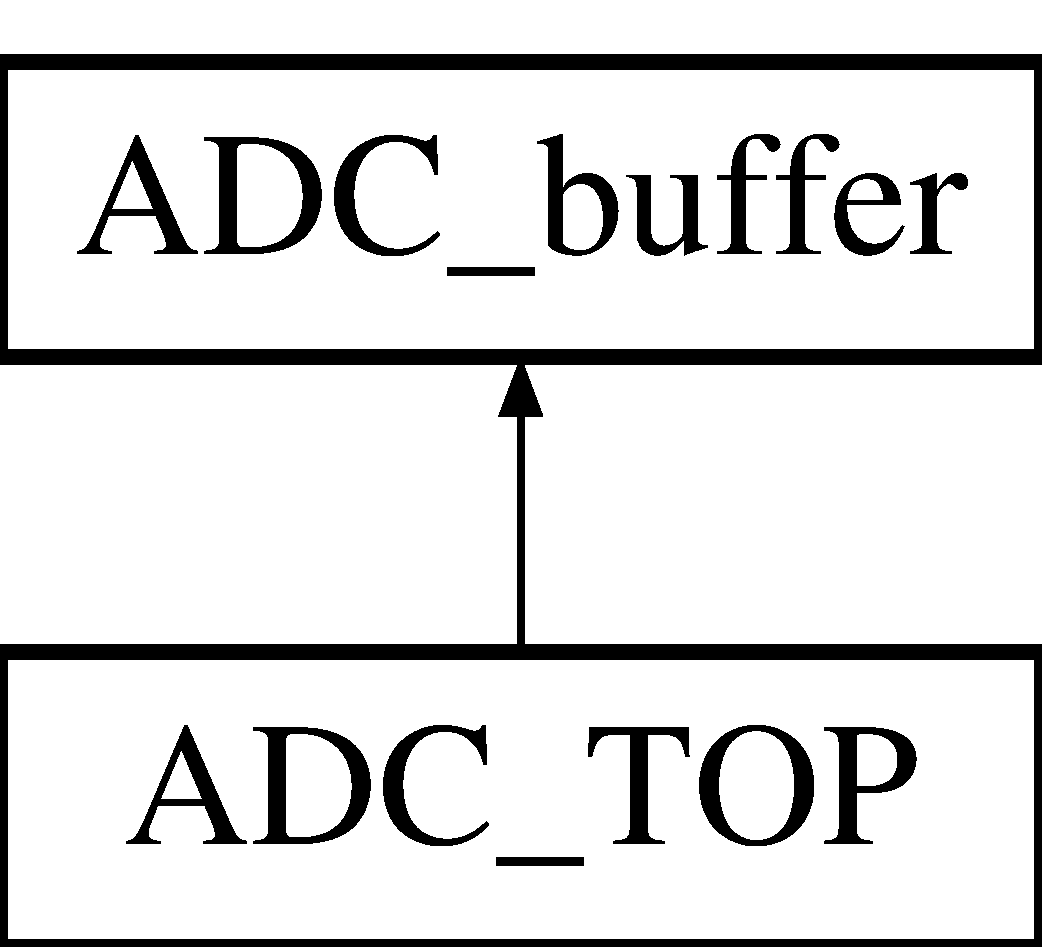
\includegraphics[height=2.000000cm]{classADC__buffer}
\end{center}
\end{figure}
\subsection*{Entities}
\begin{DoxyCompactItemize}
\item 
\hyperlink{classADC__buffer_1_1Behavioral}{Behavioral} architecture
\begin{DoxyCompactList}\small\item\em Achitechture of the A\-D\-C buffer. \end{DoxyCompactList}\end{DoxyCompactItemize}
\subsection*{Libraries}
 \begin{DoxyCompactItemize}
\item 
\hypertarget{classADC__buffer_ae4f03c286607f3181e16b9aa12d0c6d4}{\hyperlink{classADC__buffer_ae4f03c286607f3181e16b9aa12d0c6d4}{I\-E\-E\-E} }\label{classADC__buffer_ae4f03c286607f3181e16b9aa12d0c6d4}

\begin{DoxyCompactList}\small\item\em Use of standard library. \end{DoxyCompactList}\end{DoxyCompactItemize}
\subsection*{Use Clauses}
 \begin{DoxyCompactItemize}
\item 
\hypertarget{classADC__buffer_a68c233289eaf7d2601307bdd93b4c299}{\hyperlink{classADC__buffer_a68c233289eaf7d2601307bdd93b4c299}{I\-E\-E\-E.\-S\-T\-D\-\_\-\-L\-O\-G\-I\-C\-\_\-1164.\-all}   }\label{classADC__buffer_a68c233289eaf7d2601307bdd93b4c299}

\begin{DoxyCompactList}\small\item\em Use of standard logic arguments. \end{DoxyCompactList}\item 
\hypertarget{classADC__buffer_a7c135c43c66ccd7f22abe5f6211788a5}{\hyperlink{classADC__buffer_a7c135c43c66ccd7f22abe5f6211788a5}{I\-E\-E\-E.\-N\-U\-M\-E\-R\-I\-C\-\_\-\-S\-T\-D.\-all}   }\label{classADC__buffer_a7c135c43c66ccd7f22abe5f6211788a5}

\begin{DoxyCompactList}\small\item\em Use of standard numerical arguments. \end{DoxyCompactList}\end{DoxyCompactItemize}
\subsection*{Generics}
 \begin{DoxyCompactItemize}
\item 
\hypertarget{classADC__buffer_a2f94b7b31a8914ee23be5e000f89e921}{\hyperlink{classADC__buffer_a2f94b7b31a8914ee23be5e000f89e921}{bufferwidth} {\bfseries {\bfseries \textcolor{comment}{integer}\textcolor{vhdlchar}{ }\textcolor{vhdlchar}{\-:}\textcolor{vhdlchar}{=}\textcolor{vhdlchar}{ } \textcolor{vhdldigit}{7} \textcolor{vhdlchar}{ }}}}\label{classADC__buffer_a2f94b7b31a8914ee23be5e000f89e921}

\begin{DoxyCompactList}\small\item\em Generic indicating the width of the buffer address. \end{DoxyCompactList}\end{DoxyCompactItemize}
\subsection*{Ports}
 \begin{DoxyCompactItemize}
\item 
\hypertarget{classADC__buffer_a8120037e0ee47c35ba2d79242209c72e}{\hyperlink{classADC__buffer_a8120037e0ee47c35ba2d79242209c72e}{clk}  {\bfseries {\bfseries \textcolor{vhdlkeyword}{in}\textcolor{vhdlchar}{ }}} {\bfseries \textcolor{comment}{S\-T\-D\-\_\-\-L\-O\-G\-I\-C}\textcolor{vhdlchar}{ }} }\label{classADC__buffer_a8120037e0ee47c35ba2d79242209c72e}

\begin{DoxyCompactList}\small\item\em clock for buffer registers. \end{DoxyCompactList}\item 
\hypertarget{classADC__buffer_aa7b7040844189161771c36cf6bbf172c}{\hyperlink{classADC__buffer_aa7b7040844189161771c36cf6bbf172c}{rst}  {\bfseries {\bfseries \textcolor{vhdlkeyword}{in}\textcolor{vhdlchar}{ }}} {\bfseries \textcolor{comment}{S\-T\-D\-\_\-\-L\-O\-G\-I\-C}\textcolor{vhdlchar}{ }} }\label{classADC__buffer_aa7b7040844189161771c36cf6bbf172c}

\begin{DoxyCompactList}\small\item\em Global reset, active low. \end{DoxyCompactList}\item 
\hypertarget{classADC__buffer_a06ea925ba19422158afb079d09e4a231}{\hyperlink{classADC__buffer_a06ea925ba19422158afb079d09e4a231}{buff\-\_\-write}  {\bfseries {\bfseries \textcolor{vhdlkeyword}{in}\textcolor{vhdlchar}{ }}} {\bfseries \textcolor{comment}{S\-T\-D\-\_\-\-L\-O\-G\-I\-C}\textcolor{vhdlchar}{ }} }\label{classADC__buffer_a06ea925ba19422158afb079d09e4a231}

\begin{DoxyCompactList}\small\item\em Controls when values are to be stored, also changes the buffer memory pointer. \end{DoxyCompactList}\item 
\hypertarget{classADC__buffer_a0edd6254bf58107fb2411cc4cab05201}{\hyperlink{classADC__buffer_a0edd6254bf58107fb2411cc4cab05201}{Buffin}  {\bfseries {\bfseries \textcolor{vhdlkeyword}{in}\textcolor{vhdlchar}{ }}} {\bfseries \textcolor{comment}{S\-T\-D\-\_\-\-L\-O\-G\-I\-C\-\_\-\-V\-E\-C\-T\-O\-R}\textcolor{vhdlchar}{ }\textcolor{vhdlchar}{(}\textcolor{vhdlchar}{ }\textcolor{vhdlchar}{ } \textcolor{vhdldigit}{15} \textcolor{vhdlchar}{ }\textcolor{vhdlchar}{ }\textcolor{vhdlchar}{ }\textcolor{vhdlkeyword}{downto}\textcolor{vhdlchar}{ }\textcolor{vhdlchar}{ }\textcolor{vhdlchar}{ } \textcolor{vhdldigit}{0} \textcolor{vhdlchar}{ }\textcolor{vhdlchar}{)}\textcolor{vhdlchar}{ }} }\label{classADC__buffer_a0edd6254bf58107fb2411cc4cab05201}

\begin{DoxyCompactList}\small\item\em Input value to be stored. \end{DoxyCompactList}\item 
\hypertarget{classADC__buffer_ae32ca2a63fbe2fd9bbe609ba799ce989}{\hyperlink{classADC__buffer_ae32ca2a63fbe2fd9bbe609ba799ce989}{Buffout}  {\bfseries {\bfseries \textcolor{vhdlkeyword}{out}\textcolor{vhdlchar}{ }}} {\bfseries \textcolor{comment}{S\-T\-D\-\_\-\-L\-O\-G\-I\-C\-\_\-\-V\-E\-C\-T\-O\-R}\textcolor{vhdlchar}{ }\textcolor{vhdlchar}{(}\textcolor{vhdlchar}{ }\textcolor{vhdlchar}{ } \textcolor{vhdldigit}{15} \textcolor{vhdlchar}{ }\textcolor{vhdlchar}{ }\textcolor{vhdlchar}{ }\textcolor{vhdlkeyword}{downto}\textcolor{vhdlchar}{ }\textcolor{vhdlchar}{ }\textcolor{vhdlchar}{ } \textcolor{vhdldigit}{0} \textcolor{vhdlchar}{ }\textcolor{vhdlchar}{)}\textcolor{vhdlchar}{ }} }\label{classADC__buffer_ae32ca2a63fbe2fd9bbe609ba799ce989}

\begin{DoxyCompactList}\small\item\em Output value from the current address slot. \end{DoxyCompactList}\item 
\hypertarget{classADC__buffer_a4f849708d4274223b88930c2568f405c}{\hyperlink{classADC__buffer_a4f849708d4274223b88930c2568f405c}{Bufferfull}  {\bfseries {\bfseries \textcolor{vhdlkeyword}{out}\textcolor{vhdlchar}{ }}} {\bfseries \textcolor{comment}{S\-T\-D\-\_\-\-L\-O\-G\-I\-C}\textcolor{vhdlchar}{ }} }\label{classADC__buffer_a4f849708d4274223b88930c2568f405c}

\begin{DoxyCompactList}\small\item\em high for one clockcycle when the buffer is full, low otherwise. This is due to leon 3 only accepting interupts being high for one clockcycle. \end{DoxyCompactList}\item 
\hypertarget{classADC__buffer_ab93f1c6757ecccdcea2252108bb7caff}{\hyperlink{classADC__buffer_ab93f1c6757ecccdcea2252108bb7caff}{Addr}  {\bfseries {\bfseries \textcolor{vhdlkeyword}{in}\textcolor{vhdlchar}{ }}} {\bfseries \textcolor{comment}{S\-T\-D\-\_\-\-L\-O\-G\-I\-C\-\_\-\-V\-E\-C\-T\-O\-R}\textcolor{vhdlchar}{ }\textcolor{vhdlchar}{(}\textcolor{vhdlchar}{ }\textcolor{vhdlchar}{ }{\bfseries \hyperlink{classADC__buffer_a2f94b7b31a8914ee23be5e000f89e921}{bufferwidth}} \textcolor{vhdlchar}{ }\textcolor{vhdlchar}{-\/}\textcolor{vhdlchar}{ } \textcolor{vhdldigit}{1} \textcolor{vhdlchar}{ }\textcolor{vhdlchar}{ }\textcolor{vhdlchar}{ }\textcolor{vhdlkeyword}{downto}\textcolor{vhdlchar}{ }\textcolor{vhdlchar}{ }\textcolor{vhdlchar}{ } \textcolor{vhdldigit}{0} \textcolor{vhdlchar}{ }\textcolor{vhdlchar}{)}\textcolor{vhdlchar}{ }} }\label{classADC__buffer_ab93f1c6757ecccdcea2252108bb7caff}

\begin{DoxyCompactList}\small\item\em Address currently asked for. \end{DoxyCompactList}\end{DoxyCompactItemize}


\subsection{Detailed Description}
This component buffers samples when buff\-\_\-write goes from low to high, until the buffer is full. When this happens Buffer full is driven high for one clock cycle. The softcore will the read the values from the buffer by chaning the adress. The buffer will then instantly output the value on this address on the buffout port. 

The documentation for this class was generated from the following file\-:\begin{DoxyCompactItemize}
\item 
\hyperlink{ADC__buffer_8vhd}{A\-D\-C\-\_\-buffer.\-vhd}\end{DoxyCompactItemize}

\hypertarget{classADC__TOP}{\section{A\-D\-C\-\_\-\-T\-O\-P Entity Reference}
\label{classADC__TOP}\index{A\-D\-C\-\_\-\-T\-O\-P@{A\-D\-C\-\_\-\-T\-O\-P}}
}


Use of standard logic arguments.  


Inheritance diagram for A\-D\-C\-\_\-\-T\-O\-P\-:\begin{figure}[H]
\begin{center}
\leavevmode
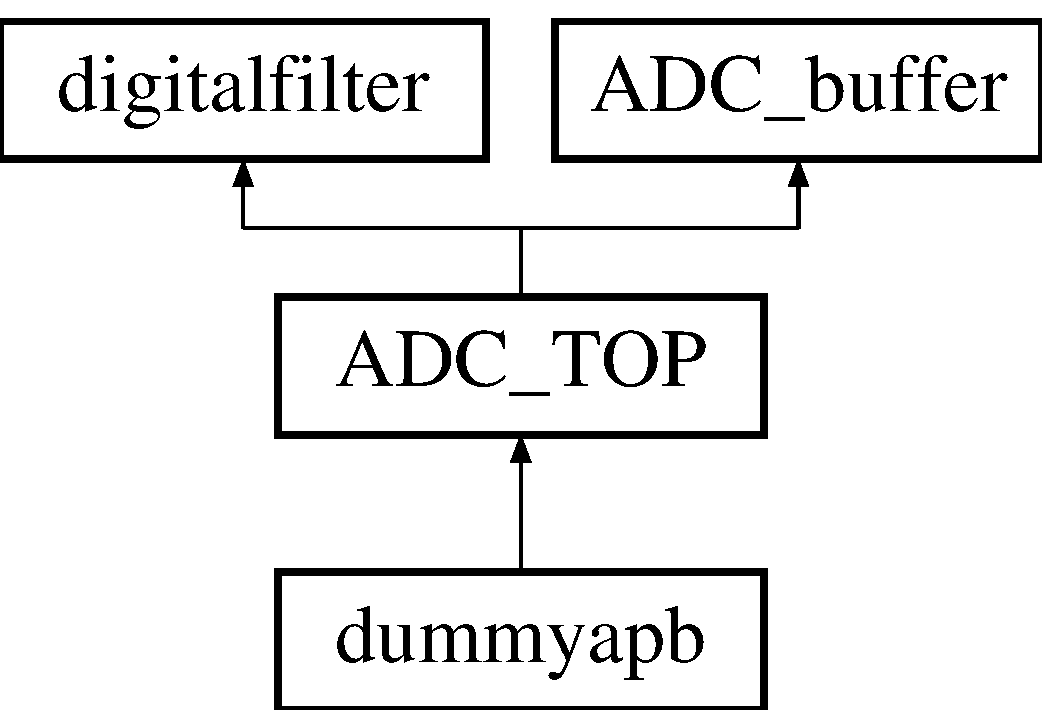
\includegraphics[height=2.000000cm]{classADC__TOP}
\end{center}
\end{figure}
\subsection*{Entities}
\begin{DoxyCompactItemize}
\item 
\hyperlink{classADC__TOP_1_1Behavioral}{Behavioral} architecture
\begin{DoxyCompactList}\small\item\em Architecture of the \hyperlink{classADC__TOP}{A\-D\-C\-\_\-\-T\-O\-P}. \end{DoxyCompactList}\end{DoxyCompactItemize}
\subsection*{Libraries}
 \begin{DoxyCompactItemize}
\item 
\hypertarget{classADC__TOP_ae4f03c286607f3181e16b9aa12d0c6d4}{\hyperlink{classADC__TOP_ae4f03c286607f3181e16b9aa12d0c6d4}{I\-E\-E\-E} }\label{classADC__TOP_ae4f03c286607f3181e16b9aa12d0c6d4}

\begin{DoxyCompactList}\small\item\em This line outputs the value of the buffer of the current adress to the out port. \end{DoxyCompactList}\end{DoxyCompactItemize}
\subsection*{Use Clauses}
 \begin{DoxyCompactItemize}
\item 
\hypertarget{classADC__TOP_a68c233289eaf7d2601307bdd93b4c299}{\hyperlink{classADC__TOP_a68c233289eaf7d2601307bdd93b4c299}{I\-E\-E\-E.\-S\-T\-D\-\_\-\-L\-O\-G\-I\-C\-\_\-1164.\-all}   }\label{classADC__TOP_a68c233289eaf7d2601307bdd93b4c299}

\begin{DoxyCompactList}\small\item\em Use of standard library. \end{DoxyCompactList}\end{DoxyCompactItemize}
\subsection*{Ports}
 \begin{DoxyCompactItemize}
\item 
\hypertarget{classADC__TOP_a9a17c21e2258ab6c61274f510b7ec756}{\hyperlink{classADC__TOP_a9a17c21e2258ab6c61274f510b7ec756}{C\-L\-K}  {\bfseries {\bfseries \textcolor{vhdlkeyword}{in}\textcolor{vhdlchar}{ }}} {\bfseries \textcolor{comment}{S\-T\-D\-\_\-\-L\-O\-G\-I\-C}\textcolor{vhdlchar}{ }} }\label{classADC__TOP_a9a17c21e2258ab6c61274f510b7ec756}

\begin{DoxyCompactList}\small\item\em This component is a wrapper for the A\-D\-C, a buffer and the components needed to complete the decimation. Its main functionality is to provide for internal connections between the compontnets. Global clock running at 50 M\-Hz. \end{DoxyCompactList}\item 
\hypertarget{classADC__TOP_ab1f7becce7cb29d94bb2f2ec187f72a4}{\hyperlink{classADC__TOP_ab1f7becce7cb29d94bb2f2ec187f72a4}{C\-L\-K100}  {\bfseries {\bfseries \textcolor{vhdlkeyword}{in}\textcolor{vhdlchar}{ }}} {\bfseries \textcolor{comment}{S\-T\-D\-\_\-\-L\-O\-G\-I\-C}\textcolor{vhdlchar}{ }} }\label{classADC__TOP_ab1f7becce7cb29d94bb2f2ec187f72a4}

\begin{DoxyCompactList}\small\item\em A clock on 100\-M\-Hz to let the filter have more taps. \end{DoxyCompactList}\item 
\hypertarget{classADC__TOP_a91cf794d165cc0a740042335a6062940}{\hyperlink{classADC__TOP_a91cf794d165cc0a740042335a6062940}{R\-S\-T}  {\bfseries {\bfseries \textcolor{vhdlkeyword}{in}\textcolor{vhdlchar}{ }}} {\bfseries \textcolor{comment}{S\-T\-D\-\_\-\-L\-O\-G\-I\-C}\textcolor{vhdlchar}{ }} }\label{classADC__TOP_a91cf794d165cc0a740042335a6062940}

\begin{DoxyCompactList}\small\item\em Global reset active low. \end{DoxyCompactList}\item 
\hypertarget{classADC__TOP_a4696bc4e06c727fae1b8ce3ba8cf08d4}{\hyperlink{classADC__TOP_a4696bc4e06c727fae1b8ce3ba8cf08d4}{sampleclk}  {\bfseries {\bfseries \textcolor{vhdlkeyword}{in}\textcolor{vhdlchar}{ }}} {\bfseries \textcolor{comment}{S\-T\-D\-\_\-\-L\-O\-G\-I\-C}\textcolor{vhdlchar}{ }} }\label{classADC__TOP_a4696bc4e06c727fae1b8ce3ba8cf08d4}

\begin{DoxyCompactList}\small\item\em Sample enable running at $\sim$44100 Hz. \end{DoxyCompactList}\item 
\hypertarget{classADC__TOP_af2205ffee98e5aeaa144186159740393}{\hyperlink{classADC__TOP_af2205ffee98e5aeaa144186159740393}{vauxp3}  {\bfseries {\bfseries \textcolor{vhdlkeyword}{in}\textcolor{vhdlchar}{ }}} {\bfseries \textcolor{comment}{S\-T\-D\-\_\-\-L\-O\-G\-I\-C}\textcolor{vhdlchar}{ }} }\label{classADC__TOP_af2205ffee98e5aeaa144186159740393}

\begin{DoxyCompactList}\small\item\em Positive analogue signal. \end{DoxyCompactList}\item 
\hypertarget{classADC__TOP_a3d034bd2912bb721a5bd221c185c5c99}{\hyperlink{classADC__TOP_a3d034bd2912bb721a5bd221c185c5c99}{vauxn3}  {\bfseries {\bfseries \textcolor{vhdlkeyword}{in}\textcolor{vhdlchar}{ }}} {\bfseries \textcolor{comment}{S\-T\-D\-\_\-\-L\-O\-G\-I\-C}\textcolor{vhdlchar}{ }} }\label{classADC__TOP_a3d034bd2912bb721a5bd221c185c5c99}

\begin{DoxyCompactList}\small\item\em Negative analogue signal. \end{DoxyCompactList}\item 
\hypertarget{classADC__TOP_a57ff14de06cd6f4e021faa435aae362b}{\hyperlink{classADC__TOP_a57ff14de06cd6f4e021faa435aae362b}{addr}  {\bfseries {\bfseries \textcolor{vhdlkeyword}{in}\textcolor{vhdlchar}{ }}} {\bfseries \textcolor{comment}{S\-T\-D\-\_\-\-L\-O\-G\-I\-C\-\_\-vector}\textcolor{vhdlchar}{ }\textcolor{vhdlchar}{(}\textcolor{vhdlchar}{ }\textcolor{vhdlchar}{ } \textcolor{vhdldigit}{6} \textcolor{vhdlchar}{ }\textcolor{vhdlchar}{ }\textcolor{vhdlchar}{ }\textcolor{vhdlkeyword}{downto}\textcolor{vhdlchar}{ }\textcolor{vhdlchar}{ }\textcolor{vhdlchar}{ } \textcolor{vhdldigit}{0} \textcolor{vhdlchar}{ }\textcolor{vhdlchar}{)}\textcolor{vhdlchar}{ }} }\label{classADC__TOP_a57ff14de06cd6f4e021faa435aae362b}

\begin{DoxyCompactList}\small\item\em Adress from the softcore. \end{DoxyCompactList}\item 
\hypertarget{classADC__TOP_a1db73b91cf59fc8a5c0e360bbc004989}{\hyperlink{classADC__TOP_a1db73b91cf59fc8a5c0e360bbc004989}{buff\-\_\-full}  {\bfseries {\bfseries \textcolor{vhdlkeyword}{out}\textcolor{vhdlchar}{ }}} {\bfseries \textcolor{comment}{S\-T\-D\-\_\-\-L\-O\-G\-I\-C}\textcolor{vhdlchar}{ }} }\label{classADC__TOP_a1db73b91cf59fc8a5c0e360bbc004989}

\begin{DoxyCompactList}\small\item\em Signal indicating the buffer is full. \end{DoxyCompactList}\item 
\hypertarget{classADC__TOP_a854e269333aa7d7b4c2241ff9e71aaf2}{\hyperlink{classADC__TOP_a854e269333aa7d7b4c2241ff9e71aaf2}{A\-D\-C\-\_\-buff\-\_\-write}  {\bfseries {\bfseries \textcolor{vhdlkeyword}{in}\textcolor{vhdlchar}{ }}} {\bfseries \textcolor{comment}{S\-T\-D\-\_\-\-L\-O\-G\-I\-C}\textcolor{vhdlchar}{ }} }\label{classADC__TOP_a854e269333aa7d7b4c2241ff9e71aaf2}

\begin{DoxyCompactList}\small\item\em Signal indicatig the buffer should be written. \end{DoxyCompactList}\item 
\hypertarget{classADC__TOP_a227e2ba1cceb52f292ef5768f933ba98}{\hyperlink{classADC__TOP_a227e2ba1cceb52f292ef5768f933ba98}{A\-D\-C\-\_\-buff\-\_\-out}  {\bfseries {\bfseries \textcolor{vhdlkeyword}{out}\textcolor{vhdlchar}{ }}} {\bfseries \textcolor{comment}{S\-T\-D\-\_\-\-L\-O\-G\-I\-C\-\_\-\-V\-E\-C\-T\-O\-R}\textcolor{vhdlchar}{ }\textcolor{vhdlchar}{(}\textcolor{vhdlchar}{ }\textcolor{vhdlchar}{ } \textcolor{vhdldigit}{15} \textcolor{vhdlchar}{ }\textcolor{vhdlchar}{ }\textcolor{vhdlchar}{ }\textcolor{vhdlkeyword}{downto}\textcolor{vhdlchar}{ }\textcolor{vhdlchar}{ }\textcolor{vhdlchar}{ } \textcolor{vhdldigit}{0} \textcolor{vhdlchar}{ }\textcolor{vhdlchar}{)}\textcolor{vhdlchar}{ }} }\label{classADC__TOP_a227e2ba1cceb52f292ef5768f933ba98}

\begin{DoxyCompactList}\small\item\em Sampled value after decimation. \end{DoxyCompactList}\end{DoxyCompactItemize}


\subsection{Detailed Description}
Use of standard logic arguments. 

The documentation for this class was generated from the following file\-:\begin{DoxyCompactItemize}
\item 
A\-D\-C\-\_\-\-T\-O\-P.\-vhd\end{DoxyCompactItemize}

\hypertarget{classdummyapb_1_1APB__interface}{\section{A\-P\-B\-\_\-interface Architecture Reference}
\label{classdummyapb_1_1APB__interface}\index{A\-P\-B\-\_\-interface@{A\-P\-B\-\_\-interface}}
}


Architecture of the Dummy\-\_\-apb.  


\subsection*{Processes}
 \begin{DoxyCompactItemize}
\item 
\hypertarget{classdummyapb_1_1APB__interface_a7b544993da64c8f112760250ae38b7cd}{\hyperlink{classdummyapb_1_1APB__interface_a7b544993da64c8f112760250ae38b7cd}{regs}{\bfseries  ( {\bfseries {\bfseries \hyperlink{classdummyapb_af1c59ef8e5ba3edeeb313b4be18d7d8a}{clk}} \textcolor{vhdlchar}{ }\textcolor{vhdlchar}{ }\textcolor{vhdlchar}{ }} , {\bfseries {\bfseries \hyperlink{classdummyapb_a8fb8388e1e2f3ac69332573f5909b4e8}{rstn}} \textcolor{vhdlchar}{ }} )}}\label{classdummyapb_1_1APB__interface_a7b544993da64c8f112760250ae38b7cd}

\end{DoxyCompactItemize}
\subsection*{Components}
 \begin{DoxyCompactItemize}
\item 
\hypertarget{classdummyapb_1_1APB__interface_a7a18f50a54f16177c6eca989b84ebc7b}{\hyperlink{classdummyapb_1_1APB__interface_a7a18f50a54f16177c6eca989b84ebc7b}{A\-D\-C\-\_\-\-T\-O\-P}  {\bfseries }  }\label{classdummyapb_1_1APB__interface_a7a18f50a54f16177c6eca989b84ebc7b}

\item 
\hypertarget{classdummyapb_1_1APB__interface_a68dc652e5df1fbc5e0657ac2658c7be2}{\hyperlink{classdummyapb_1_1APB__interface_a68dc652e5df1fbc5e0657ac2658c7be2}{Dac\-Top}  {\bfseries }  }\label{classdummyapb_1_1APB__interface_a68dc652e5df1fbc5e0657ac2658c7be2}

\end{DoxyCompactItemize}
\subsection*{Constants}
 \begin{DoxyCompactItemize}
\item 
\hypertarget{classdummyapb_1_1APB__interface_ac719d70a76e9eda27e2a22e4a55bb0c6}{\hyperlink{classdummyapb_1_1APB__interface_ac719d70a76e9eda27e2a22e4a55bb0c6}{pconfig} {\bfseries \textcolor{vhdlchar}{apb\-\_\-config\-\_\-type}\textcolor{vhdlchar}{ }\textcolor{vhdlchar}{ }\textcolor{vhdlchar}{\-:}\textcolor{vhdlchar}{=}\textcolor{vhdlchar}{ }\textcolor{vhdlchar}{ }\textcolor{vhdlchar}{(}\textcolor{vhdlchar}{ }\textcolor{vhdlchar}{ } \textcolor{vhdldigit}{0} \textcolor{vhdlchar}{ }\textcolor{vhdlchar}{ }\textcolor{vhdlchar}{=}\textcolor{vhdlchar}{ }\textcolor{vhdlchar}{$>$}\textcolor{vhdlchar}{ }\textcolor{vhdlchar}{ahb\-\_\-device\-\_\-reg}\textcolor{vhdlchar}{ }\textcolor{vhdlchar}{(}\textcolor{vhdlchar}{ }\textcolor{vhdlchar}{ }\textcolor{vhdlchar}{V\-E\-N\-D\-O\-R\-\_\-\-G\-R\-O\-U\-P}\textcolor{vhdlchar}{ }\textcolor{vhdlchar}{,}\textcolor{vhdlchar}{ }\textcolor{vhdlchar}{ }\textcolor{vhdlchar}{O\-W\-N\-\_\-\-A\-D\-C}\textcolor{vhdlchar}{ }\textcolor{vhdlchar}{,}\textcolor{vhdlchar}{ }\textcolor{vhdlchar}{ } \textcolor{vhdldigit}{0} \textcolor{vhdlchar}{ }\textcolor{vhdlchar}{,}\textcolor{vhdlchar}{ }\textcolor{vhdlchar}{ } \textcolor{vhdldigit}{0} \textcolor{vhdlchar}{ }\textcolor{vhdlchar}{,}\textcolor{vhdlchar}{ }\textcolor{vhdlchar}{ } \textcolor{vhdldigit}{0} \textcolor{vhdlchar}{ }\textcolor{vhdlchar}{)}\textcolor{vhdlchar}{ }\textcolor{vhdlchar}{,}\textcolor{vhdlchar}{ }\textcolor{vhdlchar}{ } \textcolor{vhdldigit}{1} \textcolor{vhdlchar}{ }\textcolor{vhdlchar}{ }\textcolor{vhdlchar}{=}\textcolor{vhdlchar}{ }\textcolor{vhdlchar}{$>$}\textcolor{vhdlchar}{ }\textcolor{vhdlchar}{apb\-\_\-iobar}\textcolor{vhdlchar}{ }\textcolor{vhdlchar}{(}\textcolor{vhdlchar}{ }\textcolor{vhdlchar}{ }{\bfseries \hyperlink{classdummyapb_a1c4c90775fe1a0af1ff79546ceb2f9c2}{paddr}} \textcolor{vhdlchar}{ }\textcolor{vhdlchar}{,}\textcolor{vhdlchar}{ }\textcolor{vhdlchar}{ }{\bfseries \hyperlink{classdummyapb_ae4b21043dd0ec623e5b8ed1cbe9db7b5}{pmask}} \textcolor{vhdlchar}{ }\textcolor{vhdlchar}{)}\textcolor{vhdlchar}{ }\textcolor{vhdlchar}{ }\textcolor{vhdlchar}{)}\textcolor{vhdlchar}{ }} }\label{classdummyapb_1_1APB__interface_ac719d70a76e9eda27e2a22e4a55bb0c6}

\end{DoxyCompactItemize}
\subsection*{Signals}
 \begin{DoxyCompactItemize}
\item 
\hypertarget{classdummyapb_1_1APB__interface_ae0194d89ba0e5c1d6f2cd0ca4de6944a}{\hyperlink{classdummyapb_1_1APB__interface_ae0194d89ba0e5c1d6f2cd0ca4de6944a}{s\-L\-E\-D} {\bfseries \textcolor{comment}{std\-\_\-logic\-\_\-vector}\textcolor{vhdlchar}{ }\textcolor{vhdlchar}{(}\textcolor{vhdlchar}{ }\textcolor{vhdlchar}{ } \textcolor{vhdldigit}{31} \textcolor{vhdlchar}{ }\textcolor{vhdlchar}{ }\textcolor{vhdlchar}{ }\textcolor{vhdlkeyword}{downto}\textcolor{vhdlchar}{ }\textcolor{vhdlchar}{ }\textcolor{vhdlchar}{ } \textcolor{vhdldigit}{0} \textcolor{vhdlchar}{ }\textcolor{vhdlchar}{)}\textcolor{vhdlchar}{ }} }\label{classdummyapb_1_1APB__interface_ae0194d89ba0e5c1d6f2cd0ca4de6944a}

\begin{DoxyCompactList}\small\item\em Buffered signals from the A\-P\-B bus. \end{DoxyCompactList}\item 
\hypertarget{classdummyapb_1_1APB__interface_ad5797d4ae2d654477e555700f8c3e43f}{\hyperlink{classdummyapb_1_1APB__interface_ad5797d4ae2d654477e555700f8c3e43f}{sampledvalue} {\bfseries \textcolor{comment}{S\-T\-D\-\_\-\-L\-O\-G\-I\-C\-\_\-\-V\-E\-C\-T\-O\-R}\textcolor{vhdlchar}{ }\textcolor{vhdlchar}{(}\textcolor{vhdlchar}{ }\textcolor{vhdlchar}{ } \textcolor{vhdldigit}{15} \textcolor{vhdlchar}{ }\textcolor{vhdlchar}{ }\textcolor{vhdlchar}{ }\textcolor{vhdlkeyword}{downto}\textcolor{vhdlchar}{ }\textcolor{vhdlchar}{ }\textcolor{vhdlchar}{ } \textcolor{vhdldigit}{0} \textcolor{vhdlchar}{ }\textcolor{vhdlchar}{)}\textcolor{vhdlchar}{ }} }\label{classdummyapb_1_1APB__interface_ad5797d4ae2d654477e555700f8c3e43f}

\begin{DoxyCompactList}\small\item\em Sampled value from the \hyperlink{classADC__buffer}{A\-D\-C\-\_\-buffer}. \end{DoxyCompactList}\item 
\hypertarget{classdummyapb_1_1APB__interface_a3201935a6a12fb549d5d5859e2883faf}{\hyperlink{classdummyapb_1_1APB__interface_a3201935a6a12fb549d5d5859e2883faf}{sampleclk} {\bfseries \textcolor{comment}{std\-\_\-logic}\textcolor{vhdlchar}{ }} }\label{classdummyapb_1_1APB__interface_a3201935a6a12fb549d5d5859e2883faf}

\begin{DoxyCompactList}\small\item\em Sample clock for the A\-D\-C. \end{DoxyCompactList}\item 
\hypertarget{classdummyapb_1_1APB__interface_a2d5fd474752c55aa67756b168d9f7fed}{\hyperlink{classdummyapb_1_1APB__interface_a2d5fd474752c55aa67756b168d9f7fed}{A\-D\-D\-R} {\bfseries \textcolor{comment}{S\-T\-D\-\_\-\-L\-O\-G\-I\-C\-\_\-\-V\-E\-C\-T\-O\-R}\textcolor{vhdlchar}{ }\textcolor{vhdlchar}{(}\textcolor{vhdlchar}{ }\textcolor{vhdlchar}{ } \textcolor{vhdldigit}{6} \textcolor{vhdlchar}{ }\textcolor{vhdlchar}{ }\textcolor{vhdlchar}{ }\textcolor{vhdlkeyword}{downto}\textcolor{vhdlchar}{ }\textcolor{vhdlchar}{ }\textcolor{vhdlchar}{ } \textcolor{vhdldigit}{0} \textcolor{vhdlchar}{ }\textcolor{vhdlchar}{)}\textcolor{vhdlchar}{ }} }\label{classdummyapb_1_1APB__interface_a2d5fd474752c55aa67756b168d9f7fed}

\begin{DoxyCompactList}\small\item\em Address for the \hyperlink{classADC__buffer}{A\-D\-C\-\_\-buffer} and D\-A\-C\-\_\-buffers. \end{DoxyCompactList}\item 
\hypertarget{classdummyapb_1_1APB__interface_aea49d8614e8eb0ad6fa3379810e11687}{\hyperlink{classdummyapb_1_1APB__interface_aea49d8614e8eb0ad6fa3379810e11687}{buffer\-\_\-interupt} {\bfseries \textcolor{comment}{S\-T\-D\-\_\-\-L\-O\-G\-I\-C}\textcolor{vhdlchar}{ }} }\label{classdummyapb_1_1APB__interface_aea49d8614e8eb0ad6fa3379810e11687}

\begin{DoxyCompactList}\small\item\em Interrupt from the \hyperlink{classADC__buffer}{A\-D\-C\-\_\-buffer}. \end{DoxyCompactList}\item 
\hypertarget{classdummyapb_1_1APB__interface_a7ebb7c0c3278d3ee00b9d65950f460a1}{\hyperlink{classdummyapb_1_1APB__interface_a7ebb7c0c3278d3ee00b9d65950f460a1}{sampleena44k\-Hz} {\bfseries \textcolor{comment}{S\-T\-D\-\_\-\-L\-O\-G\-I\-C}\textcolor{vhdlchar}{ }} }\label{classdummyapb_1_1APB__interface_a7ebb7c0c3278d3ee00b9d65950f460a1}

\begin{DoxyCompactList}\small\item\em Sample clock for the A\-D\-C buffer. \end{DoxyCompactList}\item 
\hypertarget{classdummyapb_1_1APB__interface_a5b75e0ed5e3882a01953fb69419c92ae}{\hyperlink{classdummyapb_1_1APB__interface_a5b75e0ed5e3882a01953fb69419c92ae}{dac\-\_\-buff\-\_\-write} {\bfseries \textcolor{comment}{S\-T\-D\-\_\-\-L\-O\-G\-I\-C}\textcolor{vhdlchar}{ }} }\label{classdummyapb_1_1APB__interface_a5b75e0ed5e3882a01953fb69419c92ae}

\begin{DoxyCompactList}\small\item\em This signal comes from the right address combination indicating the \hyperlink{classDAC__buffer}{D\-A\-C\-\_\-buffer} is to read. \end{DoxyCompactList}\item 
\hypertarget{classdummyapb_1_1APB__interface_a769f70cbb5f735c15f487c59ff05b292}{\hyperlink{classdummyapb_1_1APB__interface_a769f70cbb5f735c15f487c59ff05b292}{irq} {\bfseries \textcolor{comment}{S\-T\-D\-\_\-\-L\-O\-G\-I\-C}\textcolor{vhdlchar}{ }} }\label{classdummyapb_1_1APB__interface_a769f70cbb5f735c15f487c59ff05b292}

\begin{DoxyCompactList}\small\item\em Buffered interrupt to prevent the interrupt if being high for more than one clock cycle. \end{DoxyCompactList}\end{DoxyCompactItemize}
\subsection*{Instantiations}
 \begin{DoxyCompactItemize}
\item 
\hypertarget{classdummyapb_1_1APB__interface_af8047950a8cbc047aafda26366d23dcd}{\hyperlink{classdummyapb_1_1APB__interface_af8047950a8cbc047aafda26366d23dcd}{inst\-\_\-top}  {\bfseries dactop}   }\label{classdummyapb_1_1APB__interface_af8047950a8cbc047aafda26366d23dcd}

\begin{DoxyCompactList}\small\item\em This vector configs the address ranging and start address. \end{DoxyCompactList}\item 
\hypertarget{classdummyapb_1_1APB__interface_af3a42d0acd19aeab2e861d729423303a}{\hyperlink{classdummyapb_1_1APB__interface_af3a42d0acd19aeab2e861d729423303a}{inst\-\_\-adc\-\_\-top}  {\bfseries A\-D\-C\-\_\-\-T\-O\-P}   }\label{classdummyapb_1_1APB__interface_af3a42d0acd19aeab2e861d729423303a}

\item 
\hypertarget{classdummyapb_1_1APB__interface_acc6b2c6c9f85f90e08b01fb364af1a87}{\hyperlink{classdummyapb_1_1APB__interface_acc6b2c6c9f85f90e08b01fb364af1a87}{bootmsg}  {\bfseries report\-\_\-version}   }\label{classdummyapb_1_1APB__interface_acc6b2c6c9f85f90e08b01fb364af1a87}

\end{DoxyCompactItemize}


\subsection{Detailed Description}
Architecture of the Dummy\-\_\-apb. 

The Dummy A\-P\-B creates an interface between the A\-P\-B and the A\-D\-C/\-D\-A\-C. This is done in the simplest way possible. The address to the A\-D\-C and D\-A\-C buffer is part of the A\-P\-B address to this component. 

The documentation for this class was generated from the following files\-:\begin{DoxyCompactItemize}
\item 
\hyperlink{dummyapb_8vhd}{dummyapb.\-vhd}\end{DoxyCompactItemize}

\hypertarget{classBCD__block}{\section{B\-C\-D\-\_\-block Entity Reference}
\label{classBCD__block}\index{B\-C\-D\-\_\-block@{B\-C\-D\-\_\-block}}
}


This module is used in the conversion of binary to binary coded decimals.  


Inheritance diagram for B\-C\-D\-\_\-block\-:\begin{figure}[H]
\begin{center}
\leavevmode
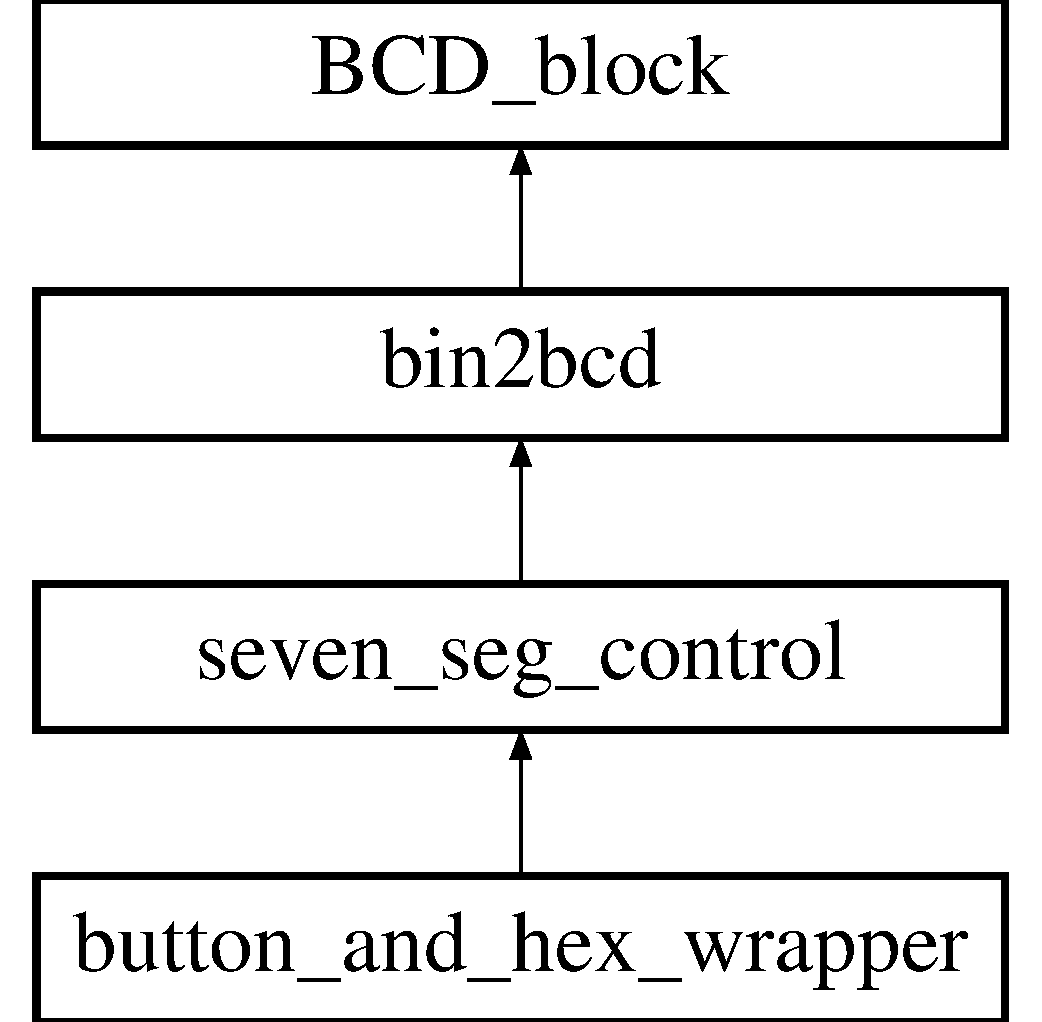
\includegraphics[height=4.000000cm]{classBCD__block}
\end{center}
\end{figure}
\subsection*{Entities}
\begin{DoxyCompactItemize}
\item 
\hyperlink{classBCD__block_1_1LUT}{L\-U\-T} architecture
\begin{DoxyCompactList}\small\item\em Architecture of the \hyperlink{classBCD__block}{B\-C\-D\-\_\-block}. \end{DoxyCompactList}\end{DoxyCompactItemize}
\subsection*{Libraries}
 \begin{DoxyCompactItemize}
\item 
\hypertarget{classBCD__block_ae4f03c286607f3181e16b9aa12d0c6d4}{\hyperlink{classBCD__block_ae4f03c286607f3181e16b9aa12d0c6d4}{I\-E\-E\-E} }\label{classBCD__block_ae4f03c286607f3181e16b9aa12d0c6d4}

\begin{DoxyCompactList}\small\item\em Use of standard library. \end{DoxyCompactList}\end{DoxyCompactItemize}
\subsection*{Use Clauses}
 \begin{DoxyCompactItemize}
\item 
\hypertarget{classBCD__block_a68c233289eaf7d2601307bdd93b4c299}{\hyperlink{classBCD__block_a68c233289eaf7d2601307bdd93b4c299}{I\-E\-E\-E.\-S\-T\-D\-\_\-\-L\-O\-G\-I\-C\-\_\-1164.\-all}   }\label{classBCD__block_a68c233289eaf7d2601307bdd93b4c299}

\begin{DoxyCompactList}\small\item\em Use of standard logic arguments. \end{DoxyCompactList}\end{DoxyCompactItemize}
\subsection*{Ports}
 \begin{DoxyCompactItemize}
\item 
\hypertarget{classBCD__block_a74bbc5867d62a92f3255225da1687bcb}{\hyperlink{classBCD__block_a74bbc5867d62a92f3255225da1687bcb}{in\-\_\-vector}  {\bfseries {\bfseries \textcolor{vhdlkeyword}{in}\textcolor{vhdlchar}{ }}} {\bfseries \textcolor{comment}{S\-T\-D\-\_\-\-L\-O\-G\-I\-C\-\_\-\-V\-E\-C\-T\-O\-R}\textcolor{vhdlchar}{ }\textcolor{vhdlchar}{(}\textcolor{vhdlchar}{ }\textcolor{vhdlchar}{ } \textcolor{vhdldigit}{3} \textcolor{vhdlchar}{ }\textcolor{vhdlchar}{ }\textcolor{vhdlchar}{ }\textcolor{vhdlkeyword}{downto}\textcolor{vhdlchar}{ }\textcolor{vhdlchar}{ }\textcolor{vhdlchar}{ } \textcolor{vhdldigit}{0} \textcolor{vhdlchar}{ }\textcolor{vhdlchar}{)}\textcolor{vhdlchar}{ }} }\label{classBCD__block_a74bbc5867d62a92f3255225da1687bcb}

\begin{DoxyCompactList}\small\item\em Input binary vector. \end{DoxyCompactList}\item 
\hypertarget{classBCD__block_a16d23e0812e4ff5fdb6428217589754d}{\hyperlink{classBCD__block_a16d23e0812e4ff5fdb6428217589754d}{out\-\_\-vector}  {\bfseries {\bfseries \textcolor{vhdlkeyword}{out}\textcolor{vhdlchar}{ }}} {\bfseries \textcolor{comment}{S\-T\-D\-\_\-\-L\-O\-G\-I\-C\-\_\-\-V\-E\-C\-T\-O\-R}\textcolor{vhdlchar}{ }\textcolor{vhdlchar}{(}\textcolor{vhdlchar}{ }\textcolor{vhdlchar}{ } \textcolor{vhdldigit}{3} \textcolor{vhdlchar}{ }\textcolor{vhdlchar}{ }\textcolor{vhdlchar}{ }\textcolor{vhdlkeyword}{downto}\textcolor{vhdlchar}{ }\textcolor{vhdlchar}{ }\textcolor{vhdlchar}{ } \textcolor{vhdldigit}{0} \textcolor{vhdlchar}{ }\textcolor{vhdlchar}{)}\textcolor{vhdlchar}{ }} }\label{classBCD__block_a16d23e0812e4ff5fdb6428217589754d}

\begin{DoxyCompactList}\small\item\em output B\-C\-D vector \end{DoxyCompactList}\end{DoxyCompactItemize}


\subsection{Detailed Description}
This module is used in the conversion of binary to binary coded decimals. 

The documentation for this class was generated from the following file\-:\begin{DoxyCompactItemize}
\item 
\hyperlink{BCD__block_8vhd}{B\-C\-D\-\_\-block.\-vhd}\end{DoxyCompactItemize}

\hypertarget{classbin2bcd}{\section{bin2bcd Entity Reference}
\label{classbin2bcd}\index{bin2bcd@{bin2bcd}}
}


This component calculates the binary coded decimal equivelent of a binary number. This module is not completely generec yet but it is verified to work at the size used in the implementation. For updates check \href{https://github.com/Jaxc/bin2bcd}{\tt https\-://github.\-com/\-Jaxc/bin2bcd}.  


Inheritance diagram for bin2bcd\-:\begin{figure}[H]
\begin{center}
\leavevmode
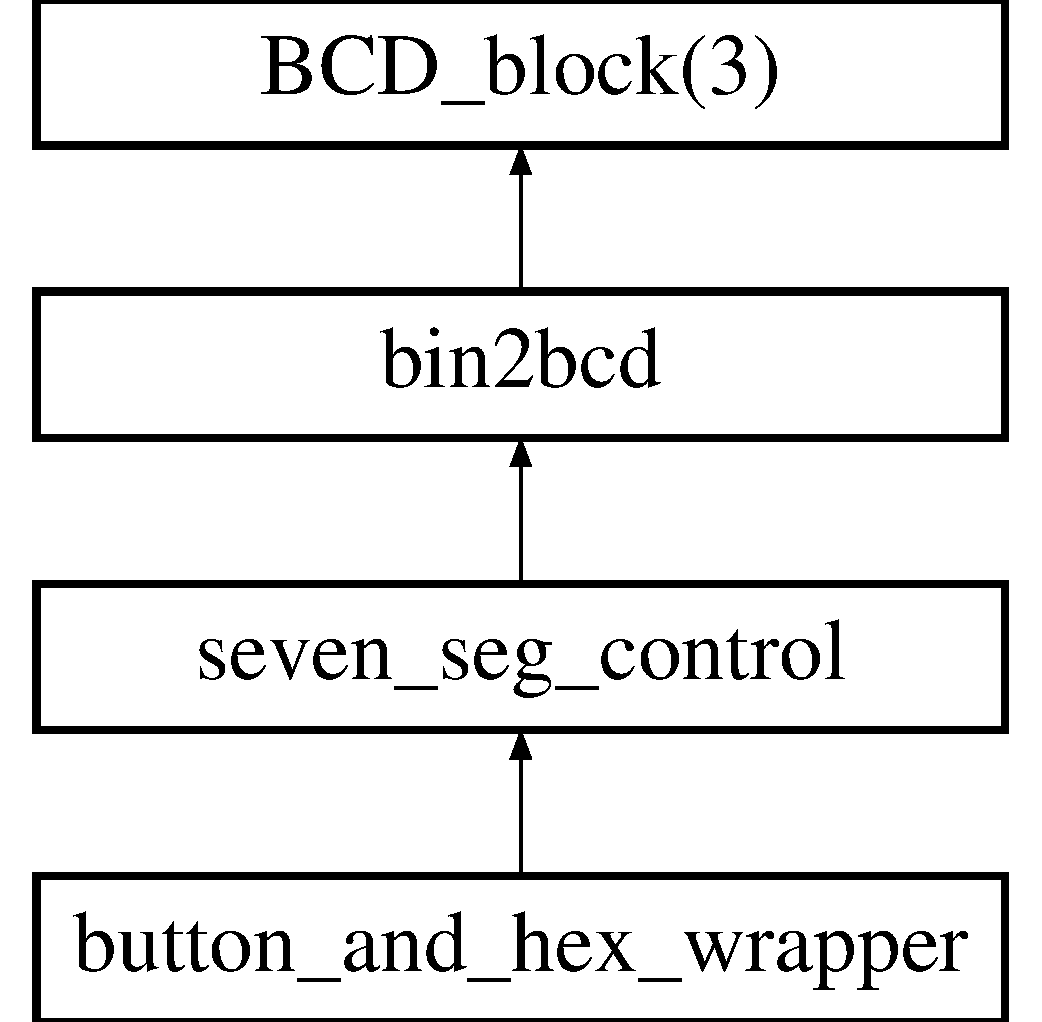
\includegraphics[height=4.000000cm]{classbin2bcd}
\end{center}
\end{figure}
\subsection*{Entities}
\begin{DoxyCompactItemize}
\item 
\hyperlink{classbin2bcd_1_1Behavioral}{Behavioral} architecture
\begin{DoxyCompactList}\small\item\em Achitechture of the \hyperlink{classbin2bcd}{bin2bcd}  component is a generic binary to binary coded decimal. It does this by using the \hyperlink{classBCD__block}{B\-C\-D\-\_\-block} according to the method used in \href{http://www.johnloomis.org/ece314/notes/devices/binary_to_BCD/bin_to_bcd.html}{\tt http\-://www.\-johnloomis.\-org/ece314/notes/devices/binary\-\_\-to\-\_\-\-B\-C\-D/bin\-\_\-to\-\_\-bcd.\-html}. \end{DoxyCompactList}\end{DoxyCompactItemize}
\subsection*{Libraries}
 \begin{DoxyCompactItemize}
\item 
\hypertarget{classbin2bcd_ae4f03c286607f3181e16b9aa12d0c6d4}{\hyperlink{classbin2bcd_ae4f03c286607f3181e16b9aa12d0c6d4}{I\-E\-E\-E} }\label{classbin2bcd_ae4f03c286607f3181e16b9aa12d0c6d4}

\begin{DoxyCompactList}\small\item\em Use of standard library. \end{DoxyCompactList}\end{DoxyCompactItemize}
\subsection*{Use Clauses}
 \begin{DoxyCompactItemize}
\item 
\hypertarget{classbin2bcd_a68c233289eaf7d2601307bdd93b4c299}{\hyperlink{classbin2bcd_a68c233289eaf7d2601307bdd93b4c299}{I\-E\-E\-E.\-S\-T\-D\-\_\-\-L\-O\-G\-I\-C\-\_\-1164.\-all}   }\label{classbin2bcd_a68c233289eaf7d2601307bdd93b4c299}

\begin{DoxyCompactList}\small\item\em Use of standard logic arguments. \end{DoxyCompactList}\item 
\hypertarget{classbin2bcd_a7c135c43c66ccd7f22abe5f6211788a5}{\hyperlink{classbin2bcd_a7c135c43c66ccd7f22abe5f6211788a5}{I\-E\-E\-E.\-N\-U\-M\-E\-R\-I\-C\-\_\-\-S\-T\-D.\-all}   }\label{classbin2bcd_a7c135c43c66ccd7f22abe5f6211788a5}

\begin{DoxyCompactList}\small\item\em Use of standard numerical arguments. \end{DoxyCompactList}\item 
\hypertarget{classbin2bcd_a8284ebf76bf629c58adbf8d637e8328b}{\hyperlink{classbin2bcd_a8284ebf76bf629c58adbf8d637e8328b}{I\-E\-E\-E.\-M\-A\-T\-H\-\_\-\-R\-E\-A\-L.\-all}   }\label{classbin2bcd_a8284ebf76bf629c58adbf8d637e8328b}

\begin{DoxyCompactList}\small\item\em Use of real math arguments to calculate generics. \end{DoxyCompactList}\end{DoxyCompactItemize}
\subsection*{Generics}
 \begin{DoxyCompactItemize}
\item 
\hypertarget{classbin2bcd_a03ce448558c2218cb8d7efccef340e15}{\hyperlink{classbin2bcd_a03ce448558c2218cb8d7efccef340e15}{bits} {\bfseries {\bfseries \textcolor{comment}{integer}\textcolor{vhdlchar}{ }\textcolor{vhdlchar}{\-:}\textcolor{vhdlchar}{=}\textcolor{vhdlchar}{ } \textcolor{vhdldigit}{8} \textcolor{vhdlchar}{ }}}}\label{classbin2bcd_a03ce448558c2218cb8d7efccef340e15}

\begin{DoxyCompactList}\small\item\em binary bit width \end{DoxyCompactList}\end{DoxyCompactItemize}
\subsection*{Ports}
 \begin{DoxyCompactItemize}
\item 
\hypertarget{classbin2bcd_ae61be7d0c2a4029f72fa99ab83ad96d2}{\hyperlink{classbin2bcd_ae61be7d0c2a4029f72fa99ab83ad96d2}{bin}  {\bfseries {\bfseries \textcolor{vhdlkeyword}{in}\textcolor{vhdlchar}{ }}} {\bfseries \textcolor{comment}{S\-T\-D\-\_\-\-L\-O\-G\-I\-C\-\_\-\-V\-E\-C\-T\-O\-R}\textcolor{vhdlchar}{ }\textcolor{vhdlchar}{(}\textcolor{vhdlchar}{ }\textcolor{vhdlchar}{ }{\bfseries \hyperlink{classbin2bcd_a03ce448558c2218cb8d7efccef340e15}{bits}} \textcolor{vhdlchar}{ }\textcolor{vhdlchar}{-\/}\textcolor{vhdlchar}{ } \textcolor{vhdldigit}{1} \textcolor{vhdlchar}{ }\textcolor{vhdlchar}{ }\textcolor{vhdlchar}{ }\textcolor{vhdlkeyword}{downto}\textcolor{vhdlchar}{ }\textcolor{vhdlchar}{ }\textcolor{vhdlchar}{ } \textcolor{vhdldigit}{0} \textcolor{vhdlchar}{ }\textcolor{vhdlchar}{)}\textcolor{vhdlchar}{ }} }\label{classbin2bcd_ae61be7d0c2a4029f72fa99ab83ad96d2}

\begin{DoxyCompactList}\small\item\em Binary input. \end{DoxyCompactList}\item 
\hypertarget{classbin2bcd_ac691a88cf4b7f8ed22a51c1b682e84aa}{\hyperlink{classbin2bcd_ac691a88cf4b7f8ed22a51c1b682e84aa}{B\-C\-D}  {\bfseries {\bfseries \textcolor{vhdlkeyword}{out}\textcolor{vhdlchar}{ }}} {\bfseries \textcolor{comment}{S\-T\-D\-\_\-\-L\-O\-G\-I\-C\-\_\-\-V\-E\-C\-T\-O\-R}\textcolor{vhdlchar}{ }\textcolor{vhdlchar}{(}\textcolor{vhdlchar}{ }\textcolor{vhdlchar}{ }{\bfseries \hyperlink{classbin2bcd_a03ce448558c2218cb8d7efccef340e15}{bits}} \textcolor{vhdlchar}{ }\textcolor{vhdlchar}{$\ast$}\textcolor{vhdlchar}{ } \textcolor{vhdldigit}{2} \textcolor{vhdlchar}{ }\textcolor{vhdlchar}{-\/}\textcolor{vhdlchar}{ } \textcolor{vhdldigit}{1} \textcolor{vhdlchar}{ }\textcolor{vhdlchar}{ }\textcolor{vhdlchar}{ }\textcolor{vhdlkeyword}{downto}\textcolor{vhdlchar}{ }\textcolor{vhdlchar}{ }\textcolor{vhdlchar}{ } \textcolor{vhdldigit}{0} \textcolor{vhdlchar}{ }\textcolor{vhdlchar}{)}\textcolor{vhdlchar}{ }} }\label{classbin2bcd_ac691a88cf4b7f8ed22a51c1b682e84aa}

\begin{DoxyCompactList}\small\item\em B\-C\-D output. \end{DoxyCompactList}\end{DoxyCompactItemize}


\subsection{Detailed Description}
This component calculates the binary coded decimal equivelent of a binary number. This module is not completely generec yet but it is verified to work at the size used in the implementation. For updates check \href{https://github.com/Jaxc/bin2bcd}{\tt https\-://github.\-com/\-Jaxc/bin2bcd}. 

The documentation for this class was generated from the following file\-:\begin{DoxyCompactItemize}
\item 
\hyperlink{bin2bcd_8vhd}{bin2bcd.\-vhd}\end{DoxyCompactItemize}

\hypertarget{classbounce__filter}{\section{bounce\-\_\-filter Entity Reference}
\label{classbounce__filter}\index{bounce\-\_\-filter@{bounce\-\_\-filter}}
}


This component stabilized signals by waiting until a signal have been high or low for a set about of time.  


Inheritance diagram for bounce\-\_\-filter\-:\begin{figure}[H]
\begin{center}
\leavevmode
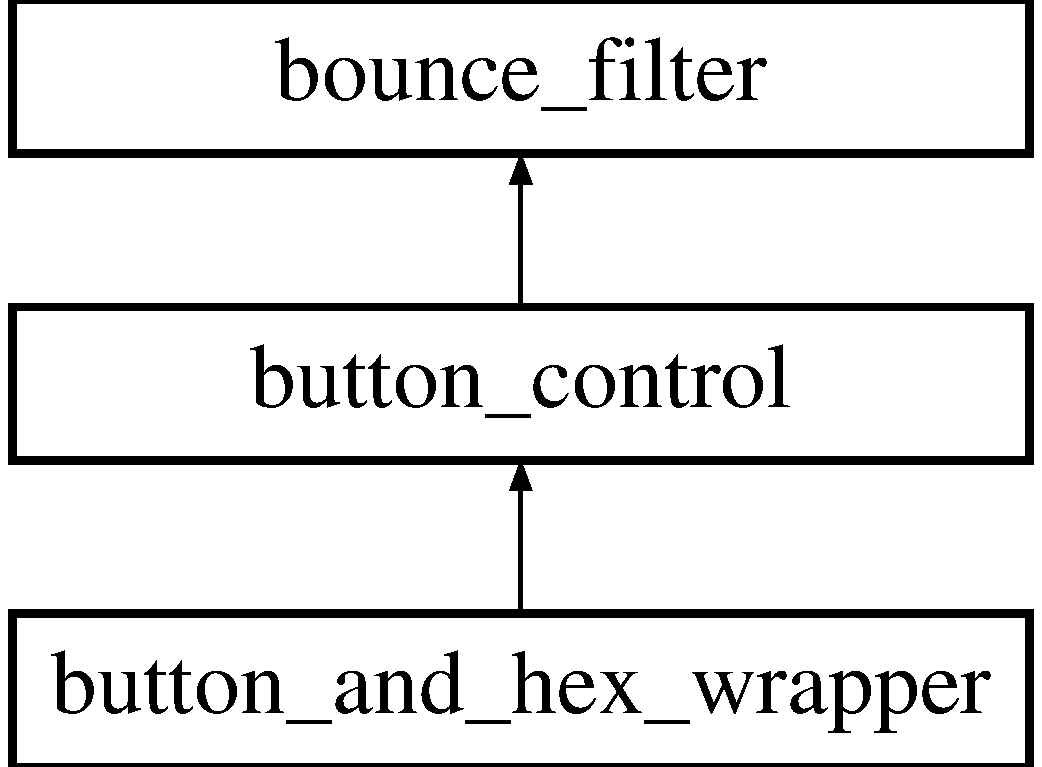
\includegraphics[height=3.000000cm]{classbounce__filter}
\end{center}
\end{figure}
\subsection*{Entities}
\begin{DoxyCompactItemize}
\item 
\hyperlink{classbounce__filter_1_1Behavioral}{Behavioral} architecture
\begin{DoxyCompactList}\small\item\em Architecture of the \hyperlink{classbounce__filter}{bounce\-\_\-filter}. \end{DoxyCompactList}\end{DoxyCompactItemize}
\subsection*{Libraries}
 \begin{DoxyCompactItemize}
\item 
\hypertarget{classbounce__filter_ae4f03c286607f3181e16b9aa12d0c6d4}{\hyperlink{classbounce__filter_ae4f03c286607f3181e16b9aa12d0c6d4}{I\-E\-E\-E} }\label{classbounce__filter_ae4f03c286607f3181e16b9aa12d0c6d4}

\begin{DoxyCompactList}\small\item\em Use of standard library. \end{DoxyCompactList}\end{DoxyCompactItemize}
\subsection*{Use Clauses}
 \begin{DoxyCompactItemize}
\item 
\hypertarget{classbounce__filter_a68c233289eaf7d2601307bdd93b4c299}{\hyperlink{classbounce__filter_a68c233289eaf7d2601307bdd93b4c299}{I\-E\-E\-E.\-S\-T\-D\-\_\-\-L\-O\-G\-I\-C\-\_\-1164.\-all}   }\label{classbounce__filter_a68c233289eaf7d2601307bdd93b4c299}

\begin{DoxyCompactList}\small\item\em Use of standard logic arguments. \end{DoxyCompactList}\item 
\hypertarget{classbounce__filter_a7c135c43c66ccd7f22abe5f6211788a5}{\hyperlink{classbounce__filter_a7c135c43c66ccd7f22abe5f6211788a5}{I\-E\-E\-E.\-N\-U\-M\-E\-R\-I\-C\-\_\-\-S\-T\-D.\-all}   }\label{classbounce__filter_a7c135c43c66ccd7f22abe5f6211788a5}

\begin{DoxyCompactList}\small\item\em Use of standard numerical arguments. \end{DoxyCompactList}\end{DoxyCompactItemize}
\subsection*{Generics}
 \begin{DoxyCompactItemize}
\item 
\hypertarget{classbounce__filter_a5df2a2aceb759129bf8abccdc30aec13}{\hyperlink{classbounce__filter_a5df2a2aceb759129bf8abccdc30aec13}{counterbits} {\bfseries {\bfseries \textcolor{comment}{integer}\textcolor{vhdlchar}{ }\textcolor{vhdlchar}{\-:}\textcolor{vhdlchar}{=}\textcolor{vhdlchar}{ } \textcolor{vhdldigit}{8} \textcolor{vhdlchar}{ }}}}\label{classbounce__filter_a5df2a2aceb759129bf8abccdc30aec13}

\begin{DoxyCompactList}\small\item\em Counter bits controls how many bits the counter will count before it changes value. \end{DoxyCompactList}\end{DoxyCompactItemize}
\subsection*{Ports}
 \begin{DoxyCompactItemize}
\item 
\hypertarget{classbounce__filter_a4e5c033a02939de1b3ca8aac83c35a39}{\hyperlink{classbounce__filter_a4e5c033a02939de1b3ca8aac83c35a39}{Button\-\_\-in}  {\bfseries {\bfseries \textcolor{vhdlkeyword}{in}\textcolor{vhdlchar}{ }}} {\bfseries \textcolor{comment}{S\-T\-D\-\_\-\-L\-O\-G\-I\-C}\textcolor{vhdlchar}{ }} }\label{classbounce__filter_a4e5c033a02939de1b3ca8aac83c35a39}

\begin{DoxyCompactList}\small\item\em Button\-\_\-in is the input to the fitler. \end{DoxyCompactList}\item 
\hypertarget{classbounce__filter_a8120037e0ee47c35ba2d79242209c72e}{\hyperlink{classbounce__filter_a8120037e0ee47c35ba2d79242209c72e}{clk}  {\bfseries {\bfseries \textcolor{vhdlkeyword}{in}\textcolor{vhdlchar}{ }}} {\bfseries \textcolor{comment}{S\-T\-D\-\_\-\-L\-O\-G\-I\-C}\textcolor{vhdlchar}{ }} }\label{classbounce__filter_a8120037e0ee47c35ba2d79242209c72e}

\begin{DoxyCompactList}\small\item\em Clock for counter and registers. \end{DoxyCompactList}\item 
\hypertarget{classbounce__filter_aba021aec4b477b89079bb58ccadcc67e}{\hyperlink{classbounce__filter_aba021aec4b477b89079bb58ccadcc67e}{rstn}  {\bfseries {\bfseries \textcolor{vhdlkeyword}{in}\textcolor{vhdlchar}{ }}} {\bfseries \textcolor{comment}{S\-T\-D\-\_\-\-L\-O\-G\-I\-C}\textcolor{vhdlchar}{ }} }\label{classbounce__filter_aba021aec4b477b89079bb58ccadcc67e}

\begin{DoxyCompactList}\small\item\em Global reset, active low. \end{DoxyCompactList}\item 
\hypertarget{classbounce__filter_a4411f41202f6d4784f12799680212e6d}{\hyperlink{classbounce__filter_a4411f41202f6d4784f12799680212e6d}{Button\-\_\-out}  {\bfseries {\bfseries \textcolor{vhdlkeyword}{out}\textcolor{vhdlchar}{ }}} {\bfseries \textcolor{comment}{S\-T\-D\-\_\-\-L\-O\-G\-I\-C}\textcolor{vhdlchar}{ }} }\label{classbounce__filter_a4411f41202f6d4784f12799680212e6d}

\begin{DoxyCompactList}\small\item\em Stabilized signal out. \end{DoxyCompactList}\end{DoxyCompactItemize}


\subsection{Detailed Description}
This component stabilized signals by waiting until a signal have been high or low for a set about of time. 

The documentation for this class was generated from the following file\-:\begin{DoxyCompactItemize}
\item 
\hyperlink{bounce__filter_8vhd}{bounce\-\_\-filter.\-vhd}\end{DoxyCompactItemize}

\hypertarget{classADC__buffer_1_1Buffer__ADC}{\section{Buffer\-\_\-\-A\-D\-C Architecture Reference}
\label{classADC__buffer_1_1Buffer__ADC}\index{Buffer\-\_\-\-A\-D\-C@{Buffer\-\_\-\-A\-D\-C}}
}


Architecture of the A\-D\-C buffer.  


\subsection*{Processes}
 \begin{DoxyCompactItemize}
\item 
\hypertarget{classADC__buffer_1_1Buffer__ADC_a7f0d4cc2572dde6003f96ff6890a2314}{\hyperlink{classADC__buffer_1_1Buffer__ADC_a7f0d4cc2572dde6003f96ff6890a2314}{P\-R\-O\-C\-E\-S\-S\-\_\-0}{\bfseries  ( {\bfseries {\bfseries \hyperlink{classADC__buffer_a8120037e0ee47c35ba2d79242209c72e}{clk}} \textcolor{vhdlchar}{ }\textcolor{vhdlchar}{ }\textcolor{vhdlchar}{ }} , {\bfseries {\bfseries \hyperlink{classADC__buffer_aa7b7040844189161771c36cf6bbf172c}{rst}} \textcolor{vhdlchar}{ }} )}}\label{classADC__buffer_1_1Buffer__ADC_a7f0d4cc2572dde6003f96ff6890a2314}

\begin{DoxyCompactList}\small\item\em The main process of the module. In this process handles the writing to the buffer. This process is Dependant on the clock and the reset. \end{DoxyCompactList}\end{DoxyCompactItemize}
\subsection*{Types}
 \begin{DoxyCompactItemize}
\item 
\hypertarget{classADC__buffer_1_1Buffer__ADC_a658e2166090ca64ce974029de2840027}{{\bfseries \hyperlink{classADC__buffer_1_1Buffer__ADC_a658e2166090ca64ce974029de2840027}{Memory\-\_\-array\-\_\-type}{\bfseries \textcolor{vhdlkeyword}{is}\textcolor{vhdlchar}{ }\textcolor{vhdlchar}{ }\textcolor{vhdlkeyword}{array}\textcolor{vhdlchar}{ }\textcolor{vhdlchar}{(}\textcolor{vhdlchar}{ } \textcolor{vhdldigit}{0} \textcolor{vhdlchar}{ }\textcolor{vhdlchar}{ }\textcolor{vhdlchar}{ }\textcolor{vhdlkeyword}{to}\textcolor{vhdlchar}{ }\textcolor{vhdlchar}{ }\textcolor{vhdlchar}{ } \textcolor{vhdldigit}{2} \textcolor{vhdlchar}{ }\textcolor{vhdlchar}{$\ast$}\textcolor{vhdlchar}{$\ast$}\textcolor{vhdlchar}{ }{\bfseries \hyperlink{classADC__buffer_a2f94b7b31a8914ee23be5e000f89e921}{bufferwidth}} \textcolor{vhdlchar}{ }\textcolor{vhdlchar}{-\/}\textcolor{vhdlchar}{ } \textcolor{vhdldigit}{1} \textcolor{vhdlchar}{ }\textcolor{vhdlchar}{)}\textcolor{vhdlchar}{ }\textcolor{vhdlchar}{ }\textcolor{vhdlkeyword}{of}\textcolor{vhdlchar}{ }\textcolor{comment}{S\-T\-D\-\_\-\-L\-O\-G\-I\-C\-\_\-\-V\-E\-C\-T\-O\-R}\textcolor{vhdlchar}{ }\textcolor{vhdlchar}{(}\textcolor{vhdlchar}{ }\textcolor{vhdlchar}{ } \textcolor{vhdldigit}{15} \textcolor{vhdlchar}{ }\textcolor{vhdlchar}{ }\textcolor{vhdlchar}{ }\textcolor{vhdlkeyword}{downto}\textcolor{vhdlchar}{ }\textcolor{vhdlchar}{ }\textcolor{vhdlchar}{ } \textcolor{vhdldigit}{0} \textcolor{vhdlchar}{ }}} }\label{classADC__buffer_1_1Buffer__ADC_a658e2166090ca64ce974029de2840027}

\begin{DoxyCompactList}\small\item\em The memory storage type. The type creates an array of a size of 2$^\wedge$bufferwidth$\ast$16. \end{DoxyCompactList}\end{DoxyCompactItemize}
\subsection*{Signals}
 \begin{DoxyCompactItemize}
\item 
\hypertarget{classADC__buffer_1_1Buffer__ADC_aa3242fe5cbe81a6710bd0ed34005d4ef}{\hyperlink{classADC__buffer_1_1Buffer__ADC_aa3242fe5cbe81a6710bd0ed34005d4ef}{Memory\-\_\-array} {\bfseries {\bfseries \hyperlink{classADC__buffer_1_1Buffer__ADC_a658e2166090ca64ce974029de2840027}{Memory\-\_\-array\-\_\-type}} \textcolor{vhdlchar}{ }} }\label{classADC__buffer_1_1Buffer__ADC_aa3242fe5cbe81a6710bd0ed34005d4ef}

\begin{DoxyCompactList}\small\item\em The actual memory storage element. This signal holds all of the stored elements. \end{DoxyCompactList}\item 
\hypertarget{classADC__buffer_1_1Buffer__ADC_ab722211b6f3f8617f6cf3e17336a0a12}{\hyperlink{classADC__buffer_1_1Buffer__ADC_ab722211b6f3f8617f6cf3e17336a0a12}{lastwrite} {\bfseries \textcolor{comment}{S\-T\-D\-\_\-\-L\-O\-G\-I\-C}\textcolor{vhdlchar}{ }} }\label{classADC__buffer_1_1Buffer__ADC_ab722211b6f3f8617f6cf3e17336a0a12}

\begin{DoxyCompactList}\small\item\em Lastwrite holds the last value of buff\-\_\-write to be able to detect a rising edge without using the signal as a clock. \end{DoxyCompactList}\item 
\hypertarget{classADC__buffer_1_1Buffer__ADC_a8333467b8d5554bb68347610f6060c42}{\hyperlink{classADC__buffer_1_1Buffer__ADC_a8333467b8d5554bb68347610f6060c42}{Write\-\_\-index} {\bfseries \textcolor{comment}{integer}\textcolor{vhdlchar}{ }\textcolor{vhdlkeyword}{range}\textcolor{vhdlchar}{ } \textcolor{vhdldigit}{0} \textcolor{vhdlchar}{ }\textcolor{vhdlchar}{ }\textcolor{vhdlchar}{ }\textcolor{vhdlkeyword}{to}\textcolor{vhdlchar}{ }\textcolor{vhdlchar}{ }\textcolor{vhdlchar}{ } \textcolor{vhdldigit}{2} \textcolor{vhdlchar}{ }\textcolor{vhdlchar}{$\ast$}\textcolor{vhdlchar}{$\ast$}\textcolor{vhdlchar}{ }{\bfseries \hyperlink{classADC__buffer_a2f94b7b31a8914ee23be5e000f89e921}{bufferwidth}} \textcolor{vhdlchar}{ }\textcolor{vhdlchar}{-\/}\textcolor{vhdlchar}{ } \textcolor{vhdldigit}{1} \textcolor{vhdlchar}{ }} }\label{classADC__buffer_1_1Buffer__ADC_a8333467b8d5554bb68347610f6060c42}

\begin{DoxyCompactList}\small\item\em Write\-\_\-index is a signal to indicate where the next value in the buffer is to be written. When this happens the write\-\_\-index is incremented by one. This makes the buffer write in a circular fashion. \end{DoxyCompactList}\end{DoxyCompactItemize}


\subsection{Detailed Description}
Architecture of the A\-D\-C buffer. 

The architecture containing the main body of the component. 

The documentation for this class was generated from the following file\-:\begin{DoxyCompactItemize}
\item 
\hyperlink{ADC__buffer_8vhd}{A\-D\-C\-\_\-buffer.\-vhd}\end{DoxyCompactItemize}

\hypertarget{classDAC__buffer_1_1Buffer__dac}{\section{Buffer\-\_\-dac Architecture Reference}
\label{classDAC__buffer_1_1Buffer__dac}\index{Buffer\-\_\-dac@{Buffer\-\_\-dac}}
}


Architecture of the D\-A\-C buffer.  


\subsection*{Processes}
 \begin{DoxyCompactItemize}
\item 
\hypertarget{classDAC__buffer_1_1Buffer__dac_a59eb74dc65f67582e3c037f7786d7adc}{\hyperlink{classDAC__buffer_1_1Buffer__dac_a59eb74dc65f67582e3c037f7786d7adc}{P\-R\-O\-C\-E\-S\-S\-\_\-6}{\bfseries  ( {\bfseries {\bfseries \hyperlink{classDAC__buffer_a8120037e0ee47c35ba2d79242209c72e}{clk}} \textcolor{vhdlchar}{ }\textcolor{vhdlchar}{ }\textcolor{vhdlchar}{ }} , {\bfseries {\bfseries \hyperlink{classDAC__buffer_aa7b7040844189161771c36cf6bbf172c}{rst}} \textcolor{vhdlchar}{ }} )}}\label{classDAC__buffer_1_1Buffer__dac_a59eb74dc65f67582e3c037f7786d7adc}

\end{DoxyCompactItemize}
\subsection*{Types}
 \begin{DoxyCompactItemize}
\item 
\hypertarget{classDAC__buffer_1_1Buffer__dac_a658e2166090ca64ce974029de2840027}{{\bfseries \hyperlink{classDAC__buffer_1_1Buffer__dac_a658e2166090ca64ce974029de2840027}{Memory\-\_\-array\-\_\-type}{\bfseries \textcolor{vhdlkeyword}{is}\textcolor{vhdlchar}{ }\textcolor{vhdlchar}{ }\textcolor{vhdlkeyword}{array}\textcolor{vhdlchar}{ }\textcolor{vhdlchar}{(}\textcolor{vhdlchar}{ } \textcolor{vhdldigit}{0} \textcolor{vhdlchar}{ }\textcolor{vhdlchar}{ }\textcolor{vhdlchar}{ }\textcolor{vhdlkeyword}{to}\textcolor{vhdlchar}{ }\textcolor{vhdlchar}{ }\textcolor{vhdlchar}{ } \textcolor{vhdldigit}{2} \textcolor{vhdlchar}{ }\textcolor{vhdlchar}{$\ast$}\textcolor{vhdlchar}{$\ast$}\textcolor{vhdlchar}{ }{\bfseries \hyperlink{classDAC__buffer_a2f94b7b31a8914ee23be5e000f89e921}{bufferwidth}} \textcolor{vhdlchar}{ }\textcolor{vhdlchar}{-\/}\textcolor{vhdlchar}{ } \textcolor{vhdldigit}{1} \textcolor{vhdlchar}{ }\textcolor{vhdlchar}{)}\textcolor{vhdlchar}{ }\textcolor{vhdlchar}{ }\textcolor{vhdlkeyword}{of}\textcolor{vhdlchar}{ }\textcolor{comment}{S\-T\-D\-\_\-\-L\-O\-G\-I\-C\-\_\-\-V\-E\-C\-T\-O\-R}\textcolor{vhdlchar}{ }\textcolor{vhdlchar}{(}\textcolor{vhdlchar}{ }\textcolor{vhdlchar}{ } \textcolor{vhdldigit}{15} \textcolor{vhdlchar}{ }\textcolor{vhdlchar}{ }\textcolor{vhdlchar}{ }\textcolor{vhdlkeyword}{downto}\textcolor{vhdlchar}{ }\textcolor{vhdlchar}{ }\textcolor{vhdlchar}{ } \textcolor{vhdldigit}{0} \textcolor{vhdlchar}{ }}} }\label{classDAC__buffer_1_1Buffer__dac_a658e2166090ca64ce974029de2840027}

\begin{DoxyCompactList}\small\item\em the type for the memory array, the length changes size due to a generic \end{DoxyCompactList}\end{DoxyCompactItemize}
\subsection*{Signals}
 \begin{DoxyCompactItemize}
\item 
\hypertarget{classDAC__buffer_1_1Buffer__dac_aa3242fe5cbe81a6710bd0ed34005d4ef}{\hyperlink{classDAC__buffer_1_1Buffer__dac_aa3242fe5cbe81a6710bd0ed34005d4ef}{Memory\-\_\-array} {\bfseries {\bfseries \hyperlink{classDAC__buffer_1_1Buffer__dac_a658e2166090ca64ce974029de2840027}{Memory\-\_\-array\-\_\-type}} \textcolor{vhdlchar}{ }} }\label{classDAC__buffer_1_1Buffer__dac_aa3242fe5cbe81a6710bd0ed34005d4ef}

\begin{DoxyCompactList}\small\item\em This signal is containing the buffered values. \end{DoxyCompactList}\item 
\hypertarget{classDAC__buffer_1_1Buffer__dac_a112659537d3ba8eb606d42ca2df463ba}{\hyperlink{classDAC__buffer_1_1Buffer__dac_a112659537d3ba8eb606d42ca2df463ba}{lastread} {\bfseries \textcolor{comment}{S\-T\-D\-\_\-\-L\-O\-G\-I\-C}\textcolor{vhdlchar}{ }} }\label{classDAC__buffer_1_1Buffer__dac_a112659537d3ba8eb606d42ca2df463ba}

\begin{DoxyCompactList}\small\item\em stored value of the last read \end{DoxyCompactList}\item 
\hypertarget{classDAC__buffer_1_1Buffer__dac_a902704851875fe125eaa6f1b125dfd0f}{\hyperlink{classDAC__buffer_1_1Buffer__dac_a902704851875fe125eaa6f1b125dfd0f}{read\-\_\-index} {\bfseries \textcolor{comment}{integer}\textcolor{vhdlchar}{ }\textcolor{vhdlkeyword}{range}\textcolor{vhdlchar}{ } \textcolor{vhdldigit}{0} \textcolor{vhdlchar}{ }\textcolor{vhdlchar}{ }\textcolor{vhdlchar}{ }\textcolor{vhdlkeyword}{to}\textcolor{vhdlchar}{ }\textcolor{vhdlchar}{ }\textcolor{vhdlchar}{ } \textcolor{vhdldigit}{2} \textcolor{vhdlchar}{ }\textcolor{vhdlchar}{$\ast$}\textcolor{vhdlchar}{$\ast$}\textcolor{vhdlchar}{ }{\bfseries \hyperlink{classDAC__buffer_a2f94b7b31a8914ee23be5e000f89e921}{bufferwidth}} \textcolor{vhdlchar}{ }\textcolor{vhdlchar}{-\/}\textcolor{vhdlchar}{ } \textcolor{vhdldigit}{1} \textcolor{vhdlchar}{ }} }\label{classDAC__buffer_1_1Buffer__dac_a902704851875fe125eaa6f1b125dfd0f}

\begin{DoxyCompactList}\small\item\em this signal keeps track of where to write the next value in the memory. \end{DoxyCompactList}\end{DoxyCompactItemize}


\subsection{Detailed Description}
Architecture of the D\-A\-C buffer. 

The architecture containing the main body of the component. 

The documentation for this class was generated from the following file\-:\begin{DoxyCompactItemize}
\item 
\hyperlink{DAC__BUFFER_8vhd}{D\-A\-C\-\_\-\-B\-U\-F\-F\-E\-R.\-vhd}\end{DoxyCompactItemize}

\hypertarget{classbutton__and__hex__wrapper}{\section{button\-\_\-and\-\_\-hex\-\_\-wrapper Entity Reference}
\label{classbutton__and__hex__wrapper}\index{button\-\_\-and\-\_\-hex\-\_\-wrapper@{button\-\_\-and\-\_\-hex\-\_\-wrapper}}
}


This component gathers all the sub-\/modules needed for H\-I\-D. It also supplies an interface to the A\-P\-B bus.  


Inheritance diagram for button\-\_\-and\-\_\-hex\-\_\-wrapper\-:\begin{figure}[H]
\begin{center}
\leavevmode
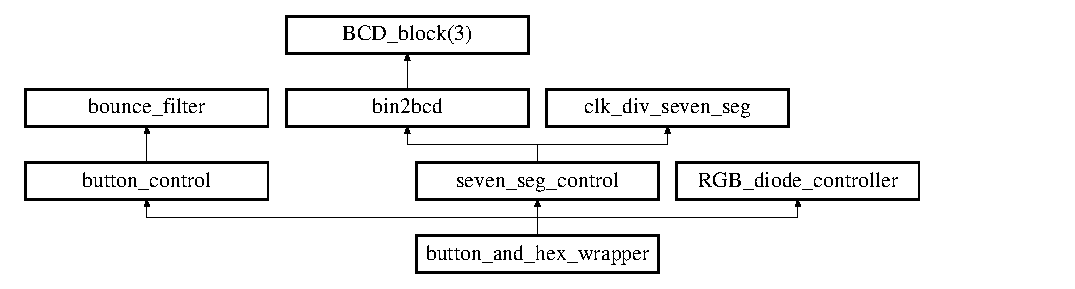
\includegraphics[height=3.435583cm]{classbutton__and__hex__wrapper}
\end{center}
\end{figure}
\subsection*{Entities}
\begin{DoxyCompactItemize}
\item 
\hyperlink{classbutton__and__hex__wrapper_1_1HID__wrapper}{H\-I\-D\-\_\-wrapper} architecture
\begin{DoxyCompactList}\small\item\em Architecture of the Dummy\-\_\-apb. \end{DoxyCompactList}\end{DoxyCompactItemize}
\subsection*{Libraries}
 \begin{DoxyCompactItemize}
\item 
\hypertarget{classbutton__and__hex__wrapper_ae4f03c286607f3181e16b9aa12d0c6d4}{\hyperlink{classbutton__and__hex__wrapper_ae4f03c286607f3181e16b9aa12d0c6d4}{I\-E\-E\-E} }\label{classbutton__and__hex__wrapper_ae4f03c286607f3181e16b9aa12d0c6d4}

\begin{DoxyCompactList}\small\item\em Use of standard library. \end{DoxyCompactList}\item 
\hypertarget{classbutton__and__hex__wrapper_a2306e6b22fb33ca087d2f1b289b10e28}{\hyperlink{classbutton__and__hex__wrapper_a2306e6b22fb33ca087d2f1b289b10e28}{grlib} }\label{classbutton__and__hex__wrapper_a2306e6b22fb33ca087d2f1b289b10e28}

\begin{DoxyCompactList}\small\item\em use of the G\-R\-L\-I\-B \end{DoxyCompactList}\end{DoxyCompactItemize}
\subsection*{Use Clauses}
 \begin{DoxyCompactItemize}
\item 
\hypertarget{classbutton__and__hex__wrapper_a68c233289eaf7d2601307bdd93b4c299}{\hyperlink{classbutton__and__hex__wrapper_a68c233289eaf7d2601307bdd93b4c299}{I\-E\-E\-E.\-S\-T\-D\-\_\-\-L\-O\-G\-I\-C\-\_\-1164.\-all}   }\label{classbutton__and__hex__wrapper_a68c233289eaf7d2601307bdd93b4c299}

\begin{DoxyCompactList}\small\item\em Use of standard logic arguments. \end{DoxyCompactList}\item 
\hypertarget{classbutton__and__hex__wrapper_a543ad46b77c6dc7048df8e72163d311d}{\hyperlink{classbutton__and__hex__wrapper_a543ad46b77c6dc7048df8e72163d311d}{grlib.\-amba.\-all}   }\label{classbutton__and__hex__wrapper_a543ad46b77c6dc7048df8e72163d311d}

\begin{DoxyCompactList}\small\item\em Use of the A\-M\-B\-A bus signals and constants. \end{DoxyCompactList}\item 
\hypertarget{classbutton__and__hex__wrapper_a8290b68c465332cd784781f7230e772d}{\hyperlink{classbutton__and__hex__wrapper_a8290b68c465332cd784781f7230e772d}{grlib.\-stdlib.\-all}   }\label{classbutton__and__hex__wrapper_a8290b68c465332cd784781f7230e772d}

\begin{DoxyCompactList}\small\item\em Use of standard G\-R\-L\-I\-B signals and constants. \end{DoxyCompactList}\item 
\hypertarget{classbutton__and__hex__wrapper_ad24672e694b1bed181a8b2813b132538}{\hyperlink{classbutton__and__hex__wrapper_ad24672e694b1bed181a8b2813b132538}{grlib.\-devices.\-all}   }\label{classbutton__and__hex__wrapper_ad24672e694b1bed181a8b2813b132538}

\begin{DoxyCompactList}\small\item\em use of G\-R\-L\-I\-B devices signals and constants \end{DoxyCompactList}\end{DoxyCompactItemize}
\subsection*{Generics}
 \begin{DoxyCompactItemize}
\item 
\hypertarget{classbutton__and__hex__wrapper_a5e1fd38c08cf4405b26bf887c5010e2b}{\hyperlink{classbutton__and__hex__wrapper_a5e1fd38c08cf4405b26bf887c5010e2b}{pindex} {\bfseries {\bfseries \textcolor{comment}{integer}\textcolor{vhdlchar}{ }\textcolor{vhdlchar}{\-:}\textcolor{vhdlchar}{=}\textcolor{vhdlchar}{ } \textcolor{vhdldigit}{0} \textcolor{vhdlchar}{ }}}}\label{classbutton__and__hex__wrapper_a5e1fd38c08cf4405b26bf887c5010e2b}

\begin{DoxyCompactList}\small\item\em Slave index. \end{DoxyCompactList}\item 
\hypertarget{classbutton__and__hex__wrapper_a1c4c90775fe1a0af1ff79546ceb2f9c2}{\hyperlink{classbutton__and__hex__wrapper_a1c4c90775fe1a0af1ff79546ceb2f9c2}{paddr} {\bfseries {\bfseries \textcolor{comment}{integer}\textcolor{vhdlchar}{ }\textcolor{vhdlchar}{\-:}\textcolor{vhdlchar}{=}\textcolor{vhdlchar}{ } \textcolor{vhdldigit}{0} \textcolor{vhdlchar}{ }}}}\label{classbutton__and__hex__wrapper_a1c4c90775fe1a0af1ff79546ceb2f9c2}

\begin{DoxyCompactList}\small\item\em Address of the A\-P\-B bank. \end{DoxyCompactList}\item 
\hypertarget{classbutton__and__hex__wrapper_a89dd0de36f24702f322479db69e5ff78}{\hyperlink{classbutton__and__hex__wrapper_a89dd0de36f24702f322479db69e5ff78}{pmask} {\bfseries {\bfseries \textcolor{comment}{integer}\textcolor{vhdlchar}{ }\textcolor{vhdlchar}{\-:}\textcolor{vhdlchar}{=}\textcolor{vhdlchar}{ } \textcolor{vhdldigit}{16\#002\#} \textcolor{vhdlchar}{ }}}}\label{classbutton__and__hex__wrapper_a89dd0de36f24702f322479db69e5ff78}

\begin{DoxyCompactList}\small\item\em Address range. \end{DoxyCompactList}\end{DoxyCompactItemize}
\subsection*{Ports}
 \begin{DoxyCompactItemize}
\item 
\hypertarget{classbutton__and__hex__wrapper_a8fb8388e1e2f3ac69332573f5909b4e8}{\hyperlink{classbutton__and__hex__wrapper_a8fb8388e1e2f3ac69332573f5909b4e8}{rstn}  {\bfseries {\bfseries \textcolor{vhdlkeyword}{in}\textcolor{vhdlchar}{ }}} {\bfseries \textcolor{comment}{std\-\_\-ulogic}\textcolor{vhdlchar}{ }} }\label{classbutton__and__hex__wrapper_a8fb8388e1e2f3ac69332573f5909b4e8}

\begin{DoxyCompactList}\small\item\em global reset, active low \end{DoxyCompactList}\item 
\hypertarget{classbutton__and__hex__wrapper_af1c59ef8e5ba3edeeb313b4be18d7d8a}{\hyperlink{classbutton__and__hex__wrapper_af1c59ef8e5ba3edeeb313b4be18d7d8a}{clk}  {\bfseries {\bfseries \textcolor{vhdlkeyword}{in}\textcolor{vhdlchar}{ }}} {\bfseries \textcolor{comment}{std\-\_\-ulogic}\textcolor{vhdlchar}{ }} }\label{classbutton__and__hex__wrapper_af1c59ef8e5ba3edeeb313b4be18d7d8a}

\begin{DoxyCompactList}\small\item\em Clock at the bus speed of 50 M\-Hz. \end{DoxyCompactList}\item 
\hypertarget{classbutton__and__hex__wrapper_abd7039100e504d8f92a35144147f07d7}{\hyperlink{classbutton__and__hex__wrapper_abd7039100e504d8f92a35144147f07d7}{apbi}  {\bfseries {\bfseries \textcolor{vhdlkeyword}{in}\textcolor{vhdlchar}{ }}} {\bfseries \textcolor{vhdlchar}{apb\-\_\-slv\-\_\-in\-\_\-type}\textcolor{vhdlchar}{ }} }\label{classbutton__and__hex__wrapper_abd7039100e504d8f92a35144147f07d7}

\begin{DoxyCompactList}\small\item\em A\-P\-B slave inputs. \end{DoxyCompactList}\item 
\hypertarget{classbutton__and__hex__wrapper_a7e895c34eed119599f289452433acbf2}{\hyperlink{classbutton__and__hex__wrapper_a7e895c34eed119599f289452433acbf2}{apbo}  {\bfseries {\bfseries \textcolor{vhdlkeyword}{out}\textcolor{vhdlchar}{ }}} {\bfseries \textcolor{vhdlchar}{apb\-\_\-slv\-\_\-out\-\_\-type}\textcolor{vhdlchar}{ }} }\label{classbutton__and__hex__wrapper_a7e895c34eed119599f289452433acbf2}

\begin{DoxyCompactList}\small\item\em A\-P\-B slave outputs. \end{DoxyCompactList}\item 
\hypertarget{classbutton__and__hex__wrapper_a72206c9efda7c958cf55b0a88cb0f12c}{\hyperlink{classbutton__and__hex__wrapper_a72206c9efda7c958cf55b0a88cb0f12c}{Buttons\-\_\-in}  {\bfseries {\bfseries \textcolor{vhdlkeyword}{in}\textcolor{vhdlchar}{ }}} {\bfseries \textcolor{comment}{S\-T\-D\-\_\-\-L\-O\-G\-I\-C\-\_\-\-V\-E\-C\-T\-O\-R}\textcolor{vhdlchar}{ }\textcolor{vhdlchar}{(}\textcolor{vhdlchar}{ }\textcolor{vhdlchar}{ } \textcolor{vhdldigit}{4} \textcolor{vhdlchar}{ }\textcolor{vhdlchar}{ }\textcolor{vhdlchar}{ }\textcolor{vhdlkeyword}{downto}\textcolor{vhdlchar}{ }\textcolor{vhdlchar}{ }\textcolor{vhdlchar}{ } \textcolor{vhdldigit}{0} \textcolor{vhdlchar}{ }\textcolor{vhdlchar}{)}\textcolor{vhdlchar}{ }} }\label{classbutton__and__hex__wrapper_a72206c9efda7c958cf55b0a88cb0f12c}

\begin{DoxyCompactList}\small\item\em Buttons in from the board. \end{DoxyCompactList}\item 
\hypertarget{classbutton__and__hex__wrapper_a45655c10fcad02d37d83f5279ebb199b}{\hyperlink{classbutton__and__hex__wrapper_a45655c10fcad02d37d83f5279ebb199b}{seven\-\_\-seg\-\_\-out}  {\bfseries {\bfseries \textcolor{vhdlkeyword}{out}\textcolor{vhdlchar}{ }}} {\bfseries \textcolor{comment}{S\-T\-D\-\_\-\-L\-O\-G\-I\-C\-\_\-\-V\-E\-C\-T\-O\-R}\textcolor{vhdlchar}{ }\textcolor{vhdlchar}{(}\textcolor{vhdlchar}{ }\textcolor{vhdlchar}{ } \textcolor{vhdldigit}{6} \textcolor{vhdlchar}{ }\textcolor{vhdlchar}{ }\textcolor{vhdlchar}{ }\textcolor{vhdlkeyword}{downto}\textcolor{vhdlchar}{ }\textcolor{vhdlchar}{ }\textcolor{vhdlchar}{ } \textcolor{vhdldigit}{0} \textcolor{vhdlchar}{ }\textcolor{vhdlchar}{)}\textcolor{vhdlchar}{ }} }\label{classbutton__and__hex__wrapper_a45655c10fcad02d37d83f5279ebb199b}

\begin{DoxyCompactList}\small\item\em Seven\-\_\-sel\-\_\-out marks the seven segment display of the current selected seven segment display segment. \end{DoxyCompactList}\item 
\hypertarget{classbutton__and__hex__wrapper_ae1646bd2ce2b0e1d1bb85bf2a88d1b5f}{\hyperlink{classbutton__and__hex__wrapper_ae1646bd2ce2b0e1d1bb85bf2a88d1b5f}{seven\-\_\-seg\-\_\-sel}  {\bfseries {\bfseries \textcolor{vhdlkeyword}{out}\textcolor{vhdlchar}{ }}} {\bfseries \textcolor{comment}{S\-T\-D\-\_\-\-L\-O\-G\-I\-C\-\_\-\-V\-E\-C\-T\-O\-R}\textcolor{vhdlchar}{ }\textcolor{vhdlchar}{(}\textcolor{vhdlchar}{ }\textcolor{vhdlchar}{ } \textcolor{vhdldigit}{7} \textcolor{vhdlchar}{ }\textcolor{vhdlchar}{ }\textcolor{vhdlchar}{ }\textcolor{vhdlkeyword}{downto}\textcolor{vhdlchar}{ }\textcolor{vhdlchar}{ }\textcolor{vhdlchar}{ } \textcolor{vhdldigit}{0} \textcolor{vhdlchar}{ }\textcolor{vhdlchar}{)}\textcolor{vhdlchar}{ }} }\label{classbutton__and__hex__wrapper_ae1646bd2ce2b0e1d1bb85bf2a88d1b5f}

\begin{DoxyCompactList}\small\item\em Seven\-\_\-seg\-\_\-sel marks the current selected seven segment display. \end{DoxyCompactList}\item 
\hypertarget{classbutton__and__hex__wrapper_a7691db71e3330cb4b875bb27e8fbb8c7}{\hyperlink{classbutton__and__hex__wrapper_a7691db71e3330cb4b875bb27e8fbb8c7}{diode\-\_\-out}  {\bfseries {\bfseries \textcolor{vhdlkeyword}{out}\textcolor{vhdlchar}{ }}} {\bfseries \textcolor{comment}{S\-T\-D\-\_\-\-L\-O\-G\-I\-C\-\_\-vector}\textcolor{vhdlchar}{ }\textcolor{vhdlchar}{(}\textcolor{vhdlchar}{ }\textcolor{vhdlchar}{ } \textcolor{vhdldigit}{2} \textcolor{vhdlchar}{ }\textcolor{vhdlchar}{ }\textcolor{vhdlchar}{ }\textcolor{vhdlkeyword}{downto}\textcolor{vhdlchar}{ }\textcolor{vhdlchar}{ }\textcolor{vhdlchar}{ } \textcolor{vhdldigit}{0} \textcolor{vhdlchar}{ }\textcolor{vhdlchar}{)}\textcolor{vhdlchar}{ }} }\label{classbutton__and__hex__wrapper_a7691db71e3330cb4b875bb27e8fbb8c7}

\begin{DoxyCompactList}\small\item\em diode\-\_\-out is a vector containing the state of the red, green and blue diode \end{DoxyCompactList}\end{DoxyCompactItemize}


\subsection{Detailed Description}
This component gathers all the sub-\/modules needed for H\-I\-D. It also supplies an interface to the A\-P\-B bus. 

The documentation for this class was generated from the following file\-:\begin{DoxyCompactItemize}
\item 
\hyperlink{Button__and__hex__wrapper_8vhd}{Button\-\_\-and\-\_\-hex\-\_\-wrapper.\-vhd}\end{DoxyCompactItemize}

\hypertarget{classbutton__control}{\section{button\-\_\-control Entity Reference}
\label{classbutton__control}\index{button\-\_\-control@{button\-\_\-control}}
}
Inheritance diagram for button\-\_\-control\-:\begin{figure}[H]
\begin{center}
\leavevmode
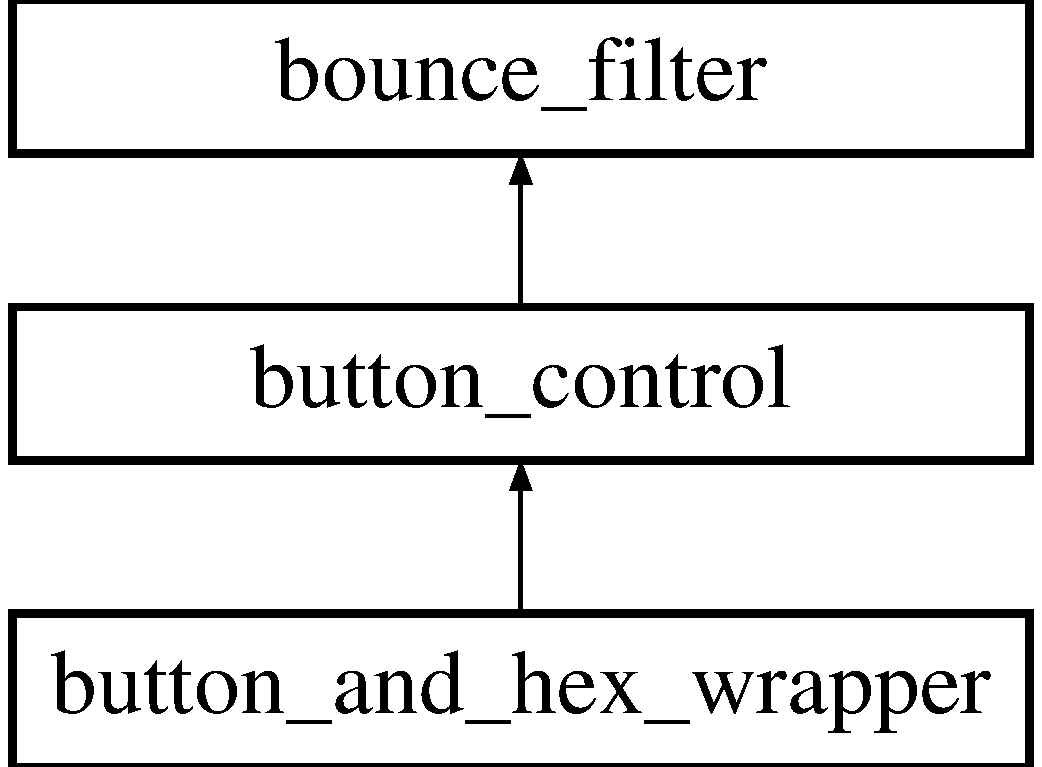
\includegraphics[height=3.000000cm]{classbutton__control}
\end{center}
\end{figure}
\subsection*{Entities}
\begin{DoxyCompactItemize}
\item 
\hyperlink{classbutton__control_1_1control__button}{control\-\_\-button} architecture
\begin{DoxyCompactList}\small\item\em Architecture of the \hyperlink{classbutton__control}{button\-\_\-control}. \end{DoxyCompactList}\end{DoxyCompactItemize}
\subsection*{Libraries}
 \begin{DoxyCompactItemize}
\item 
\hypertarget{classbutton__control_ae4f03c286607f3181e16b9aa12d0c6d4}{\hyperlink{classbutton__control_ae4f03c286607f3181e16b9aa12d0c6d4}{I\-E\-E\-E} }\label{classbutton__control_ae4f03c286607f3181e16b9aa12d0c6d4}

\begin{DoxyCompactList}\small\item\em Use of standard library. \end{DoxyCompactList}\end{DoxyCompactItemize}
\subsection*{Use Clauses}
 \begin{DoxyCompactItemize}
\item 
\hypertarget{classbutton__control_a68c233289eaf7d2601307bdd93b4c299}{\hyperlink{classbutton__control_a68c233289eaf7d2601307bdd93b4c299}{I\-E\-E\-E.\-S\-T\-D\-\_\-\-L\-O\-G\-I\-C\-\_\-1164.\-all}   }\label{classbutton__control_a68c233289eaf7d2601307bdd93b4c299}

\begin{DoxyCompactList}\small\item\em Use of standard logic arguments. \end{DoxyCompactList}\item 
\hypertarget{classbutton__control_a7c135c43c66ccd7f22abe5f6211788a5}{\hyperlink{classbutton__control_a7c135c43c66ccd7f22abe5f6211788a5}{I\-E\-E\-E.\-N\-U\-M\-E\-R\-I\-C\-\_\-\-S\-T\-D.\-all}   }\label{classbutton__control_a7c135c43c66ccd7f22abe5f6211788a5}

\begin{DoxyCompactList}\small\item\em Use of standard numerical arguments. \end{DoxyCompactList}\end{DoxyCompactItemize}
\subsection*{Ports}
 \begin{DoxyCompactItemize}
\item 
\hypertarget{classbutton__control_a8120037e0ee47c35ba2d79242209c72e}{\hyperlink{classbutton__control_a8120037e0ee47c35ba2d79242209c72e}{clk}  {\bfseries {\bfseries \textcolor{vhdlkeyword}{in}\textcolor{vhdlchar}{ }}} {\bfseries \textcolor{comment}{S\-T\-D\-\_\-\-L\-O\-G\-I\-C}\textcolor{vhdlchar}{ }} }\label{classbutton__control_a8120037e0ee47c35ba2d79242209c72e}

\begin{DoxyCompactList}\small\item\em Clock in for registers. \end{DoxyCompactList}\item 
\hypertarget{classbutton__control_aba021aec4b477b89079bb58ccadcc67e}{\hyperlink{classbutton__control_aba021aec4b477b89079bb58ccadcc67e}{rstn}  {\bfseries {\bfseries \textcolor{vhdlkeyword}{in}\textcolor{vhdlchar}{ }}} {\bfseries \textcolor{comment}{S\-T\-D\-\_\-\-L\-O\-G\-I\-C}\textcolor{vhdlchar}{ }} }\label{classbutton__control_aba021aec4b477b89079bb58ccadcc67e}

\begin{DoxyCompactList}\small\item\em Global reset, active low. \end{DoxyCompactList}\item 
\hypertarget{classbutton__control_a7767950aafd1dd8ca4b5c572d49dfdff}{\hyperlink{classbutton__control_a7767950aafd1dd8ca4b5c572d49dfdff}{buttons\-\_\-in}  {\bfseries {\bfseries \textcolor{vhdlkeyword}{in}\textcolor{vhdlchar}{ }}} {\bfseries \textcolor{comment}{S\-T\-D\-\_\-\-L\-O\-G\-I\-C\-\_\-\-V\-E\-C\-T\-O\-R}\textcolor{vhdlchar}{ }\textcolor{vhdlchar}{(}\textcolor{vhdlchar}{ }\textcolor{vhdlchar}{ } \textcolor{vhdldigit}{4} \textcolor{vhdlchar}{ }\textcolor{vhdlchar}{ }\textcolor{vhdlchar}{ }\textcolor{vhdlkeyword}{downto}\textcolor{vhdlchar}{ }\textcolor{vhdlchar}{ }\textcolor{vhdlchar}{ } \textcolor{vhdldigit}{0} \textcolor{vhdlchar}{ }\textcolor{vhdlchar}{)}\textcolor{vhdlchar}{ }} }\label{classbutton__control_a7767950aafd1dd8ca4b5c572d49dfdff}

\begin{DoxyCompactList}\small\item\em Buttons in. \end{DoxyCompactList}\item 
\hypertarget{classbutton__control_aa730ff47d713456d7cf31891ba98fbfd}{\hyperlink{classbutton__control_aa730ff47d713456d7cf31891ba98fbfd}{current\-\_\-preset}  {\bfseries {\bfseries \textcolor{vhdlkeyword}{out}\textcolor{vhdlchar}{ }}} {\bfseries \textcolor{comment}{S\-T\-D\-\_\-\-L\-O\-G\-I\-C\-\_\-\-V\-E\-C\-T\-O\-R}\textcolor{vhdlchar}{ }\textcolor{vhdlchar}{(}\textcolor{vhdlchar}{ }\textcolor{vhdlchar}{ } \textcolor{vhdldigit}{7} \textcolor{vhdlchar}{ }\textcolor{vhdlchar}{ }\textcolor{vhdlchar}{ }\textcolor{vhdlkeyword}{downto}\textcolor{vhdlchar}{ }\textcolor{vhdlchar}{ }\textcolor{vhdlchar}{ } \textcolor{vhdldigit}{0} \textcolor{vhdlchar}{ }\textcolor{vhdlchar}{)}\textcolor{vhdlchar}{ }} }\label{classbutton__control_aa730ff47d713456d7cf31891ba98fbfd}

\begin{DoxyCompactList}\small\item\em Current value out. \end{DoxyCompactList}\item 
\hypertarget{classbutton__control_acae3f7008d8aaf35bca56c9b3e56df11}{\hyperlink{classbutton__control_acae3f7008d8aaf35bca56c9b3e56df11}{selected\-\_\-preset}  {\bfseries {\bfseries \textcolor{vhdlkeyword}{out}\textcolor{vhdlchar}{ }}} {\bfseries \textcolor{comment}{S\-T\-D\-\_\-\-L\-O\-G\-I\-C\-\_\-\-V\-E\-C\-T\-O\-R}\textcolor{vhdlchar}{ }\textcolor{vhdlchar}{(}\textcolor{vhdlchar}{ }\textcolor{vhdlchar}{ } \textcolor{vhdldigit}{7} \textcolor{vhdlchar}{ }\textcolor{vhdlchar}{ }\textcolor{vhdlchar}{ }\textcolor{vhdlkeyword}{downto}\textcolor{vhdlchar}{ }\textcolor{vhdlchar}{ }\textcolor{vhdlchar}{ } \textcolor{vhdldigit}{0} \textcolor{vhdlchar}{ }\textcolor{vhdlchar}{)}\textcolor{vhdlchar}{ }} }\label{classbutton__control_acae3f7008d8aaf35bca56c9b3e56df11}

\begin{DoxyCompactList}\small\item\em Selected value out. \end{DoxyCompactList}\item 
\hypertarget{classbutton__control_ab89db7a1fc99970f775fa8768438db8a}{\hyperlink{classbutton__control_ab89db7a1fc99970f775fa8768438db8a}{read\-\_\-interupt}  {\bfseries {\bfseries \textcolor{vhdlkeyword}{out}\textcolor{vhdlchar}{ }}} {\bfseries \textcolor{comment}{S\-T\-D\-\_\-\-L\-O\-G\-I\-C}\textcolor{vhdlchar}{ }} }\label{classbutton__control_ab89db7a1fc99970f775fa8768438db8a}

\begin{DoxyCompactList}\small\item\em Interrupt indicating a read from flash is to be done. \end{DoxyCompactList}\item 
\hypertarget{classbutton__control_a976537540918c28b4b20479c41d03ac8}{\hyperlink{classbutton__control_a976537540918c28b4b20479c41d03ac8}{write\-\_\-interupt}  {\bfseries {\bfseries \textcolor{vhdlkeyword}{out}\textcolor{vhdlchar}{ }}} {\bfseries \textcolor{comment}{S\-T\-D\-\_\-\-L\-O\-G\-I\-C}\textcolor{vhdlchar}{ }} }\label{classbutton__control_a976537540918c28b4b20479c41d03ac8}

\begin{DoxyCompactList}\small\item\em Interrupt indicating a write to flash is to be done. \end{DoxyCompactList}\end{DoxyCompactItemize}


The documentation for this class was generated from the following file\-:\begin{DoxyCompactItemize}
\item 
\hyperlink{button__control_8vhd}{button\-\_\-control.\-vhd}\end{DoxyCompactItemize}

\hypertarget{classclk__divide_1_1clk__div__DAC}{\section{clk\-\_\-div\-\_\-\-D\-A\-C Architecture Reference}
\label{classclk__divide_1_1clk__div__DAC}\index{clk\-\_\-div\-\_\-\-D\-A\-C@{clk\-\_\-div\-\_\-\-D\-A\-C}}
}


Architecture of the clk\-\_\-divider.  


\subsection*{Processes}
 \begin{DoxyCompactItemize}
\item 
\hypertarget{classclk__divide_1_1clk__div__DAC_aae31a4dbedaf43cbd1619c642270813b}{\hyperlink{classclk__divide_1_1clk__div__DAC_aae31a4dbedaf43cbd1619c642270813b}{P\-R\-O\-C\-E\-S\-S\-\_\-5}{\bfseries  ( {\bfseries {\bfseries \hyperlink{classclk__divide_a8120037e0ee47c35ba2d79242209c72e}{clk}} \textcolor{vhdlchar}{ }\textcolor{vhdlchar}{ }\textcolor{vhdlchar}{ }} , {\bfseries {\bfseries \hyperlink{classclk__divide_aa7b7040844189161771c36cf6bbf172c}{rst}} \textcolor{vhdlchar}{ }} )}}\label{classclk__divide_1_1clk__div__DAC_aae31a4dbedaf43cbd1619c642270813b}

\begin{DoxyCompactList}\small\item\em When the system is reseted all values are set to 0. \end{DoxyCompactList}\end{DoxyCompactItemize}
\subsection*{Constants}
 \begin{DoxyCompactItemize}
\item 
\hypertarget{classclk__divide_1_1clk__div__DAC_a8f64c0dba167ef17ec71f04787ff5a8a}{\hyperlink{classclk__divide_1_1clk__div__DAC_a8f64c0dba167ef17ec71f04787ff5a8a}{cnt44k\-Hz\-\_\-max} {\bfseries \textcolor{comment}{integer}\textcolor{vhdlchar}{ }\textcolor{vhdlchar}{ }\textcolor{vhdlchar}{\-:}\textcolor{vhdlchar}{=}\textcolor{vhdlchar}{ }\textcolor{comment}{integer}\textcolor{vhdlchar}{ }\textcolor{vhdlchar}{(}\textcolor{vhdlchar}{ }\textcolor{vhdlchar}{ }\textcolor{vhdlchar}{round}\textcolor{vhdlchar}{ }\textcolor{vhdlchar}{(}\textcolor{vhdlchar}{ }\textcolor{vhdlchar}{ }\textcolor{comment}{real}\textcolor{vhdlchar}{ }\textcolor{vhdlchar}{(}\textcolor{vhdlchar}{ }\textcolor{vhdlchar}{ }{\bfseries \hyperlink{classclk__divide_a81d31886de4b5afc05873543265dcf7c}{systemclock}} \textcolor{vhdlchar}{ }\textcolor{vhdlchar}{)}\textcolor{vhdlchar}{ }\textcolor{vhdlchar}{ }\textcolor{vhdlchar}{/}\textcolor{vhdlchar}{ }\textcolor{comment}{real}\textcolor{vhdlchar}{ }\textcolor{vhdlchar}{(}\textcolor{vhdlchar}{ }\textcolor{vhdlchar}{ }\textcolor{vhdlchar}{(}\textcolor{vhdlchar}{ }{\bfseries \hyperlink{classclk__divide_a046b87df8ce0a99f5bacf19e5027cccf}{sampleclock}} \textcolor{vhdlchar}{ }\textcolor{vhdlchar}{$\ast$}\textcolor{vhdlchar}{ }{\bfseries \hyperlink{classclk__divide_aeab4f828c7bc0927792f6a9c6bf1b63f}{O\-S\-R}} \textcolor{vhdlchar}{ }\textcolor{vhdlchar}{)}\textcolor{vhdlchar}{ }\textcolor{vhdlchar}{ }\textcolor{vhdlchar}{)}\textcolor{vhdlchar}{ }\textcolor{vhdlchar}{ }\textcolor{vhdlchar}{)}\textcolor{vhdlchar}{ }\textcolor{vhdlchar}{ }\textcolor{vhdlchar}{)}\textcolor{vhdlchar}{ }\textcolor{vhdlchar}{ }\textcolor{vhdlchar}{$\ast$}\textcolor{vhdlchar}{ }{\bfseries \hyperlink{classclk__divide_aeab4f828c7bc0927792f6a9c6bf1b63f}{O\-S\-R}} \textcolor{vhdlchar}{ }\textcolor{vhdlchar}{-\/}\textcolor{vhdlchar}{ }} }\label{classclk__divide_1_1clk__div__DAC_a8f64c0dba167ef17ec71f04787ff5a8a}

\begin{DoxyCompactList}\small\item\em The cnt44k\-Hz max calculates the number the counter has to reach to reset. The calculation is as follows\-: \$round(\{systemclock\}\{sampleclock$\ast$\-O\-S\-R\})$\ast$\-O\-R\-S-\/1. The O\-S\-R is in the equation to make sure the rate between sample clock and O\-S\-R will be correct. \end{DoxyCompactList}\end{DoxyCompactItemize}
\subsection*{Signals}
 \begin{DoxyCompactItemize}
\item 
\hypertarget{classclk__divide_1_1clk__div__DAC_a119377ea25e90c9e0302742fb8d75456}{\hyperlink{classclk__divide_1_1clk__div__DAC_a119377ea25e90c9e0302742fb8d75456}{cnt44k\-Hz} {\bfseries \textcolor{comment}{integer}\textcolor{vhdlchar}{ }\textcolor{vhdlkeyword}{range}\textcolor{vhdlchar}{ } \textcolor{vhdldigit}{0} \textcolor{vhdlchar}{ }\textcolor{vhdlchar}{ }\textcolor{vhdlchar}{ }\textcolor{vhdlkeyword}{to}\textcolor{vhdlchar}{ }\textcolor{vhdlchar}{ }\textcolor{vhdlchar}{ }{\bfseries \hyperlink{classclk__divide_1_1clk__div__DAC_a8f64c0dba167ef17ec71f04787ff5a8a}{cnt44k\-Hz\-\_\-max}} \textcolor{vhdlchar}{ }} }\label{classclk__divide_1_1clk__div__DAC_a119377ea25e90c9e0302742fb8d75456}

\begin{DoxyCompactList}\small\item\em Counter signal with the required range. \end{DoxyCompactList}\item 
\hypertarget{classclk__divide_1_1clk__div__DAC_ab62cba3781d0056853b0d98ca65ea351}{\hyperlink{classclk__divide_1_1clk__div__DAC_ab62cba3781d0056853b0d98ca65ea351}{clk50\-M\-Hzbuf} {\bfseries \textcolor{comment}{S\-T\-D\-\_\-\-L\-O\-G\-I\-C}\textcolor{vhdlchar}{ }} }\label{classclk__divide_1_1clk__div__DAC_ab62cba3781d0056853b0d98ca65ea351}

\begin{DoxyCompactList}\small\item\em Buffered value for the 50 M\-Hz clock to be able to use their states for calculation. \end{DoxyCompactList}\item 
\hypertarget{classclk__divide_1_1clk__div__DAC_aaa88cd1782ca3c642feace13266e5f9f}{\hyperlink{classclk__divide_1_1clk__div__DAC_aaa88cd1782ca3c642feace13266e5f9f}{clk25\-M\-Hzbuf} {\bfseries \textcolor{comment}{S\-T\-D\-\_\-\-L\-O\-G\-I\-C}\textcolor{vhdlchar}{ }} }\label{classclk__divide_1_1clk__div__DAC_aaa88cd1782ca3c642feace13266e5f9f}

\begin{DoxyCompactList}\small\item\em Buffered value for the 25 M\-Hz clock to be able to use their states for calculation. \end{DoxyCompactList}\item 
\hypertarget{classclk__divide_1_1clk__div__DAC_a4b92d2406ba07f6283fa1d9ad64e472d}{\hyperlink{classclk__divide_1_1clk__div__DAC_a4b92d2406ba07f6283fa1d9ad64e472d}{clk44k\-Hzbuf} {\bfseries \textcolor{comment}{S\-T\-D\-\_\-\-L\-O\-G\-I\-C}\textcolor{vhdlchar}{ }} }\label{classclk__divide_1_1clk__div__DAC_a4b92d2406ba07f6283fa1d9ad64e472d}

\begin{DoxyCompactList}\small\item\em Buffered value for the 44 k\-Hz clock to be able to use their states for calculation. \end{DoxyCompactList}\item 
\hypertarget{classclk__divide_1_1clk__div__DAC_a7683c8432ba1dc0ce9ac4515e56c9d4f}{\hyperlink{classclk__divide_1_1clk__div__DAC_a7683c8432ba1dc0ce9ac4515e56c9d4f}{clk705k\-Hzbuf} {\bfseries \textcolor{comment}{S\-T\-D\-\_\-\-L\-O\-G\-I\-C}\textcolor{vhdlchar}{ }} }\label{classclk__divide_1_1clk__div__DAC_a7683c8432ba1dc0ce9ac4515e56c9d4f}

\begin{DoxyCompactList}\small\item\em Buffered value for the 705 k\-Hz clock to be able to use their states for calculation. \end{DoxyCompactList}\end{DoxyCompactItemize}


\subsection{Detailed Description}
Architecture of the clk\-\_\-divider. 

The architecture containing the main body of the component. 

The documentation for this class was generated from the following file\-:\begin{DoxyCompactItemize}
\item 
\hyperlink{CLK__divide_8vhd}{C\-L\-K\-\_\-divide.\-vhd}\end{DoxyCompactItemize}

\hypertarget{classclk__div__seven__seg_1_1clk__div__seven}{\section{clk\-\_\-div\-\_\-seven Architecture Reference}
\label{classclk__div__seven__seg_1_1clk__div__seven}\index{clk\-\_\-div\-\_\-seven@{clk\-\_\-div\-\_\-seven}}
}


Architecture of the \hyperlink{classclk__div__seven__seg}{clk\-\_\-div\-\_\-seven\-\_\-seg}.  


\subsection*{Processes}
 \begin{DoxyCompactItemize}
\item 
\hypertarget{classclk__div__seven__seg_1_1clk__div__seven_afbf5b75c435428d734b3dd7d2f63b351}{\hyperlink{classclk__div__seven__seg_1_1clk__div__seven_afbf5b75c435428d734b3dd7d2f63b351}{P\-R\-O\-C\-E\-S\-S\-\_\-4}{\bfseries  ( {\bfseries {\bfseries \hyperlink{classclk__div__seven__seg_aba021aec4b477b89079bb58ccadcc67e}{rstn}} \textcolor{vhdlchar}{ }\textcolor{vhdlchar}{ }\textcolor{vhdlchar}{ }} , {\bfseries {\bfseries \hyperlink{classclk__div__seven__seg_a8120037e0ee47c35ba2d79242209c72e}{clk}} \textcolor{vhdlchar}{ }} )}}\label{classclk__div__seven__seg_1_1clk__div__seven_afbf5b75c435428d734b3dd7d2f63b351}

\end{DoxyCompactItemize}
\subsection*{Signals}
 \begin{DoxyCompactItemize}
\item 
\hypertarget{classclk__div__seven__seg_1_1clk__div__seven_ac4dba71b323197d34acd6eeed07686d6}{\hyperlink{classclk__div__seven__seg_1_1clk__div__seven_ac4dba71b323197d34acd6eeed07686d6}{cnt} {\bfseries \textcolor{comment}{integer}\textcolor{vhdlchar}{ }\textcolor{vhdlkeyword}{range}\textcolor{vhdlchar}{ } \textcolor{vhdldigit}{0} \textcolor{vhdlchar}{ }\textcolor{vhdlchar}{ }\textcolor{vhdlchar}{ }\textcolor{vhdlkeyword}{to}\textcolor{vhdlchar}{ }\textcolor{vhdlchar}{ }\textcolor{vhdlchar}{ } \textcolor{vhdldigit}{2} \textcolor{vhdlchar}{ }\textcolor{vhdlchar}{$\ast$}\textcolor{vhdlchar}{$\ast$}\textcolor{vhdlchar}{ }{\bfseries \hyperlink{classclk__div__seven__seg_a8e97268cd0d50c552668e2c1d8719c2c}{counterbits}} \textcolor{vhdlchar}{ }\textcolor{vhdlchar}{-\/}\textcolor{vhdlchar}{ } \textcolor{vhdldigit}{1} \textcolor{vhdlchar}{ }} }\label{classclk__div__seven__seg_1_1clk__div__seven_ac4dba71b323197d34acd6eeed07686d6}

\begin{DoxyCompactList}\small\item\em The counter. \end{DoxyCompactList}\end{DoxyCompactItemize}


\subsection{Detailed Description}
Architecture of the \hyperlink{classclk__div__seven__seg}{clk\-\_\-div\-\_\-seven\-\_\-seg}. 

This clock divider is need to make sure seven segments of the seven segment displays in the correct speed. To fast and numbers will \char`\"{}float\char`\"{} to its neighbors due to slow transients, to slow and the numbers will appear as flashing instead of solid. 

The documentation for this class was generated from the following file\-:\begin{DoxyCompactItemize}
\item 
\hyperlink{clk__div__seven__seg_8vhd}{clk\-\_\-div\-\_\-seven\-\_\-seg.\-vhd}\end{DoxyCompactItemize}

\hypertarget{classclk__div__seven__seg}{\section{clk\-\_\-div\-\_\-seven\-\_\-seg Entity Reference}
\label{classclk__div__seven__seg}\index{clk\-\_\-div\-\_\-seven\-\_\-seg@{clk\-\_\-div\-\_\-seven\-\_\-seg}}
}


This component takes the system clock divides it for Seven segment displays. This is done by implementing counters.  


Inheritance diagram for clk\-\_\-div\-\_\-seven\-\_\-seg\-:\begin{figure}[H]
\begin{center}
\leavevmode
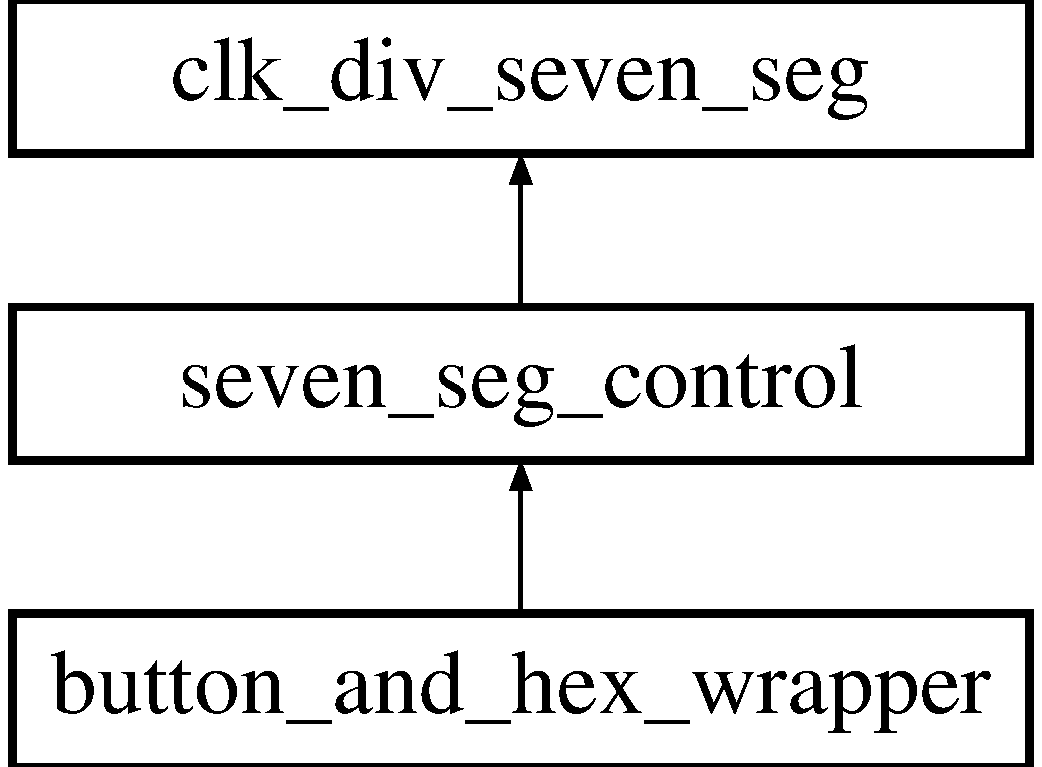
\includegraphics[height=3.000000cm]{classclk__div__seven__seg}
\end{center}
\end{figure}
\subsection*{Entities}
\begin{DoxyCompactItemize}
\item 
\hyperlink{classclk__div__seven__seg_1_1Behavioral}{Behavioral} architecture
\begin{DoxyCompactList}\small\item\em Architecture of the \hyperlink{classclk__div__seven__seg}{clk\-\_\-div\-\_\-seven\-\_\-seg}. \end{DoxyCompactList}\end{DoxyCompactItemize}
\subsection*{Libraries}
 \begin{DoxyCompactItemize}
\item 
\hypertarget{classclk__div__seven__seg_ae4f03c286607f3181e16b9aa12d0c6d4}{\hyperlink{classclk__div__seven__seg_ae4f03c286607f3181e16b9aa12d0c6d4}{I\-E\-E\-E} }\label{classclk__div__seven__seg_ae4f03c286607f3181e16b9aa12d0c6d4}

\begin{DoxyCompactList}\small\item\em Use of standard library. \end{DoxyCompactList}\end{DoxyCompactItemize}
\subsection*{Use Clauses}
 \begin{DoxyCompactItemize}
\item 
\hypertarget{classclk__div__seven__seg_a68c233289eaf7d2601307bdd93b4c299}{\hyperlink{classclk__div__seven__seg_a68c233289eaf7d2601307bdd93b4c299}{I\-E\-E\-E.\-S\-T\-D\-\_\-\-L\-O\-G\-I\-C\-\_\-1164.\-all}   }\label{classclk__div__seven__seg_a68c233289eaf7d2601307bdd93b4c299}

\begin{DoxyCompactList}\small\item\em Use of standard logic arguments. \end{DoxyCompactList}\item 
\hypertarget{classclk__div__seven__seg_a7c135c43c66ccd7f22abe5f6211788a5}{\hyperlink{classclk__div__seven__seg_a7c135c43c66ccd7f22abe5f6211788a5}{I\-E\-E\-E.\-N\-U\-M\-E\-R\-I\-C\-\_\-\-S\-T\-D.\-all}   }\label{classclk__div__seven__seg_a7c135c43c66ccd7f22abe5f6211788a5}

\begin{DoxyCompactList}\small\item\em Use of standard numerical arguments. \end{DoxyCompactList}\end{DoxyCompactItemize}
\subsection*{Generics}
 \begin{DoxyCompactItemize}
\item 
\hypertarget{classclk__div__seven__seg_a8e97268cd0d50c552668e2c1d8719c2c}{\hyperlink{classclk__div__seven__seg_a8e97268cd0d50c552668e2c1d8719c2c}{counterbits} {\bfseries {\bfseries \textcolor{comment}{integer}\textcolor{vhdlchar}{ }\textcolor{vhdlchar}{\-:}\textcolor{vhdlchar}{=}\textcolor{vhdlchar}{ } \textcolor{vhdldigit}{17} \textcolor{vhdlchar}{ }}}}\label{classclk__div__seven__seg_a8e97268cd0d50c552668e2c1d8719c2c}

\begin{DoxyCompactList}\small\item\em A generic for setting the bits of the counter. \end{DoxyCompactList}\end{DoxyCompactItemize}
\subsection*{Ports}
 \begin{DoxyCompactItemize}
\item 
\hypertarget{classclk__div__seven__seg_a8120037e0ee47c35ba2d79242209c72e}{\hyperlink{classclk__div__seven__seg_a8120037e0ee47c35ba2d79242209c72e}{clk}  {\bfseries {\bfseries \textcolor{vhdlkeyword}{in}\textcolor{vhdlchar}{ }}} {\bfseries \textcolor{comment}{S\-T\-D\-\_\-\-L\-O\-G\-I\-C}\textcolor{vhdlchar}{ }} }\label{classclk__div__seven__seg_a8120037e0ee47c35ba2d79242209c72e}

\begin{DoxyCompactList}\small\item\em Clock for counter and registers. \end{DoxyCompactList}\item 
\hypertarget{classclk__div__seven__seg_aba021aec4b477b89079bb58ccadcc67e}{\hyperlink{classclk__div__seven__seg_aba021aec4b477b89079bb58ccadcc67e}{rstn}  {\bfseries {\bfseries \textcolor{vhdlkeyword}{in}\textcolor{vhdlchar}{ }}} {\bfseries \textcolor{comment}{S\-T\-D\-\_\-\-L\-O\-G\-I\-C}\textcolor{vhdlchar}{ }} }\label{classclk__div__seven__seg_aba021aec4b477b89079bb58ccadcc67e}

\begin{DoxyCompactList}\small\item\em Global reset, active low. \end{DoxyCompactList}\item 
\hypertarget{classclk__div__seven__seg_a222a9878f2d09833d2a12c83c451bbd4}{\hyperlink{classclk__div__seven__seg_a222a9878f2d09833d2a12c83c451bbd4}{slow\-\_\-clk}  {\bfseries {\bfseries \textcolor{vhdlkeyword}{out}\textcolor{vhdlchar}{ }}} {\bfseries \textcolor{comment}{S\-T\-D\-\_\-\-L\-O\-G\-I\-C}\textcolor{vhdlchar}{ }} }\label{classclk__div__seven__seg_a222a9878f2d09833d2a12c83c451bbd4}

\begin{DoxyCompactList}\small\item\em The output slower clock. \end{DoxyCompactList}\end{DoxyCompactItemize}


\subsection{Detailed Description}
This component takes the system clock divides it for Seven segment displays. This is done by implementing counters. 

The documentation for this class was generated from the following file\-:\begin{DoxyCompactItemize}
\item 
\hyperlink{clk__div__seven__seg_8vhd}{clk\-\_\-div\-\_\-seven\-\_\-seg.\-vhd}\end{DoxyCompactItemize}

\hypertarget{classclk__divide}{\section{clk\-\_\-divide Entity Reference}
\label{classclk__divide}\index{clk\-\_\-divide@{clk\-\_\-divide}}
}


This component takes the system clock divides it for A\-D\-C/\-D\-A\-C components using lower clocks. This is done by implementing counters. When a certain counter reached a set number it will change the output and reset the counter.  


Inheritance diagram for clk\-\_\-divide\-:\begin{figure}[H]
\begin{center}
\leavevmode
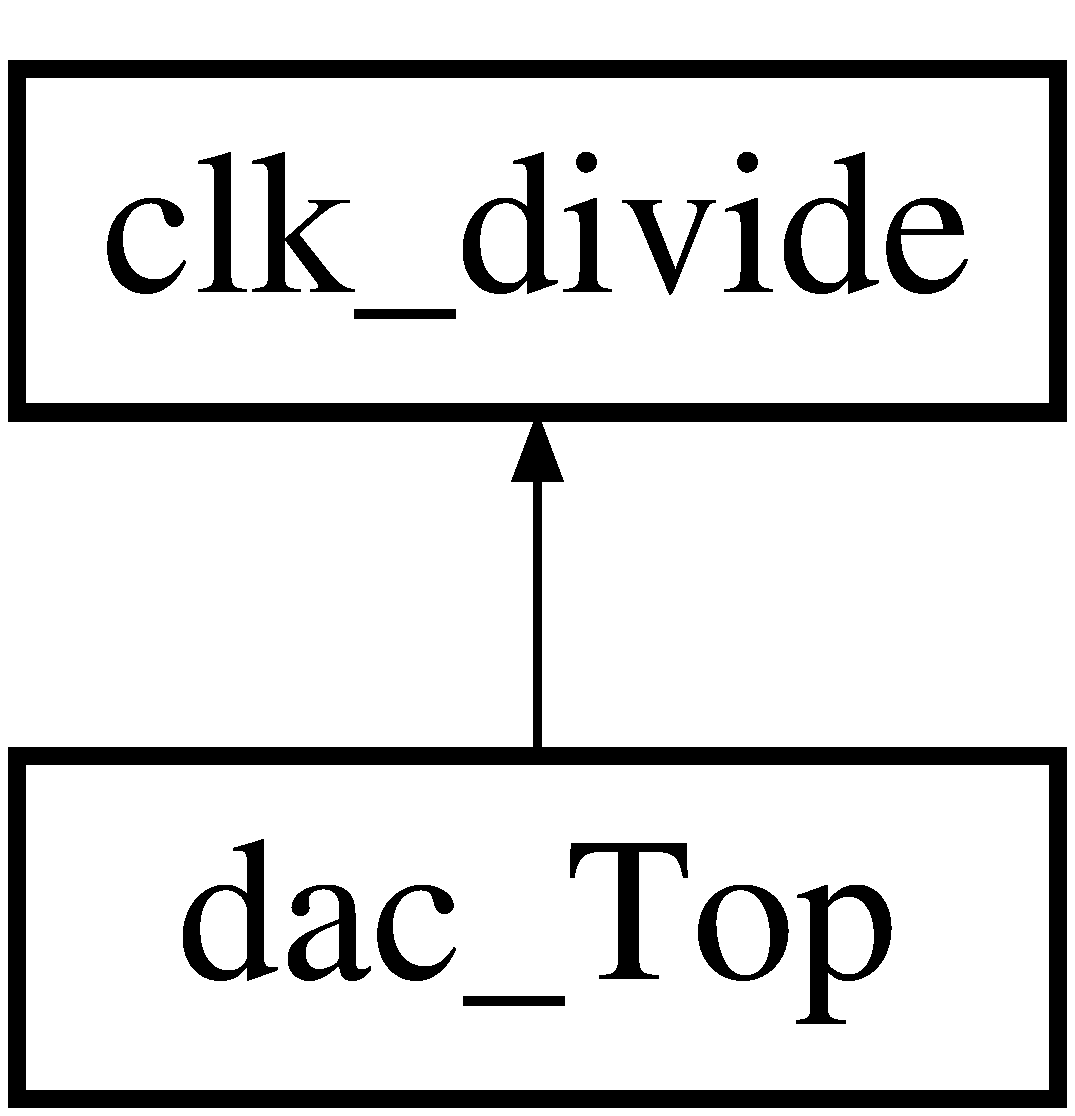
\includegraphics[height=2.000000cm]{classclk__divide}
\end{center}
\end{figure}
\subsection*{Entities}
\begin{DoxyCompactItemize}
\item 
\hyperlink{classclk__divide_1_1clk__div__DAC}{clk\-\_\-div\-\_\-\-D\-A\-C} architecture
\begin{DoxyCompactList}\small\item\em Architecture of the clk\-\_\-divider. \end{DoxyCompactList}\end{DoxyCompactItemize}
\subsection*{Libraries}
 \begin{DoxyCompactItemize}
\item 
\hypertarget{classclk__divide_ae4f03c286607f3181e16b9aa12d0c6d4}{\hyperlink{classclk__divide_ae4f03c286607f3181e16b9aa12d0c6d4}{I\-E\-E\-E} }\label{classclk__divide_ae4f03c286607f3181e16b9aa12d0c6d4}

\begin{DoxyCompactList}\small\item\em Use of standard library. \end{DoxyCompactList}\end{DoxyCompactItemize}
\subsection*{Use Clauses}
 \begin{DoxyCompactItemize}
\item 
\hypertarget{classclk__divide_a68c233289eaf7d2601307bdd93b4c299}{\hyperlink{classclk__divide_a68c233289eaf7d2601307bdd93b4c299}{I\-E\-E\-E.\-S\-T\-D\-\_\-\-L\-O\-G\-I\-C\-\_\-1164.\-all}   }\label{classclk__divide_a68c233289eaf7d2601307bdd93b4c299}

\begin{DoxyCompactList}\small\item\em Use of standard logic arguments. \end{DoxyCompactList}\item 
\hypertarget{classclk__divide_a7c135c43c66ccd7f22abe5f6211788a5}{\hyperlink{classclk__divide_a7c135c43c66ccd7f22abe5f6211788a5}{I\-E\-E\-E.\-N\-U\-M\-E\-R\-I\-C\-\_\-\-S\-T\-D.\-all}   }\label{classclk__divide_a7c135c43c66ccd7f22abe5f6211788a5}

\begin{DoxyCompactList}\small\item\em Use of standard numerical arguments. \end{DoxyCompactList}\item 
\hypertarget{classclk__divide_a8284ebf76bf629c58adbf8d637e8328b}{\hyperlink{classclk__divide_a8284ebf76bf629c58adbf8d637e8328b}{I\-E\-E\-E.\-M\-A\-T\-H\-\_\-\-R\-E\-A\-L.\-all}   }\label{classclk__divide_a8284ebf76bf629c58adbf8d637e8328b}

\begin{DoxyCompactList}\small\item\em Use of real math arguments to calculate generic divisions. \end{DoxyCompactList}\end{DoxyCompactItemize}
\subsection*{Generics}
 \begin{DoxyCompactItemize}
\item 
\hypertarget{classclk__divide_a81d31886de4b5afc05873543265dcf7c}{\hyperlink{classclk__divide_a81d31886de4b5afc05873543265dcf7c}{systemclock} {\bfseries {\bfseries \textcolor{comment}{integer}\textcolor{vhdlchar}{ }\textcolor{vhdlchar}{\-:}\textcolor{vhdlchar}{=}\textcolor{vhdlchar}{ } \textcolor{vhdldigit}{100000000} \textcolor{vhdlchar}{ }}}}\label{classclk__divide_a81d31886de4b5afc05873543265dcf7c}

\begin{DoxyCompactList}\small\item\em Generic setting the system clock speed. \end{DoxyCompactList}\item 
\hypertarget{classclk__divide_a046b87df8ce0a99f5bacf19e5027cccf}{\hyperlink{classclk__divide_a046b87df8ce0a99f5bacf19e5027cccf}{sampleclock} {\bfseries {\bfseries \textcolor{comment}{integer}\textcolor{vhdlchar}{ }\textcolor{vhdlchar}{\-:}\textcolor{vhdlchar}{=}\textcolor{vhdlchar}{ } \textcolor{vhdldigit}{44100} \textcolor{vhdlchar}{ }}}}\label{classclk__divide_a046b87df8ce0a99f5bacf19e5027cccf}

\begin{DoxyCompactList}\small\item\em Generic describing the intended sampling frequency. \end{DoxyCompactList}\item 
\hypertarget{classclk__divide_aeab4f828c7bc0927792f6a9c6bf1b63f}{\hyperlink{classclk__divide_aeab4f828c7bc0927792f6a9c6bf1b63f}{O\-S\-R} {\bfseries {\bfseries \textcolor{comment}{integer}\textcolor{vhdlchar}{ }\textcolor{vhdlchar}{\-:}\textcolor{vhdlchar}{=}\textcolor{vhdlchar}{ } \textcolor{vhdldigit}{16} \textcolor{vhdlchar}{ }}}}\label{classclk__divide_aeab4f828c7bc0927792f6a9c6bf1b63f}

\begin{DoxyCompactList}\small\item\em Generic describing the Over Sampling Ratio. \end{DoxyCompactList}\end{DoxyCompactItemize}
\subsection*{Ports}
 \begin{DoxyCompactItemize}
\item 
\hypertarget{classclk__divide_aa7b7040844189161771c36cf6bbf172c}{\hyperlink{classclk__divide_aa7b7040844189161771c36cf6bbf172c}{rst}  {\bfseries {\bfseries \textcolor{vhdlkeyword}{in}\textcolor{vhdlchar}{ }}} {\bfseries \textcolor{comment}{S\-T\-D\-\_\-\-L\-O\-G\-I\-C}\textcolor{vhdlchar}{ }} }\label{classclk__divide_aa7b7040844189161771c36cf6bbf172c}

\begin{DoxyCompactList}\small\item\em Global reset, active low. \end{DoxyCompactList}\item 
\hypertarget{classclk__divide_a8120037e0ee47c35ba2d79242209c72e}{\hyperlink{classclk__divide_a8120037e0ee47c35ba2d79242209c72e}{clk}  {\bfseries {\bfseries \textcolor{vhdlkeyword}{in}\textcolor{vhdlchar}{ }}} {\bfseries \textcolor{comment}{S\-T\-D\-\_\-\-L\-O\-G\-I\-C}\textcolor{vhdlchar}{ }} }\label{classclk__divide_a8120037e0ee47c35ba2d79242209c72e}

\begin{DoxyCompactList}\small\item\em Clock in, in our case the 100\-M\-Hz clock to improve the accuracy of the sample clock. \end{DoxyCompactList}\item 
\hypertarget{classclk__divide_ab1f1a3ab1ab8a22adc572d22c78e6370}{\hyperlink{classclk__divide_ab1f1a3ab1ab8a22adc572d22c78e6370}{clk50\-M\-Hz}  {\bfseries {\bfseries \textcolor{vhdlkeyword}{out}\textcolor{vhdlchar}{ }}} {\bfseries \textcolor{comment}{S\-T\-D\-\_\-\-L\-O\-G\-I\-C}\textcolor{vhdlchar}{ }} }\label{classclk__divide_ab1f1a3ab1ab8a22adc572d22c78e6370}

\begin{DoxyCompactList}\small\item\em Clock out at half of the input clock frequency. \end{DoxyCompactList}\item 
\hypertarget{classclk__divide_af312c161ed7113c4b513d173c2d4d010}{\hyperlink{classclk__divide_af312c161ed7113c4b513d173c2d4d010}{clk25\-M\-Hz}  {\bfseries {\bfseries \textcolor{vhdlkeyword}{out}\textcolor{vhdlchar}{ }}} {\bfseries \textcolor{comment}{S\-T\-D\-\_\-\-L\-O\-G\-I\-C}\textcolor{vhdlchar}{ }} }\label{classclk__divide_af312c161ed7113c4b513d173c2d4d010}

\begin{DoxyCompactList}\small\item\em Clock out at a fourth of the input clock frequency. \end{DoxyCompactList}\item 
\hypertarget{classclk__divide_aff53844dd015a736d734149d187ffa1d}{\hyperlink{classclk__divide_aff53844dd015a736d734149d187ffa1d}{clk705k\-Hz}  {\bfseries {\bfseries \textcolor{vhdlkeyword}{out}\textcolor{vhdlchar}{ }}} {\bfseries \textcolor{comment}{S\-T\-D\-\_\-\-L\-O\-G\-I\-C}\textcolor{vhdlchar}{ }} }\label{classclk__divide_aff53844dd015a736d734149d187ffa1d}

\begin{DoxyCompactList}\small\item\em Clock out at the over sampling rate (sampling rate $\ast$ O\-S\-R) \end{DoxyCompactList}\item 
\hypertarget{classclk__divide_ab41cd6e2d38ae8f4a3b6bc0891225629}{\hyperlink{classclk__divide_ab41cd6e2d38ae8f4a3b6bc0891225629}{clk44k\-Hz}  {\bfseries {\bfseries \textcolor{vhdlkeyword}{out}\textcolor{vhdlchar}{ }}} {\bfseries \textcolor{comment}{S\-T\-D\-\_\-\-L\-O\-G\-I\-C}\textcolor{vhdlchar}{ }} }\label{classclk__divide_ab41cd6e2d38ae8f4a3b6bc0891225629}

\begin{DoxyCompactList}\small\item\em Clock out at the sampling frequency. \end{DoxyCompactList}\end{DoxyCompactItemize}


\subsection{Detailed Description}
This component takes the system clock divides it for A\-D\-C/\-D\-A\-C components using lower clocks. This is done by implementing counters. When a certain counter reached a set number it will change the output and reset the counter. 

The documentation for this class was generated from the following file\-:\begin{DoxyCompactItemize}
\item 
\hyperlink{CLK__divide_8vhd}{C\-L\-K\-\_\-divide.\-vhd}\end{DoxyCompactItemize}

\hypertarget{classbutton__control_1_1control__button}{\section{control\-\_\-button Architecture Reference}
\label{classbutton__control_1_1control__button}\index{control\-\_\-button@{control\-\_\-button}}
}


Architecture of the \hyperlink{classbutton__control}{button\-\_\-control}.  


\subsection*{Processes}
 \begin{DoxyCompactItemize}
\item 
\hypertarget{classbutton__control_1_1control__button_a6824e9b2c53c03ada87de6293f641498}{\hyperlink{classbutton__control_1_1control__button_a6824e9b2c53c03ada87de6293f641498}{P\-R\-O\-C\-E\-S\-S\-\_\-3}{\bfseries  ( {\bfseries {\bfseries \hyperlink{classbutton__control_aba021aec4b477b89079bb58ccadcc67e}{rstn}} \textcolor{vhdlchar}{ }\textcolor{vhdlchar}{ }\textcolor{vhdlchar}{ }} , {\bfseries {\bfseries \hyperlink{classbutton__control_a8120037e0ee47c35ba2d79242209c72e}{clk}} \textcolor{vhdlchar}{ }} )}}\label{classbutton__control_1_1control__button_a6824e9b2c53c03ada87de6293f641498}

\end{DoxyCompactItemize}
\subsection*{Components}
 \begin{DoxyCompactItemize}
\item 
\hypertarget{classbutton__control_1_1control__button_a3984c4f45c218611ebbd166fc1fc6a67}{\hyperlink{classbutton__control_1_1control__button_a3984c4f45c218611ebbd166fc1fc6a67}{bounce\-\_\-filter}  {\bfseries }  }\label{classbutton__control_1_1control__button_a3984c4f45c218611ebbd166fc1fc6a67}

\end{DoxyCompactItemize}
\subsection*{Signals}
 \begin{DoxyCompactItemize}
\item 
\hypertarget{classbutton__control_1_1control__button_ae181e54fe86b8a5b33f9afa2a682259a}{\hyperlink{classbutton__control_1_1control__button_ae181e54fe86b8a5b33f9afa2a682259a}{current\-\_\-counter} {\bfseries \textcolor{comment}{unsigned}\textcolor{vhdlchar}{ }\textcolor{vhdlchar}{(}\textcolor{vhdlchar}{ }\textcolor{vhdlchar}{ } \textcolor{vhdldigit}{7} \textcolor{vhdlchar}{ }\textcolor{vhdlchar}{ }\textcolor{vhdlchar}{ }\textcolor{vhdlkeyword}{downto}\textcolor{vhdlchar}{ }\textcolor{vhdlchar}{ }\textcolor{vhdlchar}{ } \textcolor{vhdldigit}{0} \textcolor{vhdlchar}{ }\textcolor{vhdlchar}{)}\textcolor{vhdlchar}{ }} }\label{classbutton__control_1_1control__button_ae181e54fe86b8a5b33f9afa2a682259a}

\begin{DoxyCompactList}\small\item\em This signal stores the current value of the counter. \end{DoxyCompactList}\item 
\hypertarget{classbutton__control_1_1control__button_a970fdef023051de9dcfe2ab1c1c5a928}{\hyperlink{classbutton__control_1_1control__button_a970fdef023051de9dcfe2ab1c1c5a928}{selected\-\_\-counter} {\bfseries \textcolor{comment}{unsigned}\textcolor{vhdlchar}{ }\textcolor{vhdlchar}{(}\textcolor{vhdlchar}{ }\textcolor{vhdlchar}{ } \textcolor{vhdldigit}{7} \textcolor{vhdlchar}{ }\textcolor{vhdlchar}{ }\textcolor{vhdlchar}{ }\textcolor{vhdlkeyword}{downto}\textcolor{vhdlchar}{ }\textcolor{vhdlchar}{ }\textcolor{vhdlchar}{ } \textcolor{vhdldigit}{0} \textcolor{vhdlchar}{ }\textcolor{vhdlchar}{)}\textcolor{vhdlchar}{ }} }\label{classbutton__control_1_1control__button_a970fdef023051de9dcfe2ab1c1c5a928}

\begin{DoxyCompactList}\small\item\em This signal stores the selected value. \end{DoxyCompactList}\item 
\hypertarget{classbutton__control_1_1control__button_a8a17c5c382196bf4cccf998ecf2ce696}{\hyperlink{classbutton__control_1_1control__button_a8a17c5c382196bf4cccf998ecf2ce696}{stable\-\_\-buttons} {\bfseries \textcolor{comment}{S\-T\-D\-\_\-\-L\-O\-G\-I\-C\-\_\-\-V\-E\-C\-T\-O\-R}\textcolor{vhdlchar}{ }\textcolor{vhdlchar}{(}\textcolor{vhdlchar}{ }\textcolor{vhdlchar}{ } \textcolor{vhdldigit}{4} \textcolor{vhdlchar}{ }\textcolor{vhdlchar}{ }\textcolor{vhdlchar}{ }\textcolor{vhdlkeyword}{downto}\textcolor{vhdlchar}{ }\textcolor{vhdlchar}{ }\textcolor{vhdlchar}{ } \textcolor{vhdldigit}{0} \textcolor{vhdlchar}{ }\textcolor{vhdlchar}{)}\textcolor{vhdlchar}{ }} }\label{classbutton__control_1_1control__button_a8a17c5c382196bf4cccf998ecf2ce696}

\begin{DoxyCompactList}\small\item\em This vector holds the stabilized values of the buttons. \end{DoxyCompactList}\end{DoxyCompactItemize}
\subsection*{Instantiations}
 \begin{DoxyCompactItemize}
\item 
\hypertarget{classbutton__control_1_1control__button_a924c71cbbbc369e0a5cca302dfb6cf50}{\hyperlink{classbutton__control_1_1control__button_a924c71cbbbc369e0a5cca302dfb6cf50}{bounce\-\_\-fix}  {\bfseries bounce\-\_\-filter}   }\label{classbutton__control_1_1control__button_a924c71cbbbc369e0a5cca302dfb6cf50}

\end{DoxyCompactItemize}


\subsection{Detailed Description}
Architecture of the \hyperlink{classbutton__control}{button\-\_\-control}. 

The button control takes the inputs from the buttons and stabilizes them with the \hyperlink{classbounce__filter}{bounce\-\_\-filter}. Then, depending on what button different commands are done. If the left or right button is pushed the current counter is incremented or decremented by one. If the middle button is pushed the current value is copied to the selected value and a read interrupt is sent. If the down button is pushed the current value is copied to the selected value and write interrupt is sent. If the up button is pressed nothing happens. 

The documentation for this class was generated from the following files\-:\begin{DoxyCompactItemize}
\item 
\hyperlink{button__control_8vhd}{button\-\_\-control.\-vhd}\end{DoxyCompactItemize}

\hypertarget{classbin2bcd_1_1converter}{\section{converter Architecture Reference}
\label{classbin2bcd_1_1converter}\index{converter@{converter}}
}


bin2\-B\-C\-D  component is a generic binary to binary coded decimal. It does this by using the \hyperlink{classBCD__block}{B\-C\-D\-\_\-block} according to the method used in \href{http://www.johnloomis.org/ece314/notes/devices/binary_to_BCD/bin_to_bcd.html}{\tt http\-://www.\-johnloomis.\-org/ece314/notes/devices/binary\-\_\-to\-\_\-\-B\-C\-D/bin\-\_\-to\-\_\-bcd.\-html}. This module is not completely generic yet but it is verified to work at the size used in the implementation. For updates check \href{https://github.com/Jaxc/bin2bcd}{\tt https\-://github.\-com/\-Jaxc/bin2bcd}  


\subsection*{Components}
 \begin{DoxyCompactItemize}
\item 
\hypertarget{classbin2bcd_1_1converter_a357931df7e16eeffe2988c1e4f48a75f}{\hyperlink{classbin2bcd_1_1converter_a357931df7e16eeffe2988c1e4f48a75f}{B\-C\-D\-\_\-block}  {\bfseries }  }\label{classbin2bcd_1_1converter_a357931df7e16eeffe2988c1e4f48a75f}

\begin{DoxyCompactList}\small\item\em Input binary vector. \end{DoxyCompactList}\end{DoxyCompactItemize}
\subsection*{Constants}
 \begin{DoxyCompactItemize}
\item 
\hypertarget{classbin2bcd_1_1converter_a0cc376987d43bd9d544cbaede089b0cf}{\hyperlink{classbin2bcd_1_1converter_a0cc376987d43bd9d544cbaede089b0cf}{array\-\_\-length} {\bfseries \textcolor{comment}{integer}\textcolor{vhdlchar}{ }\textcolor{vhdlchar}{ }\textcolor{vhdlchar}{\-:}\textcolor{vhdlchar}{=}\textcolor{vhdlchar}{ }{\bfseries \hyperlink{classbin2bcd_a03ce448558c2218cb8d7efccef340e15}{bits}} \textcolor{vhdlchar}{ }\textcolor{vhdlchar}{+}\textcolor{vhdlchar}{ }\textcolor{comment}{integer}\textcolor{vhdlchar}{ }\textcolor{vhdlchar}{(}\textcolor{vhdlchar}{ }\textcolor{vhdlchar}{ }\textcolor{vhdlchar}{floor}\textcolor{vhdlchar}{ }\textcolor{vhdlchar}{(}\textcolor{vhdlchar}{ }\textcolor{vhdlchar}{ }\textcolor{comment}{real}\textcolor{vhdlchar}{ }\textcolor{vhdlchar}{(}\textcolor{vhdlchar}{ }\textcolor{vhdlchar}{ }{\bfseries \hyperlink{classbin2bcd_a03ce448558c2218cb8d7efccef340e15}{bits}} \textcolor{vhdlchar}{ }\textcolor{vhdlchar}{)}\textcolor{vhdlchar}{ }\textcolor{vhdlchar}{ }\textcolor{vhdlchar}{/}\textcolor{vhdlchar}{ }\textcolor{comment}{real}\textcolor{vhdlchar}{ }\textcolor{vhdlchar}{(}\textcolor{vhdlchar}{ }\textcolor{vhdlchar}{ } \textcolor{vhdldigit}{4} \textcolor{vhdlchar}{ }\textcolor{vhdlchar}{)}\textcolor{vhdlchar}{ }\textcolor{vhdlchar}{ }\textcolor{vhdlchar}{)}\textcolor{vhdlchar}{ }\textcolor{vhdlchar}{ }\textcolor{vhdlchar}{)}\textcolor{vhdlchar}{ }} }\label{classbin2bcd_1_1converter_a0cc376987d43bd9d544cbaede089b0cf}

\begin{DoxyCompactList}\small\item\em output B\-C\-D vector Constant calculating the needed length of the array. \end{DoxyCompactList}\end{DoxyCompactItemize}
\subsection*{Types}
 \begin{DoxyCompactItemize}
\item 
\hypertarget{classbin2bcd_1_1converter_a30db87baa00a17c4425999fa5f359bb3}{{\bfseries \hyperlink{classbin2bcd_1_1converter_a30db87baa00a17c4425999fa5f359bb3}{array\-\_\-type}{\bfseries \textcolor{vhdlkeyword}{is}\textcolor{vhdlchar}{ }\textcolor{vhdlchar}{ }\textcolor{vhdlkeyword}{array}\textcolor{vhdlchar}{ }\textcolor{vhdlchar}{(}\textcolor{vhdlchar}{ } \textcolor{vhdldigit}{0} \textcolor{vhdlchar}{ }\textcolor{vhdlchar}{ }\textcolor{vhdlchar}{ }\textcolor{vhdlkeyword}{to}\textcolor{vhdlchar}{ }\textcolor{vhdlchar}{ }\textcolor{vhdlchar}{ } \textcolor{vhdldigit}{5} \textcolor{vhdlchar}{ }\textcolor{vhdlchar}{)}\textcolor{vhdlchar}{ }\textcolor{vhdlchar}{ }\textcolor{vhdlkeyword}{of}\textcolor{vhdlchar}{ }\textcolor{comment}{S\-T\-D\-\_\-\-L\-O\-G\-I\-C\-\_\-\-V\-E\-C\-T\-O\-R}\textcolor{vhdlchar}{ }\textcolor{vhdlchar}{(}\textcolor{vhdlchar}{ }\textcolor{vhdlchar}{ }{\bfseries \hyperlink{classbin2bcd_1_1converter_a0cc376987d43bd9d544cbaede089b0cf}{array\-\_\-length}} \textcolor{vhdlchar}{ }\textcolor{vhdlchar}{-\/}\textcolor{vhdlchar}{ } \textcolor{vhdldigit}{1} \textcolor{vhdlchar}{ }\textcolor{vhdlchar}{ }\textcolor{vhdlchar}{ }\textcolor{vhdlkeyword}{downto}\textcolor{vhdlchar}{ }\textcolor{vhdlchar}{ }\textcolor{vhdlchar}{ } \textcolor{vhdldigit}{0} \textcolor{vhdlchar}{ }\textcolor{vhdlchar}{)}\textcolor{vhdlchar}{ }}} }\label{classbin2bcd_1_1converter_a30db87baa00a17c4425999fa5f359bb3}

\begin{DoxyCompactList}\small\item\em An array at the size of array\-\_\-length and length of 6. The length is not get generic. \end{DoxyCompactList}\end{DoxyCompactItemize}
\subsection*{Signals}
 \begin{DoxyCompactItemize}
\item 
\hypertarget{classbin2bcd_1_1converter_aa35c068917536e24186e420d790f1c2f}{\hyperlink{classbin2bcd_1_1converter_aa35c068917536e24186e420d790f1c2f}{temp\-\_\-vector} {\bfseries {\bfseries \hyperlink{classbin2bcd_1_1converter_a30db87baa00a17c4425999fa5f359bb3}{array\-\_\-type}} \textcolor{vhdlchar}{ }} }\label{classbin2bcd_1_1converter_aa35c068917536e24186e420d790f1c2f}

\begin{DoxyCompactList}\small\item\em A signal of the array\-\_\-type for storing temporary values in the converter. \end{DoxyCompactList}\end{DoxyCompactItemize}
\subsection*{Instantiations}
 \begin{DoxyCompactItemize}
\item 
\hypertarget{classbin2bcd_1_1converter_ab5107bcdc41f27ec9b85d6915d2b5aa4}{\hyperlink{classbin2bcd_1_1converter_ab5107bcdc41f27ec9b85d6915d2b5aa4}{inst\-\_\-bcd}  {\bfseries B\-C\-D\-\_\-block}   }\label{classbin2bcd_1_1converter_ab5107bcdc41f27ec9b85d6915d2b5aa4}

\item 
\hypertarget{classbin2bcd_1_1converter_ab5107bcdc41f27ec9b85d6915d2b5aa4}{\hyperlink{classbin2bcd_1_1converter_ab5107bcdc41f27ec9b85d6915d2b5aa4}{inst\-\_\-bcd}  {\bfseries B\-C\-D\-\_\-block}   }\label{classbin2bcd_1_1converter_ab5107bcdc41f27ec9b85d6915d2b5aa4}

\item 
\hypertarget{classbin2bcd_1_1converter_ab5107bcdc41f27ec9b85d6915d2b5aa4}{\hyperlink{classbin2bcd_1_1converter_ab5107bcdc41f27ec9b85d6915d2b5aa4}{inst\-\_\-bcd}  {\bfseries B\-C\-D\-\_\-block}   }\label{classbin2bcd_1_1converter_ab5107bcdc41f27ec9b85d6915d2b5aa4}

\end{DoxyCompactItemize}


\subsection{Detailed Description}
bin2\-B\-C\-D  component is a generic binary to binary coded decimal. It does this by using the \hyperlink{classBCD__block}{B\-C\-D\-\_\-block} according to the method used in \href{http://www.johnloomis.org/ece314/notes/devices/binary_to_BCD/bin_to_bcd.html}{\tt http\-://www.\-johnloomis.\-org/ece314/notes/devices/binary\-\_\-to\-\_\-\-B\-C\-D/bin\-\_\-to\-\_\-bcd.\-html}. This module is not completely generic yet but it is verified to work at the size used in the implementation. For updates check \href{https://github.com/Jaxc/bin2bcd}{\tt https\-://github.\-com/\-Jaxc/bin2bcd} 

The documentation for this class was generated from the following file\-:\begin{DoxyCompactItemize}
\item 
\hyperlink{bin2bcd_8vhd}{bin2bcd.\-vhd}\end{DoxyCompactItemize}

\hypertarget{classDAC__buffer}{\section{D\-A\-C\-\_\-buffer Entity Reference}
\label{classDAC__buffer}\index{D\-A\-C\-\_\-buffer@{D\-A\-C\-\_\-buffer}}
}


This component buffers samples from the softcore at the current address when buffwrite is high. The buffer will then output the values on when the buff\-Read goes from low to high.  


Inheritance diagram for D\-A\-C\-\_\-buffer\-:\begin{figure}[H]
\begin{center}
\leavevmode
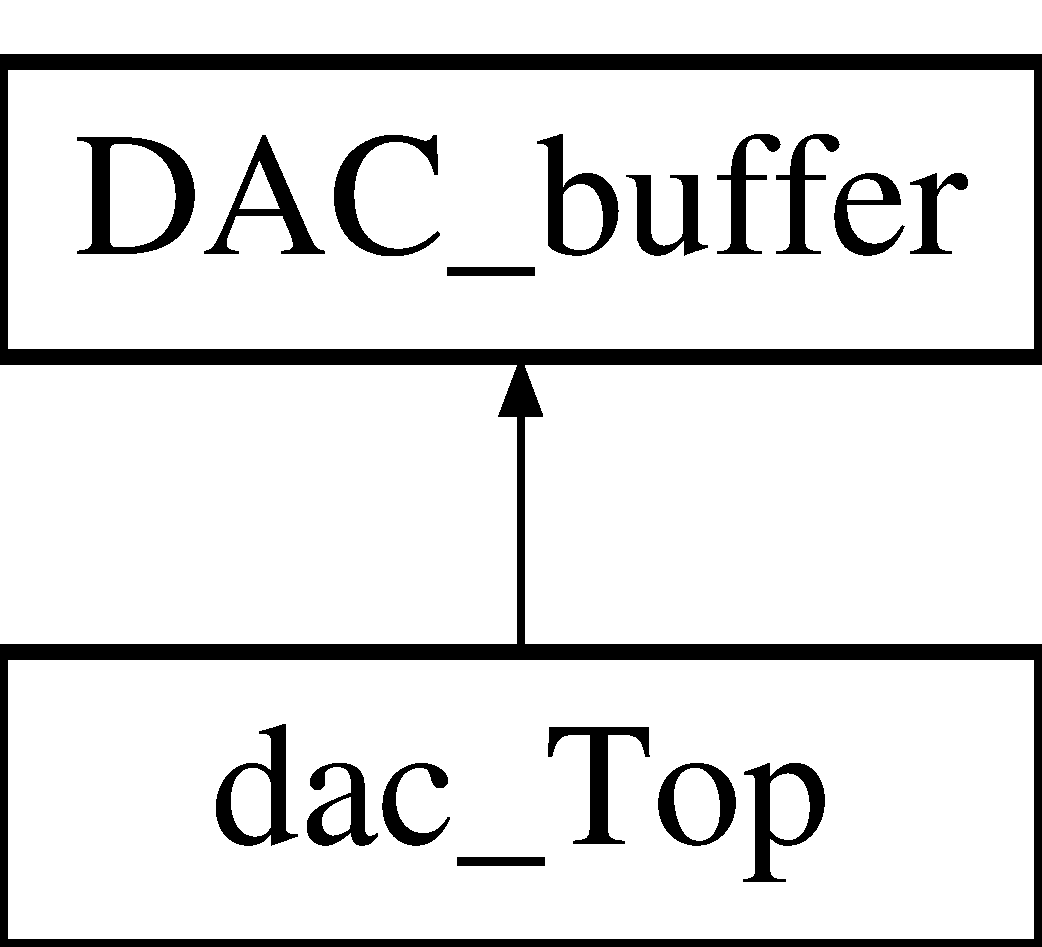
\includegraphics[height=2.000000cm]{classDAC__buffer}
\end{center}
\end{figure}
\subsection*{Entities}
\begin{DoxyCompactItemize}
\item 
\hyperlink{classDAC__buffer_1_1Behavioral}{Behavioral} architecture
\begin{DoxyCompactList}\small\item\em Achitechture of the D\-A\-C buffer. \end{DoxyCompactList}\end{DoxyCompactItemize}
\subsection*{Libraries}
 \begin{DoxyCompactItemize}
\item 
\hypertarget{classDAC__buffer_ae4f03c286607f3181e16b9aa12d0c6d4}{\hyperlink{classDAC__buffer_ae4f03c286607f3181e16b9aa12d0c6d4}{I\-E\-E\-E} }\label{classDAC__buffer_ae4f03c286607f3181e16b9aa12d0c6d4}

\begin{DoxyCompactList}\small\item\em Use of standard library. \end{DoxyCompactList}\end{DoxyCompactItemize}
\subsection*{Use Clauses}
 \begin{DoxyCompactItemize}
\item 
\hypertarget{classDAC__buffer_a68c233289eaf7d2601307bdd93b4c299}{\hyperlink{classDAC__buffer_a68c233289eaf7d2601307bdd93b4c299}{I\-E\-E\-E.\-S\-T\-D\-\_\-\-L\-O\-G\-I\-C\-\_\-1164.\-all}   }\label{classDAC__buffer_a68c233289eaf7d2601307bdd93b4c299}

\begin{DoxyCompactList}\small\item\em Use of standard logic arguments. \end{DoxyCompactList}\item 
\hypertarget{classDAC__buffer_a7c135c43c66ccd7f22abe5f6211788a5}{\hyperlink{classDAC__buffer_a7c135c43c66ccd7f22abe5f6211788a5}{I\-E\-E\-E.\-N\-U\-M\-E\-R\-I\-C\-\_\-\-S\-T\-D.\-all}   }\label{classDAC__buffer_a7c135c43c66ccd7f22abe5f6211788a5}

\begin{DoxyCompactList}\small\item\em Use of standard numerical arguments. \end{DoxyCompactList}\end{DoxyCompactItemize}
\subsection*{Generics}
 \begin{DoxyCompactItemize}
\item 
\hypertarget{classDAC__buffer_a2f94b7b31a8914ee23be5e000f89e921}{\hyperlink{classDAC__buffer_a2f94b7b31a8914ee23be5e000f89e921}{bufferwidth} {\bfseries {\bfseries \textcolor{comment}{integer}\textcolor{vhdlchar}{ }\textcolor{vhdlchar}{\-:}\textcolor{vhdlchar}{=}\textcolor{vhdlchar}{ } \textcolor{vhdldigit}{7} \textcolor{vhdlchar}{ }}}}\label{classDAC__buffer_a2f94b7b31a8914ee23be5e000f89e921}

\begin{DoxyCompactList}\small\item\em Generic indicating the width of the buffer address. \end{DoxyCompactList}\end{DoxyCompactItemize}
\subsection*{Ports}
 \begin{DoxyCompactItemize}
\item 
\hypertarget{classDAC__buffer_a8120037e0ee47c35ba2d79242209c72e}{\hyperlink{classDAC__buffer_a8120037e0ee47c35ba2d79242209c72e}{clk}  {\bfseries {\bfseries \textcolor{vhdlkeyword}{in}\textcolor{vhdlchar}{ }}} {\bfseries \textcolor{comment}{S\-T\-D\-\_\-\-L\-O\-G\-I\-C}\textcolor{vhdlchar}{ }} }\label{classDAC__buffer_a8120037e0ee47c35ba2d79242209c72e}

\begin{DoxyCompactList}\small\item\em Generic indicating the width of the buffer address. \end{DoxyCompactList}\item 
\hypertarget{classDAC__buffer_aa7b7040844189161771c36cf6bbf172c}{\hyperlink{classDAC__buffer_aa7b7040844189161771c36cf6bbf172c}{rst}  {\bfseries {\bfseries \textcolor{vhdlkeyword}{in}\textcolor{vhdlchar}{ }}} {\bfseries \textcolor{comment}{S\-T\-D\-\_\-\-L\-O\-G\-I\-C}\textcolor{vhdlchar}{ }} }\label{classDAC__buffer_aa7b7040844189161771c36cf6bbf172c}

\begin{DoxyCompactList}\small\item\em Global reset, active low. \end{DoxyCompactList}\item 
\hypertarget{classDAC__buffer_a6895d06b697facf19161e9977457e157}{\hyperlink{classDAC__buffer_a6895d06b697facf19161e9977457e157}{buff\-Read}  {\bfseries {\bfseries \textcolor{vhdlkeyword}{in}\textcolor{vhdlchar}{ }}} {\bfseries \textcolor{comment}{S\-T\-D\-\_\-\-L\-O\-G\-I\-C}\textcolor{vhdlchar}{ }} }\label{classDAC__buffer_a6895d06b697facf19161e9977457e157}

\begin{DoxyCompactList}\small\item\em signal to change the read value from the buffer \end{DoxyCompactList}\item 
\hypertarget{classDAC__buffer_a7a77e72065924496dbe7ff565f233c10}{\hyperlink{classDAC__buffer_a7a77e72065924496dbe7ff565f233c10}{index\-Reset}  {\bfseries {\bfseries \textcolor{vhdlkeyword}{in}\textcolor{vhdlchar}{ }}} {\bfseries \textcolor{comment}{S\-T\-D\-\_\-\-L\-O\-G\-I\-C}\textcolor{vhdlchar}{ }} }\label{classDAC__buffer_a7a77e72065924496dbe7ff565f233c10}

\begin{DoxyCompactList}\small\item\em Controls when values are to be stored. \end{DoxyCompactList}\item 
\hypertarget{classDAC__buffer_a51ed8e25642c784ee7d9a51e75716c7c}{\hyperlink{classDAC__buffer_a51ed8e25642c784ee7d9a51e75716c7c}{buff\-Write}  {\bfseries {\bfseries \textcolor{vhdlkeyword}{in}\textcolor{vhdlchar}{ }}} {\bfseries \textcolor{comment}{S\-T\-D\-\_\-\-L\-O\-G\-I\-C}\textcolor{vhdlchar}{ }} }\label{classDAC__buffer_a51ed8e25642c784ee7d9a51e75716c7c}

\begin{DoxyCompactList}\small\item\em controls when to change the output value \end{DoxyCompactList}\item 
\hypertarget{classDAC__buffer_ae70293feb69ea6a383827a243ffce721}{\hyperlink{classDAC__buffer_ae70293feb69ea6a383827a243ffce721}{buff\-In}  {\bfseries {\bfseries \textcolor{vhdlkeyword}{in}\textcolor{vhdlchar}{ }}} {\bfseries \textcolor{comment}{S\-T\-D\-\_\-\-L\-O\-G\-I\-C\-\_\-\-V\-E\-C\-T\-O\-R}\textcolor{vhdlchar}{ }\textcolor{vhdlchar}{(}\textcolor{vhdlchar}{ }\textcolor{vhdlchar}{ } \textcolor{vhdldigit}{15} \textcolor{vhdlchar}{ }\textcolor{vhdlchar}{ }\textcolor{vhdlchar}{ }\textcolor{vhdlkeyword}{downto}\textcolor{vhdlchar}{ }\textcolor{vhdlchar}{ }\textcolor{vhdlchar}{ } \textcolor{vhdldigit}{0} \textcolor{vhdlchar}{ }\textcolor{vhdlchar}{)}\textcolor{vhdlchar}{ }} }\label{classDAC__buffer_ae70293feb69ea6a383827a243ffce721}

\begin{DoxyCompactList}\small\item\em Input value to be stored. \end{DoxyCompactList}\item 
\hypertarget{classDAC__buffer_a7bcaedcfee1dc3d1411311076b527a1a}{\hyperlink{classDAC__buffer_a7bcaedcfee1dc3d1411311076b527a1a}{buff\-Out}  {\bfseries {\bfseries \textcolor{vhdlkeyword}{out}\textcolor{vhdlchar}{ }}} {\bfseries \textcolor{comment}{S\-T\-D\-\_\-\-L\-O\-G\-I\-C\-\_\-\-V\-E\-C\-T\-O\-R}\textcolor{vhdlchar}{ }\textcolor{vhdlchar}{(}\textcolor{vhdlchar}{ }\textcolor{vhdlchar}{ } \textcolor{vhdldigit}{15} \textcolor{vhdlchar}{ }\textcolor{vhdlchar}{ }\textcolor{vhdlchar}{ }\textcolor{vhdlkeyword}{downto}\textcolor{vhdlchar}{ }\textcolor{vhdlchar}{ }\textcolor{vhdlchar}{ } \textcolor{vhdldigit}{0} \textcolor{vhdlchar}{ }\textcolor{vhdlchar}{)}\textcolor{vhdlchar}{ }} }\label{classDAC__buffer_a7bcaedcfee1dc3d1411311076b527a1a}

\begin{DoxyCompactList}\small\item\em Output value from the memory. \end{DoxyCompactList}\item 
\hypertarget{classDAC__buffer_a691d4d7a4daca8bfcaff715e9b7c5dbb}{\hyperlink{classDAC__buffer_a691d4d7a4daca8bfcaff715e9b7c5dbb}{addr}  {\bfseries {\bfseries \textcolor{vhdlkeyword}{in}\textcolor{vhdlchar}{ }}} {\bfseries \textcolor{comment}{S\-T\-D\-\_\-\-L\-O\-G\-I\-C\-\_\-\-V\-E\-C\-T\-O\-R}\textcolor{vhdlchar}{ }\textcolor{vhdlchar}{(}\textcolor{vhdlchar}{ }\textcolor{vhdlchar}{ }{\bfseries \hyperlink{classDAC__buffer_a2f94b7b31a8914ee23be5e000f89e921}{bufferwidth}} \textcolor{vhdlchar}{ }\textcolor{vhdlchar}{-\/}\textcolor{vhdlchar}{ } \textcolor{vhdldigit}{1} \textcolor{vhdlchar}{ }\textcolor{vhdlchar}{ }\textcolor{vhdlchar}{ }\textcolor{vhdlkeyword}{downto}\textcolor{vhdlchar}{ }\textcolor{vhdlchar}{ }\textcolor{vhdlchar}{ } \textcolor{vhdldigit}{0} \textcolor{vhdlchar}{ }\textcolor{vhdlchar}{)}\textcolor{vhdlchar}{ }} }\label{classDAC__buffer_a691d4d7a4daca8bfcaff715e9b7c5dbb}

\begin{DoxyCompactList}\small\item\em Address currently written to. \end{DoxyCompactList}\end{DoxyCompactItemize}


\subsection{Detailed Description}
This component buffers samples from the softcore at the current address when buffwrite is high. The buffer will then output the values on when the buff\-Read goes from low to high. 

The documentation for this class was generated from the following file\-:\begin{DoxyCompactItemize}
\item 
\hyperlink{DAC__BUFFER_8vhd}{D\-A\-C\-\_\-\-B\-U\-F\-F\-E\-R.\-vhd}\end{DoxyCompactItemize}

\hypertarget{classDAC__SPI}{\section{D\-A\-C\-\_\-\-S\-P\-I Entity Reference}
\label{classDAC__SPI}\index{D\-A\-C\-\_\-\-S\-P\-I@{D\-A\-C\-\_\-\-S\-P\-I}}
}


The D\-A\-C \hyperlink{classDAC__SPI_1_1SPI}{S\-P\-I} interface converts parallel data from the data port and transforms it to a \hyperlink{classDAC__SPI_1_1SPI}{S\-P\-I} to be sent to the external D\-A\-C chip on the din port. The module also adds flag bits to this signal, as well as a chip select signal called n\-\_\-sync. The interface listens to the sample clock and only transmits a new message when this clock goes from low to high.  


Inheritance diagram for D\-A\-C\-\_\-\-S\-P\-I\-:\begin{figure}[H]
\begin{center}
\leavevmode
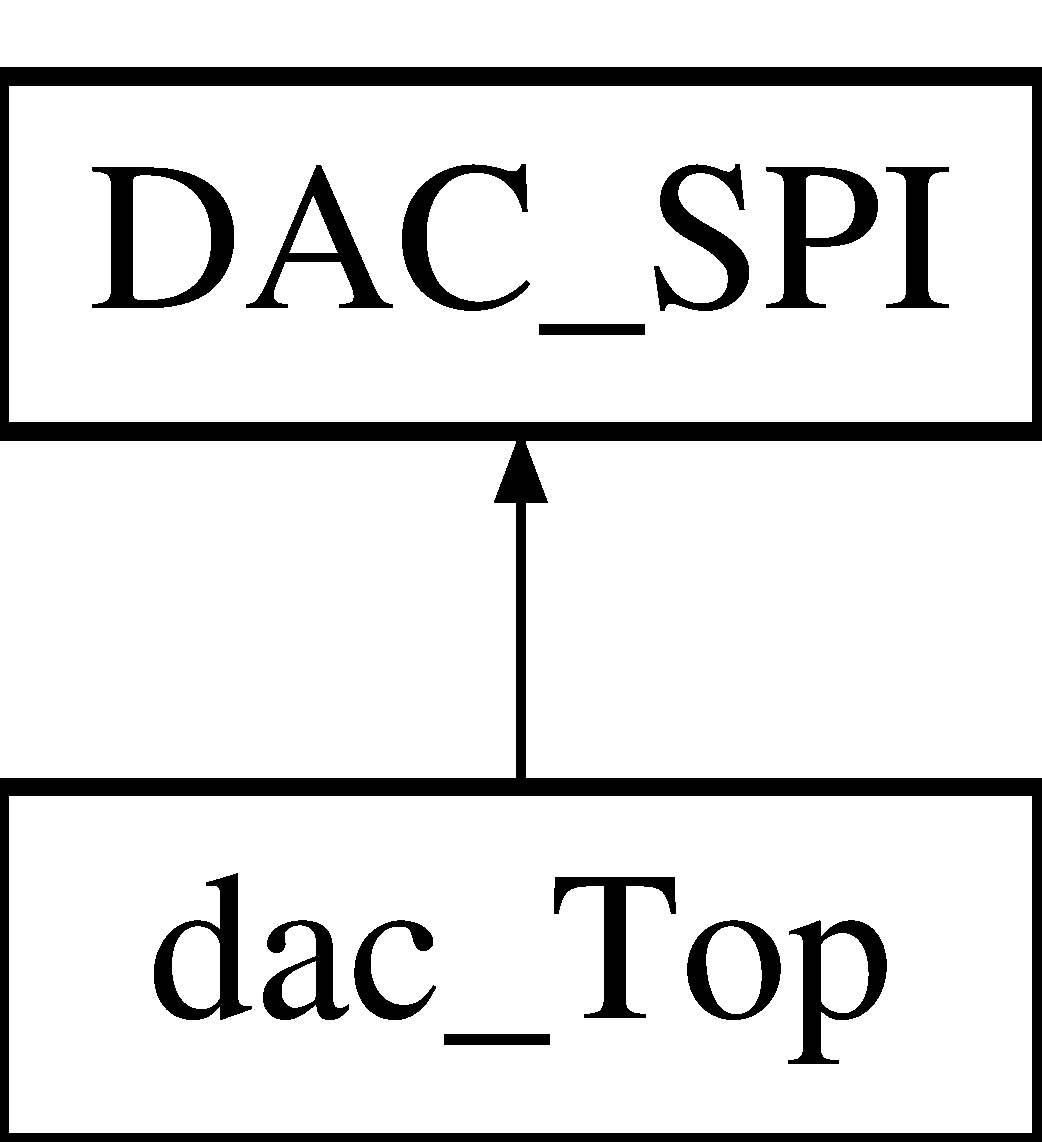
\includegraphics[height=2.000000cm]{classDAC__SPI}
\end{center}
\end{figure}
\subsection*{Entities}
\begin{DoxyCompactItemize}
\item 
\hyperlink{classDAC__SPI_1_1SPI}{S\-P\-I} architecture
\begin{DoxyCompactList}\small\item\em Architecture of the \hyperlink{classDAC__SPI}{D\-A\-C\-\_\-\-S\-P\-I}. \end{DoxyCompactList}\end{DoxyCompactItemize}
\subsection*{Libraries}
 \begin{DoxyCompactItemize}
\item 
\hypertarget{classDAC__SPI_ae4f03c286607f3181e16b9aa12d0c6d4}{\hyperlink{classDAC__SPI_ae4f03c286607f3181e16b9aa12d0c6d4}{I\-E\-E\-E} }\label{classDAC__SPI_ae4f03c286607f3181e16b9aa12d0c6d4}

\begin{DoxyCompactList}\small\item\em Use of standard library. \end{DoxyCompactList}\end{DoxyCompactItemize}
\subsection*{Use Clauses}
 \begin{DoxyCompactItemize}
\item 
\hypertarget{classDAC__SPI_a68c233289eaf7d2601307bdd93b4c299}{\hyperlink{classDAC__SPI_a68c233289eaf7d2601307bdd93b4c299}{I\-E\-E\-E.\-S\-T\-D\-\_\-\-L\-O\-G\-I\-C\-\_\-1164.\-all}   }\label{classDAC__SPI_a68c233289eaf7d2601307bdd93b4c299}

\begin{DoxyCompactList}\small\item\em Use of standard logic arguments. \end{DoxyCompactList}\end{DoxyCompactItemize}
\subsection*{Ports}
 \begin{DoxyCompactItemize}
\item 
\hypertarget{classDAC__SPI_aba021aec4b477b89079bb58ccadcc67e}{\hyperlink{classDAC__SPI_aba021aec4b477b89079bb58ccadcc67e}{rstn}  {\bfseries {\bfseries \textcolor{vhdlkeyword}{in}\textcolor{vhdlchar}{ }}} {\bfseries \textcolor{comment}{S\-T\-D\-\_\-\-L\-O\-G\-I\-C}\textcolor{vhdlchar}{ }} }\label{classDAC__SPI_aba021aec4b477b89079bb58ccadcc67e}

\begin{DoxyCompactList}\small\item\em Global reset active low. \end{DoxyCompactList}\item 
\hypertarget{classDAC__SPI_a8120037e0ee47c35ba2d79242209c72e}{\hyperlink{classDAC__SPI_a8120037e0ee47c35ba2d79242209c72e}{clk}  {\bfseries {\bfseries \textcolor{vhdlkeyword}{in}\textcolor{vhdlchar}{ }}} {\bfseries \textcolor{comment}{S\-T\-D\-\_\-\-L\-O\-G\-I\-C}\textcolor{vhdlchar}{ }} }\label{classDAC__SPI_a8120037e0ee47c35ba2d79242209c72e}

\begin{DoxyCompactList}\small\item\em Clock in, in this case the 25 M\-Hz \hyperlink{classDAC__SPI_1_1SPI}{S\-P\-I} clock. \end{DoxyCompactList}\item 
\hypertarget{classDAC__SPI_a2cc65ad6f0f6d24cd3ebac8757953224}{\hyperlink{classDAC__SPI_a2cc65ad6f0f6d24cd3ebac8757953224}{data}  {\bfseries {\bfseries \textcolor{vhdlkeyword}{in}\textcolor{vhdlchar}{ }}} {\bfseries \textcolor{comment}{S\-T\-D\-\_\-\-L\-O\-G\-I\-C\-\_\-\-V\-E\-C\-T\-O\-R}\textcolor{vhdlchar}{ }\textcolor{vhdlchar}{(}\textcolor{vhdlchar}{ }\textcolor{vhdlchar}{ } \textcolor{vhdldigit}{15} \textcolor{vhdlchar}{ }\textcolor{vhdlchar}{ }\textcolor{vhdlchar}{ }\textcolor{vhdlkeyword}{downto}\textcolor{vhdlchar}{ }\textcolor{vhdlchar}{ }\textcolor{vhdlchar}{ } \textcolor{vhdldigit}{0} \textcolor{vhdlchar}{ }\textcolor{vhdlchar}{)}\textcolor{vhdlchar}{ }} }\label{classDAC__SPI_a2cc65ad6f0f6d24cd3ebac8757953224}

\begin{DoxyCompactList}\small\item\em Data vector containing the parallel sample. \end{DoxyCompactList}\item 
\hypertarget{classDAC__SPI_a4696bc4e06c727fae1b8ce3ba8cf08d4}{\hyperlink{classDAC__SPI_a4696bc4e06c727fae1b8ce3ba8cf08d4}{sampleclk}  {\bfseries {\bfseries \textcolor{vhdlkeyword}{in}\textcolor{vhdlchar}{ }}} {\bfseries \textcolor{comment}{S\-T\-D\-\_\-\-L\-O\-G\-I\-C}\textcolor{vhdlchar}{ }} }\label{classDAC__SPI_a4696bc4e06c727fae1b8ce3ba8cf08d4}

\begin{DoxyCompactList}\small\item\em The sampleclock indicating a new sample is available, this triggers a new transmission. \end{DoxyCompactList}\item 
\hypertarget{classDAC__SPI_a85ffcdebe13d1f5ddc75d9dc2718accd}{\hyperlink{classDAC__SPI_a85ffcdebe13d1f5ddc75d9dc2718accd}{din}  {\bfseries {\bfseries \textcolor{vhdlkeyword}{out}\textcolor{vhdlchar}{ }}} {\bfseries \textcolor{comment}{std\-\_\-logic}\textcolor{vhdlchar}{ }} }\label{classDAC__SPI_a85ffcdebe13d1f5ddc75d9dc2718accd}

\begin{DoxyCompactList}\small\item\em din is the serial connected to the D\-A\-C I\-C \end{DoxyCompactList}\item 
\hypertarget{classDAC__SPI_acb508fc1279abe4c1bc2be47e4dd526b}{\hyperlink{classDAC__SPI_acb508fc1279abe4c1bc2be47e4dd526b}{n\-Sync}  {\bfseries {\bfseries \textcolor{vhdlkeyword}{out}\textcolor{vhdlchar}{ }}} {\bfseries \textcolor{comment}{S\-T\-D\-\_\-\-L\-O\-G\-I\-C}\textcolor{vhdlchar}{ }} }\label{classDAC__SPI_acb508fc1279abe4c1bc2be47e4dd526b}

\begin{DoxyCompactList}\small\item\em nsync is the chip select for the D\-A\-C I\-C \end{DoxyCompactList}\end{DoxyCompactItemize}


\subsection{Detailed Description}
The D\-A\-C \hyperlink{classDAC__SPI_1_1SPI}{S\-P\-I} interface converts parallel data from the data port and transforms it to a \hyperlink{classDAC__SPI_1_1SPI}{S\-P\-I} to be sent to the external D\-A\-C chip on the din port. The module also adds flag bits to this signal, as well as a chip select signal called n\-\_\-sync. The interface listens to the sample clock and only transmits a new message when this clock goes from low to high. 

The documentation for this class was generated from the following file\-:\begin{DoxyCompactItemize}
\item 
\hyperlink{DAC__SPI_8vhd}{D\-A\-C\-\_\-\-S\-P\-I.\-vhd}\end{DoxyCompactItemize}

\hypertarget{classdac__Top}{\section{dac\-\_\-\-Top Entity Reference}
\label{classdac__Top}\index{dac\-\_\-\-Top@{dac\-\_\-\-Top}}
}


This component is a wrapper for the parts needed for the digital to analog converter. Its main functionality is to provide for internal connections between the components and to throughput any signals to the next level in the hierarchy.  


Inheritance diagram for dac\-\_\-\-Top\-:\begin{figure}[H]
\begin{center}
\leavevmode
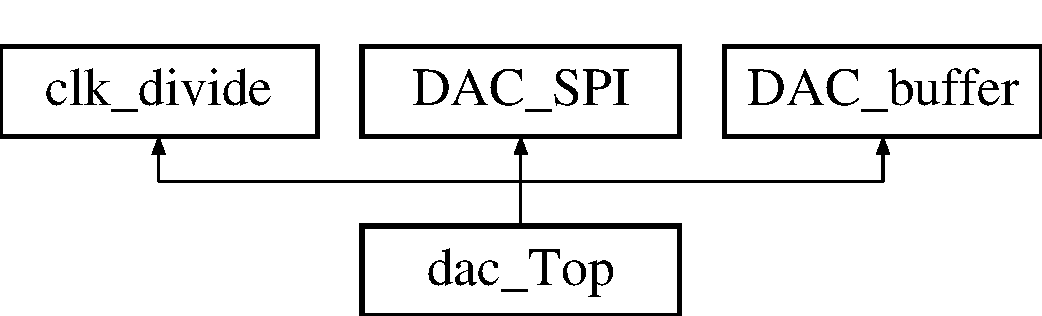
\includegraphics[height=2.000000cm]{classdac__Top}
\end{center}
\end{figure}
\subsection*{Entities}
\begin{DoxyCompactItemize}
\item 
\hyperlink{classdac__Top_1_1TOP__DAC}{T\-O\-P\-\_\-\-D\-A\-C} architecture
\begin{DoxyCompactList}\small\item\em Architecture of the D\-A\-C\-T\-O\-P. \end{DoxyCompactList}\end{DoxyCompactItemize}
\subsection*{Libraries}
 \begin{DoxyCompactItemize}
\item 
\hypertarget{classdac__Top_ae4f03c286607f3181e16b9aa12d0c6d4}{\hyperlink{classdac__Top_ae4f03c286607f3181e16b9aa12d0c6d4}{I\-E\-E\-E} }\label{classdac__Top_ae4f03c286607f3181e16b9aa12d0c6d4}

\begin{DoxyCompactList}\small\item\em Use of standard library. \end{DoxyCompactList}\end{DoxyCompactItemize}
\subsection*{Use Clauses}
 \begin{DoxyCompactItemize}
\item 
\hypertarget{classdac__Top_a68c233289eaf7d2601307bdd93b4c299}{\hyperlink{classdac__Top_a68c233289eaf7d2601307bdd93b4c299}{I\-E\-E\-E.\-S\-T\-D\-\_\-\-L\-O\-G\-I\-C\-\_\-1164.\-all}   }\label{classdac__Top_a68c233289eaf7d2601307bdd93b4c299}

\begin{DoxyCompactList}\small\item\em Use of standard logic arguments. \end{DoxyCompactList}\end{DoxyCompactItemize}
\subsection*{Ports}
 \begin{DoxyCompactItemize}
\item 
\hypertarget{classdac__Top_aba021aec4b477b89079bb58ccadcc67e}{\hyperlink{classdac__Top_aba021aec4b477b89079bb58ccadcc67e}{rstn}  {\bfseries {\bfseries \textcolor{vhdlkeyword}{in}\textcolor{vhdlchar}{ }}} {\bfseries \textcolor{comment}{S\-T\-D\-\_\-\-L\-O\-G\-I\-C}\textcolor{vhdlchar}{ }} }\label{classdac__Top_aba021aec4b477b89079bb58ccadcc67e}

\begin{DoxyCompactList}\small\item\em Global reset, active low. \end{DoxyCompactList}\item 
\hypertarget{classdac__Top_a8120037e0ee47c35ba2d79242209c72e}{\hyperlink{classdac__Top_a8120037e0ee47c35ba2d79242209c72e}{clk}  {\bfseries {\bfseries \textcolor{vhdlkeyword}{in}\textcolor{vhdlchar}{ }}} {\bfseries \textcolor{comment}{S\-T\-D\-\_\-\-L\-O\-G\-I\-C}\textcolor{vhdlchar}{ }} }\label{classdac__Top_a8120037e0ee47c35ba2d79242209c72e}

\begin{DoxyCompactList}\small\item\em Global clock running on 100 M\-Hz to provide maximum accuracy for the sampling clock. \end{DoxyCompactList}\item 
\hypertarget{classdac__Top_a4f305185694168405a38c701331c178e}{\hyperlink{classdac__Top_a4f305185694168405a38c701331c178e}{clk50\-M\-Hz}  {\bfseries {\bfseries \textcolor{vhdlkeyword}{in}\textcolor{vhdlchar}{ }}} {\bfseries \textcolor{comment}{S\-T\-D\-\_\-\-L\-O\-G\-I\-C}\textcolor{vhdlchar}{ }} }\label{classdac__Top_a4f305185694168405a38c701331c178e}

\begin{DoxyCompactList}\small\item\em Global L\-E\-O\-N clock running at 50 M\-Hz for everything else. \end{DoxyCompactList}\item 
\hypertarget{classdac__Top_a2cc65ad6f0f6d24cd3ebac8757953224}{\hyperlink{classdac__Top_a2cc65ad6f0f6d24cd3ebac8757953224}{data}  {\bfseries {\bfseries \textcolor{vhdlkeyword}{in}\textcolor{vhdlchar}{ }}} {\bfseries \textcolor{comment}{S\-T\-D\-\_\-\-L\-O\-G\-I\-C\-\_\-\-V\-E\-C\-T\-O\-R}\textcolor{vhdlchar}{ }\textcolor{vhdlchar}{(}\textcolor{vhdlchar}{ }\textcolor{vhdlchar}{ } \textcolor{vhdldigit}{15} \textcolor{vhdlchar}{ }\textcolor{vhdlchar}{ }\textcolor{vhdlchar}{ }\textcolor{vhdlkeyword}{downto}\textcolor{vhdlchar}{ }\textcolor{vhdlchar}{ }\textcolor{vhdlchar}{ } \textcolor{vhdldigit}{0} \textcolor{vhdlchar}{ }\textcolor{vhdlchar}{)}\textcolor{vhdlchar}{ }} }\label{classdac__Top_a2cc65ad6f0f6d24cd3ebac8757953224}

\begin{DoxyCompactList}\small\item\em Data in from the softcore output. \end{DoxyCompactList}\item 
\hypertarget{classdac__Top_ad1620b7fc57dbb860b23d27c24034285}{\hyperlink{classdac__Top_ad1620b7fc57dbb860b23d27c24034285}{addr}  {\bfseries {\bfseries \textcolor{vhdlkeyword}{in}\textcolor{vhdlchar}{ }}} {\bfseries \textcolor{comment}{S\-T\-D\-\_\-\-L\-O\-G\-I\-C\-\_\-\-V\-E\-C\-T\-O\-R}\textcolor{vhdlchar}{ }\textcolor{vhdlchar}{(}\textcolor{vhdlchar}{ }\textcolor{vhdlchar}{ } \textcolor{vhdldigit}{6} \textcolor{vhdlchar}{ }\textcolor{vhdlchar}{ }\textcolor{vhdlchar}{ }\textcolor{vhdlkeyword}{downto}\textcolor{vhdlchar}{ }\textcolor{vhdlchar}{ }\textcolor{vhdlchar}{ } \textcolor{vhdldigit}{0} \textcolor{vhdlchar}{ }\textcolor{vhdlchar}{)}\textcolor{vhdlchar}{ }} }\label{classdac__Top_ad1620b7fc57dbb860b23d27c24034285}

\begin{DoxyCompactList}\small\item\em Address from the softcore. \end{DoxyCompactList}\item 
\hypertarget{classdac__Top_a042a830e6d62a56ff50a9a3e85ff86dd}{\hyperlink{classdac__Top_a042a830e6d62a56ff50a9a3e85ff86dd}{write}  {\bfseries {\bfseries \textcolor{vhdlkeyword}{in}\textcolor{vhdlchar}{ }}} {\bfseries \textcolor{comment}{S\-T\-D\-\_\-\-L\-O\-G\-I\-C}\textcolor{vhdlchar}{ }} }\label{classdac__Top_a042a830e6d62a56ff50a9a3e85ff86dd}

\begin{DoxyCompactList}\small\item\em Signal indicating the buffers to read values. \end{DoxyCompactList}\item 
\hypertarget{classdac__Top_aae112fd9041e6fcce9483ea8550d54f3}{\hyperlink{classdac__Top_aae112fd9041e6fcce9483ea8550d54f3}{sampleclk}  {\bfseries {\bfseries \textcolor{vhdlkeyword}{out}\textcolor{vhdlchar}{ }}} {\bfseries \textcolor{comment}{S\-T\-D\-\_\-\-L\-O\-G\-I\-C}\textcolor{vhdlchar}{ }} }\label{classdac__Top_aae112fd9041e6fcce9483ea8550d54f3}

\begin{DoxyCompactList}\small\item\em The sampleclock running at 705.\-6 k\-Hz, used by A\-D\-C for oversampling. \end{DoxyCompactList}\item 
\hypertarget{classdac__Top_a70a8575229cff595728858aea9bd6a65}{\hyperlink{classdac__Top_a70a8575229cff595728858aea9bd6a65}{sampleclk44khz}  {\bfseries {\bfseries \textcolor{vhdlkeyword}{out}\textcolor{vhdlchar}{ }}} {\bfseries \textcolor{comment}{S\-T\-D\-\_\-\-L\-O\-G\-I\-C}\textcolor{vhdlchar}{ }} }\label{classdac__Top_a70a8575229cff595728858aea9bd6a65}

\begin{DoxyCompactList}\small\item\em A sampleclock indicating a new sample were to be read to/from buffers. \end{DoxyCompactList}\item 
\hypertarget{classdac__Top_a6d01fe70bfcd66f305c9c962331782cd}{\hyperlink{classdac__Top_a6d01fe70bfcd66f305c9c962331782cd}{sclk}  {\bfseries {\bfseries \textcolor{vhdlkeyword}{out}\textcolor{vhdlchar}{ }}} {\bfseries \textcolor{comment}{S\-T\-D\-\_\-\-L\-O\-G\-I\-C}\textcolor{vhdlchar}{ }} }\label{classdac__Top_a6d01fe70bfcd66f305c9c962331782cd}

\begin{DoxyCompactList}\small\item\em A clock for the off chip D\-A\-C chip. \end{DoxyCompactList}\item 
\hypertarget{classdac__Top_a85ffcdebe13d1f5ddc75d9dc2718accd}{\hyperlink{classdac__Top_a85ffcdebe13d1f5ddc75d9dc2718accd}{din}  {\bfseries {\bfseries \textcolor{vhdlkeyword}{out}\textcolor{vhdlchar}{ }}} {\bfseries \textcolor{comment}{std\-\_\-logic}\textcolor{vhdlchar}{ }} }\label{classdac__Top_a85ffcdebe13d1f5ddc75d9dc2718accd}

\begin{DoxyCompactList}\small\item\em The output sample in serial to the off chip D\-A\-C. \end{DoxyCompactList}\item 
\hypertarget{classdac__Top_acb508fc1279abe4c1bc2be47e4dd526b}{\hyperlink{classdac__Top_acb508fc1279abe4c1bc2be47e4dd526b}{n\-Sync}  {\bfseries {\bfseries \textcolor{vhdlkeyword}{out}\textcolor{vhdlchar}{ }}} {\bfseries \textcolor{comment}{S\-T\-D\-\_\-\-L\-O\-G\-I\-C}\textcolor{vhdlchar}{ }} }\label{classdac__Top_acb508fc1279abe4c1bc2be47e4dd526b}

\begin{DoxyCompactList}\small\item\em The output sync to the off chip D\-A\-C. \end{DoxyCompactList}\item 
\hypertarget{classdac__Top_a5a1c2c67d9bb87333434aa5bbc7217ac}{\hyperlink{classdac__Top_a5a1c2c67d9bb87333434aa5bbc7217ac}{index\-\_\-reset}  {\bfseries {\bfseries \textcolor{vhdlkeyword}{in}\textcolor{vhdlchar}{ }}} {\bfseries \textcolor{comment}{S\-T\-D\-\_\-logic}\textcolor{vhdlchar}{ }} }\label{classdac__Top_a5a1c2c67d9bb87333434aa5bbc7217ac}

\begin{DoxyCompactList}\small\item\em A signal to reset the memory counter. \end{DoxyCompactList}\end{DoxyCompactItemize}


\subsection{Detailed Description}
This component is a wrapper for the parts needed for the digital to analog converter. Its main functionality is to provide for internal connections between the components and to throughput any signals to the next level in the hierarchy. 

The documentation for this class was generated from the following file\-:\begin{DoxyCompactItemize}
\item 
\hyperlink{DAC__TOP_8vhd}{D\-A\-C\-\_\-\-T\-O\-P.\-vhd}\end{DoxyCompactItemize}

\hypertarget{classdigitalfilter}{\section{digitalfilter Entity Reference}
\label{classdigitalfilter}\index{digitalfilter@{digitalfilter}}
}


This module implements a digital F\-I\-R filter. When the start port goes from low to high the filter will shift a storage vector and sample the current input value. The filter than multiplies and accumulates once evety clock cycle until the calculations are done. When this happenes the calculated value is outputted and the finished port will be set.  


Inheritance diagram for digitalfilter\-:\begin{figure}[H]
\begin{center}
\leavevmode
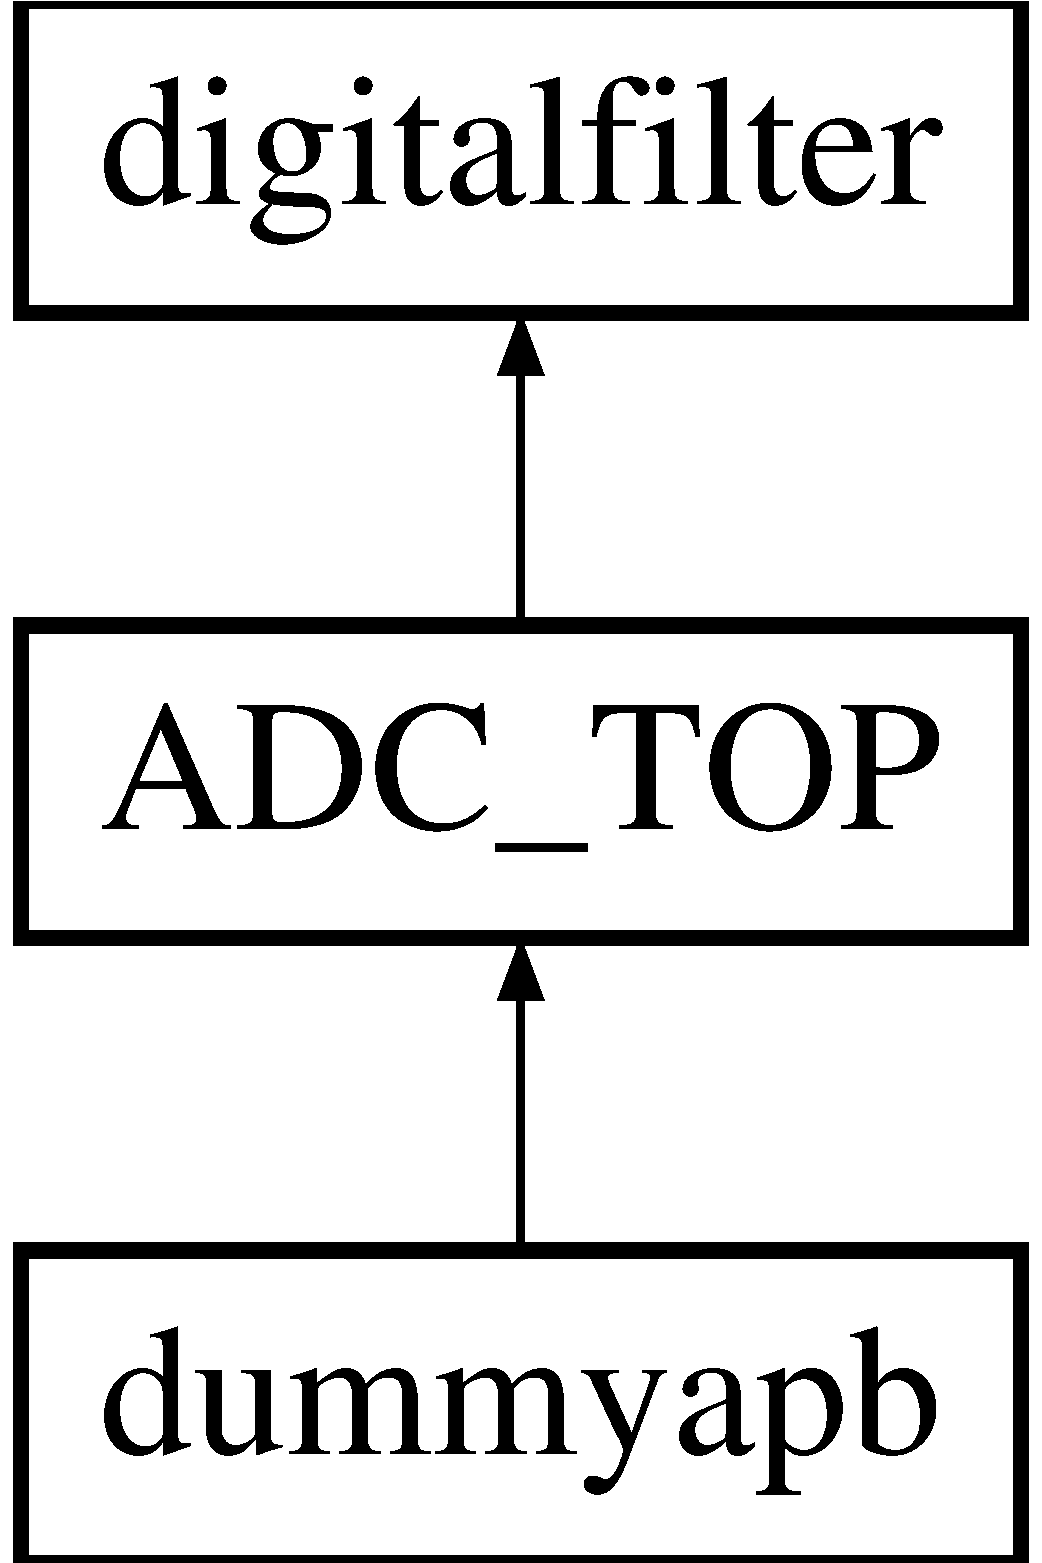
\includegraphics[height=2.000000cm]{classdigitalfilter}
\end{center}
\end{figure}
\subsection*{Entities}
\begin{DoxyCompactItemize}
\item 
\hyperlink{classdigitalfilter_1_1Behavioral}{Behavioral} architecture
\begin{DoxyCompactList}\small\item\em Architecture of the digitalfilter. \end{DoxyCompactList}\end{DoxyCompactItemize}
\subsection*{Libraries}
 \begin{DoxyCompactItemize}
\item 
\hypertarget{classdigitalfilter_ae4f03c286607f3181e16b9aa12d0c6d4}{\hyperlink{classdigitalfilter_ae4f03c286607f3181e16b9aa12d0c6d4}{I\-E\-E\-E} }\label{classdigitalfilter_ae4f03c286607f3181e16b9aa12d0c6d4}

\begin{DoxyCompactList}\small\item\em Use of standard library. \end{DoxyCompactList}\end{DoxyCompactItemize}
\subsection*{Use Clauses}
 \begin{DoxyCompactItemize}
\item 
\hypertarget{classdigitalfilter_a68c233289eaf7d2601307bdd93b4c299}{\hyperlink{classdigitalfilter_a68c233289eaf7d2601307bdd93b4c299}{I\-E\-E\-E.\-S\-T\-D\-\_\-\-L\-O\-G\-I\-C\-\_\-1164.\-all}   }\label{classdigitalfilter_a68c233289eaf7d2601307bdd93b4c299}

\begin{DoxyCompactList}\small\item\em Use of standard logic arguments. \end{DoxyCompactList}\item 
\hypertarget{classdigitalfilter_a7c135c43c66ccd7f22abe5f6211788a5}{\hyperlink{classdigitalfilter_a7c135c43c66ccd7f22abe5f6211788a5}{I\-E\-E\-E.\-N\-U\-M\-E\-R\-I\-C\-\_\-\-S\-T\-D.\-all}   }\label{classdigitalfilter_a7c135c43c66ccd7f22abe5f6211788a5}

\begin{DoxyCompactList}\small\item\em Use of standard numerical arguments. \end{DoxyCompactList}\end{DoxyCompactItemize}
\subsection*{Generics}
 \begin{DoxyCompactItemize}
\item 
\hypertarget{classdigitalfilter_a91fcbc2cb8dd91f914c30526e23794a9}{\hyperlink{classdigitalfilter_a91fcbc2cb8dd91f914c30526e23794a9}{W\-I\-D\-T\-H} {\bfseries {\bfseries \textcolor{comment}{I\-N\-T\-E\-G\-E\-R}\textcolor{vhdlchar}{ }\textcolor{vhdlchar}{\-:}\textcolor{vhdlchar}{=}\textcolor{vhdlchar}{ } \textcolor{vhdldigit}{8} \textcolor{vhdlchar}{ }}}}\label{classdigitalfilter_a91fcbc2cb8dd91f914c30526e23794a9}

\begin{DoxyCompactList}\small\item\em Width decides the bitwidth of the filter. \end{DoxyCompactList}\item 
\hypertarget{classdigitalfilter_a61de7093f96d3bc9f246d1d7744f9dc6}{\hyperlink{classdigitalfilter_a61de7093f96d3bc9f246d1d7744f9dc6}{N} {\bfseries {\bfseries \textcolor{comment}{I\-N\-T\-E\-G\-E\-R}\textcolor{vhdlchar}{ }\textcolor{vhdlchar}{\-:}\textcolor{vhdlchar}{=}\textcolor{vhdlchar}{ } \textcolor{vhdldigit}{4} \textcolor{vhdlchar}{ }}}}\label{classdigitalfilter_a61de7093f96d3bc9f246d1d7744f9dc6}

\begin{DoxyCompactList}\small\item\em N descides the number of taps of the filter. \end{DoxyCompactList}\end{DoxyCompactItemize}
\subsection*{Ports}
 \begin{DoxyCompactItemize}
\item 
\hypertarget{classdigitalfilter_aae5de5c5aebf7b54ecd36feaba217215}{\hyperlink{classdigitalfilter_aae5de5c5aebf7b54ecd36feaba217215}{reset}  {\bfseries {\bfseries \textcolor{vhdlkeyword}{in}\textcolor{vhdlchar}{ }}} {\bfseries \textcolor{comment}{S\-T\-D\-\_\-\-L\-O\-G\-I\-C}\textcolor{vhdlchar}{ }} }\label{classdigitalfilter_aae5de5c5aebf7b54ecd36feaba217215}

\begin{DoxyCompactList}\small\item\em reset, active low \end{DoxyCompactList}\item 
\hypertarget{classdigitalfilter_a4c6f5b721113d4ad96eb10f383e44e7a}{\hyperlink{classdigitalfilter_a4c6f5b721113d4ad96eb10f383e44e7a}{start}  {\bfseries {\bfseries \textcolor{vhdlkeyword}{in}\textcolor{vhdlchar}{ }}} {\bfseries \textcolor{comment}{S\-T\-D\-\_\-\-L\-O\-G\-I\-C}\textcolor{vhdlchar}{ }} }\label{classdigitalfilter_a4c6f5b721113d4ad96eb10f383e44e7a}

\begin{DoxyCompactList}\small\item\em start indicates a new value is available, starting the calculations in the filter \end{DoxyCompactList}\item 
\hypertarget{classdigitalfilter_a8120037e0ee47c35ba2d79242209c72e}{\hyperlink{classdigitalfilter_a8120037e0ee47c35ba2d79242209c72e}{clk}  {\bfseries {\bfseries \textcolor{vhdlkeyword}{in}\textcolor{vhdlchar}{ }}} {\bfseries \textcolor{comment}{S\-T\-D\-\_\-\-L\-O\-G\-I\-C}\textcolor{vhdlchar}{ }} }\label{classdigitalfilter_a8120037e0ee47c35ba2d79242209c72e}

\begin{DoxyCompactList}\small\item\em clock for the filter operations \end{DoxyCompactList}\item 
\hypertarget{classdigitalfilter_a8c5602ac7769fa0806595aa864d2134b}{\hyperlink{classdigitalfilter_a8c5602ac7769fa0806595aa864d2134b}{x}  {\bfseries {\bfseries \textcolor{vhdlkeyword}{in}\textcolor{vhdlchar}{ }}} {\bfseries \textcolor{comment}{S\-T\-D\-\_\-\-L\-O\-G\-I\-C\-\_\-\-V\-E\-C\-T\-O\-R}\textcolor{vhdlchar}{ }\textcolor{vhdlchar}{(}\textcolor{vhdlchar}{ }\textcolor{vhdlchar}{ }{\bfseries \hyperlink{classdigitalfilter_a91fcbc2cb8dd91f914c30526e23794a9}{W\-I\-D\-T\-H}} \textcolor{vhdlchar}{ }\textcolor{vhdlchar}{-\/}\textcolor{vhdlchar}{ } \textcolor{vhdldigit}{1} \textcolor{vhdlchar}{ }\textcolor{vhdlchar}{ }\textcolor{vhdlchar}{ }\textcolor{vhdlkeyword}{downto}\textcolor{vhdlchar}{ }\textcolor{vhdlchar}{ }\textcolor{vhdlchar}{ } \textcolor{vhdldigit}{0} \textcolor{vhdlchar}{ }\textcolor{vhdlchar}{)}\textcolor{vhdlchar}{ }} }\label{classdigitalfilter_a8c5602ac7769fa0806595aa864d2134b}

\begin{DoxyCompactList}\small\item\em x is the input of the filter \end{DoxyCompactList}\item 
\hypertarget{classdigitalfilter_af668726c6bb16ef4d276739c4c161217}{\hyperlink{classdigitalfilter_af668726c6bb16ef4d276739c4c161217}{y}  {\bfseries {\bfseries \textcolor{vhdlkeyword}{out}\textcolor{vhdlchar}{ }}} {\bfseries \textcolor{comment}{S\-T\-D\-\_\-\-L\-O\-G\-I\-C\-\_\-\-V\-E\-C\-T\-O\-R}\textcolor{vhdlchar}{ }\textcolor{vhdlchar}{(}\textcolor{vhdlchar}{ }\textcolor{vhdlchar}{ } \textcolor{vhdldigit}{31} \textcolor{vhdlchar}{ }\textcolor{vhdlchar}{ }\textcolor{vhdlchar}{ }\textcolor{vhdlkeyword}{downto}\textcolor{vhdlchar}{ }\textcolor{vhdlchar}{ }\textcolor{vhdlchar}{ } \textcolor{vhdldigit}{0} \textcolor{vhdlchar}{ }\textcolor{vhdlchar}{)}\textcolor{vhdlchar}{ }} }\label{classdigitalfilter_af668726c6bb16ef4d276739c4c161217}

\begin{DoxyCompactList}\small\item\em y is the outpu of the filter \end{DoxyCompactList}\item 
\hypertarget{classdigitalfilter_ad2b5eab2bb63ad6b267ff2523ac34898}{\hyperlink{classdigitalfilter_ad2b5eab2bb63ad6b267ff2523ac34898}{finished}  {\bfseries {\bfseries \textcolor{vhdlkeyword}{out}\textcolor{vhdlchar}{ }}} {\bfseries \textcolor{comment}{S\-T\-D\-\_\-\-L\-O\-G\-I\-C}\textcolor{vhdlchar}{ }} }\label{classdigitalfilter_ad2b5eab2bb63ad6b267ff2523ac34898}

\begin{DoxyCompactList}\small\item\em finished indicates the filter calculations are done \end{DoxyCompactList}\end{DoxyCompactItemize}


\subsection{Detailed Description}
This module implements a digital F\-I\-R filter. When the start port goes from low to high the filter will shift a storage vector and sample the current input value. The filter than multiplies and accumulates once evety clock cycle until the calculations are done. When this happenes the calculated value is outputted and the finished port will be set. 

The documentation for this class was generated from the following file\-:\begin{DoxyCompactItemize}
\item 
\hyperlink{digitalfilter_8vhd}{digitalfilter.\-vhd}\end{DoxyCompactItemize}

\hypertarget{classRGB__diode__controller_1_1diode}{\section{diode Architecture Reference}
\label{classRGB__diode__controller_1_1diode}\index{diode@{diode}}
}


Architecture of the R\-G\-B\-\_\-diode.  


\subsection*{Processes}
 \begin{DoxyCompactItemize}
\item 
\hypertarget{classRGB__diode__controller_1_1diode_a9e039d1336ed36e47c247368cdc9b80b}{\hyperlink{classRGB__diode__controller_1_1diode_a9e039d1336ed36e47c247368cdc9b80b}{P\-R\-O\-C\-E\-S\-S\-\_\-8}{\bfseries  ( {\bfseries {\bfseries \hyperlink{classRGB__diode__controller_aba021aec4b477b89079bb58ccadcc67e}{rstn}} \textcolor{vhdlchar}{ }\textcolor{vhdlchar}{ }\textcolor{vhdlchar}{ }} , {\bfseries {\bfseries \hyperlink{classRGB__diode__controller_a8120037e0ee47c35ba2d79242209c72e}{clk}} \textcolor{vhdlchar}{ }} )}}\label{classRGB__diode__controller_1_1diode_a9e039d1336ed36e47c247368cdc9b80b}

\end{DoxyCompactItemize}
\subsection*{Signals}
 \begin{DoxyCompactItemize}
\item 
\hypertarget{classRGB__diode__controller_1_1diode_a36d6c358f271c34f9fba99138b3bddf2}{\hyperlink{classRGB__diode__controller_1_1diode_a36d6c358f271c34f9fba99138b3bddf2}{diode\-\_\-duty\-\_\-counter} {\bfseries \textcolor{comment}{integer}\textcolor{vhdlchar}{ }\textcolor{vhdlkeyword}{range}\textcolor{vhdlchar}{ } \textcolor{vhdldigit}{0} \textcolor{vhdlchar}{ }\textcolor{vhdlchar}{ }\textcolor{vhdlchar}{ }\textcolor{vhdlkeyword}{to}\textcolor{vhdlchar}{ }\textcolor{vhdlchar}{ }\textcolor{vhdlchar}{ }{\bfseries \hyperlink{classRGB__diode__controller_ad3971b999c08c97da803416025fcebb0}{N}} \textcolor{vhdlchar}{ }} }\label{classRGB__diode__controller_1_1diode_a36d6c358f271c34f9fba99138b3bddf2}

\begin{DoxyCompactList}\small\item\em A counter for the duty cycle. \end{DoxyCompactList}\item 
\hypertarget{classRGB__diode__controller_1_1diode_a471ca34f0f3e1757f74b6c21eb6c97ed}{\hyperlink{classRGB__diode__controller_1_1diode_a471ca34f0f3e1757f74b6c21eb6c97ed}{diode\-\_\-enable} {\bfseries \textcolor{comment}{S\-T\-D\-\_\-\-L\-O\-G\-I\-C\-\_\-vector}\textcolor{vhdlchar}{ }\textcolor{vhdlchar}{(}\textcolor{vhdlchar}{ }\textcolor{vhdlchar}{ } \textcolor{vhdldigit}{2} \textcolor{vhdlchar}{ }\textcolor{vhdlchar}{ }\textcolor{vhdlchar}{ }\textcolor{vhdlkeyword}{downto}\textcolor{vhdlchar}{ }\textcolor{vhdlchar}{ }\textcolor{vhdlchar}{ } \textcolor{vhdldigit}{0} \textcolor{vhdlchar}{ }\textcolor{vhdlchar}{)}\textcolor{vhdlchar}{ }} }\label{classRGB__diode__controller_1_1diode_a471ca34f0f3e1757f74b6c21eb6c97ed}

\begin{DoxyCompactList}\small\item\em A enable to indicate if a diode should be lit. \end{DoxyCompactList}\end{DoxyCompactItemize}


\subsection{Detailed Description}
Architecture of the R\-G\-B\-\_\-diode. 

The R\-G\-B\-\_\-control changed the R\-G\-B diodes color depending on the state of the input is\-\_\-working. Depending of the generic N the brightness of the diode can also be controlled as an N of 0 proved to bright 

The documentation for this class was generated from the following file\-:\begin{DoxyCompactItemize}
\item 
\hyperlink{RGB__diode__controller_8vhd}{R\-G\-B\-\_\-diode\-\_\-controller.\-vhd}\end{DoxyCompactItemize}

\hypertarget{classdummyapb}{\section{dummyapb Entity Reference}
\label{classdummyapb}\index{dummyapb@{dummyapb}}
}


This component gathers all the sub-\/modules needed for communication with A\-D\-C and D\-A\-C. It also supplies an interface to the A\-P\-B bus.  


Inheritance diagram for dummyapb\-:\begin{figure}[H]
\begin{center}
\leavevmode
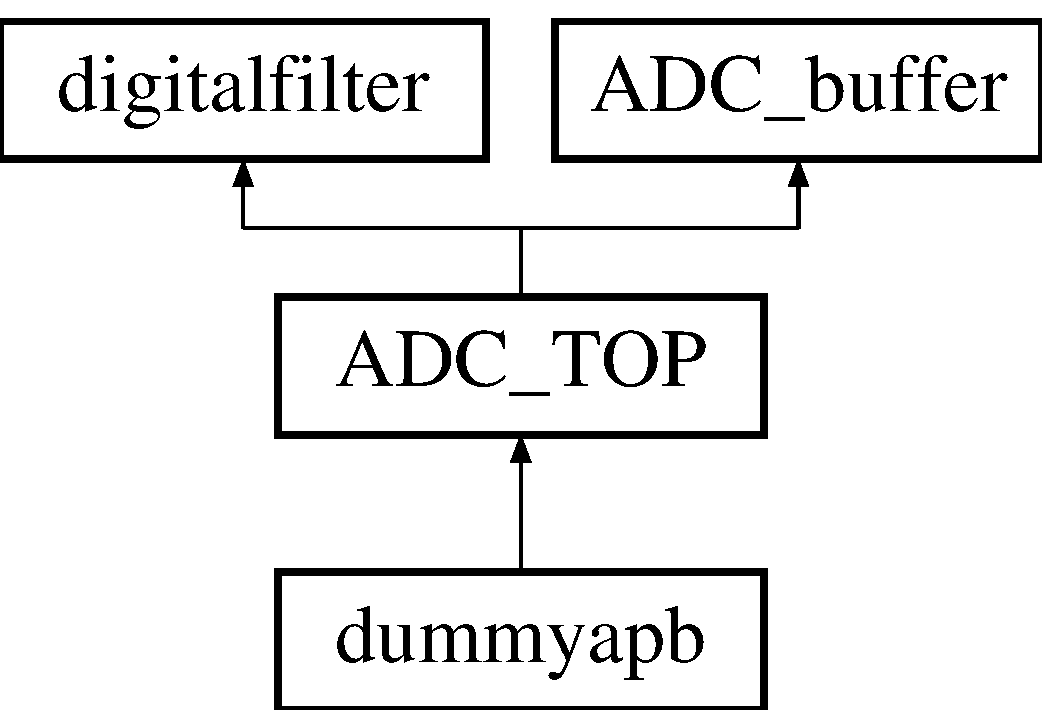
\includegraphics[height=3.000000cm]{classdummyapb}
\end{center}
\end{figure}
\subsection*{Entities}
\begin{DoxyCompactItemize}
\item 
\hyperlink{classdummyapb_1_1APB__interface}{A\-P\-B\-\_\-interface} architecture
\begin{DoxyCompactList}\small\item\em Architecture of the Dummy\-\_\-apb. \end{DoxyCompactList}\end{DoxyCompactItemize}
\subsection*{Libraries}
 \begin{DoxyCompactItemize}
\item 
\hypertarget{classdummyapb_ae4f03c286607f3181e16b9aa12d0c6d4}{\hyperlink{classdummyapb_ae4f03c286607f3181e16b9aa12d0c6d4}{I\-E\-E\-E} }\label{classdummyapb_ae4f03c286607f3181e16b9aa12d0c6d4}

\begin{DoxyCompactList}\small\item\em Use of standard library. \end{DoxyCompactList}\item 
\hypertarget{classdummyapb_a2306e6b22fb33ca087d2f1b289b10e28}{\hyperlink{classdummyapb_a2306e6b22fb33ca087d2f1b289b10e28}{grlib} }\label{classdummyapb_a2306e6b22fb33ca087d2f1b289b10e28}

\begin{DoxyCompactList}\small\item\em use of the G\-R\-L\-I\-B \end{DoxyCompactList}\end{DoxyCompactItemize}
\subsection*{Use Clauses}
 \begin{DoxyCompactItemize}
\item 
\hypertarget{classdummyapb_a68c233289eaf7d2601307bdd93b4c299}{\hyperlink{classdummyapb_a68c233289eaf7d2601307bdd93b4c299}{I\-E\-E\-E.\-S\-T\-D\-\_\-\-L\-O\-G\-I\-C\-\_\-1164.\-all}   }\label{classdummyapb_a68c233289eaf7d2601307bdd93b4c299}

\begin{DoxyCompactList}\small\item\em Use of standard logic arguments. \end{DoxyCompactList}\item 
\hypertarget{classdummyapb_a543ad46b77c6dc7048df8e72163d311d}{\hyperlink{classdummyapb_a543ad46b77c6dc7048df8e72163d311d}{grlib.\-amba.\-all}   }\label{classdummyapb_a543ad46b77c6dc7048df8e72163d311d}

\begin{DoxyCompactList}\small\item\em Use of the A\-M\-B\-A bus signals and constants. \end{DoxyCompactList}\item 
\hypertarget{classdummyapb_a8290b68c465332cd784781f7230e772d}{\hyperlink{classdummyapb_a8290b68c465332cd784781f7230e772d}{grlib.\-stdlib.\-all}   }\label{classdummyapb_a8290b68c465332cd784781f7230e772d}

\begin{DoxyCompactList}\small\item\em Use of standard G\-R\-L\-I\-B signals and constants. \end{DoxyCompactList}\item 
\hypertarget{classdummyapb_ad24672e694b1bed181a8b2813b132538}{\hyperlink{classdummyapb_ad24672e694b1bed181a8b2813b132538}{grlib.\-devices.\-all}   }\label{classdummyapb_ad24672e694b1bed181a8b2813b132538}

\begin{DoxyCompactList}\small\item\em use of G\-R\-L\-I\-B devices signals and constants \end{DoxyCompactList}\end{DoxyCompactItemize}
\subsection*{Generics}
 \begin{DoxyCompactItemize}
\item 
\hypertarget{classdummyapb_a5e1fd38c08cf4405b26bf887c5010e2b}{\hyperlink{classdummyapb_a5e1fd38c08cf4405b26bf887c5010e2b}{pindex} {\bfseries {\bfseries \textcolor{comment}{integer}\textcolor{vhdlchar}{ }\textcolor{vhdlchar}{\-:}\textcolor{vhdlchar}{=}\textcolor{vhdlchar}{ } \textcolor{vhdldigit}{0} \textcolor{vhdlchar}{ }}}}\label{classdummyapb_a5e1fd38c08cf4405b26bf887c5010e2b}

\begin{DoxyCompactList}\small\item\em Slave index. \end{DoxyCompactList}\item 
\hypertarget{classdummyapb_a1c4c90775fe1a0af1ff79546ceb2f9c2}{\hyperlink{classdummyapb_a1c4c90775fe1a0af1ff79546ceb2f9c2}{paddr} {\bfseries {\bfseries \textcolor{comment}{integer}\textcolor{vhdlchar}{ }\textcolor{vhdlchar}{\-:}\textcolor{vhdlchar}{=}\textcolor{vhdlchar}{ } \textcolor{vhdldigit}{0} \textcolor{vhdlchar}{ }}}}\label{classdummyapb_a1c4c90775fe1a0af1ff79546ceb2f9c2}

\begin{DoxyCompactList}\small\item\em Address of the A\-P\-B bank. \end{DoxyCompactList}\item 
\hypertarget{classdummyapb_ae4b21043dd0ec623e5b8ed1cbe9db7b5}{\hyperlink{classdummyapb_ae4b21043dd0ec623e5b8ed1cbe9db7b5}{pmask} {\bfseries {\bfseries \textcolor{comment}{integer}\textcolor{vhdlchar}{ }\textcolor{vhdlchar}{\-:}\textcolor{vhdlchar}{=}\textcolor{vhdlchar}{ } \textcolor{vhdldigit}{16\#fff\#} \textcolor{vhdlchar}{ }}}}\label{classdummyapb_ae4b21043dd0ec623e5b8ed1cbe9db7b5}

\begin{DoxyCompactList}\small\item\em Address range. \end{DoxyCompactList}\end{DoxyCompactItemize}
\subsection*{Ports}
 \begin{DoxyCompactItemize}
\item 
\hypertarget{classdummyapb_a8fb8388e1e2f3ac69332573f5909b4e8}{\hyperlink{classdummyapb_a8fb8388e1e2f3ac69332573f5909b4e8}{rstn}  {\bfseries {\bfseries \textcolor{vhdlkeyword}{in}\textcolor{vhdlchar}{ }}} {\bfseries \textcolor{comment}{std\-\_\-ulogic}\textcolor{vhdlchar}{ }} }\label{classdummyapb_a8fb8388e1e2f3ac69332573f5909b4e8}

\begin{DoxyCompactList}\small\item\em Global reset, active low. \end{DoxyCompactList}\item 
\hypertarget{classdummyapb_af1c59ef8e5ba3edeeb313b4be18d7d8a}{\hyperlink{classdummyapb_af1c59ef8e5ba3edeeb313b4be18d7d8a}{clk}  {\bfseries {\bfseries \textcolor{vhdlkeyword}{in}\textcolor{vhdlchar}{ }}} {\bfseries \textcolor{comment}{std\-\_\-ulogic}\textcolor{vhdlchar}{ }} }\label{classdummyapb_af1c59ef8e5ba3edeeb313b4be18d7d8a}

\begin{DoxyCompactList}\small\item\em Clock at the bus speed of 50 M\-Hz. \end{DoxyCompactList}\item 
\hypertarget{classdummyapb_acfb2eee7a14b6192c7945bbb7ba640fa}{\hyperlink{classdummyapb_acfb2eee7a14b6192c7945bbb7ba640fa}{clk100}  {\bfseries {\bfseries \textcolor{vhdlkeyword}{in}\textcolor{vhdlchar}{ }}} {\bfseries \textcolor{comment}{std\-\_\-ulogic}\textcolor{vhdlchar}{ }} }\label{classdummyapb_acfb2eee7a14b6192c7945bbb7ba640fa}

\begin{DoxyCompactList}\small\item\em Clock at 100 M\-Hz for certain speed dependent modules. \end{DoxyCompactList}\item 
\hypertarget{classdummyapb_af2205ffee98e5aeaa144186159740393}{\hyperlink{classdummyapb_af2205ffee98e5aeaa144186159740393}{vauxp3}  {\bfseries {\bfseries \textcolor{vhdlkeyword}{in}\textcolor{vhdlchar}{ }}} {\bfseries \textcolor{comment}{S\-T\-D\-\_\-\-L\-O\-G\-I\-C}\textcolor{vhdlchar}{ }} }\label{classdummyapb_af2205ffee98e5aeaa144186159740393}

\begin{DoxyCompactList}\small\item\em X\-A\-D\-C related signal. \end{DoxyCompactList}\item 
\hypertarget{classdummyapb_a3d034bd2912bb721a5bd221c185c5c99}{\hyperlink{classdummyapb_a3d034bd2912bb721a5bd221c185c5c99}{vauxn3}  {\bfseries {\bfseries \textcolor{vhdlkeyword}{in}\textcolor{vhdlchar}{ }}} {\bfseries \textcolor{comment}{S\-T\-D\-\_\-\-L\-O\-G\-I\-C}\textcolor{vhdlchar}{ }} }\label{classdummyapb_a3d034bd2912bb721a5bd221c185c5c99}

\begin{DoxyCompactList}\small\item\em X\-A\-D\-C related signal. \end{DoxyCompactList}\item 
\hypertarget{classdummyapb_abd7039100e504d8f92a35144147f07d7}{\hyperlink{classdummyapb_abd7039100e504d8f92a35144147f07d7}{apbi}  {\bfseries {\bfseries \textcolor{vhdlkeyword}{in}\textcolor{vhdlchar}{ }}} {\bfseries \textcolor{vhdlchar}{apb\-\_\-slv\-\_\-in\-\_\-type}\textcolor{vhdlchar}{ }} }\label{classdummyapb_abd7039100e504d8f92a35144147f07d7}

\begin{DoxyCompactList}\small\item\em A\-P\-B slave inputs. \end{DoxyCompactList}\item 
\hypertarget{classdummyapb_a7e895c34eed119599f289452433acbf2}{\hyperlink{classdummyapb_a7e895c34eed119599f289452433acbf2}{apbo}  {\bfseries {\bfseries \textcolor{vhdlkeyword}{out}\textcolor{vhdlchar}{ }}} {\bfseries \textcolor{vhdlchar}{apb\-\_\-slv\-\_\-out\-\_\-type}\textcolor{vhdlchar}{ }} }\label{classdummyapb_a7e895c34eed119599f289452433acbf2}

\begin{DoxyCompactList}\small\item\em A\-P\-B slave outputs. \end{DoxyCompactList}\item 
\hypertarget{classdummyapb_ad82a959b5a4a639e7c0a09e6b1e31705}{\hyperlink{classdummyapb_ad82a959b5a4a639e7c0a09e6b1e31705}{spi\-Sclk}  {\bfseries {\bfseries \textcolor{vhdlkeyword}{out}\textcolor{vhdlchar}{ }}} {\bfseries \textcolor{comment}{std\-\_\-logic}\textcolor{vhdlchar}{ }} }\label{classdummyapb_ad82a959b5a4a639e7c0a09e6b1e31705}

\begin{DoxyCompactList}\small\item\em Serial clock for D\-A\-C S\-P\-I. \end{DoxyCompactList}\item 
\hypertarget{classdummyapb_a77f854eda2e8d157ccc5d2d08e8ecfb7}{\hyperlink{classdummyapb_a77f854eda2e8d157ccc5d2d08e8ecfb7}{spi\-Din}  {\bfseries {\bfseries \textcolor{vhdlkeyword}{out}\textcolor{vhdlchar}{ }}} {\bfseries \textcolor{comment}{std\-\_\-logic}\textcolor{vhdlchar}{ }} }\label{classdummyapb_a77f854eda2e8d157ccc5d2d08e8ecfb7}

\begin{DoxyCompactList}\small\item\em Data signal for D\-A\-C S\-P\-I. \end{DoxyCompactList}\item 
\hypertarget{classdummyapb_ae9d5788ea215a9d9dd1b8b43e977d582}{\hyperlink{classdummyapb_ae9d5788ea215a9d9dd1b8b43e977d582}{spi\-Nsync}  {\bfseries {\bfseries \textcolor{vhdlkeyword}{out}\textcolor{vhdlchar}{ }}} {\bfseries \textcolor{comment}{std\-\_\-logic}\textcolor{vhdlchar}{ }} }\label{classdummyapb_ae9d5788ea215a9d9dd1b8b43e977d582}

\begin{DoxyCompactList}\small\item\em Sync signal for D\-A\-C S\-P\-I. \end{DoxyCompactList}\end{DoxyCompactItemize}


\subsection{Detailed Description}
This component gathers all the sub-\/modules needed for communication with A\-D\-C and D\-A\-C. It also supplies an interface to the A\-P\-B bus. 

The documentation for this class was generated from the following file\-:\begin{DoxyCompactItemize}
\item 
\hyperlink{dummyapb_8vhd}{dummyapb.\-vhd}\end{DoxyCompactItemize}

\hypertarget{classbounce__filter_1_1filter__bounce}{\section{filter\-\_\-bounce Architecture Reference}
\label{classbounce__filter_1_1filter__bounce}\index{filter\-\_\-bounce@{filter\-\_\-bounce}}
}


Architecture of the \hyperlink{classbounce__filter}{bounce\-\_\-filter}.  


\subsection*{Processes}
 \begin{DoxyCompactItemize}
\item 
\hypertarget{classbounce__filter_1_1filter__bounce_a68c86990d057b8db759843e21da325c7}{\hyperlink{classbounce__filter_1_1filter__bounce_a68c86990d057b8db759843e21da325c7}{P\-R\-O\-C\-E\-S\-S\-\_\-2}{\bfseries  ( {\bfseries {\bfseries \hyperlink{classbounce__filter_aba021aec4b477b89079bb58ccadcc67e}{rstn}} \textcolor{vhdlchar}{ }\textcolor{vhdlchar}{ }\textcolor{vhdlchar}{ }} , {\bfseries {\bfseries \hyperlink{classbounce__filter_a8120037e0ee47c35ba2d79242209c72e}{clk}} \textcolor{vhdlchar}{ }} )}}\label{classbounce__filter_1_1filter__bounce_a68c86990d057b8db759843e21da325c7}

\end{DoxyCompactItemize}
\subsection*{Signals}
 \begin{DoxyCompactItemize}
\item 
\hypertarget{classbounce__filter_1_1filter__bounce_a91ed0cb5ab66576a11c5a2a0de9a88af}{\hyperlink{classbounce__filter_1_1filter__bounce_a91ed0cb5ab66576a11c5a2a0de9a88af}{cnt} {\bfseries \textcolor{comment}{unsigned}\textcolor{vhdlchar}{ }\textcolor{vhdlchar}{(}\textcolor{vhdlchar}{ }\textcolor{vhdlchar}{ }{\bfseries \hyperlink{classbounce__filter_a5df2a2aceb759129bf8abccdc30aec13}{counterbits}} \textcolor{vhdlchar}{ }\textcolor{vhdlchar}{-\/}\textcolor{vhdlchar}{ } \textcolor{vhdldigit}{1} \textcolor{vhdlchar}{ }\textcolor{vhdlchar}{ }\textcolor{vhdlchar}{ }\textcolor{vhdlkeyword}{downto}\textcolor{vhdlchar}{ }\textcolor{vhdlchar}{ }\textcolor{vhdlchar}{ } \textcolor{vhdldigit}{0} \textcolor{vhdlchar}{ }\textcolor{vhdlchar}{)}\textcolor{vhdlchar}{ }} }\label{classbounce__filter_1_1filter__bounce_a91ed0cb5ab66576a11c5a2a0de9a88af}

\begin{DoxyCompactList}\small\item\em A counter signal, the size is defined by the generic. \end{DoxyCompactList}\item 
\hypertarget{classbounce__filter_1_1filter__bounce_af1b9cebedbee1076cdea82a2084c53d7}{\hyperlink{classbounce__filter_1_1filter__bounce_af1b9cebedbee1076cdea82a2084c53d7}{last\-\_\-button\-\_\-in} {\bfseries \textcolor{comment}{std\-\_\-logic}\textcolor{vhdlchar}{ }} }\label{classbounce__filter_1_1filter__bounce_af1b9cebedbee1076cdea82a2084c53d7}

\begin{DoxyCompactList}\small\item\em A signal to indicate the last state of the button in. \end{DoxyCompactList}\item 
\hypertarget{classbounce__filter_1_1filter__bounce_a42b551e04fcfc5a7c7ec2b57a2879dc0}{\hyperlink{classbounce__filter_1_1filter__bounce_a42b551e04fcfc5a7c7ec2b57a2879dc0}{button\-\_\-out\-\_\-buff} {\bfseries \textcolor{comment}{S\-T\-D\-\_\-\-L\-O\-G\-I\-C}\textcolor{vhdlchar}{ }} }\label{classbounce__filter_1_1filter__bounce_a42b551e04fcfc5a7c7ec2b57a2879dc0}

\begin{DoxyCompactList}\small\item\em A buffered value of the output to determine if the output changes from low to high or high to low. \end{DoxyCompactList}\end{DoxyCompactItemize}


\subsection{Detailed Description}
Architecture of the \hyperlink{classbounce__filter}{bounce\-\_\-filter}. 

This component stabilizes an input signal using a counter. This counter can be set with the generic. If the signal changed during the counting the counter resets to 0. 

The documentation for this class was generated from the following file\-:\begin{DoxyCompactItemize}
\item 
\hyperlink{bounce__filter_8vhd}{bounce\-\_\-filter.\-vhd}\end{DoxyCompactItemize}

\hypertarget{classdigitalfilter_1_1FIR__filter}{\section{F\-I\-R\-\_\-filter Architecture Reference}
\label{classdigitalfilter_1_1FIR__filter}\index{F\-I\-R\-\_\-filter@{F\-I\-R\-\_\-filter}}
}


digitalfilter  


\subsection*{Processes}
 \begin{DoxyCompactItemize}
\item 
\hypertarget{classdigitalfilter_1_1FIR__filter_a7e91e75a2c6c203fc15a2560e69701cc}{\hyperlink{classdigitalfilter_1_1FIR__filter_a7e91e75a2c6c203fc15a2560e69701cc}{P\-R\-O\-C\-E\-S\-S\-\_\-7}{\bfseries  ( {\bfseries {\bfseries \hyperlink{classdigitalfilter_aae5de5c5aebf7b54ecd36feaba217215}{reset}} \textcolor{vhdlchar}{ }\textcolor{vhdlchar}{ }\textcolor{vhdlchar}{ }} , {\bfseries {\bfseries \hyperlink{classdigitalfilter_a8120037e0ee47c35ba2d79242209c72e}{clk}} \textcolor{vhdlchar}{ }} )}}\label{classdigitalfilter_1_1FIR__filter_a7e91e75a2c6c203fc15a2560e69701cc}

\begin{DoxyCompactList}\small\item\em The filter parameters. \end{DoxyCompactList}\end{DoxyCompactItemize}
\subsection*{Constants}
 \begin{DoxyCompactItemize}
\item 
\hypertarget{classdigitalfilter_1_1FIR__filter_a25eec2bc9f015a7c1413a1668e3b9fcf}{\hyperlink{classdigitalfilter_1_1FIR__filter_a25eec2bc9f015a7c1413a1668e3b9fcf}{F\-I\-L\-T\-E\-R\-\_\-\-P\-A\-R\-A\-M\-E\-T\-E\-R\-S} {\bfseries \textcolor{vhdlchar}{parameter\-\_\-array\-\_\-type}\textcolor{vhdlchar}{ }\textcolor{vhdlchar}{ }\textcolor{vhdlchar}{\-:}\textcolor{vhdlchar}{=}\textcolor{vhdlchar}{ }\textcolor{vhdlchar}{ }\textcolor{vhdlchar}{(}\textcolor{vhdlchar}{ }\textcolor{vhdlchar}{ }{\bfseries \hyperlink{classdigitalfilter_a8c5602ac7769fa0806595aa864d2134b}{x}} \textcolor{vhdlchar}{ }\textcolor{keyword}{\char`\"{} 0041b1f5 \char`\"{}}\textcolor{vhdlchar}{ }\textcolor{vhdlchar}{,}\textcolor{vhdlchar}{ }\textcolor{vhdlchar}{ }{\bfseries \hyperlink{classdigitalfilter_a8c5602ac7769fa0806595aa864d2134b}{x}} \textcolor{vhdlchar}{ }\textcolor{keyword}{\char`\"{} 00462ce8 \char`\"{}}\textcolor{vhdlchar}{ }\textcolor{vhdlchar}{,}\textcolor{vhdlchar}{ }\textcolor{vhdlchar}{ }{\bfseries \hyperlink{classdigitalfilter_a8c5602ac7769fa0806595aa864d2134b}{x}} \textcolor{vhdlchar}{ }\textcolor{keyword}{\char`\"{} 00693e0c \char`\"{}}\textcolor{vhdlchar}{ }\textcolor{vhdlchar}{,}\textcolor{vhdlchar}{ }\textcolor{vhdlchar}{ }{\bfseries \hyperlink{classdigitalfilter_a8c5602ac7769fa0806595aa864d2134b}{x}} \textcolor{vhdlchar}{ }\textcolor{keyword}{\char`\"{} 00958f2e \char`\"{}}\textcolor{vhdlchar}{ }\textcolor{vhdlchar}{,}\textcolor{vhdlchar}{ }\textcolor{vhdlchar}{ }{\bfseries \hyperlink{classdigitalfilter_a8c5602ac7769fa0806595aa864d2134b}{x}} \textcolor{vhdlchar}{ }\textcolor{keyword}{\char`\"{} 00cbd646 \char`\"{}}\textcolor{vhdlchar}{ }\textcolor{vhdlchar}{,}\textcolor{vhdlchar}{ }\textcolor{vhdlchar}{ }{\bfseries \hyperlink{classdigitalfilter_a8c5602ac7769fa0806595aa864d2134b}{x}} \textcolor{vhdlchar}{ }\textcolor{keyword}{\char`\"{} 010c8add \char`\"{}}\textcolor{vhdlchar}{ }\textcolor{vhdlchar}{,}\textcolor{vhdlchar}{ }\textcolor{vhdlchar}{ }{\bfseries \hyperlink{classdigitalfilter_a8c5602ac7769fa0806595aa864d2134b}{x}} \textcolor{vhdlchar}{ }\textcolor{keyword}{\char`\"{} 0157b719 \char`\"{}}\textcolor{vhdlchar}{ }\textcolor{vhdlchar}{,}\textcolor{vhdlchar}{ }\textcolor{vhdlchar}{ }{\bfseries \hyperlink{classdigitalfilter_a8c5602ac7769fa0806595aa864d2134b}{x}} \textcolor{vhdlchar}{ }\textcolor{keyword}{\char`\"{} 01acf299 \char`\"{}}\textcolor{vhdlchar}{ }\textcolor{vhdlchar}{,}\textcolor{vhdlchar}{ }\textcolor{vhdlchar}{ }{\bfseries \hyperlink{classdigitalfilter_a8c5602ac7769fa0806595aa864d2134b}{x}} \textcolor{vhdlchar}{ }\textcolor{keyword}{\char`\"{} 020b3c83 \char`\"{}}\textcolor{vhdlchar}{ }\textcolor{vhdlchar}{,}\textcolor{vhdlchar}{ }\textcolor{vhdlchar}{ }{\bfseries \hyperlink{classdigitalfilter_a8c5602ac7769fa0806595aa864d2134b}{x}} \textcolor{vhdlchar}{ }\textcolor{keyword}{\char`\"{} 0270fe9f \char`\"{}}\textcolor{vhdlchar}{ }\textcolor{vhdlchar}{,}\textcolor{vhdlchar}{ }\textcolor{vhdlchar}{ }{\bfseries \hyperlink{classdigitalfilter_a8c5602ac7769fa0806595aa864d2134b}{x}} \textcolor{vhdlchar}{ }\textcolor{keyword}{\char`\"{} 02dbf43d \char`\"{}}\textcolor{vhdlchar}{ }\textcolor{vhdlchar}{,}\textcolor{vhdlchar}{ }\textcolor{vhdlchar}{ }{\bfseries \hyperlink{classdigitalfilter_a8c5602ac7769fa0806595aa864d2134b}{x}} \textcolor{vhdlchar}{ }\textcolor{keyword}{\char`\"{} 03492ca7 \char`\"{}}\textcolor{vhdlchar}{ }\textcolor{vhdlchar}{,}\textcolor{vhdlchar}{ }\textcolor{vhdlchar}{ }{\bfseries \hyperlink{classdigitalfilter_a8c5602ac7769fa0806595aa864d2134b}{x}} \textcolor{vhdlchar}{ }\textcolor{keyword}{\char`\"{} 03b4f47c \char`\"{}}\textcolor{vhdlchar}{ }\textcolor{vhdlchar}{,}\textcolor{vhdlchar}{ }\textcolor{vhdlchar}{ }{\bfseries \hyperlink{classdigitalfilter_a8c5602ac7769fa0806595aa864d2134b}{x}} \textcolor{vhdlchar}{ }\textcolor{keyword}{\char`\"{} 041af631 \char`\"{}}\textcolor{vhdlchar}{ }\textcolor{vhdlchar}{,}\textcolor{vhdlchar}{ }\textcolor{vhdlchar}{ }{\bfseries \hyperlink{classdigitalfilter_a8c5602ac7769fa0806595aa864d2134b}{x}} \textcolor{vhdlchar}{ }\textcolor{keyword}{\char`\"{} 047641dc \char`\"{}}\textcolor{vhdlchar}{ }\textcolor{vhdlchar}{,}\textcolor{vhdlchar}{ }\textcolor{vhdlchar}{ }{\bfseries \hyperlink{classdigitalfilter_a8c5602ac7769fa0806595aa864d2134b}{x}} \textcolor{vhdlchar}{ }\textcolor{keyword}{\char`\"{} 04c16e65 \char`\"{}}\textcolor{vhdlchar}{ }\textcolor{vhdlchar}{,}\textcolor{vhdlchar}{ }\textcolor{vhdlchar}{ }{\bfseries \hyperlink{classdigitalfilter_a8c5602ac7769fa0806595aa864d2134b}{x}} \textcolor{vhdlchar}{ }\textcolor{keyword}{\char`\"{} 04f69e6e \char`\"{}}\textcolor{vhdlchar}{ }\textcolor{vhdlchar}{,}\textcolor{vhdlchar}{ }\textcolor{vhdlchar}{ }{\bfseries \hyperlink{classdigitalfilter_a8c5602ac7769fa0806595aa864d2134b}{x}} \textcolor{vhdlchar}{ }\textcolor{keyword}{\char`\"{} 050fc1f9 \char`\"{}}\textcolor{vhdlchar}{ }\textcolor{vhdlchar}{,}\textcolor{vhdlchar}{ }\textcolor{vhdlchar}{ }{\bfseries \hyperlink{classdigitalfilter_a8c5602ac7769fa0806595aa864d2134b}{x}} \textcolor{vhdlchar}{ }\textcolor{keyword}{\char`\"{} 0506d3c5 \char`\"{}}\textcolor{vhdlchar}{ }\textcolor{vhdlchar}{,}\textcolor{vhdlchar}{ }\textcolor{vhdlchar}{ }{\bfseries \hyperlink{classdigitalfilter_a8c5602ac7769fa0806595aa864d2134b}{x}} \textcolor{vhdlchar}{ }\textcolor{keyword}{\char`\"{} 04d60dd4 \char`\"{}}\textcolor{vhdlchar}{ }\textcolor{vhdlchar}{,}\textcolor{vhdlchar}{ }\textcolor{vhdlchar}{ }{\bfseries \hyperlink{classdigitalfilter_a8c5602ac7769fa0806595aa864d2134b}{x}} \textcolor{vhdlchar}{ }\textcolor{keyword}{\char`\"{} 0477ff3a \char`\"{}}\textcolor{vhdlchar}{ }\textcolor{vhdlchar}{,}\textcolor{vhdlchar}{ }\textcolor{vhdlchar}{ }{\bfseries \hyperlink{classdigitalfilter_a8c5602ac7769fa0806595aa864d2134b}{x}} \textcolor{vhdlchar}{ }\textcolor{keyword}{\char`\"{} 03e81aa5 \char`\"{}}\textcolor{vhdlchar}{ }\textcolor{vhdlchar}{,}\textcolor{vhdlchar}{ }\textcolor{vhdlchar}{ }{\bfseries \hyperlink{classdigitalfilter_a8c5602ac7769fa0806595aa864d2134b}{x}} \textcolor{vhdlchar}{ }\textcolor{keyword}{\char`\"{} 0322e43a \char`\"{}}\textcolor{vhdlchar}{ }\textcolor{vhdlchar}{,}\textcolor{vhdlchar}{ }\textcolor{vhdlchar}{ }{\bfseries \hyperlink{classdigitalfilter_a8c5602ac7769fa0806595aa864d2134b}{x}} \textcolor{vhdlchar}{ }\textcolor{keyword}{\char`\"{} 0225ed51 \char`\"{}}\textcolor{vhdlchar}{ }\textcolor{vhdlchar}{,}\textcolor{vhdlchar}{ }\textcolor{vhdlchar}{ }{\bfseries \hyperlink{classdigitalfilter_a8c5602ac7769fa0806595aa864d2134b}{x}} \textcolor{vhdlchar}{ }\textcolor{keyword}{\char`\"{} 00f0a718 \char`\"{}}\textcolor{vhdlchar}{ }\textcolor{vhdlchar}{,}\textcolor{vhdlchar}{ }\textcolor{vhdlchar}{ }{\bfseries \hyperlink{classdigitalfilter_a8c5602ac7769fa0806595aa864d2134b}{x}} \textcolor{vhdlchar}{ }\textcolor{keyword}{\char`\"{} ff841059 \char`\"{}}\textcolor{vhdlchar}{ }\textcolor{vhdlchar}{,}\textcolor{vhdlchar}{ }\textcolor{vhdlchar}{ }{\bfseries \hyperlink{classdigitalfilter_a8c5602ac7769fa0806595aa864d2134b}{x}} \textcolor{vhdlchar}{ }\textcolor{keyword}{\char`\"{} fde34b3b \char`\"{}}\textcolor{vhdlchar}{ }\textcolor{vhdlchar}{,}\textcolor{vhdlchar}{ }\textcolor{vhdlchar}{ }{\bfseries \hyperlink{classdigitalfilter_a8c5602ac7769fa0806595aa864d2134b}{x}} \textcolor{vhdlchar}{ }\textcolor{keyword}{\char`\"{} fc13990e \char`\"{}}\textcolor{vhdlchar}{ }\textcolor{vhdlchar}{,}\textcolor{vhdlchar}{ }\textcolor{vhdlchar}{ }{\bfseries \hyperlink{classdigitalfilter_a8c5602ac7769fa0806595aa864d2134b}{x}} \textcolor{vhdlchar}{ }\textcolor{keyword}{\char`\"{} fa1c76b5 \char`\"{}}\textcolor{vhdlchar}{ }\textcolor{vhdlchar}{,}\textcolor{vhdlchar}{ }\textcolor{vhdlchar}{ }{\bfseries \hyperlink{classdigitalfilter_a8c5602ac7769fa0806595aa864d2134b}{x}} \textcolor{vhdlchar}{ }\textcolor{keyword}{\char`\"{} f807b848 \char`\"{}}\textcolor{vhdlchar}{ }\textcolor{vhdlchar}{,}\textcolor{vhdlchar}{ }\textcolor{vhdlchar}{ }{\bfseries \hyperlink{classdigitalfilter_a8c5602ac7769fa0806595aa864d2134b}{x}} \textcolor{vhdlchar}{ }\textcolor{keyword}{\char`\"{} f5e16719 \char`\"{}}\textcolor{vhdlchar}{ }\textcolor{vhdlchar}{,}\textcolor{vhdlchar}{ }\textcolor{vhdlchar}{ }{\bfseries \hyperlink{classdigitalfilter_a8c5602ac7769fa0806595aa864d2134b}{x}} \textcolor{vhdlchar}{ }\textcolor{keyword}{\char`\"{} f3b7b517 \char`\"{}}\textcolor{vhdlchar}{ }\textcolor{vhdlchar}{,}\textcolor{vhdlchar}{ }\textcolor{vhdlchar}{ }{\bfseries \hyperlink{classdigitalfilter_a8c5602ac7769fa0806595aa864d2134b}{x}} \textcolor{vhdlchar}{ }\textcolor{keyword}{\char`\"{} f19ab76c \char`\"{}}\textcolor{vhdlchar}{ }\textcolor{vhdlchar}{,}\textcolor{vhdlchar}{ }\textcolor{vhdlchar}{ }{\bfseries \hyperlink{classdigitalfilter_a8c5602ac7769fa0806595aa864d2134b}{x}} \textcolor{vhdlchar}{ }\textcolor{keyword}{\char`\"{} ef9c3525 \char`\"{}}\textcolor{vhdlchar}{ }\textcolor{vhdlchar}{,}\textcolor{vhdlchar}{ }\textcolor{vhdlchar}{ }{\bfseries \hyperlink{classdigitalfilter_a8c5602ac7769fa0806595aa864d2134b}{x}} \textcolor{vhdlchar}{ }\textcolor{keyword}{\char`\"{} edcf338b \char`\"{}}\textcolor{vhdlchar}{ }\textcolor{vhdlchar}{,}\textcolor{vhdlchar}{ }\textcolor{vhdlchar}{ }{\bfseries \hyperlink{classdigitalfilter_a8c5602ac7769fa0806595aa864d2134b}{x}} \textcolor{vhdlchar}{ }\textcolor{keyword}{\char`\"{} ec479930 \char`\"{}}\textcolor{vhdlchar}{ }\textcolor{vhdlchar}{,}\textcolor{vhdlchar}{ }\textcolor{vhdlchar}{ }{\bfseries \hyperlink{classdigitalfilter_a8c5602ac7769fa0806595aa864d2134b}{x}} \textcolor{vhdlchar}{ }\textcolor{keyword}{\char`\"{} eb199d89 \char`\"{}}\textcolor{vhdlchar}{ }\textcolor{vhdlchar}{,}\textcolor{vhdlchar}{ }\textcolor{vhdlchar}{ }{\bfseries \hyperlink{classdigitalfilter_a8c5602ac7769fa0806595aa864d2134b}{x}} \textcolor{vhdlchar}{ }\textcolor{keyword}{\char`\"{} ea5952f6 \char`\"{}}\textcolor{vhdlchar}{ }\textcolor{vhdlchar}{,}\textcolor{vhdlchar}{ }\textcolor{vhdlchar}{ }{\bfseries \hyperlink{classdigitalfilter_a8c5602ac7769fa0806595aa864d2134b}{x}} \textcolor{vhdlchar}{ }\textcolor{keyword}{\char`\"{} ea19f88c \char`\"{}}\textcolor{vhdlchar}{ }\textcolor{vhdlchar}{,}\textcolor{vhdlchar}{ }\textcolor{vhdlchar}{ }{\bfseries \hyperlink{classdigitalfilter_a8c5602ac7769fa0806595aa864d2134b}{x}} \textcolor{vhdlchar}{ }\textcolor{keyword}{\char`\"{} ea6d6b27 \char`\"{}}\textcolor{vhdlchar}{ }\textcolor{vhdlchar}{,}\textcolor{vhdlchar}{ }\textcolor{vhdlchar}{ }{\bfseries \hyperlink{classdigitalfilter_a8c5602ac7769fa0806595aa864d2134b}{x}} \textcolor{vhdlchar}{ }\textcolor{keyword}{\char`\"{} eb6387d1 \char`\"{}}\textcolor{vhdlchar}{ }\textcolor{vhdlchar}{,}\textcolor{vhdlchar}{ }\textcolor{vhdlchar}{ }{\bfseries \hyperlink{classdigitalfilter_a8c5602ac7769fa0806595aa864d2134b}{x}} \textcolor{vhdlchar}{ }\textcolor{keyword}{\char`\"{} ed099a31 \char`\"{}}\textcolor{vhdlchar}{ }\textcolor{vhdlchar}{,}\textcolor{vhdlchar}{ }\textcolor{vhdlchar}{ }{\bfseries \hyperlink{classdigitalfilter_a8c5602ac7769fa0806595aa864d2134b}{x}} \textcolor{vhdlchar}{ }\textcolor{keyword}{\char`\"{} ef69b5fa \char`\"{}}\textcolor{vhdlchar}{ }\textcolor{vhdlchar}{,}\textcolor{vhdlchar}{ }\textcolor{vhdlchar}{ }{\bfseries \hyperlink{classdigitalfilter_a8c5602ac7769fa0806595aa864d2134b}{x}} \textcolor{vhdlchar}{ }\textcolor{keyword}{\char`\"{} f28a5e48 \char`\"{}}\textcolor{vhdlchar}{ }\textcolor{vhdlchar}{,}\textcolor{vhdlchar}{ }\textcolor{vhdlchar}{ }{\bfseries \hyperlink{classdigitalfilter_a8c5602ac7769fa0806595aa864d2134b}{x}} \textcolor{vhdlchar}{ }\textcolor{keyword}{\char`\"{} f66df637 \char`\"{}}\textcolor{vhdlchar}{ }\textcolor{vhdlchar}{,}\textcolor{vhdlchar}{ }\textcolor{vhdlchar}{ }{\bfseries \hyperlink{classdigitalfilter_a8c5602ac7769fa0806595aa864d2134b}{x}} \textcolor{vhdlchar}{ }\textcolor{keyword}{\char`\"{} fb127d21 \char`\"{}}\textcolor{vhdlchar}{ }\textcolor{vhdlchar}{,}\textcolor{vhdlchar}{ }\textcolor{vhdlchar}{ }{\bfseries \hyperlink{classdigitalfilter_a8c5602ac7769fa0806595aa864d2134b}{x}} \textcolor{vhdlchar}{ }\textcolor{keyword}{\char`\"{} 00715beb \char`\"{}}\textcolor{vhdlchar}{ }\textcolor{vhdlchar}{,}\textcolor{vhdlchar}{ }\textcolor{vhdlchar}{ }{\bfseries \hyperlink{classdigitalfilter_a8c5602ac7769fa0806595aa864d2134b}{x}} \textcolor{vhdlchar}{ }\textcolor{keyword}{\char`\"{} 067f373a \char`\"{}}\textcolor{vhdlchar}{ }\textcolor{vhdlchar}{,}\textcolor{vhdlchar}{ }\textcolor{vhdlchar}{ }{\bfseries \hyperlink{classdigitalfilter_a8c5602ac7769fa0806595aa864d2134b}{x}} \textcolor{vhdlchar}{ }\textcolor{keyword}{\char`\"{} 0d2c0bab \char`\"{}}\textcolor{vhdlchar}{ }\textcolor{vhdlchar}{,}\textcolor{vhdlchar}{ }\textcolor{vhdlchar}{ }{\bfseries \hyperlink{classdigitalfilter_a8c5602ac7769fa0806595aa864d2134b}{x}} \textcolor{vhdlchar}{ }\textcolor{keyword}{\char`\"{} 1463500e \char`\"{}}\textcolor{vhdlchar}{ }\textcolor{vhdlchar}{,}\textcolor{vhdlchar}{ }\textcolor{vhdlchar}{ }{\bfseries \hyperlink{classdigitalfilter_a8c5602ac7769fa0806595aa864d2134b}{x}} \textcolor{vhdlchar}{ }\textcolor{keyword}{\char`\"{} 1c0c3948 \char`\"{}}\textcolor{vhdlchar}{ }\textcolor{vhdlchar}{,}\textcolor{vhdlchar}{ }\textcolor{vhdlchar}{ }{\bfseries \hyperlink{classdigitalfilter_a8c5602ac7769fa0806595aa864d2134b}{x}} \textcolor{vhdlchar}{ }\textcolor{keyword}{\char`\"{} 240a3bae \char`\"{}}\textcolor{vhdlchar}{ }\textcolor{vhdlchar}{,}\textcolor{vhdlchar}{ }\textcolor{vhdlchar}{ }{\bfseries \hyperlink{classdigitalfilter_a8c5602ac7769fa0806595aa864d2134b}{x}} \textcolor{vhdlchar}{ }\textcolor{keyword}{\char`\"{} 2c3d832f \char`\"{}}\textcolor{vhdlchar}{ }\textcolor{vhdlchar}{,}\textcolor{vhdlchar}{ }\textcolor{vhdlchar}{ }{\bfseries \hyperlink{classdigitalfilter_a8c5602ac7769fa0806595aa864d2134b}{x}} \textcolor{vhdlchar}{ }\textcolor{keyword}{\char`\"{} 3483b0e0 \char`\"{}}\textcolor{vhdlchar}{ }\textcolor{vhdlchar}{,}\textcolor{vhdlchar}{ }\textcolor{vhdlchar}{ }{\bfseries \hyperlink{classdigitalfilter_a8c5602ac7769fa0806595aa864d2134b}{x}} \textcolor{vhdlchar}{ }\textcolor{keyword}{\char`\"{} 3cb88747 \char`\"{}}\textcolor{vhdlchar}{ }\textcolor{vhdlchar}{,}\textcolor{vhdlchar}{ }\textcolor{vhdlchar}{ }{\bfseries \hyperlink{classdigitalfilter_a8c5602ac7769fa0806595aa864d2134b}{x}} \textcolor{vhdlchar}{ }\textcolor{keyword}{\char`\"{} 44b6d486 \char`\"{}}\textcolor{vhdlchar}{ }\textcolor{vhdlchar}{,}\textcolor{vhdlchar}{ }\textcolor{vhdlchar}{ }{\bfseries \hyperlink{classdigitalfilter_a8c5602ac7769fa0806595aa864d2134b}{x}} \textcolor{vhdlchar}{ }\textcolor{keyword}{\char`\"{} 4c593e4d \char`\"{}}\textcolor{vhdlchar}{ }\textcolor{vhdlchar}{,}\textcolor{vhdlchar}{ }\textcolor{vhdlchar}{ }{\bfseries \hyperlink{classdigitalfilter_a8c5602ac7769fa0806595aa864d2134b}{x}} \textcolor{vhdlchar}{ }\textcolor{keyword}{\char`\"{} 537b3d7c \char`\"{}}\textcolor{vhdlchar}{ }\textcolor{vhdlchar}{,}\textcolor{vhdlchar}{ }\textcolor{vhdlchar}{ }{\bfseries \hyperlink{classdigitalfilter_a8c5602ac7769fa0806595aa864d2134b}{x}} \textcolor{vhdlchar}{ }\textcolor{keyword}{\char`\"{} 59f9f153 \char`\"{}}\textcolor{vhdlchar}{ }\textcolor{vhdlchar}{,}\textcolor{vhdlchar}{ }\textcolor{vhdlchar}{ }{\bfseries \hyperlink{classdigitalfilter_a8c5602ac7769fa0806595aa864d2134b}{x}} \textcolor{vhdlchar}{ }\textcolor{keyword}{\char`\"{} 5fb51708 \char`\"{}}\textcolor{vhdlchar}{ }\textcolor{vhdlchar}{,}\textcolor{vhdlchar}{ }\textcolor{vhdlchar}{ }{\bfseries \hyperlink{classdigitalfilter_a8c5602ac7769fa0806595aa864d2134b}{x}} \textcolor{vhdlchar}{ }\textcolor{keyword}{\char`\"{} 648fc927 \char`\"{}}\textcolor{vhdlchar}{ }\textcolor{vhdlchar}{,}\textcolor{vhdlchar}{ }\textcolor{vhdlchar}{ }{\bfseries \hyperlink{classdigitalfilter_a8c5602ac7769fa0806595aa864d2134b}{x}} \textcolor{vhdlchar}{ }\textcolor{keyword}{\char`\"{} 68714a0b \char`\"{}}\textcolor{vhdlchar}{ }\textcolor{vhdlchar}{,}\textcolor{vhdlchar}{ }\textcolor{vhdlchar}{ }{\bfseries \hyperlink{classdigitalfilter_a8c5602ac7769fa0806595aa864d2134b}{x}} \textcolor{vhdlchar}{ }\textcolor{keyword}{\char`\"{} 6b45a707 \char`\"{}}\textcolor{vhdlchar}{ }\textcolor{vhdlchar}{,}\textcolor{vhdlchar}{ }\textcolor{vhdlchar}{ }{\bfseries \hyperlink{classdigitalfilter_a8c5602ac7769fa0806595aa864d2134b}{x}} \textcolor{vhdlchar}{ }\textcolor{keyword}{\char`\"{} 6cfe3e28 \char`\"{}}\textcolor{vhdlchar}{ }\textcolor{vhdlchar}{,}\textcolor{vhdlchar}{ }\textcolor{vhdlchar}{ }{\bfseries \hyperlink{classdigitalfilter_a8c5602ac7769fa0806595aa864d2134b}{x}} \textcolor{vhdlchar}{ }\textcolor{keyword}{\char`\"{} 6d9218ce \char`\"{}}\textcolor{vhdlchar}{ }\textcolor{vhdlchar}{,}\textcolor{vhdlchar}{ }\textcolor{vhdlchar}{ }{\bfseries \hyperlink{classdigitalfilter_a8c5602ac7769fa0806595aa864d2134b}{x}} \textcolor{vhdlchar}{ }\textcolor{keyword}{\char`\"{} 6cfe3e28 \char`\"{}}\textcolor{vhdlchar}{ }\textcolor{vhdlchar}{,}\textcolor{vhdlchar}{ }\textcolor{vhdlchar}{ }{\bfseries \hyperlink{classdigitalfilter_a8c5602ac7769fa0806595aa864d2134b}{x}} \textcolor{vhdlchar}{ }\textcolor{keyword}{\char`\"{} 6b45a707 \char`\"{}}\textcolor{vhdlchar}{ }\textcolor{vhdlchar}{,}\textcolor{vhdlchar}{ }\textcolor{vhdlchar}{ }{\bfseries \hyperlink{classdigitalfilter_a8c5602ac7769fa0806595aa864d2134b}{x}} \textcolor{vhdlchar}{ }\textcolor{keyword}{\char`\"{} 68714a0b \char`\"{}}\textcolor{vhdlchar}{ }\textcolor{vhdlchar}{,}\textcolor{vhdlchar}{ }\textcolor{vhdlchar}{ }{\bfseries \hyperlink{classdigitalfilter_a8c5602ac7769fa0806595aa864d2134b}{x}} \textcolor{vhdlchar}{ }\textcolor{keyword}{\char`\"{} 648fc927 \char`\"{}}\textcolor{vhdlchar}{ }\textcolor{vhdlchar}{,}\textcolor{vhdlchar}{ }\textcolor{vhdlchar}{ }{\bfseries \hyperlink{classdigitalfilter_a8c5602ac7769fa0806595aa864d2134b}{x}} \textcolor{vhdlchar}{ }\textcolor{keyword}{\char`\"{} 5fb51708 \char`\"{}}\textcolor{vhdlchar}{ }\textcolor{vhdlchar}{,}\textcolor{vhdlchar}{ }\textcolor{vhdlchar}{ }{\bfseries \hyperlink{classdigitalfilter_a8c5602ac7769fa0806595aa864d2134b}{x}} \textcolor{vhdlchar}{ }\textcolor{keyword}{\char`\"{} 59f9f153 \char`\"{}}\textcolor{vhdlchar}{ }\textcolor{vhdlchar}{,}\textcolor{vhdlchar}{ }\textcolor{vhdlchar}{ }{\bfseries \hyperlink{classdigitalfilter_a8c5602ac7769fa0806595aa864d2134b}{x}} \textcolor{vhdlchar}{ }\textcolor{keyword}{\char`\"{} 537b3d7c \char`\"{}}\textcolor{vhdlchar}{ }\textcolor{vhdlchar}{,}\textcolor{vhdlchar}{ }\textcolor{vhdlchar}{ }{\bfseries \hyperlink{classdigitalfilter_a8c5602ac7769fa0806595aa864d2134b}{x}} \textcolor{vhdlchar}{ }\textcolor{keyword}{\char`\"{} 4c593e4d \char`\"{}}\textcolor{vhdlchar}{ }\textcolor{vhdlchar}{,}\textcolor{vhdlchar}{ }\textcolor{vhdlchar}{ }{\bfseries \hyperlink{classdigitalfilter_a8c5602ac7769fa0806595aa864d2134b}{x}} \textcolor{vhdlchar}{ }\textcolor{keyword}{\char`\"{} 44b6d486 \char`\"{}}\textcolor{vhdlchar}{ }\textcolor{vhdlchar}{,}\textcolor{vhdlchar}{ }\textcolor{vhdlchar}{ }{\bfseries \hyperlink{classdigitalfilter_a8c5602ac7769fa0806595aa864d2134b}{x}} \textcolor{vhdlchar}{ }\textcolor{keyword}{\char`\"{} 3cb88747 \char`\"{}}\textcolor{vhdlchar}{ }\textcolor{vhdlchar}{,}\textcolor{vhdlchar}{ }\textcolor{vhdlchar}{ }{\bfseries \hyperlink{classdigitalfilter_a8c5602ac7769fa0806595aa864d2134b}{x}} \textcolor{vhdlchar}{ }\textcolor{keyword}{\char`\"{} 3483b0e0 \char`\"{}}\textcolor{vhdlchar}{ }\textcolor{vhdlchar}{,}\textcolor{vhdlchar}{ }\textcolor{vhdlchar}{ }{\bfseries \hyperlink{classdigitalfilter_a8c5602ac7769fa0806595aa864d2134b}{x}} \textcolor{vhdlchar}{ }\textcolor{keyword}{\char`\"{} 2c3d832f \char`\"{}}\textcolor{vhdlchar}{ }\textcolor{vhdlchar}{,}\textcolor{vhdlchar}{ }\textcolor{vhdlchar}{ }{\bfseries \hyperlink{classdigitalfilter_a8c5602ac7769fa0806595aa864d2134b}{x}} \textcolor{vhdlchar}{ }\textcolor{keyword}{\char`\"{} 240a3bae \char`\"{}}\textcolor{vhdlchar}{ }\textcolor{vhdlchar}{,}\textcolor{vhdlchar}{ }\textcolor{vhdlchar}{ }{\bfseries \hyperlink{classdigitalfilter_a8c5602ac7769fa0806595aa864d2134b}{x}} \textcolor{vhdlchar}{ }\textcolor{keyword}{\char`\"{} 1c0c3948 \char`\"{}}\textcolor{vhdlchar}{ }\textcolor{vhdlchar}{,}\textcolor{vhdlchar}{ }\textcolor{vhdlchar}{ }{\bfseries \hyperlink{classdigitalfilter_a8c5602ac7769fa0806595aa864d2134b}{x}} \textcolor{vhdlchar}{ }\textcolor{keyword}{\char`\"{} 1463500e \char`\"{}}\textcolor{vhdlchar}{ }\textcolor{vhdlchar}{,}\textcolor{vhdlchar}{ }\textcolor{vhdlchar}{ }{\bfseries \hyperlink{classdigitalfilter_a8c5602ac7769fa0806595aa864d2134b}{x}} \textcolor{vhdlchar}{ }\textcolor{keyword}{\char`\"{} 0d2c0bab \char`\"{}}\textcolor{vhdlchar}{ }\textcolor{vhdlchar}{,}\textcolor{vhdlchar}{ }\textcolor{vhdlchar}{ }{\bfseries \hyperlink{classdigitalfilter_a8c5602ac7769fa0806595aa864d2134b}{x}} \textcolor{vhdlchar}{ }\textcolor{keyword}{\char`\"{} 067f373a \char`\"{}}\textcolor{vhdlchar}{ }\textcolor{vhdlchar}{,}\textcolor{vhdlchar}{ }\textcolor{vhdlchar}{ }{\bfseries \hyperlink{classdigitalfilter_a8c5602ac7769fa0806595aa864d2134b}{x}} \textcolor{vhdlchar}{ }\textcolor{keyword}{\char`\"{} 00715beb \char`\"{}}\textcolor{vhdlchar}{ }\textcolor{vhdlchar}{,}\textcolor{vhdlchar}{ }\textcolor{vhdlchar}{ }{\bfseries \hyperlink{classdigitalfilter_a8c5602ac7769fa0806595aa864d2134b}{x}} \textcolor{vhdlchar}{ }\textcolor{keyword}{\char`\"{} fb127d21 \char`\"{}}\textcolor{vhdlchar}{ }\textcolor{vhdlchar}{,}\textcolor{vhdlchar}{ }\textcolor{vhdlchar}{ }{\bfseries \hyperlink{classdigitalfilter_a8c5602ac7769fa0806595aa864d2134b}{x}} \textcolor{vhdlchar}{ }\textcolor{keyword}{\char`\"{} f66df637 \char`\"{}}\textcolor{vhdlchar}{ }\textcolor{vhdlchar}{,}\textcolor{vhdlchar}{ }\textcolor{vhdlchar}{ }{\bfseries \hyperlink{classdigitalfilter_a8c5602ac7769fa0806595aa864d2134b}{x}} \textcolor{vhdlchar}{ }\textcolor{keyword}{\char`\"{} f28a5e48 \char`\"{}}\textcolor{vhdlchar}{ }\textcolor{vhdlchar}{,}\textcolor{vhdlchar}{ }\textcolor{vhdlchar}{ }{\bfseries \hyperlink{classdigitalfilter_a8c5602ac7769fa0806595aa864d2134b}{x}} \textcolor{vhdlchar}{ }\textcolor{keyword}{\char`\"{} ef69b5fa \char`\"{}}\textcolor{vhdlchar}{ }\textcolor{vhdlchar}{,}\textcolor{vhdlchar}{ }\textcolor{vhdlchar}{ }{\bfseries \hyperlink{classdigitalfilter_a8c5602ac7769fa0806595aa864d2134b}{x}} \textcolor{vhdlchar}{ }\textcolor{keyword}{\char`\"{} ed099a31 \char`\"{}}\textcolor{vhdlchar}{ }\textcolor{vhdlchar}{,}\textcolor{vhdlchar}{ }\textcolor{vhdlchar}{ }{\bfseries \hyperlink{classdigitalfilter_a8c5602ac7769fa0806595aa864d2134b}{x}} \textcolor{vhdlchar}{ }\textcolor{keyword}{\char`\"{} eb6387d1 \char`\"{}}\textcolor{vhdlchar}{ }\textcolor{vhdlchar}{,}\textcolor{vhdlchar}{ }\textcolor{vhdlchar}{ }{\bfseries \hyperlink{classdigitalfilter_a8c5602ac7769fa0806595aa864d2134b}{x}} \textcolor{vhdlchar}{ }\textcolor{keyword}{\char`\"{} ea6d6b27 \char`\"{}}\textcolor{vhdlchar}{ }\textcolor{vhdlchar}{,}\textcolor{vhdlchar}{ }\textcolor{vhdlchar}{ }{\bfseries \hyperlink{classdigitalfilter_a8c5602ac7769fa0806595aa864d2134b}{x}} \textcolor{vhdlchar}{ }\textcolor{keyword}{\char`\"{} ea19f88c \char`\"{}}\textcolor{vhdlchar}{ }\textcolor{vhdlchar}{,}\textcolor{vhdlchar}{ }\textcolor{vhdlchar}{ }{\bfseries \hyperlink{classdigitalfilter_a8c5602ac7769fa0806595aa864d2134b}{x}} \textcolor{vhdlchar}{ }\textcolor{keyword}{\char`\"{} ea5952f6 \char`\"{}}\textcolor{vhdlchar}{ }\textcolor{vhdlchar}{,}\textcolor{vhdlchar}{ }\textcolor{vhdlchar}{ }{\bfseries \hyperlink{classdigitalfilter_a8c5602ac7769fa0806595aa864d2134b}{x}} \textcolor{vhdlchar}{ }\textcolor{keyword}{\char`\"{} eb199d89 \char`\"{}}\textcolor{vhdlchar}{ }\textcolor{vhdlchar}{,}\textcolor{vhdlchar}{ }\textcolor{vhdlchar}{ }{\bfseries \hyperlink{classdigitalfilter_a8c5602ac7769fa0806595aa864d2134b}{x}} \textcolor{vhdlchar}{ }\textcolor{keyword}{\char`\"{} ec479930 \char`\"{}}\textcolor{vhdlchar}{ }\textcolor{vhdlchar}{,}\textcolor{vhdlchar}{ }\textcolor{vhdlchar}{ }{\bfseries \hyperlink{classdigitalfilter_a8c5602ac7769fa0806595aa864d2134b}{x}} \textcolor{vhdlchar}{ }\textcolor{keyword}{\char`\"{} edcf338b \char`\"{}}\textcolor{vhdlchar}{ }\textcolor{vhdlchar}{,}\textcolor{vhdlchar}{ }\textcolor{vhdlchar}{ }{\bfseries \hyperlink{classdigitalfilter_a8c5602ac7769fa0806595aa864d2134b}{x}} \textcolor{vhdlchar}{ }\textcolor{keyword}{\char`\"{} ef9c3525 \char`\"{}}\textcolor{vhdlchar}{ }\textcolor{vhdlchar}{,}\textcolor{vhdlchar}{ }\textcolor{vhdlchar}{ }{\bfseries \hyperlink{classdigitalfilter_a8c5602ac7769fa0806595aa864d2134b}{x}} \textcolor{vhdlchar}{ }\textcolor{keyword}{\char`\"{} f19ab76c \char`\"{}}\textcolor{vhdlchar}{ }\textcolor{vhdlchar}{,}\textcolor{vhdlchar}{ }\textcolor{vhdlchar}{ }{\bfseries \hyperlink{classdigitalfilter_a8c5602ac7769fa0806595aa864d2134b}{x}} \textcolor{vhdlchar}{ }\textcolor{keyword}{\char`\"{} f3b7b517 \char`\"{}}\textcolor{vhdlchar}{ }\textcolor{vhdlchar}{,}\textcolor{vhdlchar}{ }\textcolor{vhdlchar}{ }{\bfseries \hyperlink{classdigitalfilter_a8c5602ac7769fa0806595aa864d2134b}{x}} \textcolor{vhdlchar}{ }\textcolor{keyword}{\char`\"{} f5e16719 \char`\"{}}\textcolor{vhdlchar}{ }\textcolor{vhdlchar}{,}\textcolor{vhdlchar}{ }\textcolor{vhdlchar}{ }{\bfseries \hyperlink{classdigitalfilter_a8c5602ac7769fa0806595aa864d2134b}{x}} \textcolor{vhdlchar}{ }\textcolor{keyword}{\char`\"{} f807b848 \char`\"{}}\textcolor{vhdlchar}{ }\textcolor{vhdlchar}{,}\textcolor{vhdlchar}{ }\textcolor{vhdlchar}{ }{\bfseries \hyperlink{classdigitalfilter_a8c5602ac7769fa0806595aa864d2134b}{x}} \textcolor{vhdlchar}{ }\textcolor{keyword}{\char`\"{} fa1c76b5 \char`\"{}}\textcolor{vhdlchar}{ }\textcolor{vhdlchar}{,}\textcolor{vhdlchar}{ }\textcolor{vhdlchar}{ }{\bfseries \hyperlink{classdigitalfilter_a8c5602ac7769fa0806595aa864d2134b}{x}} \textcolor{vhdlchar}{ }\textcolor{keyword}{\char`\"{} fc13990e \char`\"{}}\textcolor{vhdlchar}{ }\textcolor{vhdlchar}{,}\textcolor{vhdlchar}{ }\textcolor{vhdlchar}{ }{\bfseries \hyperlink{classdigitalfilter_a8c5602ac7769fa0806595aa864d2134b}{x}} \textcolor{vhdlchar}{ }\textcolor{keyword}{\char`\"{} fde34b3b \char`\"{}}\textcolor{vhdlchar}{ }\textcolor{vhdlchar}{,}\textcolor{vhdlchar}{ }\textcolor{vhdlchar}{ }{\bfseries \hyperlink{classdigitalfilter_a8c5602ac7769fa0806595aa864d2134b}{x}} \textcolor{vhdlchar}{ }\textcolor{keyword}{\char`\"{} ff841059 \char`\"{}}\textcolor{vhdlchar}{ }\textcolor{vhdlchar}{,}\textcolor{vhdlchar}{ }\textcolor{vhdlchar}{ }{\bfseries \hyperlink{classdigitalfilter_a8c5602ac7769fa0806595aa864d2134b}{x}} \textcolor{vhdlchar}{ }\textcolor{keyword}{\char`\"{} 00f0a718 \char`\"{}}\textcolor{vhdlchar}{ }\textcolor{vhdlchar}{,}\textcolor{vhdlchar}{ }\textcolor{vhdlchar}{ }{\bfseries \hyperlink{classdigitalfilter_a8c5602ac7769fa0806595aa864d2134b}{x}} \textcolor{vhdlchar}{ }\textcolor{keyword}{\char`\"{} 0225ed51 \char`\"{}}\textcolor{vhdlchar}{ }\textcolor{vhdlchar}{,}\textcolor{vhdlchar}{ }\textcolor{vhdlchar}{ }{\bfseries \hyperlink{classdigitalfilter_a8c5602ac7769fa0806595aa864d2134b}{x}} \textcolor{vhdlchar}{ }\textcolor{keyword}{\char`\"{} 0322e43a \char`\"{}}\textcolor{vhdlchar}{ }\textcolor{vhdlchar}{,}\textcolor{vhdlchar}{ }\textcolor{vhdlchar}{ }{\bfseries \hyperlink{classdigitalfilter_a8c5602ac7769fa0806595aa864d2134b}{x}} \textcolor{vhdlchar}{ }\textcolor{keyword}{\char`\"{} 03e81aa5 \char`\"{}}\textcolor{vhdlchar}{ }\textcolor{vhdlchar}{,}\textcolor{vhdlchar}{ }\textcolor{vhdlchar}{ }{\bfseries \hyperlink{classdigitalfilter_a8c5602ac7769fa0806595aa864d2134b}{x}} \textcolor{vhdlchar}{ }\textcolor{keyword}{\char`\"{} 0477ff3a \char`\"{}}\textcolor{vhdlchar}{ }\textcolor{vhdlchar}{,}\textcolor{vhdlchar}{ }\textcolor{vhdlchar}{ }{\bfseries \hyperlink{classdigitalfilter_a8c5602ac7769fa0806595aa864d2134b}{x}} \textcolor{vhdlchar}{ }\textcolor{keyword}{\char`\"{} 04d60dd4 \char`\"{}}\textcolor{vhdlchar}{ }\textcolor{vhdlchar}{,}\textcolor{vhdlchar}{ }\textcolor{vhdlchar}{ }{\bfseries \hyperlink{classdigitalfilter_a8c5602ac7769fa0806595aa864d2134b}{x}} \textcolor{vhdlchar}{ }\textcolor{keyword}{\char`\"{} 0506d3c5 \char`\"{}}\textcolor{vhdlchar}{ }\textcolor{vhdlchar}{,}\textcolor{vhdlchar}{ }\textcolor{vhdlchar}{ }{\bfseries \hyperlink{classdigitalfilter_a8c5602ac7769fa0806595aa864d2134b}{x}} \textcolor{vhdlchar}{ }\textcolor{keyword}{\char`\"{} 050fc1f9 \char`\"{}}\textcolor{vhdlchar}{ }\textcolor{vhdlchar}{,}\textcolor{vhdlchar}{ }\textcolor{vhdlchar}{ }{\bfseries \hyperlink{classdigitalfilter_a8c5602ac7769fa0806595aa864d2134b}{x}} \textcolor{vhdlchar}{ }\textcolor{keyword}{\char`\"{} 04f69e6e \char`\"{}}\textcolor{vhdlchar}{ }\textcolor{vhdlchar}{,}\textcolor{vhdlchar}{ }\textcolor{vhdlchar}{ }{\bfseries \hyperlink{classdigitalfilter_a8c5602ac7769fa0806595aa864d2134b}{x}} \textcolor{vhdlchar}{ }\textcolor{keyword}{\char`\"{} 04c16e65 \char`\"{}}\textcolor{vhdlchar}{ }\textcolor{vhdlchar}{,}\textcolor{vhdlchar}{ }\textcolor{vhdlchar}{ }{\bfseries \hyperlink{classdigitalfilter_a8c5602ac7769fa0806595aa864d2134b}{x}} \textcolor{vhdlchar}{ }\textcolor{keyword}{\char`\"{} 047641dc \char`\"{}}\textcolor{vhdlchar}{ }\textcolor{vhdlchar}{,}\textcolor{vhdlchar}{ }\textcolor{vhdlchar}{ }{\bfseries \hyperlink{classdigitalfilter_a8c5602ac7769fa0806595aa864d2134b}{x}} \textcolor{vhdlchar}{ }\textcolor{keyword}{\char`\"{} 041af631 \char`\"{}}\textcolor{vhdlchar}{ }\textcolor{vhdlchar}{,}\textcolor{vhdlchar}{ }\textcolor{vhdlchar}{ }{\bfseries \hyperlink{classdigitalfilter_a8c5602ac7769fa0806595aa864d2134b}{x}} \textcolor{vhdlchar}{ }\textcolor{keyword}{\char`\"{} 03b4f47c \char`\"{}}\textcolor{vhdlchar}{ }\textcolor{vhdlchar}{,}\textcolor{vhdlchar}{ }\textcolor{vhdlchar}{ }{\bfseries \hyperlink{classdigitalfilter_a8c5602ac7769fa0806595aa864d2134b}{x}} \textcolor{vhdlchar}{ }\textcolor{keyword}{\char`\"{} 03492ca7 \char`\"{}}\textcolor{vhdlchar}{ }\textcolor{vhdlchar}{,}\textcolor{vhdlchar}{ }\textcolor{vhdlchar}{ }{\bfseries \hyperlink{classdigitalfilter_a8c5602ac7769fa0806595aa864d2134b}{x}} \textcolor{vhdlchar}{ }\textcolor{keyword}{\char`\"{} 02dbf43d \char`\"{}}\textcolor{vhdlchar}{ }\textcolor{vhdlchar}{,}\textcolor{vhdlchar}{ }\textcolor{vhdlchar}{ }{\bfseries \hyperlink{classdigitalfilter_a8c5602ac7769fa0806595aa864d2134b}{x}} \textcolor{vhdlchar}{ }\textcolor{keyword}{\char`\"{} 0270fe9f \char`\"{}}\textcolor{vhdlchar}{ }\textcolor{vhdlchar}{,}\textcolor{vhdlchar}{ }\textcolor{vhdlchar}{ }{\bfseries \hyperlink{classdigitalfilter_a8c5602ac7769fa0806595aa864d2134b}{x}} \textcolor{vhdlchar}{ }\textcolor{keyword}{\char`\"{} 020b3c83 \char`\"{}}\textcolor{vhdlchar}{ }\textcolor{vhdlchar}{,}\textcolor{vhdlchar}{ }\textcolor{vhdlchar}{ }{\bfseries \hyperlink{classdigitalfilter_a8c5602ac7769fa0806595aa864d2134b}{x}} \textcolor{vhdlchar}{ }\textcolor{keyword}{\char`\"{} 01acf299 \char`\"{}}\textcolor{vhdlchar}{ }\textcolor{vhdlchar}{,}\textcolor{vhdlchar}{ }\textcolor{vhdlchar}{ }{\bfseries \hyperlink{classdigitalfilter_a8c5602ac7769fa0806595aa864d2134b}{x}} \textcolor{vhdlchar}{ }\textcolor{keyword}{\char`\"{} 0157b719 \char`\"{}}\textcolor{vhdlchar}{ }\textcolor{vhdlchar}{,}\textcolor{vhdlchar}{ }\textcolor{vhdlchar}{ }{\bfseries \hyperlink{classdigitalfilter_a8c5602ac7769fa0806595aa864d2134b}{x}} \textcolor{vhdlchar}{ }\textcolor{keyword}{\char`\"{} 010c8add \char`\"{}}\textcolor{vhdlchar}{ }\textcolor{vhdlchar}{,}\textcolor{vhdlchar}{ }\textcolor{vhdlchar}{ }{\bfseries \hyperlink{classdigitalfilter_a8c5602ac7769fa0806595aa864d2134b}{x}} \textcolor{vhdlchar}{ }\textcolor{keyword}{\char`\"{} 00cbd646 \char`\"{}}\textcolor{vhdlchar}{ }\textcolor{vhdlchar}{,}\textcolor{vhdlchar}{ }\textcolor{vhdlchar}{ }{\bfseries \hyperlink{classdigitalfilter_a8c5602ac7769fa0806595aa864d2134b}{x}} \textcolor{vhdlchar}{ }\textcolor{keyword}{\char`\"{} 00958f2e \char`\"{}}\textcolor{vhdlchar}{ }\textcolor{vhdlchar}{,}\textcolor{vhdlchar}{ }\textcolor{vhdlchar}{ }{\bfseries \hyperlink{classdigitalfilter_a8c5602ac7769fa0806595aa864d2134b}{x}} \textcolor{vhdlchar}{ }\textcolor{keyword}{\char`\"{} 00693e0c \char`\"{}}\textcolor{vhdlchar}{ }\textcolor{vhdlchar}{,}\textcolor{vhdlchar}{ }\textcolor{vhdlchar}{ }{\bfseries \hyperlink{classdigitalfilter_a8c5602ac7769fa0806595aa864d2134b}{x}} \textcolor{vhdlchar}{ }\textcolor{keyword}{\char`\"{} 00462ce8 \char`\"{}}\textcolor{vhdlchar}{ }\textcolor{vhdlchar}{,}\textcolor{vhdlchar}{ }\textcolor{vhdlchar}{ }{\bfseries \hyperlink{classdigitalfilter_a8c5602ac7769fa0806595aa864d2134b}{x}} \textcolor{vhdlchar}{ }\textcolor{keyword}{\char`\"{} 0041b1f5 \char`\"{}}\textcolor{vhdlchar}{ }\textcolor{vhdlchar}{ }\textcolor{vhdlchar}{)}\textcolor{vhdlchar}{ }} }\label{classdigitalfilter_1_1FIR__filter_a25eec2bc9f015a7c1413a1668e3b9fcf}

\end{DoxyCompactItemize}
\subsection*{Types}
 \begin{DoxyCompactItemize}
\item 
\hypertarget{classdigitalfilter_1_1FIR__filter_a5a73ea446badc89417742fc0bad2eaf9}{{\bfseries \hyperlink{classdigitalfilter_1_1FIR__filter_a5a73ea446badc89417742fc0bad2eaf9}{signal\-\_\-array\-\_\-type}{\bfseries \textcolor{vhdlkeyword}{is}\textcolor{vhdlchar}{ }\textcolor{vhdlchar}{ }\textcolor{vhdlkeyword}{array}\textcolor{vhdlchar}{ }\textcolor{vhdlchar}{(}\textcolor{vhdlchar}{ } \textcolor{vhdldigit}{0} \textcolor{vhdlchar}{ }\textcolor{vhdlchar}{ }\textcolor{vhdlchar}{ }\textcolor{vhdlkeyword}{to}\textcolor{vhdlchar}{ }\textcolor{vhdlchar}{ }\textcolor{vhdlchar}{ }{\bfseries \hyperlink{classdigitalfilter_a61de7093f96d3bc9f246d1d7744f9dc6}{N}} \textcolor{vhdlchar}{ }\textcolor{vhdlchar}{-\/}\textcolor{vhdlchar}{ } \textcolor{vhdldigit}{1} \textcolor{vhdlchar}{ }\textcolor{vhdlchar}{)}\textcolor{vhdlchar}{ }\textcolor{vhdlchar}{ }\textcolor{vhdlkeyword}{of}\textcolor{vhdlchar}{ }\textcolor{comment}{std\-\_\-logic\-\_\-vector}\textcolor{vhdlchar}{ }\textcolor{vhdlchar}{(}\textcolor{vhdlchar}{ }\textcolor{vhdlchar}{ }{\bfseries \hyperlink{classdigitalfilter_a91fcbc2cb8dd91f914c30526e23794a9}{W\-I\-D\-T\-H}} \textcolor{vhdlchar}{ }\textcolor{vhdlchar}{-\/}\textcolor{vhdlchar}{ } \textcolor{vhdldigit}{1} \textcolor{vhdlchar}{ }\textcolor{vhdlchar}{ }\textcolor{vhdlchar}{ }\textcolor{vhdlkeyword}{downto}\textcolor{vhdlchar}{ }\textcolor{vhdlchar}{ }\textcolor{vhdlchar}{ } \textcolor{vhdldigit}{0} \textcolor{vhdlchar}{ }\textcolor{vhdlchar}{)}\textcolor{vhdlchar}{ }}} }\label{classdigitalfilter_1_1FIR__filter_a5a73ea446badc89417742fc0bad2eaf9}

\begin{DoxyCompactList}\small\item\em An array type for storing the latest values of the input. \end{DoxyCompactList}\item 
\hypertarget{classdigitalfilter_1_1FIR__filter_a15f6b3ce4306b62722f0d335b205fdfc}{{\bfseries \hyperlink{classdigitalfilter_1_1FIR__filter_a15f6b3ce4306b62722f0d335b205fdfc}{multi\-\_\-out}{\bfseries \textcolor{vhdlkeyword}{is}\textcolor{vhdlchar}{ }\textcolor{vhdlchar}{ }\textcolor{vhdlkeyword}{array}\textcolor{vhdlchar}{ }\textcolor{vhdlchar}{(}\textcolor{vhdlchar}{ } \textcolor{vhdldigit}{0} \textcolor{vhdlchar}{ }\textcolor{vhdlchar}{ }\textcolor{vhdlchar}{ }\textcolor{vhdlkeyword}{to}\textcolor{vhdlchar}{ }\textcolor{vhdlchar}{ }\textcolor{vhdlchar}{ }{\bfseries \hyperlink{classdigitalfilter_a61de7093f96d3bc9f246d1d7744f9dc6}{N}} \textcolor{vhdlchar}{ }\textcolor{vhdlchar}{-\/}\textcolor{vhdlchar}{ } \textcolor{vhdldigit}{1} \textcolor{vhdlchar}{ }\textcolor{vhdlchar}{)}\textcolor{vhdlchar}{ }\textcolor{vhdlchar}{ }\textcolor{vhdlkeyword}{of}\textcolor{vhdlchar}{ }\textcolor{comment}{std\-\_\-logic\-\_\-vector}\textcolor{vhdlchar}{ }\textcolor{vhdlchar}{(}\textcolor{vhdlchar}{ }\textcolor{vhdlchar}{ } \textcolor{vhdldigit}{2} \textcolor{vhdlchar}{ }\textcolor{vhdlchar}{$\ast$}\textcolor{vhdlchar}{ }{\bfseries \hyperlink{classdigitalfilter_a91fcbc2cb8dd91f914c30526e23794a9}{W\-I\-D\-T\-H}} \textcolor{vhdlchar}{ }\textcolor{vhdlchar}{-\/}\textcolor{vhdlchar}{ } \textcolor{vhdldigit}{1} \textcolor{vhdlchar}{ }\textcolor{vhdlchar}{ }\textcolor{vhdlchar}{ }\textcolor{vhdlkeyword}{downto}\textcolor{vhdlchar}{ }\textcolor{vhdlchar}{ }\textcolor{vhdlchar}{ } \textcolor{vhdldigit}{0} \textcolor{vhdlchar}{ }}} }\label{classdigitalfilter_1_1FIR__filter_a15f6b3ce4306b62722f0d335b205fdfc}

\begin{DoxyCompactList}\small\item\em An array type for storing the values during calculation. \end{DoxyCompactList}\item 
\hypertarget{classdigitalfilter_1_1FIR__filter_af9bfaccece0e4f0864a1dbda1917c0f2}{{\bfseries \hyperlink{classdigitalfilter_1_1FIR__filter_af9bfaccece0e4f0864a1dbda1917c0f2}{parameter\-\_\-array\-\_\-type}{\bfseries \textcolor{vhdlkeyword}{is}\textcolor{vhdlchar}{ }\textcolor{vhdlchar}{ }\textcolor{vhdlkeyword}{array}\textcolor{vhdlchar}{ }\textcolor{vhdlchar}{(}\textcolor{vhdlchar}{ } \textcolor{vhdldigit}{0} \textcolor{vhdlchar}{ }\textcolor{vhdlchar}{ }\textcolor{vhdlchar}{ }\textcolor{vhdlkeyword}{to}\textcolor{vhdlchar}{ }\textcolor{vhdlchar}{ }\textcolor{vhdlchar}{ }{\bfseries \hyperlink{classdigitalfilter_a61de7093f96d3bc9f246d1d7744f9dc6}{N}} \textcolor{vhdlchar}{ }\textcolor{vhdlchar}{-\/}\textcolor{vhdlchar}{ } \textcolor{vhdldigit}{1} \textcolor{vhdlchar}{ }\textcolor{vhdlchar}{)}\textcolor{vhdlchar}{ }\textcolor{vhdlchar}{ }\textcolor{vhdlkeyword}{of}\textcolor{vhdlchar}{ }\textcolor{comment}{signed}\textcolor{vhdlchar}{ }\textcolor{vhdlchar}{(}\textcolor{vhdlchar}{ }\textcolor{vhdlchar}{ }{\bfseries \hyperlink{classdigitalfilter_a91fcbc2cb8dd91f914c30526e23794a9}{W\-I\-D\-T\-H}} \textcolor{vhdlchar}{ }\textcolor{vhdlchar}{-\/}\textcolor{vhdlchar}{ } \textcolor{vhdldigit}{1} \textcolor{vhdlchar}{ }\textcolor{vhdlchar}{ }\textcolor{vhdlchar}{ }\textcolor{vhdlkeyword}{downto}\textcolor{vhdlchar}{ }\textcolor{vhdlchar}{ }\textcolor{vhdlchar}{ } \textcolor{vhdldigit}{0} \textcolor{vhdlchar}{ }\textcolor{vhdlchar}{)}\textcolor{vhdlchar}{ }}} }\label{classdigitalfilter_1_1FIR__filter_af9bfaccece0e4f0864a1dbda1917c0f2}

\end{DoxyCompactItemize}
\subsection*{Signals}
 \begin{DoxyCompactItemize}
\item 
\hypertarget{classdigitalfilter_1_1FIR__filter_a8aec3be51b0069e78a0e282e59e98862}{\hyperlink{classdigitalfilter_1_1FIR__filter_a8aec3be51b0069e78a0e282e59e98862}{i} {\bfseries \textcolor{comment}{natural}\textcolor{vhdlchar}{ }\textcolor{vhdlkeyword}{range}\textcolor{vhdlchar}{ } \textcolor{vhdldigit}{0} \textcolor{vhdlchar}{ }\textcolor{vhdlchar}{ }\textcolor{vhdlchar}{ }\textcolor{vhdlkeyword}{to}\textcolor{vhdlchar}{ }\textcolor{vhdlchar}{ }\textcolor{vhdlchar}{ }{\bfseries \hyperlink{classdigitalfilter_a61de7093f96d3bc9f246d1d7744f9dc6}{N}} \textcolor{vhdlchar}{ }} }\label{classdigitalfilter_1_1FIR__filter_a8aec3be51b0069e78a0e282e59e98862}

\begin{DoxyCompactList}\small\item\em This signals indicates where in the calculation we are. \end{DoxyCompactList}\item 
\hypertarget{classdigitalfilter_1_1FIR__filter_a8e778e9b195179093112d51310e651b4}{\hyperlink{classdigitalfilter_1_1FIR__filter_a8e778e9b195179093112d51310e651b4}{last\-\_\-start} {\bfseries \textcolor{comment}{std\-\_\-logic}\textcolor{vhdlchar}{ }} }\label{classdigitalfilter_1_1FIR__filter_a8e778e9b195179093112d51310e651b4}

\begin{DoxyCompactList}\small\item\em This signal indicates the state of start one clock cycle ago. \end{DoxyCompactList}\item 
\hypertarget{classdigitalfilter_1_1FIR__filter_a9c56fec42addf228b03fb668215d62f2}{\hyperlink{classdigitalfilter_1_1FIR__filter_a9c56fec42addf228b03fb668215d62f2}{x\-\_\-array} {\bfseries {\bfseries \hyperlink{classdigitalfilter_1_1FIR__filter_a5a73ea446badc89417742fc0bad2eaf9}{signal\-\_\-array\-\_\-type}} \textcolor{vhdlchar}{ }} }\label{classdigitalfilter_1_1FIR__filter_a9c56fec42addf228b03fb668215d62f2}

\begin{DoxyCompactList}\small\item\em A signal storing previous values of the input. \end{DoxyCompactList}\item 
\hypertarget{classdigitalfilter_1_1FIR__filter_a9262635bb1afdde0b36bc6d7cdea4972}{\hyperlink{classdigitalfilter_1_1FIR__filter_a9262635bb1afdde0b36bc6d7cdea4972}{y\-\_\-array} {\bfseries \textcolor{comment}{std\-\_\-logic\-\_\-vector}\textcolor{vhdlchar}{ }\textcolor{vhdlchar}{(}\textcolor{vhdlchar}{ }\textcolor{vhdlchar}{ } \textcolor{vhdldigit}{2} \textcolor{vhdlchar}{ }\textcolor{vhdlchar}{$\ast$}\textcolor{vhdlchar}{ }{\bfseries \hyperlink{classdigitalfilter_a91fcbc2cb8dd91f914c30526e23794a9}{W\-I\-D\-T\-H}} \textcolor{vhdlchar}{ }\textcolor{vhdlchar}{-\/}\textcolor{vhdlchar}{ } \textcolor{vhdldigit}{1} \textcolor{vhdlchar}{ }\textcolor{vhdlchar}{ }\textcolor{vhdlchar}{ }\textcolor{vhdlkeyword}{downto}\textcolor{vhdlchar}{ }\textcolor{vhdlchar}{ }\textcolor{vhdlchar}{ } \textcolor{vhdldigit}{0} \textcolor{vhdlchar}{ }\textcolor{vhdlchar}{)}\textcolor{vhdlchar}{ }} }\label{classdigitalfilter_1_1FIR__filter_a9262635bb1afdde0b36bc6d7cdea4972}

\begin{DoxyCompactList}\small\item\em A signal for storing the values during calculation. \end{DoxyCompactList}\end{DoxyCompactItemize}


\subsection{Detailed Description}
digitalfilter 

The architecture containing the main body of the component. 

The documentation for this class was generated from the following file\-:\begin{DoxyCompactItemize}
\item 
\hyperlink{digitalfilter_8vhd}{digitalfilter.\-vhd}\end{DoxyCompactItemize}

\hypertarget{classbutton__and__hex__wrapper_1_1HID__wrapper}{\section{H\-I\-D\-\_\-wrapper Architecture Reference}
\label{classbutton__and__hex__wrapper_1_1HID__wrapper}\index{H\-I\-D\-\_\-wrapper@{H\-I\-D\-\_\-wrapper}}
}


Architecture of the Dummy\-\_\-apb.  


\subsection*{Processes}
 \begin{DoxyCompactItemize}
\item 
\hypertarget{classbutton__and__hex__wrapper_1_1HID__wrapper_a7b544993da64c8f112760250ae38b7cd}{\hyperlink{classbutton__and__hex__wrapper_1_1HID__wrapper_a7b544993da64c8f112760250ae38b7cd}{regs}{\bfseries  ( {\bfseries {\bfseries \hyperlink{classbutton__and__hex__wrapper_af1c59ef8e5ba3edeeb313b4be18d7d8a}{clk}} \textcolor{vhdlchar}{ }\textcolor{vhdlchar}{ }\textcolor{vhdlchar}{ }} , {\bfseries {\bfseries \hyperlink{classbutton__and__hex__wrapper_a8fb8388e1e2f3ac69332573f5909b4e8}{rstn}} \textcolor{vhdlchar}{ }} )}}\label{classbutton__and__hex__wrapper_1_1HID__wrapper_a7b544993da64c8f112760250ae38b7cd}

\end{DoxyCompactItemize}
\subsection*{Components}
 \begin{DoxyCompactItemize}
\item 
\hypertarget{classbutton__and__hex__wrapper_1_1HID__wrapper_a2f192fc88cf30c3a81528c3bec449d7c}{\hyperlink{classbutton__and__hex__wrapper_1_1HID__wrapper_a2f192fc88cf30c3a81528c3bec449d7c}{button\-\_\-control}  {\bfseries }  }\label{classbutton__and__hex__wrapper_1_1HID__wrapper_a2f192fc88cf30c3a81528c3bec449d7c}

\item 
\hypertarget{classbutton__and__hex__wrapper_1_1HID__wrapper_ab9483222d3cb1f8d2e2d5b9f7b050991}{\hyperlink{classbutton__and__hex__wrapper_1_1HID__wrapper_ab9483222d3cb1f8d2e2d5b9f7b050991}{seven\-\_\-seg\-\_\-control}  {\bfseries }  }\label{classbutton__and__hex__wrapper_1_1HID__wrapper_ab9483222d3cb1f8d2e2d5b9f7b050991}

\item 
\hypertarget{classbutton__and__hex__wrapper_1_1HID__wrapper_a4bd7f19e51dcb73ce4329b7ea3129132}{\hyperlink{classbutton__and__hex__wrapper_1_1HID__wrapper_a4bd7f19e51dcb73ce4329b7ea3129132}{R\-G\-B\-\_\-diode\-\_\-controller}  {\bfseries }  }\label{classbutton__and__hex__wrapper_1_1HID__wrapper_a4bd7f19e51dcb73ce4329b7ea3129132}

\end{DoxyCompactItemize}
\subsection*{Constants}
 \begin{DoxyCompactItemize}
\item 
\hypertarget{classbutton__and__hex__wrapper_1_1HID__wrapper_a39c99eca4a794d92692e46e809698a89}{\hyperlink{classbutton__and__hex__wrapper_1_1HID__wrapper_a39c99eca4a794d92692e46e809698a89}{pconfig} {\bfseries \textcolor{vhdlchar}{apb\-\_\-config\-\_\-type}\textcolor{vhdlchar}{ }\textcolor{vhdlchar}{ }\textcolor{vhdlchar}{\-:}\textcolor{vhdlchar}{=}\textcolor{vhdlchar}{ }\textcolor{vhdlchar}{ }\textcolor{vhdlchar}{(}\textcolor{vhdlchar}{ }\textcolor{vhdlchar}{ } \textcolor{vhdldigit}{0} \textcolor{vhdlchar}{ }\textcolor{vhdlchar}{ }\textcolor{vhdlchar}{=}\textcolor{vhdlchar}{ }\textcolor{vhdlchar}{$>$}\textcolor{vhdlchar}{ }\textcolor{vhdlchar}{ahb\-\_\-device\-\_\-reg}\textcolor{vhdlchar}{ }\textcolor{vhdlchar}{(}\textcolor{vhdlchar}{ }\textcolor{vhdlchar}{ }\textcolor{vhdlchar}{V\-E\-N\-D\-O\-R\-\_\-\-G\-R\-O\-U\-P}\textcolor{vhdlchar}{ }\textcolor{vhdlchar}{,}\textcolor{vhdlchar}{ }\textcolor{vhdlchar}{ }\textcolor{vhdlchar}{O\-W\-N\-\_\-\-B\-T\-N}\textcolor{vhdlchar}{ }\textcolor{vhdlchar}{,}\textcolor{vhdlchar}{ }\textcolor{vhdlchar}{ } \textcolor{vhdldigit}{0} \textcolor{vhdlchar}{ }\textcolor{vhdlchar}{,}\textcolor{vhdlchar}{ }\textcolor{vhdlchar}{ } \textcolor{vhdldigit}{0} \textcolor{vhdlchar}{ }\textcolor{vhdlchar}{,}\textcolor{vhdlchar}{ }\textcolor{vhdlchar}{ } \textcolor{vhdldigit}{0} \textcolor{vhdlchar}{ }\textcolor{vhdlchar}{)}\textcolor{vhdlchar}{ }\textcolor{vhdlchar}{,}\textcolor{vhdlchar}{ }\textcolor{vhdlchar}{ } \textcolor{vhdldigit}{1} \textcolor{vhdlchar}{ }\textcolor{vhdlchar}{ }\textcolor{vhdlchar}{=}\textcolor{vhdlchar}{ }\textcolor{vhdlchar}{$>$}\textcolor{vhdlchar}{ }\textcolor{vhdlchar}{apb\-\_\-iobar}\textcolor{vhdlchar}{ }\textcolor{vhdlchar}{(}\textcolor{vhdlchar}{ }\textcolor{vhdlchar}{ }{\bfseries \hyperlink{classbutton__and__hex__wrapper_a1c4c90775fe1a0af1ff79546ceb2f9c2}{paddr}} \textcolor{vhdlchar}{ }\textcolor{vhdlchar}{,}\textcolor{vhdlchar}{ }\textcolor{vhdlchar}{ }{\bfseries \hyperlink{classbutton__and__hex__wrapper_a89dd0de36f24702f322479db69e5ff78}{pmask}} \textcolor{vhdlchar}{ }\textcolor{vhdlchar}{)}\textcolor{vhdlchar}{ }\textcolor{vhdlchar}{ }\textcolor{vhdlchar}{)}\textcolor{vhdlchar}{ }} }\label{classbutton__and__hex__wrapper_1_1HID__wrapper_a39c99eca4a794d92692e46e809698a89}

\end{DoxyCompactItemize}
\subsection*{Signals}
 \begin{DoxyCompactItemize}
\item 
\hypertarget{classbutton__and__hex__wrapper_1_1HID__wrapper_a9d70c602cd7cfaaacb19e0b973d25975}{\hyperlink{classbutton__and__hex__wrapper_1_1HID__wrapper_a9d70c602cd7cfaaacb19e0b973d25975}{current\-\_\-preset} {\bfseries \textcolor{comment}{S\-T\-D\-\_\-\-L\-O\-G\-I\-C\-\_\-\-V\-E\-C\-T\-O\-R}\textcolor{vhdlchar}{ }\textcolor{vhdlchar}{(}\textcolor{vhdlchar}{ }\textcolor{vhdlchar}{ } \textcolor{vhdldigit}{7} \textcolor{vhdlchar}{ }\textcolor{vhdlchar}{ }\textcolor{vhdlchar}{ }\textcolor{vhdlkeyword}{downto}\textcolor{vhdlchar}{ }\textcolor{vhdlchar}{ }\textcolor{vhdlchar}{ } \textcolor{vhdldigit}{0} \textcolor{vhdlchar}{ }\textcolor{vhdlchar}{)}\textcolor{vhdlchar}{ }} }\label{classbutton__and__hex__wrapper_1_1HID__wrapper_a9d70c602cd7cfaaacb19e0b973d25975}

\begin{DoxyCompactList}\small\item\em The current and selected preset hold the value of these signals. \end{DoxyCompactList}\item 
\hypertarget{classbutton__and__hex__wrapper_1_1HID__wrapper_a5b4eace278d3b4412be9df0e9003f187}{\hyperlink{classbutton__and__hex__wrapper_1_1HID__wrapper_a5b4eace278d3b4412be9df0e9003f187}{selected\-\_\-preset} {\bfseries \textcolor{comment}{S\-T\-D\-\_\-\-L\-O\-G\-I\-C\-\_\-\-V\-E\-C\-T\-O\-R}\textcolor{vhdlchar}{ }\textcolor{vhdlchar}{(}\textcolor{vhdlchar}{ }\textcolor{vhdlchar}{ } \textcolor{vhdldigit}{7} \textcolor{vhdlchar}{ }\textcolor{vhdlchar}{ }\textcolor{vhdlchar}{ }\textcolor{vhdlkeyword}{downto}\textcolor{vhdlchar}{ }\textcolor{vhdlchar}{ }\textcolor{vhdlchar}{ } \textcolor{vhdldigit}{0} \textcolor{vhdlchar}{ }\textcolor{vhdlchar}{)}\textcolor{vhdlchar}{ }} }\label{classbutton__and__hex__wrapper_1_1HID__wrapper_a5b4eace278d3b4412be9df0e9003f187}

\begin{DoxyCompactList}\small\item\em The current and selected preset hold the value of these signals. \end{DoxyCompactList}\item 
\hypertarget{classbutton__and__hex__wrapper_1_1HID__wrapper_a385557936f89a8c52dc6acba32ff9b1d}{\hyperlink{classbutton__and__hex__wrapper_1_1HID__wrapper_a385557936f89a8c52dc6acba32ff9b1d}{irq\-\_\-read} {\bfseries \textcolor{comment}{S\-T\-D\-\_\-\-L\-O\-G\-I\-C}\textcolor{vhdlchar}{ }} }\label{classbutton__and__hex__wrapper_1_1HID__wrapper_a385557936f89a8c52dc6acba32ff9b1d}

\begin{DoxyCompactList}\small\item\em The irq\-\_\-read and irq\-\_\-write is the generated interrupt for read and write respectively. This signal comes from the \hyperlink{classbutton__control}{button\-\_\-control}. \end{DoxyCompactList}\item 
\hypertarget{classbutton__and__hex__wrapper_1_1HID__wrapper_a8ab8f71af5c81e96d6f46be958e84653}{\hyperlink{classbutton__and__hex__wrapper_1_1HID__wrapper_a8ab8f71af5c81e96d6f46be958e84653}{irq\-\_\-write} {\bfseries \textcolor{comment}{S\-T\-D\-\_\-\-L\-O\-G\-I\-C}\textcolor{vhdlchar}{ }} }\label{classbutton__and__hex__wrapper_1_1HID__wrapper_a8ab8f71af5c81e96d6f46be958e84653}

\begin{DoxyCompactList}\small\item\em The irq\-\_\-read and irq\-\_\-write is the generated interrupt for read and write respectively. This signal comes from the \hyperlink{classbutton__control}{button\-\_\-control}. \end{DoxyCompactList}\item 
\hypertarget{classbutton__and__hex__wrapper_1_1HID__wrapper_ac97404cefc3f94e594280342f6ac292f}{\hyperlink{classbutton__and__hex__wrapper_1_1HID__wrapper_ac97404cefc3f94e594280342f6ac292f}{read\-\_\-interupt} {\bfseries \textcolor{comment}{S\-T\-D\-\_\-\-L\-O\-G\-I\-C}\textcolor{vhdlchar}{ }} }\label{classbutton__and__hex__wrapper_1_1HID__wrapper_ac97404cefc3f94e594280342f6ac292f}

\begin{DoxyCompactList}\small\item\em Buffered interrupts to prevent the interrupts from being high for more than one clock cycle. \end{DoxyCompactList}\item 
\hypertarget{classbutton__and__hex__wrapper_1_1HID__wrapper_a7edc05ba8a892041bd5c97a689fdf48d}{\hyperlink{classbutton__and__hex__wrapper_1_1HID__wrapper_a7edc05ba8a892041bd5c97a689fdf48d}{write\-\_\-interupt} {\bfseries \textcolor{comment}{S\-T\-D\-\_\-\-L\-O\-G\-I\-C}\textcolor{vhdlchar}{ }} }\label{classbutton__and__hex__wrapper_1_1HID__wrapper_a7edc05ba8a892041bd5c97a689fdf48d}

\begin{DoxyCompactList}\small\item\em Buffered interrupts to prevent the interrupts from being high for more than one clock cycle. \end{DoxyCompactList}\item 
\hypertarget{classbutton__and__hex__wrapper_1_1HID__wrapper_a1920c119e2d5288312f2a3d85de0cdc0}{\hyperlink{classbutton__and__hex__wrapper_1_1HID__wrapper_a1920c119e2d5288312f2a3d85de0cdc0}{is\-\_\-working} {\bfseries \textcolor{comment}{S\-T\-D\-\_\-\-L\-O\-G\-I\-C}\textcolor{vhdlchar}{ }} }\label{classbutton__and__hex__wrapper_1_1HID__wrapper_a1920c119e2d5288312f2a3d85de0cdc0}

\begin{DoxyCompactList}\small\item\em Bit indicating if the diode should be red or green. \end{DoxyCompactList}\end{DoxyCompactItemize}
\subsection*{Instantiations}
 \begin{DoxyCompactItemize}
\item 
\hypertarget{classbutton__and__hex__wrapper_1_1HID__wrapper_a065108a7c5c7c769b154fb69388d1a54}{\hyperlink{classbutton__and__hex__wrapper_1_1HID__wrapper_a065108a7c5c7c769b154fb69388d1a54}{inst\-\_\-button}  {\bfseries button\-\_\-control}   }\label{classbutton__and__hex__wrapper_1_1HID__wrapper_a065108a7c5c7c769b154fb69388d1a54}

\begin{DoxyCompactList}\small\item\em This vector configs the address ranging and start address. \end{DoxyCompactList}\item 
\hypertarget{classbutton__and__hex__wrapper_1_1HID__wrapper_a3241459a5ccd9bec9843d574e36baba6}{\hyperlink{classbutton__and__hex__wrapper_1_1HID__wrapper_a3241459a5ccd9bec9843d574e36baba6}{inst\-\_\-seven\-\_\-seg}  {\bfseries seven\-\_\-seg\-\_\-control}   }\label{classbutton__and__hex__wrapper_1_1HID__wrapper_a3241459a5ccd9bec9843d574e36baba6}

\item 
\hypertarget{classbutton__and__hex__wrapper_1_1HID__wrapper_a29c5d24baf8a0a823850fde077cda9f0}{\hyperlink{classbutton__and__hex__wrapper_1_1HID__wrapper_a29c5d24baf8a0a823850fde077cda9f0}{inst\-\_\-rgb\-\_\-diode\-\_\-controller}  {\bfseries R\-G\-B\-\_\-diode\-\_\-controller}   }\label{classbutton__and__hex__wrapper_1_1HID__wrapper_a29c5d24baf8a0a823850fde077cda9f0}

\item 
\hypertarget{classbutton__and__hex__wrapper_1_1HID__wrapper_acc6b2c6c9f85f90e08b01fb364af1a87}{\hyperlink{classbutton__and__hex__wrapper_1_1HID__wrapper_acc6b2c6c9f85f90e08b01fb364af1a87}{bootmsg}  {\bfseries report\-\_\-version}   }\label{classbutton__and__hex__wrapper_1_1HID__wrapper_acc6b2c6c9f85f90e08b01fb364af1a87}

\end{DoxyCompactItemize}


\subsection{Detailed Description}
Architecture of the Dummy\-\_\-apb. 

The Dummy A\-P\-B creates an interface between the A\-P\-B and the H\-I\-D. This is done in the simplest way possible. A read from any address to this module will result in the 8 L\-S\-B being the selected preset. A write to any address will result in the R\-G\-B diode getting a command to either show green or red depending on the value of the L\-S\-B. 

The documentation for this class was generated from the following files\-:\begin{DoxyCompactItemize}
\item 
\hyperlink{Button__and__hex__wrapper_8vhd}{Button\-\_\-and\-\_\-hex\-\_\-wrapper.\-vhd}\end{DoxyCompactItemize}

\hypertarget{classBCD__block_1_1LUT}{\section{L\-U\-T Architecture Reference}
\label{classBCD__block_1_1LUT}\index{L\-U\-T@{L\-U\-T}}
}


Architecture of the \hyperlink{classBCD__block}{B\-C\-D\-\_\-block}.  




\subsection{Detailed Description}
Architecture of the \hyperlink{classBCD__block}{B\-C\-D\-\_\-block}. 

This component uses a lookup used in the conversion of binary to binary coded decimal. An input value above 9 is invalid and returns don't care. 

The documentation for this class was generated from the following file\-:\begin{DoxyCompactItemize}
\item 
\hyperlink{BCD__block_8vhd}{B\-C\-D\-\_\-block.\-vhd}\end{DoxyCompactItemize}

\hypertarget{classRGB__diode__controller}{\section{R\-G\-B\-\_\-diode\-\_\-controller Entity Reference}
\label{classRGB__diode__controller}\index{R\-G\-B\-\_\-diode\-\_\-controller@{R\-G\-B\-\_\-diode\-\_\-controller}}
}


The R\-G\-B\-\_\-control controls on of the onboard diodes. Depending on the input of the is\-\_\-working the diode will either be green or red.  


Inheritance diagram for R\-G\-B\-\_\-diode\-\_\-controller\-:\begin{figure}[H]
\begin{center}
\leavevmode
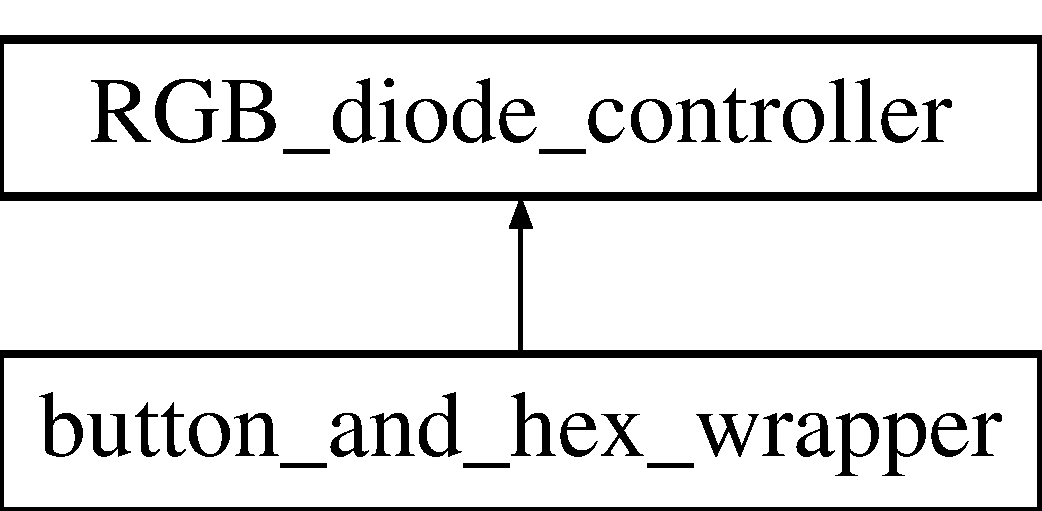
\includegraphics[height=2.000000cm]{classRGB__diode__controller}
\end{center}
\end{figure}
\subsection*{Entities}
\begin{DoxyCompactItemize}
\item 
\hyperlink{classRGB__diode__controller_1_1diode}{diode} architecture
\begin{DoxyCompactList}\small\item\em Architecture of the R\-G\-B\-\_\-diode. \end{DoxyCompactList}\end{DoxyCompactItemize}
\subsection*{Libraries}
 \begin{DoxyCompactItemize}
\item 
\hypertarget{classRGB__diode__controller_ae4f03c286607f3181e16b9aa12d0c6d4}{\hyperlink{classRGB__diode__controller_ae4f03c286607f3181e16b9aa12d0c6d4}{I\-E\-E\-E} }\label{classRGB__diode__controller_ae4f03c286607f3181e16b9aa12d0c6d4}

\begin{DoxyCompactList}\small\item\em Use of standard library. \end{DoxyCompactList}\end{DoxyCompactItemize}
\subsection*{Use Clauses}
 \begin{DoxyCompactItemize}
\item 
\hypertarget{classRGB__diode__controller_a68c233289eaf7d2601307bdd93b4c299}{\hyperlink{classRGB__diode__controller_a68c233289eaf7d2601307bdd93b4c299}{I\-E\-E\-E.\-S\-T\-D\-\_\-\-L\-O\-G\-I\-C\-\_\-1164.\-all}   }\label{classRGB__diode__controller_a68c233289eaf7d2601307bdd93b4c299}

\begin{DoxyCompactList}\small\item\em Use of standard logic arguments. \end{DoxyCompactList}\item 
\hypertarget{classRGB__diode__controller_a7c135c43c66ccd7f22abe5f6211788a5}{\hyperlink{classRGB__diode__controller_a7c135c43c66ccd7f22abe5f6211788a5}{I\-E\-E\-E.\-N\-U\-M\-E\-R\-I\-C\-\_\-\-S\-T\-D.\-all}   }\label{classRGB__diode__controller_a7c135c43c66ccd7f22abe5f6211788a5}

\begin{DoxyCompactList}\small\item\em Use of standard numerical arguments. \end{DoxyCompactList}\end{DoxyCompactItemize}
\subsection*{Generics}
 \begin{DoxyCompactItemize}
\item 
\hypertarget{classRGB__diode__controller_ad3971b999c08c97da803416025fcebb0}{\hyperlink{classRGB__diode__controller_ad3971b999c08c97da803416025fcebb0}{N} {\bfseries {\bfseries \textcolor{comment}{integer}\textcolor{vhdlchar}{ }\textcolor{vhdlchar}{\-:}\textcolor{vhdlchar}{=}\textcolor{vhdlchar}{ } \textcolor{vhdldigit}{1} \textcolor{vhdlchar}{ }}}}\label{classRGB__diode__controller_ad3971b999c08c97da803416025fcebb0}

\begin{DoxyCompactList}\small\item\em Generic to decide the duty cycle of the diode. Duty cycle = 1/(N+1) \end{DoxyCompactList}\end{DoxyCompactItemize}
\subsection*{Ports}
 \begin{DoxyCompactItemize}
\item 
\hypertarget{classRGB__diode__controller_a8120037e0ee47c35ba2d79242209c72e}{\hyperlink{classRGB__diode__controller_a8120037e0ee47c35ba2d79242209c72e}{clk}  {\bfseries {\bfseries \textcolor{vhdlkeyword}{in}\textcolor{vhdlchar}{ }}} {\bfseries \textcolor{comment}{S\-T\-D\-\_\-\-L\-O\-G\-I\-C}\textcolor{vhdlchar}{ }} }\label{classRGB__diode__controller_a8120037e0ee47c35ba2d79242209c72e}

\begin{DoxyCompactList}\small\item\em Clock in for calculation of duty cycle. \end{DoxyCompactList}\item 
\hypertarget{classRGB__diode__controller_aba021aec4b477b89079bb58ccadcc67e}{\hyperlink{classRGB__diode__controller_aba021aec4b477b89079bb58ccadcc67e}{rstn}  {\bfseries {\bfseries \textcolor{vhdlkeyword}{in}\textcolor{vhdlchar}{ }}} {\bfseries \textcolor{comment}{S\-T\-D\-\_\-\-L\-O\-G\-I\-C}\textcolor{vhdlchar}{ }} }\label{classRGB__diode__controller_aba021aec4b477b89079bb58ccadcc67e}

\begin{DoxyCompactList}\small\item\em Global reset, active low. \end{DoxyCompactList}\item 
\hypertarget{classRGB__diode__controller_a0ee3d978fb8b47588b62e4a768c780fe}{\hyperlink{classRGB__diode__controller_a0ee3d978fb8b47588b62e4a768c780fe}{diode\-\_\-out}  {\bfseries {\bfseries \textcolor{vhdlkeyword}{out}\textcolor{vhdlchar}{ }}} {\bfseries \textcolor{comment}{S\-T\-D\-\_\-\-L\-O\-G\-I\-C\-\_\-\-V\-E\-C\-T\-O\-R}\textcolor{vhdlchar}{ }\textcolor{vhdlchar}{(}\textcolor{vhdlchar}{ }\textcolor{vhdlchar}{ } \textcolor{vhdldigit}{2} \textcolor{vhdlchar}{ }\textcolor{vhdlchar}{ }\textcolor{vhdlchar}{ }\textcolor{vhdlkeyword}{downto}\textcolor{vhdlchar}{ }\textcolor{vhdlchar}{ }\textcolor{vhdlchar}{ } \textcolor{vhdldigit}{0} \textcolor{vhdlchar}{ }\textcolor{vhdlchar}{)}\textcolor{vhdlchar}{ }} }\label{classRGB__diode__controller_a0ee3d978fb8b47588b62e4a768c780fe}

\begin{DoxyCompactList}\small\item\em Diode\-\_\-out is a vector containing the state of the red, green and blue diode. \end{DoxyCompactList}\item 
\hypertarget{classRGB__diode__controller_a2027e6e92931979514fdb7cba1fa3b03}{\hyperlink{classRGB__diode__controller_a2027e6e92931979514fdb7cba1fa3b03}{is\-\_\-working}  {\bfseries {\bfseries \textcolor{vhdlkeyword}{in}\textcolor{vhdlchar}{ }}} {\bfseries \textcolor{comment}{S\-T\-D\-\_\-\-L\-O\-G\-I\-C}\textcolor{vhdlchar}{ }} }\label{classRGB__diode__controller_a2027e6e92931979514fdb7cba1fa3b03}

\begin{DoxyCompactList}\small\item\em Is\-\_\-working decides if the diode is to be green or red. \end{DoxyCompactList}\end{DoxyCompactItemize}


\subsection{Detailed Description}
The R\-G\-B\-\_\-control controls on of the onboard diodes. Depending on the input of the is\-\_\-working the diode will either be green or red. 

The documentation for this class was generated from the following file\-:\begin{DoxyCompactItemize}
\item 
\hyperlink{RGB__diode__controller_8vhd}{R\-G\-B\-\_\-diode\-\_\-controller.\-vhd}\end{DoxyCompactItemize}

\hypertarget{classseven__seg__control_1_1seven__crtl}{\section{seven\-\_\-crtl Architecture Reference}
\label{classseven__seg__control_1_1seven__crtl}\index{seven\-\_\-crtl@{seven\-\_\-crtl}}
}


Architecture of the \hyperlink{classseven__seg__control}{seven\-\_\-seg\-\_\-control}.  


\subsection*{Processes}
 \begin{DoxyCompactItemize}
\item 
\hypertarget{classseven__seg__control_1_1seven__crtl_a284632d205b54f8f9124b30aee6b1887}{\hyperlink{classseven__seg__control_1_1seven__crtl_a284632d205b54f8f9124b30aee6b1887}{P\-R\-O\-C\-E\-S\-S\-\_\-9}{\bfseries  ( {\bfseries {\bfseries \hyperlink{classseven__seg__control_aba021aec4b477b89079bb58ccadcc67e}{rstn}} \textcolor{vhdlchar}{ }\textcolor{vhdlchar}{ }\textcolor{vhdlchar}{ }} , {\bfseries {\bfseries \hyperlink{classseven__seg__control_a8120037e0ee47c35ba2d79242209c72e}{clk}} \textcolor{vhdlchar}{ }} )}}\label{classseven__seg__control_1_1seven__crtl_a284632d205b54f8f9124b30aee6b1887}

\end{DoxyCompactItemize}
\subsection*{Components}
 \begin{DoxyCompactItemize}
\item 
\hypertarget{classseven__seg__control_1_1seven__crtl_ac37f6407a40b9c2c6331c38048caf6f9}{\hyperlink{classseven__seg__control_1_1seven__crtl_ac37f6407a40b9c2c6331c38048caf6f9}{clk\-\_\-div\-\_\-seven\-\_\-seg}  {\bfseries }  }\label{classseven__seg__control_1_1seven__crtl_ac37f6407a40b9c2c6331c38048caf6f9}

\item 
\hypertarget{classseven__seg__control_1_1seven__crtl_aa2d5bf6e4dc6ef99dbc13d369781e56f}{\hyperlink{classseven__seg__control_1_1seven__crtl_aa2d5bf6e4dc6ef99dbc13d369781e56f}{bin2bcd}  {\bfseries }  }\label{classseven__seg__control_1_1seven__crtl_aa2d5bf6e4dc6ef99dbc13d369781e56f}

\end{DoxyCompactItemize}
\subsection*{Signals}
 \begin{DoxyCompactItemize}
\item 
\hypertarget{classseven__seg__control_1_1seven__crtl_a2b1cdd550105424013f7f1d5ecf590fd}{\hyperlink{classseven__seg__control_1_1seven__crtl_a2b1cdd550105424013f7f1d5ecf590fd}{cnt\-\_\-hex\-\_\-display} {\bfseries \textcolor{comment}{integer}\textcolor{vhdlchar}{ }\textcolor{vhdlkeyword}{range}\textcolor{vhdlchar}{ } \textcolor{vhdldigit}{0} \textcolor{vhdlchar}{ }\textcolor{vhdlchar}{ }\textcolor{vhdlchar}{ }\textcolor{vhdlkeyword}{to}\textcolor{vhdlchar}{ }\textcolor{vhdlchar}{ }\textcolor{vhdlchar}{ } \textcolor{vhdldigit}{7} \textcolor{vhdlchar}{ }} }\label{classseven__seg__control_1_1seven__crtl_a2b1cdd550105424013f7f1d5ecf590fd}

\begin{DoxyCompactList}\small\item\em A counter to decide what seven segment to be active. \end{DoxyCompactList}\item 
\hypertarget{classseven__seg__control_1_1seven__crtl_a5ba77dbe5578e704c37c2dde55e1033a}{\hyperlink{classseven__seg__control_1_1seven__crtl_a5ba77dbe5578e704c37c2dde55e1033a}{slow\-\_\-clk} {\bfseries \textcolor{comment}{S\-T\-D\-\_\-\-L\-O\-G\-I\-C}\textcolor{vhdlchar}{ }} }\label{classseven__seg__control_1_1seven__crtl_a5ba77dbe5578e704c37c2dde55e1033a}

\begin{DoxyCompactList}\small\item\em A clock for toggling between the seven segment displays. \end{DoxyCompactList}\item 
\hypertarget{classseven__seg__control_1_1seven__crtl_a5324433dce7401c1649a674673338373}{\hyperlink{classseven__seg__control_1_1seven__crtl_a5324433dce7401c1649a674673338373}{value\-\_\-vector} {\bfseries \textcolor{comment}{S\-T\-D\-\_\-\-L\-O\-G\-I\-C\-\_\-\-V\-E\-C\-T\-O\-R}\textcolor{vhdlchar}{ }\textcolor{vhdlchar}{(}\textcolor{vhdlchar}{ }\textcolor{vhdlchar}{ } \textcolor{vhdldigit}{31} \textcolor{vhdlchar}{ }\textcolor{vhdlchar}{ }\textcolor{vhdlchar}{ }\textcolor{vhdlkeyword}{downto}\textcolor{vhdlchar}{ }\textcolor{vhdlchar}{ }\textcolor{vhdlchar}{ } \textcolor{vhdldigit}{0} \textcolor{vhdlchar}{ }\textcolor{vhdlchar}{)}\textcolor{vhdlchar}{ }} }\label{classseven__seg__control_1_1seven__crtl_a5324433dce7401c1649a674673338373}

\begin{DoxyCompactList}\small\item\em This vector concatenates the current and selected value. \end{DoxyCompactList}\item 
\hypertarget{classseven__seg__control_1_1seven__crtl_ae3191418b7808fc159102056426355ad}{\hyperlink{classseven__seg__control_1_1seven__crtl_ae3191418b7808fc159102056426355ad}{current\-\_\-number} {\bfseries \textcolor{comment}{integer}\textcolor{vhdlchar}{ }\textcolor{vhdlkeyword}{range}\textcolor{vhdlchar}{ } \textcolor{vhdldigit}{0} \textcolor{vhdlchar}{ }\textcolor{vhdlchar}{ }\textcolor{vhdlchar}{ }\textcolor{vhdlkeyword}{to}\textcolor{vhdlchar}{ }\textcolor{vhdlchar}{ }\textcolor{vhdlchar}{ } \textcolor{vhdldigit}{9} \textcolor{vhdlchar}{ }} }\label{classseven__seg__control_1_1seven__crtl_ae3191418b7808fc159102056426355ad}

\begin{DoxyCompactList}\small\item\em This signal indicated the current number to be outputted on the seven segment selected. \end{DoxyCompactList}\end{DoxyCompactItemize}
\subsection*{Instantiations}
 \begin{DoxyCompactItemize}
\item 
\hypertarget{classseven__seg__control_1_1seven__crtl_a4f65bad50a70c230d8cab7826ca467b3}{\hyperlink{classseven__seg__control_1_1seven__crtl_a4f65bad50a70c230d8cab7826ca467b3}{bin\-\_\-2\-\_\-bcd\-\_\-inst\-\_\-current}  {\bfseries bin2bcd}   }\label{classseven__seg__control_1_1seven__crtl_a4f65bad50a70c230d8cab7826ca467b3}

\item 
\hypertarget{classseven__seg__control_1_1seven__crtl_a175226958b1074f166ae2f0324937b3b}{\hyperlink{classseven__seg__control_1_1seven__crtl_a175226958b1074f166ae2f0324937b3b}{bin\-\_\-2\-\_\-bcd\-\_\-inst\-\_\-selected}  {\bfseries bin2bcd}   }\label{classseven__seg__control_1_1seven__crtl_a175226958b1074f166ae2f0324937b3b}

\item 
\hypertarget{classseven__seg__control_1_1seven__crtl_a39b27375c53f9cfc5759f4a53877ba0b}{\hyperlink{classseven__seg__control_1_1seven__crtl_a39b27375c53f9cfc5759f4a53877ba0b}{clk\-\_\-div}  {\bfseries clk\-\_\-div\-\_\-seven\-\_\-seg}   }\label{classseven__seg__control_1_1seven__crtl_a39b27375c53f9cfc5759f4a53877ba0b}

\end{DoxyCompactItemize}


\subsection{Detailed Description}
Architecture of the \hyperlink{classseven__seg__control}{seven\-\_\-seg\-\_\-control}. 

The \hyperlink{classseven__seg__control}{seven\-\_\-seg\-\_\-control} controls the output of the seven segment displays. To do this the modules uses \hyperlink{classclk__div__seven__seg}{clk\-\_\-div\-\_\-seven\-\_\-seg} to divide the clock to a suitable speed to the seven\-\_\-seg\-\_\-sel to switch. This module also uses \hyperlink{classbin2bcd}{bin2bcd} to convert the numbers from binary to B\-C\-D. The B\-C\-D is then converted to seven segment numbers and outputted on the seven\-\_\-seg\-\_\-out. 

The documentation for this class was generated from the following files\-:\begin{DoxyCompactItemize}
\item 
\hyperlink{seven__seg__control_8vhd}{seven\-\_\-seg\-\_\-control.\-vhd}\end{DoxyCompactItemize}

\hypertarget{classseven__seg__control}{\section{seven\-\_\-seg\-\_\-control Entity Reference}
\label{classseven__seg__control}\index{seven\-\_\-seg\-\_\-control@{seven\-\_\-seg\-\_\-control}}
}


The seven segment dispay takes two 8 bit integers in and outputs these on an 8 digit seven segment display.  


Inheritance diagram for seven\-\_\-seg\-\_\-control\-:\begin{figure}[H]
\begin{center}
\leavevmode
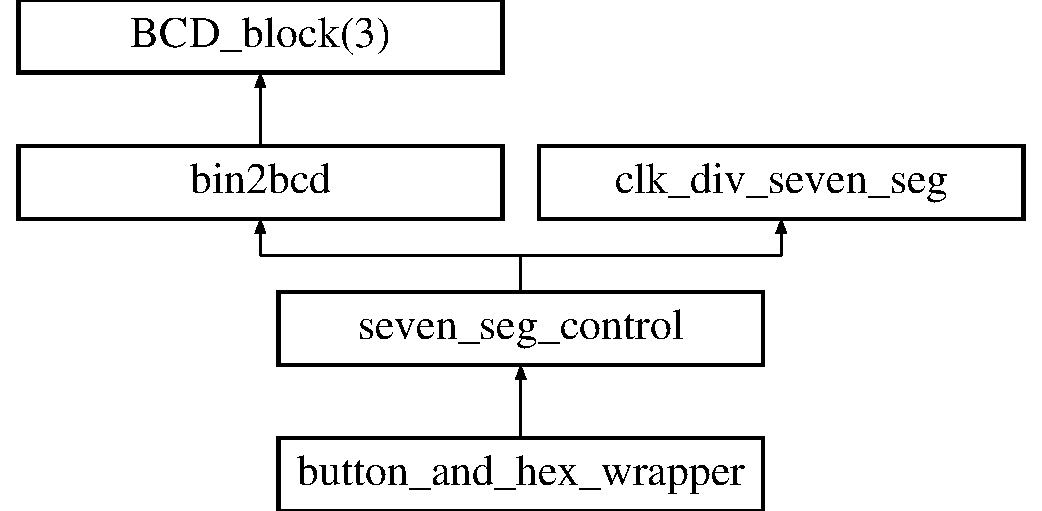
\includegraphics[height=4.000000cm]{classseven__seg__control}
\end{center}
\end{figure}
\subsection*{Entities}
\begin{DoxyCompactItemize}
\item 
\hyperlink{classseven__seg__control_1_1RTL}{R\-T\-L} architecture
\begin{DoxyCompactList}\small\item\em Architecture of the \hyperlink{classseven__seg__control}{seven\-\_\-seg\-\_\-control}. \end{DoxyCompactList}\end{DoxyCompactItemize}
\subsection*{Libraries}
 \begin{DoxyCompactItemize}
\item 
\hypertarget{classseven__seg__control_ae4f03c286607f3181e16b9aa12d0c6d4}{\hyperlink{classseven__seg__control_ae4f03c286607f3181e16b9aa12d0c6d4}{I\-E\-E\-E} }\label{classseven__seg__control_ae4f03c286607f3181e16b9aa12d0c6d4}

\begin{DoxyCompactList}\small\item\em Use of standard library. \end{DoxyCompactList}\end{DoxyCompactItemize}
\subsection*{Use Clauses}
 \begin{DoxyCompactItemize}
\item 
\hypertarget{classseven__seg__control_a68c233289eaf7d2601307bdd93b4c299}{\hyperlink{classseven__seg__control_a68c233289eaf7d2601307bdd93b4c299}{I\-E\-E\-E.\-S\-T\-D\-\_\-\-L\-O\-G\-I\-C\-\_\-1164.\-all}   }\label{classseven__seg__control_a68c233289eaf7d2601307bdd93b4c299}

\begin{DoxyCompactList}\small\item\em Use of standard logic arguments. \end{DoxyCompactList}\item 
\hypertarget{classseven__seg__control_a7c135c43c66ccd7f22abe5f6211788a5}{\hyperlink{classseven__seg__control_a7c135c43c66ccd7f22abe5f6211788a5}{I\-E\-E\-E.\-N\-U\-M\-E\-R\-I\-C\-\_\-\-S\-T\-D.\-all}   }\label{classseven__seg__control_a7c135c43c66ccd7f22abe5f6211788a5}

\begin{DoxyCompactList}\small\item\em Use of standard numerical arguments. \end{DoxyCompactList}\end{DoxyCompactItemize}
\subsection*{Ports}
 \begin{DoxyCompactItemize}
\item 
\hypertarget{classseven__seg__control_a8120037e0ee47c35ba2d79242209c72e}{\hyperlink{classseven__seg__control_a8120037e0ee47c35ba2d79242209c72e}{clk}  {\bfseries {\bfseries \textcolor{vhdlkeyword}{in}\textcolor{vhdlchar}{ }}} {\bfseries \textcolor{comment}{S\-T\-D\-\_\-\-L\-O\-G\-I\-C}\textcolor{vhdlchar}{ }} }\label{classseven__seg__control_a8120037e0ee47c35ba2d79242209c72e}

\begin{DoxyCompactList}\small\item\em Input clock for registers and the clock divider. \end{DoxyCompactList}\item 
\hypertarget{classseven__seg__control_aba021aec4b477b89079bb58ccadcc67e}{\hyperlink{classseven__seg__control_aba021aec4b477b89079bb58ccadcc67e}{rstn}  {\bfseries {\bfseries \textcolor{vhdlkeyword}{in}\textcolor{vhdlchar}{ }}} {\bfseries \textcolor{comment}{S\-T\-D\-\_\-\-L\-O\-G\-I\-C}\textcolor{vhdlchar}{ }} }\label{classseven__seg__control_aba021aec4b477b89079bb58ccadcc67e}

\begin{DoxyCompactList}\small\item\em Global reset, active low. \end{DoxyCompactList}\item 
\hypertarget{classseven__seg__control_abdc5a927ef7ee61296cb6236260e149a}{\hyperlink{classseven__seg__control_abdc5a927ef7ee61296cb6236260e149a}{current\-\_\-preset}  {\bfseries {\bfseries \textcolor{vhdlkeyword}{in}\textcolor{vhdlchar}{ }}} {\bfseries \textcolor{comment}{S\-T\-D\-\_\-\-L\-O\-G\-I\-C\-\_\-\-V\-E\-C\-T\-O\-R}\textcolor{vhdlchar}{ }\textcolor{vhdlchar}{(}\textcolor{vhdlchar}{ }\textcolor{vhdlchar}{ } \textcolor{vhdldigit}{7} \textcolor{vhdlchar}{ }\textcolor{vhdlchar}{ }\textcolor{vhdlchar}{ }\textcolor{vhdlkeyword}{downto}\textcolor{vhdlchar}{ }\textcolor{vhdlchar}{ }\textcolor{vhdlchar}{ } \textcolor{vhdldigit}{0} \textcolor{vhdlchar}{ }\textcolor{vhdlchar}{)}\textcolor{vhdlchar}{ }} }\label{classseven__seg__control_abdc5a927ef7ee61296cb6236260e149a}

\begin{DoxyCompactList}\small\item\em Current\-\_\-preset marks the preset to be selected. \end{DoxyCompactList}\item 
\hypertarget{classseven__seg__control_a4b2e584fda5f9b503d3f23e9bd793c33}{\hyperlink{classseven__seg__control_a4b2e584fda5f9b503d3f23e9bd793c33}{selected\-\_\-preset}  {\bfseries {\bfseries \textcolor{vhdlkeyword}{in}\textcolor{vhdlchar}{ }}} {\bfseries \textcolor{comment}{S\-T\-D\-\_\-\-L\-O\-G\-I\-C\-\_\-\-V\-E\-C\-T\-O\-R}\textcolor{vhdlchar}{ }\textcolor{vhdlchar}{(}\textcolor{vhdlchar}{ }\textcolor{vhdlchar}{ } \textcolor{vhdldigit}{7} \textcolor{vhdlchar}{ }\textcolor{vhdlchar}{ }\textcolor{vhdlchar}{ }\textcolor{vhdlkeyword}{downto}\textcolor{vhdlchar}{ }\textcolor{vhdlchar}{ }\textcolor{vhdlchar}{ } \textcolor{vhdldigit}{0} \textcolor{vhdlchar}{ }\textcolor{vhdlchar}{)}\textcolor{vhdlchar}{ }} }\label{classseven__seg__control_a4b2e584fda5f9b503d3f23e9bd793c33}

\begin{DoxyCompactList}\small\item\em Selected\-\_\-preset marks the current selected preset. \end{DoxyCompactList}\item 
\hypertarget{classseven__seg__control_a45655c10fcad02d37d83f5279ebb199b}{\hyperlink{classseven__seg__control_a45655c10fcad02d37d83f5279ebb199b}{seven\-\_\-seg\-\_\-out}  {\bfseries {\bfseries \textcolor{vhdlkeyword}{out}\textcolor{vhdlchar}{ }}} {\bfseries \textcolor{comment}{S\-T\-D\-\_\-\-L\-O\-G\-I\-C\-\_\-\-V\-E\-C\-T\-O\-R}\textcolor{vhdlchar}{ }\textcolor{vhdlchar}{(}\textcolor{vhdlchar}{ }\textcolor{vhdlchar}{ } \textcolor{vhdldigit}{6} \textcolor{vhdlchar}{ }\textcolor{vhdlchar}{ }\textcolor{vhdlchar}{ }\textcolor{vhdlkeyword}{downto}\textcolor{vhdlchar}{ }\textcolor{vhdlchar}{ }\textcolor{vhdlchar}{ } \textcolor{vhdldigit}{0} \textcolor{vhdlchar}{ }\textcolor{vhdlchar}{)}\textcolor{vhdlchar}{ }} }\label{classseven__seg__control_a45655c10fcad02d37d83f5279ebb199b}

\begin{DoxyCompactList}\small\item\em Seven\-\_\-sel\-\_\-out marks the seven segment display of the current selected seven segment display segment. \end{DoxyCompactList}\item 
\hypertarget{classseven__seg__control_ae1646bd2ce2b0e1d1bb85bf2a88d1b5f}{\hyperlink{classseven__seg__control_ae1646bd2ce2b0e1d1bb85bf2a88d1b5f}{seven\-\_\-seg\-\_\-sel}  {\bfseries {\bfseries \textcolor{vhdlkeyword}{out}\textcolor{vhdlchar}{ }}} {\bfseries \textcolor{comment}{S\-T\-D\-\_\-\-L\-O\-G\-I\-C\-\_\-\-V\-E\-C\-T\-O\-R}\textcolor{vhdlchar}{ }\textcolor{vhdlchar}{(}\textcolor{vhdlchar}{ }\textcolor{vhdlchar}{ } \textcolor{vhdldigit}{7} \textcolor{vhdlchar}{ }\textcolor{vhdlchar}{ }\textcolor{vhdlchar}{ }\textcolor{vhdlkeyword}{downto}\textcolor{vhdlchar}{ }\textcolor{vhdlchar}{ }\textcolor{vhdlchar}{ } \textcolor{vhdldigit}{0} \textcolor{vhdlchar}{ }\textcolor{vhdlchar}{)}\textcolor{vhdlchar}{ }} }\label{classseven__seg__control_ae1646bd2ce2b0e1d1bb85bf2a88d1b5f}

\begin{DoxyCompactList}\small\item\em Seven\-\_\-seg\-\_\-sel marks the current selected seven segment display. \end{DoxyCompactList}\end{DoxyCompactItemize}


\subsection{Detailed Description}
The seven segment dispay takes two 8 bit integers in and outputs these on an 8 digit seven segment display. 

The documentation for this class was generated from the following file\-:\begin{DoxyCompactItemize}
\item 
\hyperlink{seven__seg__control_8vhd}{seven\-\_\-seg\-\_\-control.\-vhd}\end{DoxyCompactItemize}

\hypertarget{classDAC__SPI_1_1SPI}{\section{S\-P\-I Architecture Reference}
\label{classDAC__SPI_1_1SPI}\index{S\-P\-I@{S\-P\-I}}
}


Architecture of the \hyperlink{classDAC__SPI}{D\-A\-C\-\_\-\-S\-P\-I}.  


\subsection*{Processes}
 \begin{DoxyCompactItemize}
\item 
\hypertarget{classDAC__SPI_1_1SPI_a242d986315a0356a0eab33f27aaf9ee0}{\hyperlink{classDAC__SPI_1_1SPI_a242d986315a0356a0eab33f27aaf9ee0}{data\-Out}{\bfseries  ( {\bfseries {\bfseries \hyperlink{classDAC__SPI_aba021aec4b477b89079bb58ccadcc67e}{rstn}} \textcolor{vhdlchar}{ }\textcolor{vhdlchar}{ }\textcolor{vhdlchar}{ }} , {\bfseries {\bfseries \hyperlink{classDAC__SPI_a8120037e0ee47c35ba2d79242209c72e}{clk}} \textcolor{vhdlchar}{ }} )}}\label{classDAC__SPI_1_1SPI_a242d986315a0356a0eab33f27aaf9ee0}

\end{DoxyCompactItemize}
\subsection*{Signals}
 \begin{DoxyCompactItemize}
\item 
\hypertarget{classDAC__SPI_1_1SPI_a59fba5ee7156ef44b2afe3d3d4d71a85}{\hyperlink{classDAC__SPI_1_1SPI_a59fba5ee7156ef44b2afe3d3d4d71a85}{data\-Counter} {\bfseries \textcolor{comment}{integer}\textcolor{vhdlchar}{ }\textcolor{vhdlkeyword}{range}\textcolor{vhdlchar}{ } \textcolor{vhdldigit}{0} \textcolor{vhdlchar}{ }\textcolor{vhdlchar}{ }\textcolor{vhdlchar}{ }\textcolor{vhdlkeyword}{to}\textcolor{vhdlchar}{ }\textcolor{vhdlchar}{ }\textcolor{vhdlchar}{ } \textcolor{vhdldigit}{25} \textcolor{vhdlchar}{ }} }\label{classDAC__SPI_1_1SPI_a59fba5ee7156ef44b2afe3d3d4d71a85}

\begin{DoxyCompactList}\small\item\em This signal keeps track on what bit to send over the \hyperlink{classDAC__SPI_1_1SPI}{S\-P\-I}. \end{DoxyCompactList}\item 
\hypertarget{classDAC__SPI_1_1SPI_aa1fedcfa30798eabcce4a1b1cdd6fa7a}{\hyperlink{classDAC__SPI_1_1SPI_aa1fedcfa30798eabcce4a1b1cdd6fa7a}{config\-Bits} {\bfseries \textcolor{comment}{S\-T\-D\-\_\-\-L\-O\-G\-I\-C\-\_\-\-V\-E\-C\-T\-O\-R}\textcolor{vhdlchar}{ }\textcolor{vhdlchar}{(}\textcolor{vhdlchar}{ }\textcolor{vhdlchar}{ } \textcolor{vhdldigit}{7} \textcolor{vhdlchar}{ }\textcolor{vhdlchar}{ }\textcolor{vhdlchar}{ }\textcolor{vhdlkeyword}{downto}\textcolor{vhdlchar}{ }\textcolor{vhdlchar}{ }\textcolor{vhdlchar}{ } \textcolor{vhdldigit}{0} \textcolor{vhdlchar}{ }\textcolor{vhdlchar}{)}\textcolor{vhdlchar}{ }} }\label{classDAC__SPI_1_1SPI_aa1fedcfa30798eabcce4a1b1cdd6fa7a}

\begin{DoxyCompactList}\small\item\em Bits containing configuration information for the D\-A\-C. \end{DoxyCompactList}\item 
\hypertarget{classDAC__SPI_1_1SPI_afda8ab14219d5cf291d97fd808265f14}{\hyperlink{classDAC__SPI_1_1SPI_afda8ab14219d5cf291d97fd808265f14}{lastsampleclk} {\bfseries \textcolor{comment}{S\-T\-D\-\_\-\-L\-O\-G\-I\-C}\textcolor{vhdlchar}{ }} }\label{classDAC__SPI_1_1SPI_afda8ab14219d5cf291d97fd808265f14}

\begin{DoxyCompactList}\small\item\em Bit storing the last value of the sampleclk. \end{DoxyCompactList}\item 
\hypertarget{classDAC__SPI_1_1SPI_a3ba18b13dd42cfbe57a176e0793f0e15}{\hyperlink{classDAC__SPI_1_1SPI_a3ba18b13dd42cfbe57a176e0793f0e15}{databuff} {\bfseries \textcolor{comment}{S\-T\-D\-\_\-\-L\-O\-G\-I\-C\-\_\-vector}\textcolor{vhdlchar}{ }\textcolor{vhdlchar}{(}\textcolor{vhdlchar}{ }\textcolor{vhdlchar}{ } \textcolor{vhdldigit}{15} \textcolor{vhdlchar}{ }\textcolor{vhdlchar}{ }\textcolor{vhdlchar}{ }\textcolor{vhdlkeyword}{downto}\textcolor{vhdlchar}{ }\textcolor{vhdlchar}{ }\textcolor{vhdlchar}{ } \textcolor{vhdldigit}{0} \textcolor{vhdlchar}{ }\textcolor{vhdlchar}{)}\textcolor{vhdlchar}{ }} }\label{classDAC__SPI_1_1SPI_a3ba18b13dd42cfbe57a176e0793f0e15}

\begin{DoxyCompactList}\small\item\em Bit sampling the input data to make sure it is not changed during transmission. \end{DoxyCompactList}\end{DoxyCompactItemize}


\subsection{Detailed Description}
Architecture of the \hyperlink{classDAC__SPI}{D\-A\-C\-\_\-\-S\-P\-I}. 

The architecture containing the main body of the component. 

The documentation for this class was generated from the following file\-:\begin{DoxyCompactItemize}
\item 
\hyperlink{DAC__SPI_8vhd}{D\-A\-C\-\_\-\-S\-P\-I.\-vhd}\end{DoxyCompactItemize}

\hypertarget{classADC__TOP_1_1TOP__ADC}{\section{T\-O\-P\-\_\-\-A\-D\-C Architecture Reference}
\label{classADC__TOP_1_1TOP__ADC}\index{T\-O\-P\-\_\-\-A\-D\-C@{T\-O\-P\-\_\-\-A\-D\-C}}
}


\hyperlink{classADC__TOP}{A\-D\-C\-\_\-\-T\-O\-P}.  


\subsection*{Processes}
 \begin{DoxyCompactItemize}
\item 
\hypertarget{classADC__TOP_1_1TOP__ADC_af7530dff761625dab17b84e8c5926692}{\hyperlink{classADC__TOP_1_1TOP__ADC_af7530dff761625dab17b84e8c5926692}{P\-R\-O\-C\-E\-S\-S\-\_\-1}{\bfseries  ( {\bfseries {\bfseries \hyperlink{classADC__TOP_ab1f7becce7cb29d94bb2f2ec187f72a4}{C\-L\-K100}} \textcolor{vhdlchar}{ }\textcolor{vhdlchar}{ }\textcolor{vhdlchar}{ }} , {\bfseries {\bfseries \hyperlink{classADC__TOP_a91cf794d165cc0a740042335a6062940}{R\-S\-T}} \textcolor{vhdlchar}{ }} )}}\label{classADC__TOP_1_1TOP__ADC_af7530dff761625dab17b84e8c5926692}

\end{DoxyCompactItemize}
\subsection*{Components}
 \begin{DoxyCompactItemize}
\item 
\hypertarget{classADC__TOP_1_1TOP__ADC_ae43da35f6da7738b69d6245cc2ca3b49}{\hyperlink{classADC__TOP_1_1TOP__ADC_ae43da35f6da7738b69d6245cc2ca3b49}{digitalfilter}  {\bfseries }  }\label{classADC__TOP_1_1TOP__ADC_ae43da35f6da7738b69d6245cc2ca3b49}

\begin{DoxyCompactList}\small\item\em Digital F\-I\-R filter. \end{DoxyCompactList}\item 
\hypertarget{classADC__TOP_1_1TOP__ADC_ad251174263b28388454816799ffd91ae}{\hyperlink{classADC__TOP_1_1TOP__ADC_ad251174263b28388454816799ffd91ae}{A\-D\-C}  {\bfseries }  }\label{classADC__TOP_1_1TOP__ADC_ad251174263b28388454816799ffd91ae}

\begin{DoxyCompactList}\small\item\em finished indicates the filter calculations are done \end{DoxyCompactList}\item 
\hypertarget{classADC__TOP_1_1TOP__ADC_a76d32257e982d92a96905d3f9b3babc8}{\hyperlink{classADC__TOP_1_1TOP__ADC_a76d32257e982d92a96905d3f9b3babc8}{A\-D\-C\-\_\-buffer}  {\bfseries }  }\label{classADC__TOP_1_1TOP__ADC_a76d32257e982d92a96905d3f9b3babc8}

\begin{DoxyCompactList}\small\item\em Buffer for samples. \end{DoxyCompactList}\end{DoxyCompactItemize}
\subsection*{Signals}
 \begin{DoxyCompactItemize}
\item 
\hypertarget{classADC__TOP_1_1TOP__ADC_ab48f33ef761b1b52e2b08c1d8ef76334}{\hyperlink{classADC__TOP_1_1TOP__ADC_ab48f33ef761b1b52e2b08c1d8ef76334}{den\-\_\-in} {\bfseries \textcolor{comment}{S\-T\-D\-\_\-\-L\-O\-G\-I\-C}\textcolor{vhdlchar}{ }} }\label{classADC__TOP_1_1TOP__ADC_ab48f33ef761b1b52e2b08c1d8ef76334}

\begin{DoxyCompactList}\small\item\em Address indicates what address bufferout should be read from Signal for den\-\_\-in in the X\-A\-D\-C. \end{DoxyCompactList}\item 
\hypertarget{classADC__TOP_1_1TOP__ADC_afeaa67943e27d8c3ee9651159bd9193d}{\hyperlink{classADC__TOP_1_1TOP__ADC_afeaa67943e27d8c3ee9651159bd9193d}{dwe\-\_\-in} {\bfseries \textcolor{comment}{std\-\_\-logic}\textcolor{vhdlchar}{ }} }\label{classADC__TOP_1_1TOP__ADC_afeaa67943e27d8c3ee9651159bd9193d}

\begin{DoxyCompactList}\small\item\em Signal for the write enable in for the X\-A\-D\-C. \end{DoxyCompactList}\item 
\hypertarget{classADC__TOP_1_1TOP__ADC_a6116bc00f8788e5cc6bc5deb069fdc53}{\hyperlink{classADC__TOP_1_1TOP__ADC_a6116bc00f8788e5cc6bc5deb069fdc53}{di\-\_\-in} {\bfseries \textcolor{comment}{S\-T\-D\-\_\-\-L\-O\-G\-I\-C\-\_\-\-V\-E\-C\-T\-O\-R}\textcolor{vhdlchar}{ }\textcolor{vhdlchar}{(}\textcolor{vhdlchar}{ }\textcolor{vhdlchar}{ } \textcolor{vhdldigit}{15} \textcolor{vhdlchar}{ }\textcolor{vhdlchar}{ }\textcolor{vhdlchar}{ }\textcolor{vhdlkeyword}{downto}\textcolor{vhdlchar}{ }\textcolor{vhdlchar}{ }\textcolor{vhdlchar}{ } \textcolor{vhdldigit}{0} \textcolor{vhdlchar}{ }\textcolor{vhdlchar}{)}\textcolor{vhdlchar}{ }} }\label{classADC__TOP_1_1TOP__ADC_a6116bc00f8788e5cc6bc5deb069fdc53}

\begin{DoxyCompactList}\small\item\em Signal for the input vector for the X\-A\-D\-C. \end{DoxyCompactList}\item 
\hypertarget{classADC__TOP_1_1TOP__ADC_a72126e522b97fa2b659a65d687081a41}{\hyperlink{classADC__TOP_1_1TOP__ADC_a72126e522b97fa2b659a65d687081a41}{daddr\-\_\-in} {\bfseries \textcolor{comment}{std\-\_\-\-L\-O\-G\-I\-C\-\_\-vector}\textcolor{vhdlchar}{ }\textcolor{vhdlchar}{(}\textcolor{vhdlchar}{ }\textcolor{vhdlchar}{ } \textcolor{vhdldigit}{6} \textcolor{vhdlchar}{ }\textcolor{vhdlchar}{ }\textcolor{vhdlchar}{ }\textcolor{vhdlkeyword}{downto}\textcolor{vhdlchar}{ }\textcolor{vhdlchar}{ }\textcolor{vhdlchar}{ } \textcolor{vhdldigit}{0} \textcolor{vhdlchar}{ }\textcolor{vhdlchar}{)}\textcolor{vhdlchar}{ }} }\label{classADC__TOP_1_1TOP__ADC_a72126e522b97fa2b659a65d687081a41}

\begin{DoxyCompactList}\small\item\em Address in registers. \end{DoxyCompactList}\item 
\hypertarget{classADC__TOP_1_1TOP__ADC_ac58565a65b10392b2476534d234c8871}{\hyperlink{classADC__TOP_1_1TOP__ADC_ac58565a65b10392b2476534d234c8871}{inv\-\_\-rst} {\bfseries \textcolor{comment}{std\-\_\-logic}\textcolor{vhdlchar}{ }} }\label{classADC__TOP_1_1TOP__ADC_ac58565a65b10392b2476534d234c8871}

\begin{DoxyCompactList}\small\item\em Inversed reset for X\-A\-D\-C. \end{DoxyCompactList}\item 
\hypertarget{classADC__TOP_1_1TOP__ADC_ad5797d4ae2d654477e555700f8c3e43f}{\hyperlink{classADC__TOP_1_1TOP__ADC_ad5797d4ae2d654477e555700f8c3e43f}{sampledvalue} {\bfseries \textcolor{comment}{S\-T\-D\-\_\-\-L\-O\-G\-I\-C\-\_\-\-V\-E\-C\-T\-O\-R}\textcolor{vhdlchar}{ }\textcolor{vhdlchar}{(}\textcolor{vhdlchar}{ }\textcolor{vhdlchar}{ } \textcolor{vhdldigit}{15} \textcolor{vhdlchar}{ }\textcolor{vhdlchar}{ }\textcolor{vhdlchar}{ }\textcolor{vhdlkeyword}{downto}\textcolor{vhdlchar}{ }\textcolor{vhdlchar}{ }\textcolor{vhdlchar}{ } \textcolor{vhdldigit}{0} \textcolor{vhdlchar}{ }\textcolor{vhdlchar}{)}\textcolor{vhdlchar}{ }} }\label{classADC__TOP_1_1TOP__ADC_ad5797d4ae2d654477e555700f8c3e43f}

\begin{DoxyCompactList}\small\item\em Sampled value from X\-A\-D\-C. \end{DoxyCompactList}\item 
\hypertarget{classADC__TOP_1_1TOP__ADC_a765e6fd5e52807fd480f8e8477f35144}{\hyperlink{classADC__TOP_1_1TOP__ADC_a765e6fd5e52807fd480f8e8477f35144}{busy} {\bfseries \textcolor{comment}{S\-T\-D\-\_\-\-L\-O\-G\-I\-C}\textcolor{vhdlchar}{ }} }\label{classADC__TOP_1_1TOP__ADC_a765e6fd5e52807fd480f8e8477f35144}

\begin{DoxyCompactList}\small\item\em Busy signal from X\-A\-D\-C. \end{DoxyCompactList}\item 
\hypertarget{classADC__TOP_1_1TOP__ADC_afda8ab14219d5cf291d97fd808265f14}{\hyperlink{classADC__TOP_1_1TOP__ADC_afda8ab14219d5cf291d97fd808265f14}{lastsampleclk} {\bfseries \textcolor{comment}{S\-T\-D\-\_\-\-L\-O\-G\-I\-C}\textcolor{vhdlchar}{ }} }\label{classADC__TOP_1_1TOP__ADC_afda8ab14219d5cf291d97fd808265f14}

\begin{DoxyCompactList}\small\item\em The sample clock delayed one C\-L\-K. \end{DoxyCompactList}\item 
\hypertarget{classADC__TOP_1_1TOP__ADC_ac455bd1063158947568362bdce5e54c2}{\hyperlink{classADC__TOP_1_1TOP__ADC_ac455bd1063158947568362bdce5e54c2}{filterin} {\bfseries \textcolor{comment}{S\-T\-D\-\_\-\-L\-O\-G\-I\-C\-\_\-\-V\-E\-C\-T\-O\-R}\textcolor{vhdlchar}{ }\textcolor{vhdlchar}{(}\textcolor{vhdlchar}{ }\textcolor{vhdlchar}{ } \textcolor{vhdldigit}{31} \textcolor{vhdlchar}{ }\textcolor{vhdlchar}{ }\textcolor{vhdlchar}{ }\textcolor{vhdlkeyword}{downto}\textcolor{vhdlchar}{ }\textcolor{vhdlchar}{ }\textcolor{vhdlchar}{ } \textcolor{vhdldigit}{0} \textcolor{vhdlchar}{ }\textcolor{vhdlchar}{)}\textcolor{vhdlchar}{ }} }\label{classADC__TOP_1_1TOP__ADC_ac455bd1063158947568362bdce5e54c2}

\begin{DoxyCompactList}\small\item\em The sampled value extended to 32 bits as input to the digital filter. \end{DoxyCompactList}\item 
\hypertarget{classADC__TOP_1_1TOP__ADC_ac6146f465208802b4d06d2f701308cf4}{\hyperlink{classADC__TOP_1_1TOP__ADC_ac6146f465208802b4d06d2f701308cf4}{filterout} {\bfseries \textcolor{comment}{S\-T\-D\-\_\-\-L\-O\-G\-I\-C\-\_\-\-V\-E\-C\-T\-O\-R}\textcolor{vhdlchar}{ }\textcolor{vhdlchar}{(}\textcolor{vhdlchar}{ }\textcolor{vhdlchar}{ } \textcolor{vhdldigit}{31} \textcolor{vhdlchar}{ }\textcolor{vhdlchar}{ }\textcolor{vhdlchar}{ }\textcolor{vhdlkeyword}{downto}\textcolor{vhdlchar}{ }\textcolor{vhdlchar}{ }\textcolor{vhdlchar}{ } \textcolor{vhdldigit}{0} \textcolor{vhdlchar}{ }\textcolor{vhdlchar}{)}\textcolor{vhdlchar}{ }} }\label{classADC__TOP_1_1TOP__ADC_ac6146f465208802b4d06d2f701308cf4}

\begin{DoxyCompactList}\small\item\em The output of the digital filter and input of the buffer. \end{DoxyCompactList}\end{DoxyCompactItemize}
\subsection*{Attributes}
 \begin{DoxyCompactItemize}
\item 
\hypertarget{classADC__TOP_1_1TOP__ADC_a32f4997bcfad751ba77794903af40d92}{\hyperlink{classADC__TOP_1_1TOP__ADC_a32f4997bcfad751ba77794903af40d92}{S\-Y\-N\-\_\-\-B\-L\-A\-C\-K\-\_\-\-B\-O\-X\-\_\-\-A\-D\-C} {\bfseries \textcolor{comment}{B\-O\-O\-L\-E\-A\-N}\textcolor{vhdlchar}{ }} }\label{classADC__TOP_1_1TOP__ADC_a32f4997bcfad751ba77794903af40d92}

\begin{DoxyCompactList}\small\item\em Signaling the A\-D\-C is busy sampling. \end{DoxyCompactList}\item 
\hypertarget{classADC__TOP_1_1TOP__ADC_a737609c62913b04be3bb776fbce18464}{\hyperlink{classADC__TOP_1_1TOP__ADC_a737609c62913b04be3bb776fbce18464}{S\-Y\-N\-\_\-\-B\-L\-A\-C\-K\-\_\-\-B\-O\-X\-\_\-\-A\-D\-C} {\bfseries {\bfseries \hyperlink{classADC__TOP_1_1TOP__ADC_ad251174263b28388454816799ffd91ae}{A\-D\-C}} \textcolor{vhdlchar}{ }\textcolor{vhdlchar}{\-:}\textcolor{vhdlchar}{ }\textcolor{vhdlkeyword}{component}\textcolor{vhdlchar}{ }\textcolor{vhdlkeyword}{is}\textcolor{vhdlchar}{ }\textcolor{vhdlchar}{T\-R\-U\-E}\textcolor{vhdlchar}{ }} }\label{classADC__TOP_1_1TOP__ADC_a737609c62913b04be3bb776fbce18464}

\item 
\hypertarget{classADC__TOP_1_1TOP__ADC_a05f1935151676cf5c0d14df52f28c3b1}{\hyperlink{classADC__TOP_1_1TOP__ADC_a05f1935151676cf5c0d14df52f28c3b1}{B\-L\-A\-C\-K\-\_\-\-B\-O\-X\-\_\-\-P\-A\-D\-\_\-\-P\-I\-N\-\_\-\-A\-D\-C} {\bfseries \textcolor{comment}{S\-T\-R\-I\-N\-G}\textcolor{vhdlchar}{ }} }\label{classADC__TOP_1_1TOP__ADC_a05f1935151676cf5c0d14df52f28c3b1}

\item 
\hypertarget{classADC__TOP_1_1TOP__ADC_a731a305d96f244bae6982ef51e5298be}{\hyperlink{classADC__TOP_1_1TOP__ADC_a731a305d96f244bae6982ef51e5298be}{B\-L\-A\-C\-K\-\_\-\-B\-O\-X\-\_\-\-P\-A\-D\-\_\-\-P\-I\-N\-\_\-\-A\-D\-C} {\bfseries {\bfseries \hyperlink{classADC__TOP_1_1TOP__ADC_ad251174263b28388454816799ffd91ae}{A\-D\-C}} \textcolor{vhdlchar}{ }\textcolor{vhdlchar}{\-:}\textcolor{vhdlchar}{ }\textcolor{vhdlkeyword}{component}\textcolor{vhdlchar}{ }\textcolor{vhdlkeyword}{is}\textcolor{vhdlchar}{ }\textcolor{keyword}{\char`\"{} di\-\_\-in \mbox{[} 15 \-: 0 \mbox{]} , daddr\-\_\-in \mbox{[} 6 \-: 0 \mbox{]} , den\-\_\-in , dwe\-\_\-in , drdy\-\_\-out , do\-\_\-out \mbox{[} 15 \-: 0 \mbox{]} , dclk\-\_\-in , reset\-\_\-in , convst\-\_\-in , vp\-\_\-in , vn\-\_\-in , vauxp3 , vauxn3 , user\-\_\-temp\-\_\-alarm\-\_\-out , vccint\-\_\-alarm\-\_\-out , vccaux\-\_\-alarm\-\_\-out , ot\-\_\-out , channel\-\_\-out \mbox{[} 4 \-: 0 \mbox{]} , eoc\-\_\-out , alarm\-\_\-out , eos\-\_\-out , busy\-\_\-out \char`\"{}}\textcolor{vhdlchar}{ }} }\label{classADC__TOP_1_1TOP__ADC_a731a305d96f244bae6982ef51e5298be}

\end{DoxyCompactItemize}
\subsection*{Instantiations}
 \begin{DoxyCompactItemize}
\item 
\hyperlink{classADC__TOP_1_1TOP__ADC_a81c79629e96df5c724d8c3a91688a867}{isnt\-\_\-filter}  {\bfseries digitalfilter}   
\begin{DoxyCompactList}\small\item\em Address for the X\-A\-D\-C register is set to 0x13. \end{DoxyCompactList}\item 
\hypertarget{classADC__TOP_1_1TOP__ADC_ad035aeedbb36bd6303acc72526b48022}{\hyperlink{classADC__TOP_1_1TOP__ADC_ad035aeedbb36bd6303acc72526b48022}{inst\-\_\-adc}  {\bfseries adc}   }\label{classADC__TOP_1_1TOP__ADC_ad035aeedbb36bd6303acc72526b48022}

\begin{DoxyCompactList}\small\item\em Instantiation of the X\-A\-D\-C. \end{DoxyCompactList}\item 
\hypertarget{classADC__TOP_1_1TOP__ADC_adf88e6da5f53b3204a0fd1ba0ced2982}{\hyperlink{classADC__TOP_1_1TOP__ADC_adf88e6da5f53b3204a0fd1ba0ced2982}{inst\-\_\-buffer}  {\bfseries A\-D\-C\-\_\-buffer}   }\label{classADC__TOP_1_1TOP__ADC_adf88e6da5f53b3204a0fd1ba0ced2982}

\end{DoxyCompactItemize}


\subsection{Detailed Description}
\hyperlink{classADC__TOP}{A\-D\-C\-\_\-\-T\-O\-P}. 

The architecture containing the main body of the component. 

\subsection{Member Data Documentation}
\hypertarget{classADC__TOP_1_1TOP__ADC_a81c79629e96df5c724d8c3a91688a867}{\index{A\-D\-C\-\_\-\-T\-O\-P\-::\-T\-O\-P\-\_\-\-A\-D\-C@{A\-D\-C\-\_\-\-T\-O\-P\-::\-T\-O\-P\-\_\-\-A\-D\-C}!isnt\-\_\-filter@{isnt\-\_\-filter}}
\index{isnt\-\_\-filter@{isnt\-\_\-filter}!ADC_TOP::TOP_ADC@{A\-D\-C\-\_\-\-T\-O\-P\-::\-T\-O\-P\-\_\-\-A\-D\-C}}
\subsubsection[{isnt\-\_\-filter}]{\setlength{\rightskip}{0pt plus 5cm}{\bf isnt\-\_\-filter} {\bfseries \textcolor{vhdlchar}{digitalfilter}\textcolor{vhdlchar}{ }} \hspace{0.3cm}{\ttfamily [Instantiation]}}}\label{classADC__TOP_1_1TOP__ADC_a81c79629e96df5c724d8c3a91688a867}


Address for the X\-A\-D\-C register is set to 0x13. 

Input vector is set to 0 as we will never write to the X\-A\-D\-C. 

The documentation for this class was generated from the following file\-:\begin{DoxyCompactItemize}
\item 
A\-D\-C\-\_\-\-T\-O\-P.\-vhd\end{DoxyCompactItemize}

\hypertarget{classdac__Top_1_1TOP__DAC}{\section{T\-O\-P\-\_\-\-D\-A\-C Architecture Reference}
\label{classdac__Top_1_1TOP__DAC}\index{T\-O\-P\-\_\-\-D\-A\-C@{T\-O\-P\-\_\-\-D\-A\-C}}
}


Architecture of the D\-A\-C\-T\-O\-P.  


\subsection*{Components}
 \begin{DoxyCompactItemize}
\item 
\hyperlink{classdac__Top_1_1TOP__DAC_a904d954c80fa4089ba9eeeb9497214f2}{clk\-\_\-divide}  {\bfseries }  
\item 
\hypertarget{classdac__Top_1_1TOP__DAC_affa2663bbacf97f6ebd5b4e226f94f9f}{\hyperlink{classdac__Top_1_1TOP__DAC_affa2663bbacf97f6ebd5b4e226f94f9f}{D\-A\-C\-\_\-\-S\-P\-I}  {\bfseries }  }\label{classdac__Top_1_1TOP__DAC_affa2663bbacf97f6ebd5b4e226f94f9f}

\begin{DoxyCompactList}\small\item\em The D\-A\-C S\-P\-I interface takes parallel data and a clock and converts it to serial according to the D\-A\-C. \end{DoxyCompactList}\item 
\hypertarget{classdac__Top_1_1TOP__DAC_aee2b4aec5b20245f5b186d9084b7570a}{\hyperlink{classdac__Top_1_1TOP__DAC_aee2b4aec5b20245f5b186d9084b7570a}{D\-A\-C\-\_\-buffer}  {\bfseries }  }\label{classdac__Top_1_1TOP__DAC_aee2b4aec5b20245f5b186d9084b7570a}

\begin{DoxyCompactList}\small\item\em The D\-A\-C buffer is a buffer to store the current processed window. \end{DoxyCompactList}\end{DoxyCompactItemize}
\subsection*{Signals}
 \begin{DoxyCompactItemize}
\item 
\hypertarget{classdac__Top_1_1TOP__DAC_a13e59a7366652c9343f29ec5b5f18499}{\hyperlink{classdac__Top_1_1TOP__DAC_a13e59a7366652c9343f29ec5b5f18499}{D\-A\-Cin} {\bfseries \textcolor{comment}{std\-\_\-logic\-\_\-vector}\textcolor{vhdlchar}{ }\textcolor{vhdlchar}{(}\textcolor{vhdlchar}{ }\textcolor{vhdlchar}{ } \textcolor{vhdldigit}{15} \textcolor{vhdlchar}{ }\textcolor{vhdlchar}{ }\textcolor{vhdlchar}{ }\textcolor{vhdlkeyword}{downto}\textcolor{vhdlchar}{ }\textcolor{vhdlchar}{ }\textcolor{vhdlchar}{ } \textcolor{vhdldigit}{0} \textcolor{vhdlchar}{ }\textcolor{vhdlchar}{)}\textcolor{vhdlchar}{ }} }\label{classdac__Top_1_1TOP__DAC_a13e59a7366652c9343f29ec5b5f18499}

\begin{DoxyCompactList}\small\item\em Signal for the unsigned sample used by the \hyperlink{classDAC__SPI}{D\-A\-C\-\_\-\-S\-P\-I}. \end{DoxyCompactList}\item 
\hypertarget{classdac__Top_1_1TOP__DAC_a217a8ee994c01c29b460c2ff2b7903c2}{\hyperlink{classdac__Top_1_1TOP__DAC_a217a8ee994c01c29b460c2ff2b7903c2}{s\-Buff\-Out} {\bfseries \textcolor{comment}{std\-\_\-logic\-\_\-vector}\textcolor{vhdlchar}{ }\textcolor{vhdlchar}{(}\textcolor{vhdlchar}{ }\textcolor{vhdlchar}{ } \textcolor{vhdldigit}{15} \textcolor{vhdlchar}{ }\textcolor{vhdlchar}{ }\textcolor{vhdlchar}{ }\textcolor{vhdlkeyword}{downto}\textcolor{vhdlchar}{ }\textcolor{vhdlchar}{ }\textcolor{vhdlchar}{ } \textcolor{vhdldigit}{0} \textcolor{vhdlchar}{ }\textcolor{vhdlchar}{)}\textcolor{vhdlchar}{ }} }\label{classdac__Top_1_1TOP__DAC_a217a8ee994c01c29b460c2ff2b7903c2}

\begin{DoxyCompactList}\small\item\em Signal for the signed sample outputted by the buffer. \end{DoxyCompactList}\item 
\hypertarget{classdac__Top_1_1TOP__DAC_a0aa113df948e61da5ddd2dba6e7a5016}{\hyperlink{classdac__Top_1_1TOP__DAC_a0aa113df948e61da5ddd2dba6e7a5016}{read\-Buffer} {\bfseries \textcolor{comment}{std\-\_\-logic}\textcolor{vhdlchar}{ }} }\label{classdac__Top_1_1TOP__DAC_a0aa113df948e61da5ddd2dba6e7a5016}

\begin{DoxyCompactList}\small\item\em Signal indicating the next sample is to be read. \end{DoxyCompactList}\item 
\hypertarget{classdac__Top_1_1TOP__DAC_a37a3bd4d2924357034d5991abe8dc60b}{\hyperlink{classdac__Top_1_1TOP__DAC_a37a3bd4d2924357034d5991abe8dc60b}{clk25\-M\-Hz} {\bfseries \textcolor{comment}{S\-T\-D\-\_\-\-L\-O\-G\-I\-C}\textcolor{vhdlchar}{ }} }\label{classdac__Top_1_1TOP__DAC_a37a3bd4d2924357034d5991abe8dc60b}

\begin{DoxyCompactList}\small\item\em clock running at 25 M\-Hz used as input for the \hyperlink{classDAC__SPI}{D\-A\-C\-\_\-\-S\-P\-I}; \end{DoxyCompactList}\end{DoxyCompactItemize}
\subsection*{Instantiations}
 \begin{DoxyCompactItemize}
\item 
\hypertarget{classdac__Top_1_1TOP__DAC_aea363b3d172cd6c1aee04b651b3107e7}{\hyperlink{classdac__Top_1_1TOP__DAC_aea363b3d172cd6c1aee04b651b3107e7}{inst\-\_\-clk\-\_\-divider}  {\bfseries clk\-\_\-divide}   }\label{classdac__Top_1_1TOP__DAC_aea363b3d172cd6c1aee04b651b3107e7}

\item 
\hypertarget{classdac__Top_1_1TOP__DAC_af2e139b1e2920fab9b0ee7d6e1710518}{\hyperlink{classdac__Top_1_1TOP__DAC_af2e139b1e2920fab9b0ee7d6e1710518}{inst\-\_\-dac\-\_\-spi}  {\bfseries D\-A\-C\-\_\-\-S\-P\-I}   }\label{classdac__Top_1_1TOP__DAC_af2e139b1e2920fab9b0ee7d6e1710518}

\item 
\hypertarget{classdac__Top_1_1TOP__DAC_a4c9b0988369af8d5e2c29b1762ae41a2}{\hyperlink{classdac__Top_1_1TOP__DAC_a4c9b0988369af8d5e2c29b1762ae41a2}{inst\-\_\-dac\-\_\-buffer}  {\bfseries D\-A\-C\-\_\-buffer}   }\label{classdac__Top_1_1TOP__DAC_a4c9b0988369af8d5e2c29b1762ae41a2}

\end{DoxyCompactItemize}


\subsection{Detailed Description}
Architecture of the D\-A\-C\-T\-O\-P. 

The D\-A\-Ctops main purpose is to connect the different sub-\/blocks. It does also converts the samples from signed to unsigned during the transfer from the buffer. 

\subsection{Member Data Documentation}
\hypertarget{classdac__Top_1_1TOP__DAC_a904d954c80fa4089ba9eeeb9497214f2}{\index{dac\-\_\-\-Top\-::\-T\-O\-P\-\_\-\-D\-A\-C@{dac\-\_\-\-Top\-::\-T\-O\-P\-\_\-\-D\-A\-C}!clk\-\_\-divide@{clk\-\_\-divide}}
\index{clk\-\_\-divide@{clk\-\_\-divide}!dac_Top::TOP_DAC@{dac\-\_\-\-Top\-::\-T\-O\-P\-\_\-\-D\-A\-C}}
\subsubsection[{clk\-\_\-divide}]{\setlength{\rightskip}{0pt plus 5cm}{\bf clk\-\_\-divide} {\bfseries \textcolor{vhdlchar}{ }} \hspace{0.3cm}{\ttfamily [Component]}}}\label{classdac__Top_1_1TOP__DAC_a904d954c80fa4089ba9eeeb9497214f2}
The clock divide components takes a clock and divides it in to\-: clock/2 clock/4 sample clock sample clock $\ast$ Oversampling rate 

The documentation for this class was generated from the following file\-:\begin{DoxyCompactItemize}
\item 
\hyperlink{DAC__TOP_8vhd}{D\-A\-C\-\_\-\-T\-O\-P.\-vhd}\end{DoxyCompactItemize}

\section*{File Documentation}
\hypertarget{ADC__buffer_8vhd}{\section{A\-D\-C\-\_\-buffer.\-vhd File Reference}
\label{ADC__buffer_8vhd}\index{A\-D\-C\-\_\-buffer.\-vhd@{A\-D\-C\-\_\-buffer.\-vhd}}
}


A buffer for storing samples before they are ready by the softcore.  


\subsection*{Entities}
\begin{DoxyCompactItemize}
\item 
\hyperlink{classADC__buffer}{A\-D\-C\-\_\-buffer} entity
\begin{DoxyCompactList}\small\item\em This component buffers samples when buff\-\_\-write goes from low to high, until the buffer is full. When this happens Buffer full is driven high for one clock cycle. The softcore will the read the values from the buffer by changing the address. The buffer will then instantly output the value on this address on the buffout port. \end{DoxyCompactList}\item 
\hyperlink{classADC__buffer_1_1Buffer__ADC}{Buffer\-\_\-\-A\-D\-C} architecture
\begin{DoxyCompactList}\small\item\em Architecture of the A\-D\-C buffer. \end{DoxyCompactList}\end{DoxyCompactItemize}


\subsection{Detailed Description}
A buffer for storing samples before they are ready by the softcore. 
\hypertarget{BCD__block_8vhd}{\section{B\-C\-D\-\_\-block.\-vhd File Reference}
\label{BCD__block_8vhd}\index{B\-C\-D\-\_\-block.\-vhd@{B\-C\-D\-\_\-block.\-vhd}}
}


A 4bit B\-I\-N to B\-C\-D lookuptable.  


\subsection*{Entities}
\begin{DoxyCompactItemize}
\item 
\hyperlink{classBCD__block}{B\-C\-D\-\_\-block} entity
\begin{DoxyCompactList}\small\item\em This module is used in the coversion of binary to binary coded decimals. \end{DoxyCompactList}\item 
\hyperlink{classBCD__block_1_1Behavioral}{Behavioral} architecture
\begin{DoxyCompactList}\small\item\em Architecture of the \hyperlink{classBCD__block}{B\-C\-D\-\_\-block}. \end{DoxyCompactList}\end{DoxyCompactItemize}


\subsection{Detailed Description}
A 4bit B\-I\-N to B\-C\-D lookuptable. 
\hypertarget{bin2bcd_8vhd}{\section{bin2bcd.\-vhd File Reference}
\label{bin2bcd_8vhd}\index{bin2bcd.\-vhd@{bin2bcd.\-vhd}}
}


An almost generic binary to B\-C\-D.  


\subsection*{Entities}
\begin{DoxyCompactItemize}
\item 
\hyperlink{classbin2bcd}{bin2bcd} entity
\begin{DoxyCompactList}\small\item\em This component calculates the binary coded decimal equivelent of a binary number. This module is not completely generec yet but it is verified to work at the size used in the implementation. For updates check \href{https://github.com/Jaxc/bin2bcd}{\tt https\-://github.\-com/\-Jaxc/bin2bcd}. \end{DoxyCompactList}\item 
\hyperlink{classbin2bcd_1_1Behavioral}{Behavioral} architecture
\begin{DoxyCompactList}\small\item\em Achitechture of the \hyperlink{classbin2bcd}{bin2bcd}  component is a generic binary to binary coded decimal. It does this by using the \hyperlink{classBCD__block}{B\-C\-D\-\_\-block} according to the method used in \href{http://www.johnloomis.org/ece314/notes/devices/binary_to_BCD/bin_to_bcd.html}{\tt http\-://www.\-johnloomis.\-org/ece314/notes/devices/binary\-\_\-to\-\_\-\-B\-C\-D/bin\-\_\-to\-\_\-bcd.\-html}. \end{DoxyCompactList}\end{DoxyCompactItemize}


\subsection{Detailed Description}
An almost generic binary to B\-C\-D. 
\hypertarget{bounce__filter_8vhd}{\section{bounce\-\_\-filter.\-vhd File Reference}
\label{bounce__filter_8vhd}\index{bounce\-\_\-filter.\-vhd@{bounce\-\_\-filter.\-vhd}}
}


The bounce filter stabilizes a bouncing input.  


\subsection*{Entities}
\begin{DoxyCompactItemize}
\item 
\hyperlink{classbounce__filter}{bounce\-\_\-filter} entity
\begin{DoxyCompactList}\small\item\em This component stabilized signals by waiting until a signal have been high or low for a set about of time. \end{DoxyCompactList}\item 
\hyperlink{classbounce__filter_1_1filter__bounce}{filter\-\_\-bounce} architecture
\begin{DoxyCompactList}\small\item\em Architecture of the \hyperlink{classbounce__filter}{bounce\-\_\-filter}. \end{DoxyCompactList}\end{DoxyCompactItemize}


\subsection{Detailed Description}
The bounce filter stabilizes a bouncing input. 
\hypertarget{Button__and__hex__wrapper_8vhd}{\section{Button\-\_\-and\-\_\-hex\-\_\-wrapper.\-vhd File Reference}
\label{Button__and__hex__wrapper_8vhd}\index{Button\-\_\-and\-\_\-hex\-\_\-wrapper.\-vhd@{Button\-\_\-and\-\_\-hex\-\_\-wrapper.\-vhd}}
}


A wrapper to solve the inferfacing between the A\-P\-B bus and H\-I\-D.  


\subsection*{Entities}
\begin{DoxyCompactItemize}
\item 
\hyperlink{classbutton__and__hex__wrapper}{button\-\_\-and\-\_\-hex\-\_\-wrapper} entity
\begin{DoxyCompactList}\small\item\em This component gathers all the sub-\/modules needed for H\-I\-D. It also supplies an interface to the A\-P\-B bus. \end{DoxyCompactList}\item 
\hyperlink{classbutton__and__hex__wrapper_1_1rtl}{rtl} architecture
\begin{DoxyCompactList}\small\item\em Architecture of the Dummy\-\_\-apb. \end{DoxyCompactList}\end{DoxyCompactItemize}


\subsection{Detailed Description}
A wrapper to solve the inferfacing between the A\-P\-B bus and H\-I\-D. 
\hypertarget{button__control_8vhd}{\section{button\-\_\-control.\-vhd File Reference}
\label{button__control_8vhd}\index{button\-\_\-control.\-vhd@{button\-\_\-control.\-vhd}}
}


This module controls the current and selected number, using the input button.  


\subsection*{Entities}
\begin{DoxyCompactItemize}
\item 
\hyperlink{classbutton__control}{button\-\_\-control} entity
\item 
\hyperlink{classbutton__control_1_1RTL}{R\-T\-L} architecture
\begin{DoxyCompactList}\small\item\em Architecture of the \hyperlink{classbutton__control}{button\-\_\-control}. \end{DoxyCompactList}\end{DoxyCompactItemize}


\subsection{Detailed Description}
This module controls the current and selected number, using the input button. 
\hypertarget{clk__div__seven__seg_8vhd}{\section{clk\-\_\-div\-\_\-seven\-\_\-seg.\-vhd File Reference}
\label{clk__div__seven__seg_8vhd}\index{clk\-\_\-div\-\_\-seven\-\_\-seg.\-vhd@{clk\-\_\-div\-\_\-seven\-\_\-seg.\-vhd}}
}


A clock divider for the seven segment display.  


\subsection*{Entities}
\begin{DoxyCompactItemize}
\item 
\hyperlink{classclk__div__seven__seg}{clk\-\_\-div\-\_\-seven\-\_\-seg} entity
\begin{DoxyCompactList}\small\item\em This component takes the system clock divides it for Seven segment displays. This is done by implementing counters. \end{DoxyCompactList}\item 
\hyperlink{classclk__div__seven__seg_1_1clk__div__seven}{clk\-\_\-div\-\_\-seven} architecture
\begin{DoxyCompactList}\small\item\em Architecture of the \hyperlink{classclk__div__seven__seg}{clk\-\_\-div\-\_\-seven\-\_\-seg}. \end{DoxyCompactList}\end{DoxyCompactItemize}


\subsection{Detailed Description}
A clock divider for the seven segment display. 
\hypertarget{CLK__divide_8vhd}{\section{C\-L\-K\-\_\-divide.\-vhd File Reference}
\label{CLK__divide_8vhd}\index{C\-L\-K\-\_\-divide.\-vhd@{C\-L\-K\-\_\-divide.\-vhd}}
}


A simple clock divider using counters.  


\subsection*{Entities}
\begin{DoxyCompactItemize}
\item 
\hyperlink{classclk__divide}{clk\-\_\-divide} entity
\begin{DoxyCompactList}\small\item\em This component takes the system clock divides it for A\-D\-C/\-D\-A\-C components using lower clocks. This is done by implementing counters. When a certain counter reached a set number it will change the output and reset the counter. \end{DoxyCompactList}\item 
\hyperlink{classclk__divide_1_1behavioral}{behavioral} architecture
\begin{DoxyCompactList}\small\item\em Achitechture of the clk\-\_\-divider. \end{DoxyCompactList}\end{DoxyCompactItemize}


\subsection{Detailed Description}
A simple clock divider using counters. 
\hypertarget{DAC__BUFFER_8vhd}{\section{D\-A\-C\-\_\-\-B\-U\-F\-F\-E\-R.\-vhd File Reference}
\label{DAC__BUFFER_8vhd}\index{D\-A\-C\-\_\-\-B\-U\-F\-F\-E\-R.\-vhd@{D\-A\-C\-\_\-\-B\-U\-F\-F\-E\-R.\-vhd}}
}


A buffer for storing samples from the softcore before they are sent to the D\-A\-C.  


\subsection*{Entities}
\begin{DoxyCompactItemize}
\item 
\hyperlink{classDAC__buffer}{D\-A\-C\-\_\-buffer} entity
\begin{DoxyCompactList}\small\item\em This component buffers samples from the softcore at the current address when buffwrite is high. The buffer will then output the values on when the buff\-Read goes from low to high. \end{DoxyCompactList}\item 
\hyperlink{classDAC__buffer_1_1Buffer__dac}{Buffer\-\_\-dac} architecture
\begin{DoxyCompactList}\small\item\em Architecture of the D\-A\-C buffer. \end{DoxyCompactList}\end{DoxyCompactItemize}


\subsection{Detailed Description}
A buffer for storing samples from the softcore before they are sent to the D\-A\-C. 
\hypertarget{DAC__SPI_8vhd}{\section{D\-A\-C\-\_\-\-S\-P\-I.\-vhd File Reference}
\label{DAC__SPI_8vhd}\index{D\-A\-C\-\_\-\-S\-P\-I.\-vhd@{D\-A\-C\-\_\-\-S\-P\-I.\-vhd}}
}


A buffer for storing samples from the softcore before they are sent to the D\-A\-C.  


\subsection*{Entities}
\begin{DoxyCompactItemize}
\item 
\hyperlink{classDAC__SPI}{D\-A\-C\-\_\-\-S\-P\-I} entity
\begin{DoxyCompactList}\small\item\em The D\-A\-C \hyperlink{classDAC__SPI_1_1SPI}{S\-P\-I} interface converts parallel data from the data port and transforms it to a \hyperlink{classDAC__SPI_1_1SPI}{S\-P\-I} to be sent to the external D\-A\-C chip on the din port. The module also adds flag bits to this signal, as well as a chip select signal called n\-\_\-sync. The interface listens to the sample clock and only transmits a new message when this clock goes from low to high. \end{DoxyCompactList}\item 
\hyperlink{classDAC__SPI_1_1SPI}{S\-P\-I} architecture
\begin{DoxyCompactList}\small\item\em Architecture of the \hyperlink{classDAC__SPI}{D\-A\-C\-\_\-\-S\-P\-I}. \end{DoxyCompactList}\end{DoxyCompactItemize}


\subsection{Detailed Description}
A buffer for storing samples from the softcore before they are sent to the D\-A\-C. 
\hypertarget{DAC__TOP_8vhd}{\section{D\-A\-C\-\_\-\-T\-O\-P.\-vhd File Reference}
\label{DAC__TOP_8vhd}\index{D\-A\-C\-\_\-\-T\-O\-P.\-vhd@{D\-A\-C\-\_\-\-T\-O\-P.\-vhd}}
}


A top file to instantiate the modules used to the D\-A\-C. The components instantiated in this file are the the \hyperlink{classclk__divide}{clk\-\_\-divide}, \hyperlink{classDAC__SPI}{D\-A\-C\-\_\-\-S\-P\-I} and the \hyperlink{classDAC__buffer}{D\-A\-C\-\_\-buffer}.  


\subsection*{Entities}
\begin{DoxyCompactItemize}
\item 
\hyperlink{classdac__Top}{dac\-\_\-\-Top} entity
\begin{DoxyCompactList}\small\item\em This component is a wrapper for the parts needed for the digital to analog converter. Its main functionality is to provide for internal connections between the components and to throughput any signals to the next level in the hierarchy. \end{DoxyCompactList}\item 
\hyperlink{classdac__Top_1_1TOP__DAC}{T\-O\-P\-\_\-\-D\-A\-C} architecture
\begin{DoxyCompactList}\small\item\em Architecture of the D\-A\-C\-T\-O\-P. \end{DoxyCompactList}\end{DoxyCompactItemize}


\subsection{Detailed Description}
A top file to instantiate the modules used to the D\-A\-C. The components instantiated in this file are the the \hyperlink{classclk__divide}{clk\-\_\-divide}, \hyperlink{classDAC__SPI}{D\-A\-C\-\_\-\-S\-P\-I} and the \hyperlink{classDAC__buffer}{D\-A\-C\-\_\-buffer}. 
\hypertarget{digitalfilter_8vhd}{\section{digitalfilter.\-vhd File Reference}
\label{digitalfilter_8vhd}\index{digitalfilter.\-vhd@{digitalfilter.\-vhd}}
}


A buffer for storing samples before they are ready by the softcore.  


\subsection*{Entities}
\begin{DoxyCompactItemize}
\item 
\hyperlink{classdigitalfilter}{digitalfilter} entity
\begin{DoxyCompactList}\small\item\em This module implements a digital F\-I\-R filter. When the start port goes from low to high the filter will shift a storage vector and sample the current input value. The filter than multiplies and accumulates once every clock cycle until the calculations are done. When this happened the calculated value is outputted and the finished port will be set. \end{DoxyCompactList}\item 
\hyperlink{classdigitalfilter_1_1FIR__filter}{F\-I\-R\-\_\-filter} architecture
\begin{DoxyCompactList}\small\item\em digitalfilter \end{DoxyCompactList}\end{DoxyCompactItemize}


\subsection{Detailed Description}
A buffer for storing samples before they are ready by the softcore. 
\hypertarget{dummyapb_8vhd}{\section{dummyapb.\-vhd File Reference}
\label{dummyapb_8vhd}\index{dummyapb.\-vhd@{dummyapb.\-vhd}}
}


A wrapper to solve the inferfacing between the A\-P\-B bus and the \hyperlink{classADC__TOP}{A\-D\-C\-\_\-\-T\-O\-P} and D\-A\-C\-T\-O\-P.  


\subsection*{Entities}
\begin{DoxyCompactItemize}
\item 
\hyperlink{classdummyapb}{dummyapb} entity
\begin{DoxyCompactList}\small\item\em This component gathers all the sub-\/modules needed for communication with A\-D\-C and D\-A\-C. It also supplies an interface to the A\-P\-B bus. \end{DoxyCompactList}\end{DoxyCompactItemize}


\subsection{Detailed Description}
A wrapper to solve the inferfacing between the A\-P\-B bus and the \hyperlink{classADC__TOP}{A\-D\-C\-\_\-\-T\-O\-P} and D\-A\-C\-T\-O\-P. 
\hypertarget{RGB__diode__controller_8vhd}{\section{R\-G\-B\-\_\-diode\-\_\-controller.\-vhd File Reference}
\label{RGB__diode__controller_8vhd}\index{R\-G\-B\-\_\-diode\-\_\-controller.\-vhd@{R\-G\-B\-\_\-diode\-\_\-controller.\-vhd}}
}


This unit controls the color and strength of the R\-G\-B.  


\subsection*{Entities}
\begin{DoxyCompactItemize}
\item 
\hyperlink{classRGB__diode__controller}{R\-G\-B\-\_\-diode\-\_\-controller} entity
\begin{DoxyCompactList}\small\item\em The R\-G\-B\-\_\-control controls on of the onboard diodes. Depending on the input of the is\-\_\-working the diode will either be green or red. \end{DoxyCompactList}\item 
\hyperlink{classRGB__diode__controller_1_1diode}{diode} architecture
\begin{DoxyCompactList}\small\item\em Architecture of the R\-G\-B\-\_\-diode. \end{DoxyCompactList}\end{DoxyCompactItemize}


\subsection{Detailed Description}
This unit controls the color and strength of the R\-G\-B. 
\hypertarget{seven__seg__control_8vhd}{\section{seven\-\_\-seg\-\_\-control.\-vhd File Reference}
\label{seven__seg__control_8vhd}\index{seven\-\_\-seg\-\_\-control.\-vhd@{seven\-\_\-seg\-\_\-control.\-vhd}}
}


An output interface for the seven segment displays.  


\subsection*{Entities}
\begin{DoxyCompactItemize}
\item 
\hyperlink{classseven__seg__control}{seven\-\_\-seg\-\_\-control} entity
\begin{DoxyCompactList}\small\item\em The seven segment dispay takes two 8 bit integers in and outputs these on an 8 digit seven segment display. \end{DoxyCompactList}\item 
\hyperlink{classseven__seg__control_1_1RTL}{R\-T\-L} architecture
\begin{DoxyCompactList}\small\item\em Architecture of the \hyperlink{classseven__seg__control}{seven\-\_\-seg\-\_\-control}. \end{DoxyCompactList}\end{DoxyCompactItemize}


\subsection{Detailed Description}
An output interface for the seven segment displays. 
%--- End generated contents ---

% Index
\newpage
\phantomsection
\addcontentsline{toc}{part}{Index}
\printindex

\end{document}
